\chapter{C08, 7. évfolyam}
\section{Algebra}





\subsection*{2008. 11. 03.}
\begin{enumerate}
\item Egy osztályban kétszer annyi fiú van, mint lány. Ha a fiúk számából is, meg a lányok számából is elveszünk 5-öt, akkor háromszor annyi fiú lesz, mint lány. Hány fiú és hány lány van az osztályban?
\item Amikor Balázs annyi idős volt, mint Kati most, akkor Balázs éveinek száma kétszerese volt Katiénak. Hány éves most Kati és Balázs, ha éveik számát összeadva 35-öt kapunk?
\item Oldjuk meg az $|x|=\displaystyle{\frac{x}{2}}+2$ egyenletet.
\item Anna és Béla együtt 22 kg, Anna és Csaba együtt 28 kg. Tudjuk még, hogy Béla meg Csaba együtt 36 kg. Hány kg Anna, Béla és Csaba külön-külön?
\item Egy kétjegyű szám számjegyeinek összege 12. Ha számjegyeit felcseréljük, 18-cal nagyobb számot kapunk. Melyik ez a szám?
\item 525 Ft-ot egyenlő számú 5 és 10 Ft-os pénzérmékkel fizettünk ki. Hány 5 Ft-ossal és hány 10 Ft-ossal fizettünk?
\item Az óra mutatói déli 12 órakor fedik egymást. Mikor következik be legközelebb ugyanez a helyzet?
\end{enumerate}


\subsection*{2008. 11. 04.}
\begin{enumerate}
\item Oldjuk meg a következő egyenleteket:
\begin{abc4}
\item $2x+3=9$;
\item $2(x-1)=8$;
\item $3x+4=x+2$;
\item $3(x+2)-2(x-1)=15$.
\end{abc4}
\item Igazoljuk a következő azonosságokat:
\begin{abc3}
\item $(a+b)^2=a^2+2ab+b^2$;
\item $(a-b)^2=a^2-2ab+b^2$;
\item $(a+b)(a-b)=a^2-b^2$.
\end{abc3}
\item Oldjuk meg a következő egyenleteket:
\begin{abc2}
\item $\displaystyle{\frac{x}{2}+\frac{x}{9}=44}$;
\item $\displaystyle{\frac{x+1}{6}-\frac{x-1}{4}=0}$;
\item $\displaystyle{\frac{x-1}{2}+\frac{3x-1}{4}-\frac{5x-1}{6}=2}$;
\item $\displaystyle{1-\frac{6-2x}{3}=x-\frac{x+3}{2}}$;
\item $\displaystyle{x-\frac{6-2x}{3}=2x-4-\frac{x+3}{2}}$.
\end{abc2}
\end{enumerate}


\subsection*{2008. 11. 05.}
\begin{enumerate}
\item Egy focicsapat 11 játékosának átlagéletkora 22 év. Az egyik játékost kiállították, így a csapat átlagéletkora 21 év lett. Hány éves volt a kiállított játékos?
\item Egy apa most háromszor olyan idős, mint a fia. 14 év múlva már csak kétszer olyan idős lesz. Hány évesek most?
\item Melyik az a szám, amelynek $30\%$-a na $90$-nel nagyobb, mint a szám $\frac{1}{5}$-e?
\item Az A városból B városba 60 km/h átlagsebességgel indult el egy személyvonat. Ezután 1 órával egy gyorsvonat is indult A-ból B-be. Mekkora a két város távolsága, ha a gyorsvonat fél órával előbb ért B-be, mint a személyvonat?
\item Oldjuk meg a következő egyenleteket:
\begin{abc2}
\item $\displaystyle{\frac{x-4}{3}-\frac{1-x}{2}=\frac{1}{2}+\frac{x}{6}}$;
\item $\displaystyle{8-\frac{2x}{3}=3-\frac{x-1}{2}}$;
\item $\displaystyle{\frac{x}{2}-\left(\frac{x}{4}-\frac{x}{3}\right)=\left(\frac{x}{6}-\frac{x}{5}\right)+x+1}$;
\item $(3x+1)(x+1)=7(x+1)$.
\end{abc2}
\end{enumerate}


\subsection*{2008. 11. 06.}
\begin{enumerate}
\item Oldjuk meg:
\begin{abc2}
\item $(x+5)(x+2)-3(4x-3)=(x-5)^2$;
\item $x(x-2)=(x-3)(x-5)$;
\item $\displaystyle{\frac{2}{x-1}+1=\frac{3}{x-1}}$;
\item $\displaystyle{\left(\frac{2x-15}{6}\right)^2-\left(\frac{2x-3}{6}\right)^2=2}$;
\item $\displaystyle{\frac{x+1}{x-1}-\frac{2(x+1)}{2x-3}=\frac{1}{3}}$;
\item ($*$) $\displaystyle{\frac{6}{2+x}+\frac{x+2}{2-x}=\frac{x^2}{4-x^2}}$.
\end{abc2}
\item Egy 135 m hosszú vonat a vele egy irányban haladó gyalogos mellett 10 másodperc alatt robog el. Mekkora a vonat és a gyalogos sebessége, ha a vonaté 10-szer akkora, mint a gyalogosé?
\item Egy férfi azt mondta a másiknak, hogy 5 év múlva az 5 évvel ezelőtti életkora 3-szorosánál 5 évvel lesz idősebb, még 5 év múlva ez a férfi fele annyi idős lesz, mint a másik. Hány éves a férfi?
\end{enumerate}


\subsection*{2008. 11. 10.}
\begin{enumerate}
\item Egy hajó a folyón a két végállomása közötti utat 4 óra 40 perc alatt tette meg oda-vissza. A sebessége folyásirányban 16 km/h, ellenkező irányban 12 km/h volt. Milyen messze van egymástól a két végállomás?
\item Az A és B túristaházakból, amelyek egymástól 10 km távolságra vannak egyszerre indul el egy-egy túrista egymással szembe. Az egyik óránként 4 km-t, a másik 6 km-t halad. Mennyi idő múlva és hol találkoznak?
\item Oldjuk meg a következő egyenleteket:
\begin{abc3}
\item $\displaystyle{2x+\frac{x^2-4}{x+2}=1}$;
\item $\displaystyle{\frac{3}{x-2}+\frac{4}{x-2}=\frac{1}{3}}$;
\item $\displaystyle{\frac{7-x}{x-6}-5=\frac{1}{x-6}}$;
\item $\displaystyle{\frac{x+1}{x-3}-\frac{x-2}{x+3}=\frac{3(3x-1)}{x^2-9}}$;
\item $\displaystyle{\frac{x-4}{x+4}-\frac{x+4}{x-4}+\frac{16x}{x^2-16}=0}$;
\item $\displaystyle{\frac{x^2}{4-x^2}-\frac{x+2}{2-x}=\frac{6}{x+2}}$.
\end{abc3}
\end{enumerate}


\subsection*{2008. 11. 11.}
\begin{enumerate}
\item Egy motorcsónak 28km-t tett meg a folyón lefelé, ezután azonnal visszatért kiindulási helyére- Útja összesen 7 óra hosszat tartott. Mennyi a motorcsónak sebessége állóvízen, ha a folyó sebessége 3 km/h?
\item Két munkás együtt dolgozva 12 óra alatt fejezett be egy munkát. Ha először az első munkás csinálta volna meg a munka felét, azután a másik a másik felét, akkor a munka 25 óráig tartott volna. Hány óra alatt készülne el a munkákkal egyedül az egyik, és egyedül a másik munkás?
\item Az A város 78 km-re van B-től. A-ból egy kerékpáros indul B-be, 1 órával később egy másik kerékpáros B-ből A-ba. Ez utóbbi óránként 4 km-rel többet tesz meg, mint az első, így B-től 36 km-re találkoznak. Mennyi ideig kerékpároztak a találkozásig és mekkora volt a sebességük?
\item Egy futár A-ból B-be indult. Bizonyos idő múlva a már megtett út úgy aránylik a még hátralevőhöz, mint 2:3. Ha a futár még megtesz 60 km-t, akkor a már megtett út és a még hátralévő út arány 6:5. Mekkora az AB távolság?
\item Oldjuk meg:
\begin{abc}
\item $\displaystyle{\frac{3}{1-x^2}=\frac{2}{1+2x+x^2}-\frac{5}{1-2x+x^2}}$;
\item $\displaystyle{\frac{x}{x^2-4}-\frac{x}{x^2-2x}=\frac{4}{x^2+2x}}$;
\item $\displaystyle{\frac{2x+1}{x-3}-6=\frac{4x-5}{3-x}}$.
\end{abc}
\end{enumerate}


\section{Halmazok}

\subsection*{2008.11.20.}
\begin{enumerate}
\item Legyen a $H{=}\{1,2,3,4\ldots,19,20\}$ alaphalmaz három részhalmaza:\\
$A=${\{}a $20$-nál nem nagyobb pozitív páros számok{\}},\\
$B=${\{}$5k|$ $k{\in}N$, $1{\le}k{\le}4${\}},\\
$C={\{}1,2,3,4,\ldots,9,10{\}}$.\\
Határozzuk meg a következő halmazokat:
$\overline{A{\cup}B}$, $\overline{B{\cap}C}$, $\overline{A{\cup}B{\cup}C}$, $\overline{C{\setminus}A}$, $\overline{(A{\cap}B){\cup}C}$.

\item Adott $H$ alaphalmaz és az $A, B, C$ részhalmazai.
Az ábrán $(1),(2),\ldots,(8)$ jelöli az egyes tartományokat.

\begin{center}
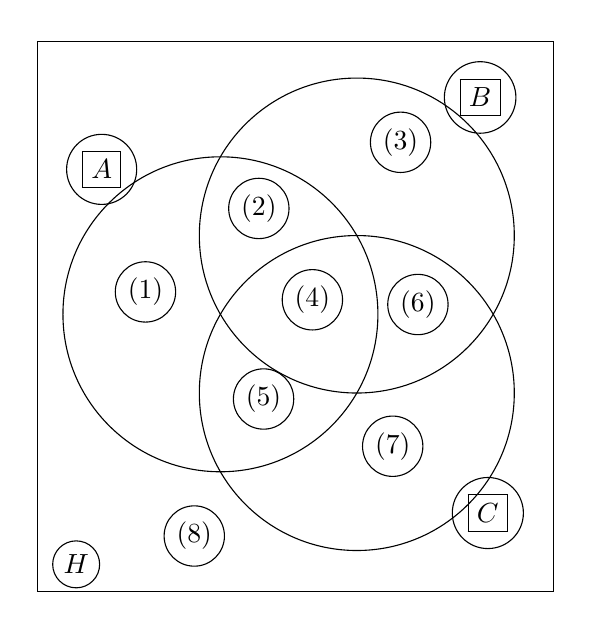
\begin{tikzpicture}[x=1.0cm,y=1.0cm]
\clip(-4.18,-0.72) rectangle (2.64,6.64);
\draw(-1.7320508075688772,3.) circle (2.cm);
\draw(0.,4.) circle (2.cm);
\draw(0.,2.) circle (2.cm);
\draw (-4.06,6.46)-- (2.5,6.46);
\draw (2.5,6.46)-- (2.5,-0.52);
\draw (2.5,-0.52)-- (-4.06,-0.52);
\draw (-4.06,-0.52)-- (-4.06,6.46);
\draw (-3.78,0.04) node[anchor=north west] {$H$};
\draw (-2.96,3.56) node[anchor=north west] {$(1)$};
\draw (-1.52,4.62) node[anchor=north west] {$(2)$};
\draw (0.28,5.46) node[anchor=north west] {$(3)$};
\draw (-0.84,3.46) node[anchor=north west] {$(4)$};
\draw (-1.46,2.2) node[anchor=north west] {$(5)$};
\draw (0.5,3.4) node[anchor=north west] {$(6)$};
\draw (0.18,1.6) node[anchor=north west] {$(7)$};
\draw (-2.34,0.46) node[anchor=north west] {$(8)$};
\draw (-3.56,5.16) node[anchor=north west] {\fbox{$A$}};
\draw (1.24,6.08) node[anchor=north west] {\fbox{$B$}};
\draw (1.34,0.8) node[anchor=north west] {\fbox{$C$}};
\end{tikzpicture}
\end{center}

\noindent Mely tartományokkal állnak a következő halmazok:
$(A{\cup}B){\cap}C$; $A{\cup}(B{\cap}C)$; $(A{\cap}B){\cup}C)$; $A{\cup}(B{\setminus}C)$;
$(B{\setminus}C){\cup}A$; $(B{\setminus}C){\cap}A$; $B{\setminus}(C{\cap}A)$; $B{\setminus}(C{\cup}A)$?

\item Az előző ábrán jelölt tartományok közül melyekből állnak a következő halmazok:
$\overline{A{\cup}B}$, $\overline{B{\cap}C}$, $\overline{C{\setminus}A}$, $\overline{(A{\setminus}B){\setminus}C}$, $\overline{(A{\cup}B){\cap}C}$, $\overline{A{\cap}(B{\cup}C)}$?

\item Ha $A{\setminus}B{=}{\varnothing}$, akkor mivel egyenlő 
$A{\cup}B$, $A{\cap}B$, $B{\setminus}A$?
\end{enumerate}


\subsection*{2008.11.25.}
\underline{Definíció:} $A{\subseteq}B$ ($A$ részhalmaza $B$-nek),
ha $x{\in}A \Rightarrow x{\in}B$.
\begin{enumerate}
\item Igazoljuk a következőket:
\begin{abc2}
\item $A{\subseteq}B$ és $B{\subseteq}A \Rightarrow A{=}B$;
\item $A{\subseteq}B$ és $B{\subseteq}C \Rightarrow A{\subseteq}C$.
\end{abc2}

\item Igazoljuk, hogy ha $A{\subseteq}B$, akkor $A{\cup}B=B$ és $A{\cap}B{=}A$,

\item Legyenek $A$ és $B$ véges halmazok ($|A|$ jelöli $A$ elemeinek számát). Igazoljuk:
\begin{abc2}
\item $|A{\cup}B|\le|A|+|B|$;
\item $|A{\cap}B|\le{\frac{|A|+|B|}{2}}$.
\end{abc2}

\item Adjunk példát olyan $A$, $B$ és $C$ halmazra, hogy teljesüljenek a következő feltételek:\\
$|A|{=}|B|{=}|C|{=}2$, $|A{\cap}B{\cap}C{=}1$ és $A{\not=}B$, $B{\not=}C$.

\item Adjunk meg három olyan kételemű halmazt, melyeknek páronként vett közös része nem üres, de a három halmaz része üres.

\item Az $A$ és $B$ halmazokról tudjuk, hogy 
$A{\cup}B{=}\{1,2,3,4,5,6\}$, $A{\setminus}B{=}\{2,4,6\}$, $A{\cap}B{=}\{1,3\}$.\\
Mik lehetnek $A$ elemei és $B$ elemei?
\end{enumerate}


\subsection*{2008.11.27.}
\begin{enumerate}

\item Definíció: $A{\bigtriangleup}B{=}(A{\setminus}B){\cup}(B{\setminus}A)$;
igazoljuk, hogy
\begin{abc2}
\item $A{\bigtriangleup}B{=}B{\bigtriangleup}A$;
\item $|A{\bigtriangleup}B|{=}|A|+|B|-2|A{\cap}B|$.
\end{abc2}

\item Igazoljuk a következő azonosságokat:
\begin{abc2}
\item $(A{\bigtriangleup}B){\bigtriangleup}C{=}A{\bigtriangleup}(B{\bigtriangleup}C)$;
\item $A{\bigtriangleup}(A{\bigtriangleup}B){=}B$;
\item $(A{\bigtriangleup}B){\cap}C{=}(A{\cap}C){\bigtriangleup}(B{\cap}C)$.
\end{abc2}

\item Az $A$, $B$, $C$ halmazokról tudjuk, hogy $A{\setminus}B{=}\{4,6,8\}$, $B{\setminus}C{=}\{2,5,9,10\}$, $C{\setminus}A{=}\{3,7,11\}$, $A{\cap}B{\cap}C{=}
\{1\}$, $A{\cup}B{=}\{1,2,3,4,5,6,8,9,10,11\}$, $C{\cup}A{=}\{1,2,3,4,5,6,7,8,9,11\}$, és $|C|{=}5$.
\\Határozzuk meg az $A$, $B$, $C$ halmazokat.

\item Az $A$ és $B$ halmazokról tudjuk, hogy $|A|{=}5$, $|B|{=}8$, $|A{\setminus}B|{=}3$.
Számítsuk ki $|A{\cup}B|$ és $|A{\cap}B|$ értékét.

\item Ha $A{=}\{100$-nál nem nagyobb pozitív négyzetszámok$\}$,
 $B{=}\{$a $9$-cel osztható legfeljebb kétjegyű pozitív egészek$\}$,
 akkor számítsuk ki $|A|$, $|B|$,  $|A{\setminus}B|$, $|B{\setminus}A|$,
 $|A{\cup}B|$, $|A{\cap}B|$ értékét.
\end{enumerate}

\subsection*{2008.12.01.}
\begin{enumerate}
\item Tudjuk, hogy $|A|{=}8$, $|B|{=}11$. Mekkora 
lehet $|A{\cap}B|$, $|A{\cup}B|$, $|A|{\setminus}|B|$,
$|A{\cap}B|$ ?

\item Tudjuk, hogy $|A{\cup}B|{=}6$, $|A{\setminus}B|{=}3$,
$|A{\cap}B|{=}2$. Mekkora lehet $|A|$ és $|B|$ ?

\item Az $A$, $B$, $C$ halmazokról tudjuk, hogy $|A{\setminus}B|{=}5$, $|B{\setminus}C|{=}5$, $|C{\setminus}A|{=}4$, 
$|A{\cap}B{\cap}C|{=}1$, $|A{\cup}B|{=}13$, $|A{\cup}C|{=}12$, $|C|=7$.
 Mennyi lehet $|A|$ és $|B|$?

\item Tudjuk, hogy $|A{\cup}B|{=}7$, $|A{\cup}C|{=}7$, $|B{\cup}C|{=}6$.
 Mennyi az a legkisebb és legnagyobb érték, amit $|A{\cup}B{\cup}C|$ felvehet?

\item Tudjuk, hogy $|A|{=}7$, $|B|{=}8$, $|C|{=}9$, $(A{\cap}B{\cap}C){=}3$.
 Mennyi az a legkisebb és legnagyobb érték, amit $|A{\cup}B{\cup}C|$ felvehet?

\item Adjunk meg 4 olyan halmazt, amelyekre teljesül az alábbi feltételek mindegyike:
\\(1) bármely kettőnek van közös eleme;
\\(2) bármely három halmaz metszete üres halmaz;
\\(3) a halmazok elemszáma egyenlő;
\\(4) a halmazok elemszáma a lehető legkisebb.
\end{enumerate}

\subsection*{2008.12.02}
\underline{Definíció}: $A{\times}B{=}\{(a;b)|$ $a{\in}A$, $b{\in}B\}$ \\
Például: $A{=}\{1,2\}$, $B{=}\{3,4\}$ $\Rightarrow$ $A{\times}B{=}\{(1;3),(1;4),(2;3),(2;4)$.

\begin{enumerate}
\item Legyen $A{=}B{=}\{0,1,2\}$ adjuk meg az $A{\times}B$ halmazt.

\item $A{=}\{1,2,3\}$, $B{=}\{2,3,4\}$. Hány eleme van a következő halmazoknak $(A{\setminus}B){\times}(B{\setminus}A)$; $(A{\cup}B){\times}(B{\cap}A)$?

\item Legyen $A$ a $100$-nál nem nagyobb pozitív halmazok száma, B pedig a $200$-nál nem nagyobb pozitív számok halmaza. Mennyi eleme van  az $(A{\times}B){\setminus}(B{\times}A)$ és a $(B{\times}A){\setminus}(A{\times}B)$ halmaznak?

\item $A$ és $B$ olyan véges halmazok, amelyre teljesül, hogy $|A{\times}B|{=}100$. Határozzuk meg $|A{\cup}B|$ és $|A{\cap}B|$ minimumát és maximumát.

\item Legyen $A$, $B$, $C$ amelyekre $|A|{=}|B|{=}|C|{=}5$ $|A{\cup}B{\cup}C|{=}1$. Határozzuk meg $|A{\cup}B{\cup}C|$ minimális és maximális értékét.

\item  Igazoljuk: $A{\setminus}(B{\cup}C){=}(A{\setminus}B){\cap}(A{\setminus}C)$ és $A{\setminus}(B{\cap}C){=}(A{\setminus}B){\cup}(A{\setminus}C)$
\end{enumerate}

\subsection*{2008.12.03}
\begin{enumerate}
\item Legyen $A{=}\{3$-mal osztható kétjegyű számok\}, $B{=}\{7$-tel osztható kétjegyű számok\}. $|A{\cup}B|{=}$? és $|A{\cap}B|{=}$?

\item $A{=}\{1,2\}$, $B{=}\{1,2,3,4\}$, Írjuk fel az $(A{\times}A){\cap}(B{\times}B)$ halmaz elemeit.

\item $A{=}\{1,2,3,4\}$, $A{\cup}B{=}A$, $A{\cap}B{=}B$ mi lehet a $B$ halmaz?

\item Legyen $H{=}{\frac{2}{1}, \frac{4}{3}, \frac{6}{5}, {\ldots}, \frac{1002}{1001}}$. Hány olyan $x$ eleme van a $H$ halmaznak amelyre, $|x-1|<0,1$?

\item Egy osztály létszáma $30$. Az osztályban $3$ nyelvet tanulnak, angolt, németet és franciát és minden diák legalább egy nyelvet tanul. Angolul $14$-en, németül $15$-en, franciául $5$-en tanulnak. Pontosan két  nyelvet $6$ diák tanul. Hányan tanulják mindhárom nyelvet?

\item $|A|{=}7$, $|B|{=}8$, $|C|{=}9$, $|A{\cap}B{\cap}C|{=}3$,  ?${\le} |A{\cup}B{\cup}C|{\le}$?

\item ($*$) Adjunk meg három olyan halmazt, amelyeknek végtelen sok eleme van, bármely kettő is végtelen halmaz, a három halmaz közös része üres.
\end{enumerate}


\section{Függvények}

\subsection*{2008.12.09. -- Függvények}
\begin{enumerate}
\item Ábrázoljuk a következő függvényeket:
\begin{abc4}
\item $f(x) = 2x-1$;
\item $g(x) = x+3$;
\item $h(x) = -x+2$;
\item $k(x) = -\frac{1}{2}x+2$.
\end{abc4}
\item Ábrázoljuk a következő függvényeket:
\begin{abc4}
\item $x\mapsto |x|$;
\item $x\mapsto |x-2|$;
\item $x\mapsto |x+1|$;
\item $x\mapsto |x+2|+|x-3|$.
\end{abc4}
\item Ábrázoljuk a következő függvényeket:
\begin{abc4}
\item $x\mapsto 2|x|$;
\item $x\mapsto |2x|$;
\item $x\mapsto |x|-2$;
\item $x\mapsto |x-2|-|x-3|$.
\end{abc4}

\end{enumerate}

\subsection*{2008.12.10.}
\begin{enumerate}
\item Ábrázoljuk:
\begin{abc3}
\item $x\mapsto |2x-1|$;
\item $x\mapsto |x-1|-|x+3|$;
\item $x\mapsto |\frac12 x+1|$;
\item $x\mapsto |3x-2|$;
\item $x\mapsto \frac{|x|}{2}$;
\item $x\mapsto |2x-1|+|x+1|$;
\item $x\mapsto \left||x|-2\right|$;
\item $x\mapsto \left||x-2|-1\right|$;
\item $x\mapsto ||||x|-3|-2|-1|$.
\end{abc3}
\end{enumerate}

\subsection*{2008.12.11.}
\begin{enumerate}
\item Ábrázoljuk a derékszögű koordináta-rendszerben azokat a 
$P(x;y)$ pontokat, amelyeknek koordinátáira igaz a következő összefüggés:
\begin{abc3}
\item $x\ge y$;
\item $|x|\ge |y|$;
\item $|x-1|\le 1$;
\item $|x+1|\ge 1$;
\item $|x+1|+|y-1|\le 2$.
\end{abc3}
\item Ábrázoljuk a következő függvényeket:
\begin{abc3}
\item $x\mapsto |||x-1|-2|-3|$;
\item $x\mapsto |x+2|+|x|+|x-3|$;
\item $x\mapsto ||x+3|-|x-2||$;
\item $x\mapsto x-|x|$;
\item $x\mapsto |2|x|-x|$.
\end{abc3}

\end{enumerate}

\subsection*{2008.12.16.}
Ábrázoljuk a következő függvényeket:
\begin{enumerate}
\item $x\mapsto ||x-3|-|x+1||$;
\item $x\mapsto ||x|+|x-2|-|x+1|$;
\item $x\mapsto |x+2|+|x|+|x-3|$;
\item $x\mapsto |x+3|+|x+1|+|x-2|+|x-4|$;
\item $x\mapsto |2x-1|-|2x+1|$;
\item $x\mapsto ||x-3|-|x|-|x+1||$;
\item $x\mapsto |3|x|-|x-1||$;
\item $x\mapsto |2x-3|+|2x-4|$.
\end{enumerate}

\subsection*{2008.12.18.}
\begin{enumerate}
\item Öt gyufásdobozra ráírtuk a bennük található gyufaszálak számát. A gyufásdobozok egy kör kerülete mentén helyezkednek el. Szomszédos dobozokból 
lehet átrakni egymásba gyufaszálakat. A cél az, hogy minden gyufásdobozban azonos számú gyufaszál legyen és az összes átrakott gyufaszálak száma a lehető legkevesebb legyen.
\begin{center}
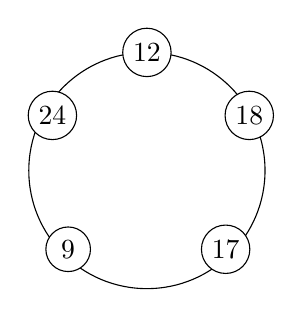
\begin{tikzpicture}[x=1.0cm,y=1.0cm, fill=white]
\draw(2,2) circle (1.5cm);
\draw (2,3.5) node[fill=white,draw] {12};
\draw (3.3,2.7) node[fill=white,draw] {18};
\draw (0.8,2.7) node[fill=white,draw] {24};
\draw (1,1) node[fill=white,draw] {\,9\,};
\draw (3,1) node[fill=white,draw] {17};
\end{tikzpicture}
\end{center}

\newpage
\item Az 1. feladatban megfogalmazott célt kell elérni, ha a gyufásdobozokban
a gyufaszálak száma:
\begin{abc2}
\item ~

\begin{center}
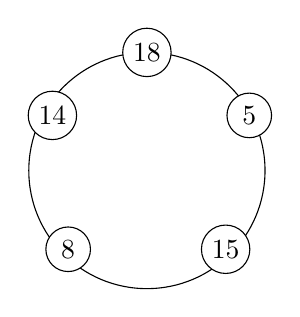
\begin{tikzpicture}[x=1.0cm,y=1.0cm, fill=white]
\draw(2,2) circle (1.5cm);
\draw (2,3.5) node[fill=white,draw] {18};
\draw (3.3,2.7) node[fill=white,draw] {\,5\,};
\draw (0.8,2.7) node[fill=white,draw] {14};
\draw (1,1) node[fill=white,draw] {\,8\,};
\draw (3,1) node[fill=white,draw] {15};
\end{tikzpicture}
\end{center}

\item ~

\begin{center}
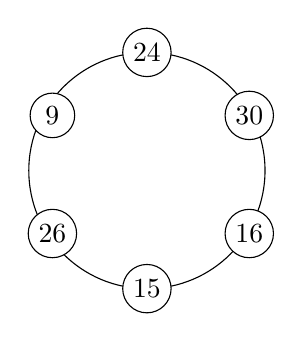
\begin{tikzpicture}[x=1.0cm,y=1.0cm, fill=white]
\draw(2,2) circle (1.5cm);
\draw (2,3.5) node[fill=white,draw] {24};
\draw (3.3,2.7) node[fill=white,draw] {30};
\draw (0.8,2.7) node[fill=white,draw] {\,9\,};
\draw (3.3,1.2) node[fill=white,draw] {16};
\draw (0.8,1.2) node[fill=white,draw] {26};
\draw (2,0.5) node[fill=white,draw] {15};
\end{tikzpicture}
\end{center}

\end{abc2}
\end{enumerate}

\subsection*{2009.01.06. -- Ismétlő feladatok}
Ábrázoljuk a következő függvényeket:
\begin{enumerate}
\item $x\mapsto ||x+2|-|x-1||$;
\item $x\mapsto |x+3|+|x|+|x-4|$;
\item $x\mapsto |2|x|-|x+1||$;
\item $x\mapsto |x-1|+x+|x+1|$;
\item $x\mapsto |2x-|x-1|-|x+1||$.
\end{enumerate}


\subsection*{2009.01.07. -- Függvények}
Ábrázoljuk a következő függvényeket:
\begin{enumerate}
\item $x\mapsto ||x-2|-1|-1$;
\item $x\mapsto |2x-1|-|2x+1|$;
\item $x\mapsto ||x+2|-|x|-|x-2||$;
\item $x\mapsto |x+3|+|x|+|x-2|$;
\item $x\mapsto |2x|-|x|+|x-1|$.
\end{enumerate}


\subsection*{2009.01.12.}
Ábrázoljuk:
\begin{enumerate}
\item $x\mapsto [2x]$;
\item $x\mapsto [x-1]$;
\item $x\mapsto [x]+[-x]$;
\item $x\mapsto [~|x|~]$;
\item $x\mapsto \big|[x]\big|$;
\item $x\mapsto x\cdot [x]$;
\item $x\mapsto \dfrac{x}{[x]}$, $x<0$ vagy $x\ge 1$.
\end{enumerate}


\subsection*{2009.01.14.}
\begin{enumerate}
\item Ábrázoljuk:
\begin{abc2}
\item $x\mapsto \dfrac{x}{[x]}$, $x<0$ vagy $x\ge 1$;
\item $x\mapsto x-[x]$;
\item $x\mapsto [2x]-[x]$;
\item $x\mapsto [x]\cdot[-x]$;
\item $x\mapsto [2x]-2[x]$.
\end{abc2}
\item Hol vannak a síkon azok a $P(x;y)$ pontok, amelyeknek koordinátáira teljesül:
\begin{abc3}
\item $x=[y]$;
\item $[x]=y$;
\item $[x]=[y]$?
\end{abc3}
\end{enumerate}


\subsection*{2009.01.15.}
\begin{enumerate}
\item Ábrázoljuk a következő függvényeket:
\begin{abc3}
\item $x\mapsto x\cdot \left[\dfrac{1}{x}\right]$, ha $x\ne 0$;
\item $x\mapsto [x]+\left[x+\frac{1}{2}\right]$;
\item $x\mapsto [x]+\left[x+\frac{1}{3}\right]+\left[x+\frac{2}{3}\right]$.
\end{abc3}
\item Oldjuk meg a következő egyenleteket:
\begin{abc2}
\item $[x]+\left[x+\frac{1}{2}\right]=[2x]$;
\item $\left[\dfrac{[x]}{2}\right]=\left[\dfrac{x}{2}\right]$.
\end{abc2}
\item Hol vannak a síkon azok a $P(x;y)$ pontok, amelyeknek
koordinátái kielégítik a következő feltételt:
\begin{abc2}
\item $[x]+[y]=1$;
\item $[x]\cdot [y]=4$?
\end{abc2}

\end{enumerate}


\subsection*{2009.01.26.}
\begin{enumerate}
\item Ábrázoljuk a következő függvényeket:
\begin{abc4}
\item $x\mapsto \big|[x]\big|+[~|x|~]$;
\item $x\mapsto [x]\cdot x+\sgn x$;
\item $x\mapsto [x]+[2x]$;
\item $x\mapsto [x+2]+[x]$.
\end{abc4}

\item Hol vannak a síkon azok a pontok, amelyeknek a koordinátáira teljesül:

\begin{abc3}  
\item $2[x]=[y]$;
\item $[x][y]=8$;
\item $[x]+[y]=-2$.
\end{abc3}

\end{enumerate}

\subsection*{2009.01.27.}
\begin{enumerate}
\item Egy kétjegyű szám számjegyeinek összege 12. Ha számjegyeit felcseréljük, 18-cal nagyobb számot kapunk. Melyik ez a szám?
\item Egy könyv ára vászonkötésben 1680~Ft, ami 68\%-kal több, mint papírkötésben. Mennyi az ára a papírkötésű könyvnek?
\item Egy téglalap egyik oldalát 25\%-kal megnöveltük. Hány \%-kal kell a másik oldalát csökkenteni, hogy a területe ne változzon?
\item 850-et osszuk szét két részre úgy, hogy az első rész 8\%-ának és a második rész 24\%-ának az összege 850-nek a 12\%-a legyen.
\item Egy kertet az apa 3,5 óra alatt, a fia 6 óra alatt ásná fel egyedül. 
Mennyi idő alatt készülnek el a kert a felásásával, ha mindketten dolgoznak?
\item Több testvér osztozik az örökségen. $A$ kap 20 ezer~Ft-ot és a maradék tizedrészét, $B$ kap 40 ezer~Ft-ot és a maradék tizedrészét, és így tovább.
Végül kiderült, hogy minden testvér ugyanannyit kapott. Hányan voltak, mennyi volt az örökség és mennyit kaptak külön-külön?
\end{enumerate}


\subsection*{2009.02.03.}
\begin{enumerate}
\item Oldjuk meg a következő egyenleteket:

\begin{abc4}
\item $|x-2|=3$;
\item $|x-4|=5$;
\item $|2x-1|=3$;
\item $|2x-5|=x-1$.
\end{abc4}

\item Oldjuk meg függvénygrafikonok felhasználásával:

\begin{abc3}
\item $x+|x|=4$;
\item $|x|=2x+1$;
\item $|x-3|=x$.
\end{abc3}

\item Oldjuk meg a következő egyenleteket: 

\begin{abc3}
\item $||x|-1|=4x+4$;
\item $||x|-2|=1$;
\item $||x+2|-3|=1$.
\end{abc3}

\end{enumerate}


\subsection*{2009.02.09.}
\begin{enumerate}
\item Ha egy kétjegyű szám kétszereséből 1-et kivonunk, akkor egy olyan kétjegyű számot kapunk, amely az eredeti szám számjegyeinek felcserélésével keletkezik. Melyik ez a szám?
\item 76870~Ft illetéket kell megfizetni illetékbélyeggel. 10, 50 és 100~Ft-os
bélyegeket veszünk, 50~Ft-osból éppen kétszer annyit, mint a másik kettőből együtt. Milyen esetek lehetségesek?
\item Oldjuk meg:
\begin{abc3}
\item $|x+2|>|x|$;
\item $|x-1|<|x|$;
\item $||2x-1|-3|>2$;
\item $|2x-3|>|3x+7|$;
\item $|x+1|+|x-4|>4$;
\item $\dfrac{1}{|x|-3}<\dfrac{1}{2}$.
\end{abc3}
\end{enumerate}


\subsection*{2009.02.10.}
\begin{enumerate}
\item A 100-at bontsuk fel két részre úgy, hogy az egyik rész 5-tel osztva 2-t, a másik rész 7-tel osztva 4-et adjon maradékul.
\item Melyik az a kétjegyű szám, amely számjegyeinek 2-szeres szorzatával egyenlő?
\item ($*$) Melyik az négyjegyű szám, amely 132-vel osztva 105-öt, 133-mal 
osztva 91-et ad maradékul?
\item Oldjuk meg:
\begin{abc4}
\item $\dfrac{2x-3}{3x-6}>0$;
\item $\dfrac{x-4}{2x-3}\le 0$;
\item $\dfrac{5-x}{x-4}\le 0$;
\item ($*$) $\dfrac{3x}{2x+1}>1$;
\item $\dfrac{5x-5}{3x-2}>1$.
\end{abc4}
\end{enumerate}


\subsection*{2009.02.11.}
\begin{enumerate}
\item Egy kétjegyű számban az egyesek száma 3-mal több, mint a tízesek száma.
Ha a szám két számjegye közé harmadik számjegyként a két számjegy összegét iktatjuk be, akkor az így kapott háromjegyű szám az eredeti szám 11-szerese.
Melyik lehet ez a kétjegyű szám?
\item Három golyógyűjtő gyerek $A$, $B$ és $C$ játszik. 
Egy játéknak mindig egy vesztese van. Megállapodnak abban, hogy a mindenkori 
vesztes a másik két játékos golyókészletét megháromszorozza. Három játék után,
amelyeket sorra $A$, $B$ és $C$ veszített el, mindegyik játékosnak ugyanannyi golyója lett. Tudjuk még, hogy az első játszma után $C$-nek 54 golyóval volt 
többje, mint $A$-nak. Hány golyója volt eredetileg $A$-nak, $B$-nek és $C$-nek?
\item Oldjuk meg:
\begin{abc2}
\item $\dfrac{x+2}{(x-3)^2}>0$;
\item $\dfrac{2x+1}{3x+2}<0$;
\item $|x-1|+|2-x|>3+x$;
\item ($*$) $[x-1]=\left[\dfrac{x+2}{2}\right]$.
\end{abc2}
\end{enumerate}


\subsection*{2009.02.16.}
\begin{enumerate}
\item Egy apa háromszor annyi idős, mint a fia.
7 évvel ezelőtt 5-ször annyi idős volt. Hány év múlva
lesz kétszer annyi idős, mint a fia?
\item András és Béla együtt 70 évesek. András kétszer annyi idős, mint Bála volt akkor, amikor András annyi idős volt, mint Béla most. Hány éves Béla?
\item Egy medencébe 3 csövön keresztül folyhat be a víz. Az első cső 4, a második 6, a harmadik 12 óra alatt tölti tele egyedül a medencét. Mennyi 
idő alatt telik meg a medence, ha mindhárom cső egyszerre nyitva van?
\item Oldjuk meg:
\begin{abc4}
\item $\dfrac{7-2x}{4+3x}>0$;
\item $\dfrac{2x+3}{x-2}<1$;
\item $\dfrac{3x}{x-3}\ge 2$;
\item $\dfrac{5x-2}{x-1}+\dfrac{2}{3}\le \dfrac{3x+4}{x-1}$.
\end{abc4}
\end{enumerate}


\subsection*{2009.02.17.}
\begin{enumerate}
\item Volt egyszer két testvér, kettejüknek volt egy birkanyája. Egyszer csak eladták a birkákat, s minden birkáért pontosan annyit kaptak, ahány birkájuk volt összesen. A kapott pénzt a következőképpen osztották el: először az
idősebb testvér vett el magának 10 rubelt, majd az öccse 10 rubelt, aztán
megint az idősebb fiú vett el 10 rubelt, és így tovább. Utoljára a fiatalabbnak már nem jutott 10 rubel, ezért elvette az aprópénzt, s hogy igazságos legyen az osztozkodás, az idősebbik nekiadta a bicskáját. Mennyit ért a bicska?
\item A felírt bűvös négyzetben minden sorban és minden oszlopban, továbbá mindkét átlóban ugyanannyi a számok összege. Határozzuk meg a hiányzó számokat!

\centerline{
\begin{tabular}{|c|c|c|}
\hline
199&995&~~~\cr
\hline
~~~&~~~&~~~\cr
\hline
~~~&~~~&1995\cr
\hline
\end{tabular}}
\end{enumerate}


\subsection*{2009.02.18.}
\begin{enumerate}
\item Oldjuk meg:
\begin{abc2}
\item $\dfrac{1}{1+\dfrac{1}{1+\dfrac{1}{1+\dfrac{1}{x}}}}=\dfrac{3}{5}$;\smallskip
\item $\dfrac{x-1}{2009}+\dfrac{x-2}{2008}+\dfrac{x-3}{2007}=3$;\smallskip
\item $\dfrac{3x+5}{7}+\dfrac{10-3x}{5}<\dfrac{2x+7}{3}$;
\item $(x+3)^2-(x+1)^2<4$;
\item $5-(x-2)^2>(9-x^2)+7$;
\item $\left.
\begin{aligned}
3x+1&>x+12~\text{és}\\
4x-6&<3x+18
\end{aligned}
\right\}$;
\item $\dfrac{3x-1}{2}-\dfrac{5-2x}{3}>2x+1$.
\end{abc2}

\end{enumerate}


\subsection*{2009.02.19.}
\begin{enumerate}
\item Oldjuk meg:
\begin{abc4}
\item $\left|\dfrac{3x-2}{x-1}\right|=2$;
\item $\left|\dfrac{3|x|-2}{|x|-1}\right|=2$;
\item $\dfrac{2-3|x|}{1+|x|}=1$;
\item $\left|\dfrac{2-3|x|}{1+|x|}\right|=1$.
\end{abc4}
\item Oldjuk meg:
\begin{abc3}
\item $\dfrac{2}{|x-4|}>1$;
\item $\dfrac{2}{|x+2|}\le 1$;
\item $\dfrac{2}{|x-13|}>\dfrac{8}{9}$.
\end{abc3}
\item Ábrázoljuk a derékszögű koordináta-rendszerben azokat
a $P(x;y)$ pontokat, amelyekre
$$||x|-|y||<1.$$
\end{enumerate}


\subsection*{2009.02.24. -- Ismétlő feladatok}
\begin{enumerate}
\item 

\begin{abc3}
\item $\dfrac{x}{2}-\dfrac{2x}{3}+\dfrac{5x}{6}-3=\dfrac{x}{4}+1$;
\item $\dfrac{3}{x(2x-1)}+\dfrac{5}{x}=\dfrac{1}{2x-1}$;
\item $\dfrac{12x-9}{3x-2}+\dfrac{6x-5}{2-3x}=2$.
\end{abc3}
\item 
\begin{abc4}
\item $\dfrac{2}{x-4}\ge \dfrac{5}{x-4}-3$;
\item $\dfrac{3-5x}{2+x}>-4$;
\item $\dfrac{2x+3}{x-2}<1$;
\item $1-\dfrac{3x-2}{2x+5}\ge 3$.
\end{abc4}

\end{enumerate}


\section{Valószínűségszámítás}

\subsection*{2009. 03. 05.}
\begin{enumerate}
\item Egy kockával 5-ször dobunk. Mennyi a valószínűsége, hogy az 5 dobásból 0, 1, 2, 3, 4, 5, 6-ost dobunk? Készíts táblázatot!

\item Egy pénzérmével 6-szor dobunk. Mennyi a valószínűsége, hogy 0, 1, 2, 3, 4, 5, 6 fejet dobunk? Készíts táblázatot!

\item Dobjunk fel egy érmét. Ha az eredmény fej, még egyszer dobunk, ha írás, még kétszer. Mennyi a valószínűsége, hogy összesen egy fejet dobunk?

\item 100 alma közül 10 kukacos. Véletlenszerűen kiveszünk az almák közül 5-öt. Mennyi a valószínűsége, hogy lesz a kiválasztott almák között kukacos?

\item Tíz kockával dobunk, mennyi annak a valószínűsége, hogy a dobott számok összege legalább 58?

\item Egy pénzdarabot 10-szer feldobunk és az eredményeket leírjuk, ha fej jön ki F-et, ha írás I-t írunk. Mennyi a valószínűsége, hogy az így kapott 10 elemű szorzat tartalmaz két azonos betűt egymás mellett?
\end{enumerate}
\subsection*{2009. 03. 10.}
\begin{enumerate}
\item Öt levelet megírt valaki 5 ismerősének, majd borítékokba rakta a leveleket. Ezután a lezárt borítékokat véletlenszerűen megcímzi. Mennyi a valószínűsége, hogy legalább 3 ismerőse a neki szánt levelet kapja meg? Mennyi a valószínűsége, hogy senki sem kapja meg a neki szánt levelet? 

\item Az 1, 2, 3, 4, 5 számjegyeket véletlenszerűen egymás mellé írjuk. Mennyi a valószínűsége, hogy a kapott ötjegyű szám osztható 8-cal?

\item Három kockával dobunk. Mennyi a valószínűsége, hogy a dobott számok négyzetösszege osztható 3-mal?

\item Mennyi a valószínűsége, hogy a lottón kihúzott öt számban mind a 10 számjegy előfordul (az egyjegyű számokat tekintsük olyan kétjegyűnek, amelynek az első jegye 0)?

\item Mennyi a valószínűsége, hogy véletlenül kiválasztott 12 ember születésnapja különböző hónapban legyen?

\item Jelölje $A_k$ annak a valószínűségét, hogy kockát $k$-szor feldobva először a $k$-adik dobásra kapunk 6-ost. Számoljuk ki $A_1, A_2, A_3, A_4, A_5$ és $A_6$ értékét!
\end{enumerate}
\subsection*{2009. 03. 17.}
\begin{enumerate}
\item A kockadobás várható értékét így számítjuk ki: 

$$
\begin{array}{c}
\text{ki: dobott szám}\cr
X:\text{valószínűség}
\end{array}
\left(
\begin{array}{cccccc}
1&2&3&4&54&6\cr
\frac{1}{6}&
\frac{1}{6}&
\frac{1}{6}&
\frac{1}{6}&
\frac{1}{6}&
\frac{1}{6}
\end{array}
\right)
$$

$$
E(X)=
1\cdot\frac{1}{6}+
2\cdot\frac{1}{6}+
3\cdot\frac{1}{6}+
4\cdot\frac{1}{6}+
5\cdot\frac{1}{6}+
6\cdot\frac{1}{6}=
\frac{21}{6}=3{,}5
$$








\item Számítsuk ki a két kockával dobott pontok összegének várható értékét.

\item Egy érmével dobunk. Ha az eredmény fej, még kétszer dobunk, ha írás, még egyszer. Mennyi az összes fej dobások várható értéke?

\item Péter feldob egy kockát. Ha páratlan számot dob, veszít 10 Ft-ot, ha 6-ost dob, nyer 40 Ft-ot, ha 2-est vagy 4-est dob, újra dobhat. A második dobásnál 10 Ft-ot nyer, ha párosat dob és 20 Ft-ot veszít, ha páratlant dob. Döntsük el, hogy a játék Péter számára előnyös, hátrányos vagy igazságos.

\item Egy érmével addig dobunk, amíg először fordul elő, hogy két egymás utáni dobás azonos. Mennyi a szükséges dobások várható száma?
\end{enumerate}
\subsection*{2009. 03. 18.}
\begin{enumerate}
\item Két kockával dobunk. Számítsuk ki a dobott számok 
\begin{abc}
\item maximumának
\item minimumának
\end{abc}
\quad várható értékét!

\item Mennyi a lottótalálatok számának várható értéke egy találomra kitöltött szelvény esetén? (ötös lottón)

\item Egy urnában van 5 piros, 3 fehér és 2 kék golyó. Háromszor húzunk:
\begin{abc2}
\item visszatevés nélkül
\item visszatevéssel.
\end{abc2}
Határozzuk meg mindkét esetben a kihúzott piros golyók várható számát!

\item Egy urnában 100 cédula van 1-től 100-ig számozva. Kihúzunk ezek közül 15 darabot visszatevéssel. Mennyi a kihúzott számok összegének várható értéke?

\item Mennyi az ötös lottón kihúzott számok összegének várható értéke?
\end{enumerate}
\subsection*{2009. 03. 19.}
\begin{enumerate}
\item Mennyi annak a valószínűsége, hogy egy tetszőlegesen választott pozitív egész szám négyzete 1-re végződik?

\item Mennyi annak a valószínűsége, hogy egy tetszőlegesen választott pozitív egész szám köbe 11-re végződik? 

\item Mennyi annak a valószínűsége, hogy $\binom{m}{3}$ osztható 3-mal, ha $n > 3$, egész szám?

\item Mennyi annak a valószínűsége, hogy egy 12 tagú társaságban mindenkinek más hónapban legyen a születésnapja?

\item Egy vonat 3 kocsijába 9 utas száll be. Minden utas véletlenszerűen választja meg, hogy melyik kocsiba száll. Mennyi annak a valószínűsége, hogy mindhárom kocsiba 3 ember száll? 
\end{enumerate}
\subsection*{2009. 03. 24.}
\begin{enumerate}
\item Az 52 lapos francia kártyából az egyik játékos 12 lapot kap. Mennyi a valószínűsége, hogy legfeljebb 3 ásza lesz?

\item Mennyi annak a valószínűsége, hogy egy 4 tagú társaságban van két ember, akinek az év azonos napján van a születésnapja?

\item Egy urnában van 5 piros és 10 fehér golyó.Visszatevés nélkül addig húzunk, amíg fehéret nem húzunk. Mennyi az eddig kihúzott piros golyók várható száma?

\item Egy társasjátéknál egy korong kerületén 0-tól 25-ig sorban számozott 26 mező van. Minden játékos a 0-val számozott mezőre állítja a bábuját és minden alkalommal, amikor sorra kerül, annyi mezővel lép előre, amennyit egy kockával dob. Ha a bábu a 13 számú mezőre ér, vissza kell mennie a 0-ra. Mennyi a valószínűsége, hogy egy játékos 5 dobásból a 25 számú mezőre ér?
\end{enumerate}
\subsection*{2009. 03. 25.}
\begin{enumerate}
\item Ötször dobunk egy kockával. Mennyi a valószínűsége, hogy a dobott számok összege 25-nél nagyobb szám lesz?

\item Egy urnában 4 piros és 6 fehér golyó van. Kihúzunk 3 golyót
\begin{abc}
\item visszatevéssel;
\item visszatevés nélkül.
\end{abc}
Számítsuk ki mindkét esetben a kihúzott piros golyók várható számát!

\item Egy urnában 4 piros, 4 fehér és 2 zöld golyó van. Az egyik játékos ebből addig húz ki visszatevés nélkül golyókat, amíg az első zöldet húzza. Ekkor a társától, a másik játékostól annyiszor 10 Ft-ot kap, ahány golyót kihúzott. Ezután a maradék golyók közül a másik játékos húzhat addig, amíg zöldet nem húz és ő is annyiszor 10 Ft-ot kap az elsőtől, ahány golyót kihúzott. Igazságos-e a játék?

\item Egy szabályos érmével addig dobunk, amíg először fordul elő, hogy két egymást követő dobás azonos. Mennyi a szükséges dobások várható száma?
\end{enumerate}
\subsection*{2009. 03. 26.}
\begin{enumerate}
\item Péter feldob egy kockát. Ha páratlan számot dob, veszít 10 Ft-ot, ha 6-ost dob nyer 40 Ft-ot, ha 2-est vagy 4-est, újra dobhat. A második dobásnál 10 Ft-ot nyer, ha párost dob és 20 Ft-ot veszít, ha páratlant dob. Döntsük el, hogy a játék Péter számára előnyös, igazságos vagy hátrányos.

\item Három különböző színű kockával dobunk. Mennyi a valószínűsége, hogy a dobott számok összege prímszám?

\item Egy kockával addig dobunk, amíg valamelyik, már korábban dobott szám újra előfordul. Mennyi a szükséges dobások várható száma?

\item Egy urnában van 4 piros és 6 fehér golyó. 5-ször kihúzunk egy golyót úgy, hogy feljegyezzük a számát, visszatesszük, összekeverjük és úgy húzunk újra. Mennyi a kihúzott piros golyók várható száma?
\end{enumerate}
\subsection*{2009. 04. 01.}
\begin{enumerate}
\item ($*$) 15 golyót véletlenszerűen helyezünk el 4 dobozba. Mennyi a valószínűsége, hogy mindegyik dobozba legalább 3 golyó kerül? 

\item Egy dobozban 8 piros és 10 fehér golyó van. Visszatevés nélkül  egymás után húzunk golyókat. Mennyi a valószínűsége, hogy először az 5. húzáskor kerül elő fehér golyó?

\item Egy dobozban 6 piros, 4 kék, 2 zöld golyó van. Visszatevéssel húzunk. 10 Ft-ért fogadhatunk a golyó színekre. Többlet esetén a piros golyónál 20, a kék golyónál 30, zöld golyónál 60 Ft a nyeremény. Melyik golyóra érdemes fogadni? 

\item Állítsuk növekvő sorrendbe a következő események valószínűségét:
\begin{abc}
\item Egy kockával 6-szor dobunk és és legalább 1 db 6-ost dobunk;
\item Egy kockával 12-szer dobunk és legalább 2 db 6-ost dobunk;
\item Egy kockával 18-szor dobunk és legalább 3 db 6-ost dobunk.
\end{abc}
\end{enumerate}
\subsection*{2009. 04. 06.}
\bf{Ismétlő feladatok} \rm
\begin{enumerate}
\item Egy urnában van 4 piros, 4 fehér és 4 zöld golyó. 4-szer húzunk visszatevéssel. Mennyi a kihúzott fehér golyók várható száma?

\item Elemezzük a ,,CRAPS'' játékot. Ebben két kockával dobunk, a dobott pontok összege számít. 
Ha az első dobás eredménye 7 vagy 11, a játékos nyer, ha 2, 3 vagy 12, akkor veszít. Minden más esetben az első dobás eredménye a ,,POINT'' és újra dobhat. 
A második dobástól kezdve a játékos nyer,  ha a ,,POINT''-ot dobja, veszít, ha 7-est dob minden más esetben újra dobhat. Mennyi a játékban a játékos nyerési esélye?
\end{enumerate}



\section{Összegzések}

\subsection*{2009. 04. 15.}
\begin{enumerate}
\item Végezzük el a következő szorzatokat:

\begin{abc4} 
\item $(x-2)\cdot(x+2)$;
\item $(a+b)\cdot(a-b)$;
\item $(2a+3b)\cdot(2a-b)$;
\item $(2xy-1)\cdot(2xy+1)$.
\end{abc4}

\item Végezzük el a következő műveleteket:

\begin{abc}
\item $(x-2)\cdot(x+3)+(x+2)\cdot(x-3)$;
\item $(a-3)\cdot(a+4)+(a+3)\cdot(a-4)$;
\item $(x^2+x+1)\cdot(x^2-x+1)\cdot(x^2-1)$.
\end{abc}


\item A természetes számok sorozatában két egymást követő egész szám négyzetének különbsége 33. Melyik ez a két szám?

\item A természetes számok sorozatában két egymást követő páros szám négyzetének különbsége 28. Melyik ez a két szám?

\item Két szomszédos páratlan szám négyzetének különbsége 64. Melyik ez a két szám?
\end{enumerate}
\subsection*{2009. 04. 16.}
\begin{enumerate}
\item Oldjuk meg a pozitív egész számok körében: 
\quad $\dfrac{1}{x} + \dfrac{1}{y} = \dfrac{1}{14}$.

\item Számítsuk ki a következő összegeket:
\begin{abc}
\item $\dfrac{1}{1\cdot2} + \dfrac{1}{2\cdot3} + \dfrac{1}{3\cdot4} + \cdots + \dfrac{1}{99\cdot100}$;
\item $1\cdot2+2\cdot3+3\cdot4+\cdots+10\cdot101$;
\item $\dfrac{1}{1\cdot2\cdot3}+\dfrac{1}{2\cdot3\cdot4}+\dfrac{1}{3\cdot4\cdot5}+\cdots+\dfrac{1}{98\cdot99\cdot100}$.
\end{abc}

\item Alakítsuk szorzattá:

\begin{abc3}
\item $a^2-4$; 
\item $25-x^2$;
\item $a^2-9b^2$;

\item $4x^2-\dfrac{1}{25}y^2$;
\item $16a^4-9b^2$;
\item $36ta^4-49b^6$.
\end{abc3}

\item Alakítsuk szorzattá:

\begin{abc3}
\item $4(a-b)^2-(a+b)^2$;
\item $(x-2y)^2-4(x+y)^2$;
\item $16(x-y)^2-25(x+y)^2$.
\end{abc3}
\end{enumerate}
\subsection*{2009. 04. 20.}
\begin{enumerate}
\item Számítsuk ki minél egyszerűbben a következő összeget:
$\dbinom{2}{2}+\dbinom{3}{2}+\dbinom{4}{2}+\dbinom{5}{2}\cdots+\dbinom{100}{2}=$ ?

\item Az előző feladat eredményének felhasználásával számítsuk ki: 
$1\cdot2+2\cdot3+3\cdot4+4\cdot5+\cdots+99\cdot100$. 

\item Számítsuk ki: 
$1\cdot2\cdot3+2\cdot3\cdot4+3\cdot4\cdot5+\cdots+98\cdot99\cdot100$.

\item Egy gépkocsi A-ból B-be az utat óránkénti 60 km/ó sebességgel teszi meg. Visszafelé, B-ből A-ba lassabban megy, itt átlagsebessége 50 km/ó. Számítsuk ki a teljes, oda-vissza útra az átlagsebességét. 

\item Egy motorversenyen három motorkerékpáros indul. A második óránként 15 km-rel kevesebbet tesz meg az elsőnél és 3 km-rel többet a harmadiknál. Így a második 12 perccel később ér célba, mint az első, de 3 perccel korábban, mint a harmadik. Számítsuk ki a versenypálya hosszát, az egyes versenyzők sebességét és idejét. 
\end{enumerate}
\subsection*{2009. 04. 21.}
\begin{enumerate}
\item Számítsuk ki a következő összegeket: 
\begin{abc}
\item $\dfrac{1}{1\cdot4}+\dfrac{1}{4\cdot7}+\dfrac{1}{7\cdot10}+\cdots+\dfrac{1}{97\cdot100}$;
\item $1\cdot2\cdot3\cdot4+2\cdot3\cdot4\cdot5+3\cdot4\cdot5\cdot6+\cdots+100\cdot101\cdot102\cdot103$.
\end{abc}
\item Erre az összegre is egyszerű, gyors módszert keress: 
\quad $1+3+5+7+9+\cdots+999$.

\item ($*$) A következő összeget is lehet ötleteket felhasználva egyszerűen kiszámítani:
$1^3+2^3+3^3+4^3+100^3$.

\item ($*$) Itt is kell az egyszerű számoláshoz egy ötlet: 
\begin{abc2}
\item $1+2+2^2+2^3+2^4+\cdots+2^{20}$;
\item $1+3+3^2+3^3+3^4+\cdots+3^{10}$.
\end{abc2}
\end{enumerate}
\subsection*{2009. 04. 22.}
\begin{enumerate}
\item Számítsuk ki a következő összegeket:
\begin{abc}
\item $1\cdot1!+2\cdot2!+3\cdot3!+4\cdot4!+\cdots+20\cdot20!$;
\item $\dfrac{1}{1\cdot3\cdot5}+\dfrac{1}{3\cdot5\cdot7}+\dfrac{1}{5\cdot7\cdot9}+\cdots+\dfrac{1}{101\cdot103\cdot105}$;
\item $1+2\cdot3+3\cdot3^2+4\cdot3^3+5\cdot3^4+\cdots+100\cdot3^{99}$.
\end{abc}

\item Számítsuk ki: $1^3+3^3+5^3+7^3+\cdots+99^3$.

\item Igazoljuk, hogy

\begin{abc2}
\item ($**$) $\dfrac{1}{2}<\dfrac{1}{51}+\dfrac{1}{52}+\cdots+\dfrac{1}{100}<\dfrac{3}{4}$;
\item ($*$) $1+\dfrac{1}{4}+\dfrac{1}{9}+\dfrac{1}{16}+\dfrac{1}{25}+\cdots+\dfrac{1}{10000}<2$.
\end{abc2}
\end{enumerate}
\subsection*{2009. 04. 27.}
\begin{enumerate}
\item Számítsuk ki: 
\begin{abc}
\item $1+\dfrac{1}{2}+\dfrac{1}{4}+\dfrac{1}{8}+\dfrac{1}{16}+\cdots+\dfrac{1}{2^{10}}$;
\item $1+\dfrac{1}{3}+\dfrac{1}{9}+\dfrac{1}{27}+\cdots+\dfrac{1}{3^{20}}$;
\item $1+\dfrac{2}{5}+\dfrac{4}{25}+\dfrac{8}{125}+\cdots+\dfrac{2^{15}}{5^{15}}$.
\end{abc}
\item ($*$) Igazoljuk:
$\dfrac{1}{20}<\dfrac{1\cdot3\cdot5\cdot7\cdot\cdots\cdot99}{2\cdot4\cdot6\cdot\cdots\cdot100}<\dfrac{1}{10}$.
\item Számítsuk ki:
\begin{abc}
\item $\left(1-\dfrac{1}{4}\right)\left(1-\dfrac{1}{9}\right)\left(1-\dfrac{1}{16}\right)\cdots\left(1-\dfrac{1}{169}\right)$;
\item $\left(1-\dfrac{4}{9}\right)\left(1-\dfrac{4}{16}\right)\left(1-\dfrac{1}{25}\right)\cdots\left(1-\dfrac{4}{225}\right)$.
\end{abc}

\item ($*$) $1+\dfrac{1}{2}+\dfrac{1}{3}+\cdots+\dfrac{1}{2^{10}-1}>5$.
\end{enumerate}
\subsection*{2009. 05. 12.}
\begin{enumerate}
\item Számítsuk ki minél egyszerűbben:
\begin{abc}
\item $\dfrac{1}{2}+\dfrac{2}{2^2}+\dfrac{3}{2^3}+\dfrac{4}{3^4}+\dfrac{5}{3^5}+\dfrac{20}{2^{20}}$;
\item $0,9+0,99+0,999+\cdots+0,9999999999$;
\item $\dfrac{1}{225}+\dfrac{2}{225}+\dfrac{3}{225}+\dfrac{4}{225}+\dfrac{5}{225}\cdots+\dfrac{14}{225}$.
\end{abc}

\item Igazoljuk:
\begin{abc}
\item $\dfrac{1}{100}<\dfrac{1}{1000}+\dfrac{4}{1000}+\dfrac{9}{1000}+\cdots+\dfrac{81}{1000}<\left(\dfrac{9}{10}\right)^3$;
\item $\left(1-\dfrac{1}{2^{10}}\right)^{10}<\left(1-\dfrac{1}{2}\right)\left(1-\dfrac{1}{4}\right)\left(1-\dfrac{1}{8}\right)\cdots\left(1-\dfrac{1}{2^{10}}\right)<1-\dfrac{1}{2^{10}}$.
\end{abc}

\item Számítsuk ki:
\begin{abc2}
\item $\dfrac{1+2+2^2+\cdots+2^{20}}{1+3+3^2+\cdots+3^{20}}$;
\item $\dfrac{1}{2}+\dfrac{3}{2^2}+\dfrac{5}{2^3}+\cdots+\dfrac{39}{2^{20}}$.

\end{abc2}
\end{enumerate}
\subsection*{2009. 05. 12.}
\begin{enumerate}
\item Számítsuk ki minél egyszerűbben:
\begin{abc}
\item $1+11+111+\cdots+1111111111=$;
\item $\dfrac{1}{1\cdot4}+\dfrac{1}{4\cdot7}+\dfrac{1}{7\cdot10}+\cdots+\dfrac{1}{97\cdot100}$;
\item $\dfrac{1}{2}+\dfrac{3}{2^2}+\dfrac{5}{2^3}+\cdots+\dfrac{39}{2^{20}}$.
\end{abc}

\item Igazoljuk:
\begin{abc2}
\item ($*$) $\dfrac{1}{19}+\dfrac{1}{20}+\dfrac{1}{21}+\cdots+\dfrac{1}{55}>1$;
\item $\dfrac{1}{2^2}+\dfrac{1}{3^2}+\cdots+\dfrac{1}{10^2}<\dfrac{9}{10}$.
\end{abc2}

\item Igazoljuk, hogy $(10!)^2>10^{10}$.
\end{enumerate}
\subsection*{2009. 05. 13.}
\begin{enumerate}

\item Számítsuk ki minél egyszerűbben:
\begin{abc}
\item $1-\dfrac{1}{2}+\dfrac{1}{4}-\dfrac{1}{8}+\dfrac{1}{16}-\cdots+\dfrac{1}{2^{10}}$;
\item $\dfrac{1}{1\cdot5}+\dfrac{1}{5\cdot9}+\dfrac{1}{9\cdot13}+\cdots+\dfrac{1}{97\cdot101}$;
\item $\left(\dfrac{1}{2}+\dfrac{1}{3}\right)+\left(\dfrac{1}{2^2}+\dfrac{1}{3^2}\right)+\cdots+\left(\dfrac{1}{2^{20}}+\dfrac{1}{3^{20}}\right)$.
\end{abc}
\item Igazoljuk a következő egyenlőtlenségeket:
\begin{abc}
\item $ \dfrac{3}{2}<1+\dfrac{1}{2!}+\dfrac{1}{3!}+\dfrac{1}{4!}+\cdots+\dfrac{1}{10!}<3$;
\item $1+\dfrac{1}{3^2}+\dfrac{1}{5^2}+\dfrac{1}{7^2}+\cdots+\dfrac{1}{19^2}<2$;
\item $\dfrac{15}{2}<1+\dfrac{2}{3}+\dfrac{3}{5}+\dfrac{4}{7}+\cdots+\dfrac{15}{29}$.
\end{abc}

\item Igazoljuk, hogy $10^{11}>11^{10}$.
\end{enumerate}


\section{Gráfok}

\subsection*{2009. 05. 19}
\begin{enumerate}
\item Rajzold meg az összes 4 csúcsú egyszerű gráfot.
\item Van-e olyan egyszerű gráf, amelybn a csúcsőpk fokszáma sorra: \begin{abcn}{3}
\item 1, 3, 3, 4, 4, 2;
\item 1, 3. 4, 4, 2;
\item 2, 3, 3, 4, 4 ?
\end{abcn}
\item Hány 6 csúcsú, legalább 12 élű egyszerű gráf van?
\item Egy 5 csúcsú egyszerű gráfnak 8 éle van. Mekkorák lehetnek a csúcsok fokszámai?
\item Igazoljuk, hogy bármely egyszerű gráfban a  páratlan fokú csúcsok száma páros.
\item Igazoljuk, hogy bármely egyszerű gráfban, ha legalább 2 csúcs van, van 2 azonos fokszámú csúcs.
\end{enumerate}


\subsection*{2009. 05. 20.}
\begin{enumerate}
\item Egy körmérkőzéses sakkversenyen  6 versenyző vesz részt. Igazoljuk, hogy a verseny bármelyik időpontjában van 3 olyan versenyző, akik az egymás elleni mérkőzéseiketz mind lejátszották, vagy van 3 olyan versenyző, akik közül még semelyik 2 nem játszott egymással.
\item Izomorf (azonos szerkezetű)-e a két gráf: KÉP1
\item Igazoljuk, hogy egy 10 csúcsú egyszerű gráfnak legalább 9 éle van, ha a gráf összefüggő.
\item Hány olyan 8, illetve 9 csúcsú nem összefüggő egyszerű gráf van, amelynek minden csúcsa legalább harmadfokú?
\end{enumerate}

\subsection*{2009. 05. 21.}
\begin{enumerate}
\item \underline{Euler-vonalnak} nevezzük egy $G$ gráfban éleknek olyan egymáshoz csatlakozó sorozatát, amely a gráf minden élét egyszer, és csak egyszer tartalmazza. \underline{Euler-kört} kapunk, ha az Euler-vonal kezdő és végpontja azonos. A következő gráfok közül melyikben van Euler-vonal: KÉP2
\item \underline{Hamilton-vonalnak} nevezzük egy $G$ gráfban éleknek olyan egymáshoz csatlakozó sorozatát, amely a gráf minden csúcspontján pontosan egyszer halad át. 
Ha a kezdő és végpontot egy él köti össze, akkor\\ \underline{Hamilton-kört kapunk}.
A következő gráfok közül melyikben van Hamilton-vonal: KÉP3
\end{enumerate}



\subsection*{2009. 05. 25.}
\begin{enumerate}
\item Adjuk meg az összes 5 csúcsú egyszerű gráfot.
\item Egy 6 csúcsú teljes egyszerű gráf élei kiszínezhetőek-e 5 színnel úgy, hogy minden csúcsból csupa különböző színű él indujon ki?
\item Egy 5 csúcsú teljes gráf élei kiszínezhetőek-e 2 színnel úgy, hogy ne legyen benne egy színű háromszög?
\item Egy 9 csúcsú teljes gráf éleit pirosra, vagy kékre színezzük. Igazoljuk, hogy ha nincs benne olyan négyszög, amelynek az oldalai és átlói is kékek, akkor van benne piros háromszög.
\item 18 pontot a síkon páronként összekötünk piros, vagy kék vonallal. Igazoljuk, hogy mindig kapunk igy olyan négyszöget, amelynek oldalai és átlói is azonos színűek.

\end{enumerate}


\subsection*{2010. 06. 03.}
\begin{enumerate}
\item \underline{Fa}: összefüggő körmentes egyszerű gráf.

Adjuk meg az összes 2, 3, 4, 5, csúcsú fát!
\item Igazoljuk, hogy minden fa tartalmaz legalább 2 elsőfokú csúcsot.
\item Egy 10 csúcsú fának hány éle lehet?
\item Egy gráf \underline{síkbarajzolható}, ha megrajzolható úgy, hogy élei csak csúcsokban metszék egymást.

Hány éle lehet egy 5 csúcsú síkba rajzolható egyszerű gráfnak?
\item Rajzoljunk minél több élű 8 csúcsú síkba rajzolható gráfot.
\item Euler tétele a síkba rajzolható gráfokra: $c+l=e+2$,
ahol $c$ a csúcsok, $e$ az élek, és $l$ a “lapok” száma.
\item Igazoljuk, hogy a teljes 5 csúcsú egyszerű gráf nem rajzolható síkba.
\end{enumerate}


\subsection*{2009. 05. 27.}
\begin{enumerate}
\item Síkbarajzolható-e a “három ház, három kút” gráfja?
\item Síkbarajzolható-e a következő gráf: KÉP4
\item Adott egy háromszög, a belsejében 20 pont. Ezeket egymással, és a háromszög csúcsaival összekötjük úgy, hogy nem metszik egymást. Hány háromszögre bonthatják az adott háromszöget ezek a vonalak?
\item (*) Igazoljuk, hogy ha egy $n$ csúcsú gráf síkbarajzolható, akkor legfeljebb $3n-6$ éle van.
\item Maximálisan hány éle lehet egy 7 csúcsú síkbarajzolható gráfnak?
\item (*) Igazoljuk, hogy az olyan 7 csúcsú gráf, amelynek minden csúcsa negyedfokú, nem síkbarazolható.
\end{enumerate}


\subsection*{2009. 05. 28.}
\begin{enumerate}
\item A következő gráfok “lapjai” hány színnel színezhetők jól (azaz úgy, hogy két közös határú lap különböző színű legyen), ha minél kevesebb színt akarunk használni: KÉP5
\item Igazoljuk, hogy olyan gráf, ami síkba rajzolható,(és) minden pont foka páros és 8 csúcsa van, kiszínezhető 2 színnel úgy, hogy a “szomszédos” lapok színe különböző.
\item Mutassuk meg, hogy egy olyan gráf, amelynek 10 csúcsa van, minden “szomszédos” csúcsot összekötünk, és ezután még minden második csúcsot is összekötünk, síkba rajzolható.

Igazoljuk, hogy e gráf \underline{lapjai} 2 színnel jól színezhetők.

Igazoljuk, hogy e gráf \underline{élei} 4 színnel színezhetők úgy, hogy minden csúcsból csupa különböző színű él indul ki.
\end{enumerate}


\subsection*{2009. 06. 02.}
\begin{enumerate}
\item Tervezzük meg 8 csapat (A, B, C, D, E, F, G, H) körmérkőzéses versenyét 7 fordulóba. Mindenki mindenkivel egyszer játszik.
\item Tervezzük meg 7 csapat körmérkőzéses versenyét 7 fordulóban, itt is mindenki mindenkivel egyszer játszik.
\item Maximálisan hány éle lehet egy 10 csúcsú, 2 komponensű egyszerű gráfnak?
\item Igazoljuk, hogy vagy egy 9 csúcsú egyszerű $C1$ gráfban van háromszög, vagy a  $C1$ komplementerében van teljes négyszög. 
\item 12 cédulára 12 különböző számot írtak fel. Legalább hány páronkénti összehasonlítása van szükség ahhoz, hogy
\begin{abcn}{2}
\item megtaláljuk a legnagyobbat,
\item megtaláljuk a második legnagyobbat?
\end{abcn}
\end{enumerate}


\subsection*{2009. 06. 03.}
\begin{enumerate}
\item A következő gráfban adjunk meg olyan utat, amely A-ból indul, minden élen kétszer halad át (egyik és másik irányban egyszer-egyszer) és visszatér A-ba.
\item A következő gráfban is az előző feladatban leírt utat adjuk meg.
\item A szokásos dominókon 0-tól 8-ig vannak pontok az összes lehetséges párosításban. Hány dominóból áll egy teljes készlet?
\item Egy 5 csúccsal rendelkező egyszerű gráfot hány féle képpen adhatunk meg?
\item Igazoljuk, hogy egy fagráfban mindig van két egy fokszámú csúcs. (1=egy? hanem, akkor ez már volt)
\item Van-e olyan egyszerű gráf, amelyben a csúcsok fokszáma sorra: 3, 3, 3, 3, 3, 3, 3, 5?
\end{enumerate}

\section{Dolgozatok}

\subsection*{2008.09.23. - Röpdolgozat}
\begin{enumerate}
\item Az ötjegyű tízes számrendszerbeli pozitív egész számok között melyikből van több, amiben van 9-es számjegy, vagy amiben nincs?
\item Hányféleképpen mehetünk fel egy 4 lépcsőfokból álló lépcsőn, ha egyszerre 1 vagy 2 lépcsőfokot léphetünk? Oldjuk meg a feladatot $5,6,7$ és $8$ lépcsőfokból álló lépcsőre is!
\item Egy kocka lapjainak síkjai hány részre vágják szét a teret? 
\item Az $1000$-nél nem nagyobb pozitív egész számok között hány olyan van, ami nem osztható sem $3$-mal, sem $5$-tel, sem $7$-tel?


\end{enumerate}
\subsection*{2008.10.01. - Pótdolgozat}
\begin{enumerate}
\item Számítsuk ki az $1,2,3,4$ számjegyekből készíthető háromjegyű számok összegét.
\item Hány $10000$-nél kisebb pozitív egész szám készíthető az $1,2,3$ számjegyek felhasználásával?
\item Egy négyzet minden oldalát 6 részre osztjuk (egyenlő részekre). Hány olyan háromszög van, amelynek a csúcsai az osztópontok közül kerülnek ki?
\item Adottak a $0,1,2,3,4,5$ számjegyek. Számítsuk ki az ezek segítségével felírható összes négyjegyű páros szám összegét.
\item Egy konvex hétszög átlói hány részre bontják a sokszög belsejét, ha egyik belső ponton sem halad át kettőnél több átló?
\end{enumerate}
\subsection*{2008.10.15. - Dolgozat}
\begin{enumerate}
\item Számítsuk ki a következő összegeket:
 
a) $\displaystyle{3\choose 3}+{4\choose 3}+{5\choose 3}+{6\choose 3}+\ldots++{15\choose 3}=;$

b) $\displaystyle{10\choose 0}+2{10\choose 1}+3{10\choose 2}+\ldots+11{10\choose 10}=.$
\item Hány olyan 4 jegyű tízes számrendszerbeli szám van, amelyben a számjegyek növekvő sorrendben állnak (balról jobbra)? 
\item Hányféleképpen oszthatunk el 30 különböző könyvet 3 ember között úgy, hogy mindenkinek 10 könyv jusson?
\item A $3,4,5,6$ számjegyekből hány páros szám készíthető, ha minden számjegyet legfeljebb egyszer használhatjuk? 
\end{enumerate}
\subsection*{2008.11.12. - Egyenletek}
\begin{enumerate}
\item Egy apa most háromszor annyi idős, mint a fia. 10 év múlva már csak kétszer annyi idős lesz. Hány évesek most?
\item Az A városból B-be $60$ km/óra átlagsebességgel elindult egy személyvonat, majd $1$ óra múlva $90$ km/óra átlagsebességgel egy gyorsvonat. Mekkora a két város távolsága, ha a gyorsvonat $1/2$ órával előbb ért B-be, mint a személyvonat?
\item Oldjuk meg:

a) $\displaystyle\frac{x}{3}+\frac{x}{8}=44;$$\qquad\qquad\qquad\quad$$\space$\ b)  $\displaystyle6-\frac{6x-4}{5}=2x+\frac{2-5x}{3};$ 

c) $\displaystyle\frac{x^2}{4-x^2}=\frac{6}{2+x}+\frac{x+2}{2-x};$$\qquad$d) $\displaystyle\frac{3}{x(2x-1)}+\frac{5}{x}=\frac{1}{2x-1}.$
\end{enumerate}
\subsection*{2009.01.07. - Fügvények}
\begin{enumerate}
\item Ábrázoljuk a következő fügvényeket:

1) $x\mapsto |(x-2)-1|-1;$ $\qquad\ \ \ \ \ \ $ 2) $x\mapsto |2x-1|-|2x+1|;$ $\qquad$3) $x\mapsto ||x+2|-|x|-|x-2||;$

4) $x\mapsto |x+3|+|x|+|x-2|;$ $\qquad\!$ 5) $x\mapsto |2x|-|x|+|x-1|.$ 
\end{enumerate}
\subsection*{2009. 01. 29.}
 
\begin{enumerate}
 
\item Ábrázoljuk: $x \mapsto [x]+[\displaystyle{\frac{x}{2}}]$
 
\item Szemléltessük a síkon azokat a P(x,y) pontokat, amelyeknek koordinátáira igaz, hogy: $[x]\cdot [y]=16$
 
\item Egy folyón átívelő híd hossza 500m. Egy 500m hosszú vasúti szerelvény 1 perc alatt halad át a hídon. Hány m/sec a vonat sebessége?
 
\item A tej tömegének 7,3\%-a tejszín. A tejszín tömegének 62\%-a vaj. Hány kg tejből készíthető 5kg vaj?
 
\item Egy fiú kerékpáron ment A-ból B-be, majd vissza. Vízszintes úton 16 km/h, lefelé 24 km/h sebességgel haladt. Oda-vissza összesen 3 órát tartott az útja. Mekkora az AB távolsága?
 
\end{enumerate}
 
\subsection*{2009. 02. 23. -- Egyenletek - egyenlőtlenségek}
 
\begin{enumerate}
 
\item Egy apa és fia életkorának összege 50 év. Öt év múlva az apa háromszor annyi idős lesz, mint a fia. Hány év múlva lesz a fiú feleannyi idős, mint az apa?
 
\item Egy tört értéke $\frac{5}{6}$. A számláló és a nevező összege háromjegyű szám. Ez a háromjegyű szám egy természetes szám négyzete. Melyik ez a tört?
 
\item Oldjuk meg:
 
a) $\displaystyle{\frac{x-4}{3}}-\displaystyle{\frac{1-x}{2}} = \displaystyle{\frac{1}{2}}+\displaystyle{\frac{x}{6}}$
 
b) $\displaystyle{\frac{5x-2}{x-1}}+\displaystyle{\frac{2}{3}}<\displaystyle{\frac{3x-4}{x-1}}$
 
c) $|x+2|+|x-2|>4$
 
d) $||x+2|-x-6|\le x+4$
 
\end{enumerate}
 
\subsection*{2009.03.02 -- Pótdolgozat}
 
\begin{enumerate}
 
\item Egy medencébe három csövön keresztül folyik a víz. Ha csak az első van nyitva 4 óra alatt, ha csak a második akkor 6 óra alatt, végül ha csak a harmadik, akkor 12 óra alatt telik meg a medence. Mennyi idő alatt telik meg a medence, ha mindhárom cső nyitva van?
 
\item Egy háromszögben a második szög 10$^{\circ}$-kal nagyobb az első kétszeresénél, a harmadik pedig 30$^{\circ}$-kal kisebb a másodiknál. Számítsuk ki a háromszög szögeit.
 
\item Oldjuk meg:
 
a) $\displaystyle{\frac{x+2}{x+6}}:\left(\displaystyle{\frac{1}{2}}\displaystyle{\frac{1}{x}}\right)=\displaystyle{\frac{2x}{3}}$
 
b) $\displaystyle{\frac{3-5x}{2+x}}>-4$
 
c) $|x+1|+|x-5|\le 7$
 
d) $||x-2|+x-4|\ge x$
 
\end{enumerate}
 
\subsection*{2009.03.30 -- Valószínűségszámítás}
 
\begin{enumerate}
 
\item Egy 52 lapos kártyacsomagból 13-at osztanak az egyik játékosnak. Mennyi a valószínűsége, hogy a pikk király ennél a játékosnál lesz?
 
\item Mennyi a valószínűsége, hogy két különböző színű kockával dobva először a hatodik dobásnál lesz a  dobott pontok összege 12?
 
\item Melyik a valószínűbb, az, hogy egy kockának 4 dobás közül legalább egyszer hatost dobunk, vagy két kockával 24 dobás közül legalább egyszer 12 lesz az összeg?
 
\item Egy urnában 8 piros és 12 fehér golyó van. 5-ször kihúzunk egy golyót
 
   a) visszatevéssel;
   
   b) visszatevés nélkül.
   
Mennyi a kihúzott piros golyók várható száma?
 
\end{enumerate}
 
\subsection*{2009.05.14}
 
\begin{enumerate}
 
\item Számítsuk ki minél egyszerűbben:
 
a) $(1+\displaystyle{\frac{1}{2}})\cdot(1+\displaystyle{\frac{1}{3}})\cdot(1+\displaystyle{\frac{1}{4}})\cdot(1+\displaystyle{\frac{1}{5}})\cdot...\cdot (1+\displaystyle{\frac{1}{101}})$
 
b) $1-\displaystyle{\frac{1}{3}}+\displaystyle{\frac{1}{3^2}}-\displaystyle{\frac{1}{3^3}}+\displaystyle{\frac{1}{3^4}}-...+\displaystyle{\frac{1}{3^{10}}}$
 
c) $1+\displaystyle{\frac{1}{1+2}}+\displaystyle{\frac{1}{1+2+3}}+\displaystyle{\frac{1}{1+2+3+4}}+...+\displaystyle{\frac{1}{1+2+3+...+100}}$
 
\item Igazoljuk a következő egyenlőtlenségeket:
 
a) $\displaystyle{\frac{1}{11}}+\displaystyle{\frac{1}{12}}+\displaystyle{\frac{1}{13}}+...+\displaystyle{\frac{1}{20}}>\displaystyle{\frac{3}{5}}$
 
b) $\displaystyle{\frac{1}{2}}<(1-\displaystyle{\frac{1}{2^2}})(1-\displaystyle{\frac{1}{4^2}})(1-\displaystyle{\frac{1}{6^2}})...(1-\displaystyle{\frac{1}{100^2}})<1$
 
 
\end{enumerate}


\section{Szakkör}

\subsection*{2008.09.30.}
\begin{enumerate}
\item Keressünk három olyan számot, amelyik 9-jegyű, minden 0-tól különböző számjegy pontosan egyszer szerepel mindegyikben és két szám összege a harmadik.
\item Hány olyan csupa különböző számjegyekből álló ötjegyű szám van, amelyben a 
számjegyek csökkenő sorrendben állnak?
\item Adott öt szám. Ezekből képeztük az összes lehetséges háromtagú összeget. 
A következő összegeket kaptuk: $3,4,6,7,9,10,11,14,15$ és $17$. Mi volt a kiindulásul választott öt szám?
\item Egy háromszög egyik belső szöge $60^\circ$-os, a szöget közrefogó oldalai pedig 2 és 3 egység hosszúak. Daraboljuk fel a háromszöget szakaszokkal három részre úgy, hogy a részekből egy szabályos hatszöget lehessen össze\-rakni.
\item Adjunk meg 2009 darab (nem feltétlenül különböző) pozitív egész számot úgy, 
hogy az összegük egyenlő legyen a szorzatukkal. 
\end{enumerate}

\subsection*{2008.10.07.}
\begin{enumerate}
\item A 0-tól különböző számjegyekből álló $S$ halmazt fel lehet-e bontani két részhalmazra úgy, hogy egyikre se legyen igaz a következő tulajdonság:
\textit{a részhalmaz két elemmel együtt tartalmazza azok különbségét is}?
\item Egy kockát mind a hat lapjára tükrözünk. Az eredeti kockával együtt így egy új testet kapunk. Hányszorosa a kapott test felszíne az eredeti kocka felszínének?
\item 14 különböző pozitív egész szám összege 110. Melyek ezek a számok?
\item A pozitív egész számokat felírtuk egy nagy papírra 1-től 10~000-ig, ezután kihúztuk azokat, amelyekben szerepel a 0 vagy a 9 számjegy. Hány szám maradt?
\item Egy szabályos hatszög minden oldalát öt egyenlő részre osztottuk. Hány olyan 
háromszög van, amelynek csúcsai az így kapott osztópontok közül kerülnek ki?
\end{enumerate}

\subsection*{2008.10.14.}
\begin{enumerate}
\item Igazoljuk, hogy az
$$1+2+3+4+\ldots+n$$
összeg értékének tízes számrendszerbeli alakjában az egyesek helyén álló számjegy periodikusan ismétlődik.
\item Igazoljuk, hogy 11 pozitív egész szám között mindig van kettő, amelyek különbsége osztható 10-zel!
\item Adott a síkon húsz pont. Ezek közül bizonyos pontpárokat összekötöttünk szakaszokkal. Igazoljuk, hogy mindig van a 20 pont között kettő olyan, amelyekből azonos számú szakasz indul ki.
\item Egy ötemeletes házat hányféleképpen tudunk kifesteni, ha minden emeletet vagy fehérre, vagy zöldre festhetnek, de két fehér emelet nem kerülhet egymás felé? Oldjuk meg a feladatot 6, 7, 8 emeletes házra is!
\item Egy paralelogramma egyik átlóján kiválasztottunk egy pontot és ezen át párhuzamosokat húztunk az oldalakkal. 

\centerline{
\begin{tikzpicture}[line cap=round,line join=round,>=triangle 45,x=1.0cm,y=1.0cm]
\clip(-0.08000000000000056,-0.24000000000000235) rectangle (4.119999999999999,2.3399999999999985);
\fill[fill=black,pattern=north east lines,pattern color=black] (0.6859999999999999,1.3719999999999999) -- (2.7439999999999998,1.3719999999999999) -- (3.058,2.0) -- (1.0,2.0) -- cycle;
\fill[fill=black,pattern=north east lines,pattern color=black] (2.7439999999999998,1.3719999999999999) -- (2.058,-0.0) -- (3.0,0.0) -- (3.686,1.3719999999999999) -- cycle;
\draw (0.0,0.0)-- (3.0,0.0);
\draw (3.0,0.0)-- (4.0,2.0);
\draw (4.0,2.0)-- (1.0,2.0);
\draw (1.0,2.0)-- (0.0,0.0);
\draw (0.0,0.0)-- (4.0,2.0);
\draw (0.6859999999999999,1.3719999999999999)-- (3.686,1.3719999999999999);
\draw (3.058,2.0)-- (2.058,-0.0);
\draw (0.6859999999999999,1.3719999999999999)-- (2.7439999999999998,1.3719999999999999);
\draw (2.7439999999999998,1.3719999999999999)-- (3.058,2.0);
\draw (3.058,2.0)-- (1.0,2.0);
\draw (1.0,2.0)-- (0.6859999999999999,1.3719999999999999);
\draw (2.7439999999999998,1.3719999999999999)-- (2.058,-0.0);
\draw (2.058,-0.0)-- (3.0,0.0);
\draw (3.0,0.0)-- (3.686,1.3719999999999999);
\draw (3.686,1.3719999999999999)-- (2.7439999999999998,1.3719999999999999);
\end{tikzpicture}
}

\noindent Igazoljuk, hogy a besatírozott két kis paralelogramma területe egyenlő!
\end{enumerate}

\subsection*{2008.11.11.}
\begin{enumerate}
\item Igazoljuk, hogy bármely 11 darab pozitív egész szám közül kiválasztható néhány (esetleg egy, de lehet, hogy az összes), amelyek összege osztható 11-gyel! 
\item Melyik az a legkisebb pozitív egész szám, amely 2-vel, 3-mal, 4-gyel, 5-tel és 6-tal osztva mindig 1 maradékot ad és 7-tel osztható?
\item A 4-es és 5-ös számjegyekből hány olyan 8-jegyű számot képezhetünk, amelyben a 4-esek és 5-ösök száma egyenlő?
\item Adott a síkon 25 pont, amelyek közül semelyik 3 nem esik egy egyenesbe. Hány háromszöget határoznak meg?
\item Hány átlója van egy konvex húszszögnek? 
\item Rajzoltunk a síkon 11 egyenest úgy, hogy nincs köztük 2, ami párhuzamos lenne. Igazoljuk, hogy kiválaszt\-ha\-tó közülük 2 olyan, amelyek $17^\circ$-nál kisebb szöget zárnak be.
\item Az $ABCDEFGH$ szabályos nyolcszög területének hányad része az $ABEF$ téglalap területe?
\item Adott a síkon 5 pont úgy, hogy semelyik három nincs egy egyenesen. Minden pontot összekötünk a többi 4 pont mindegyikével. Kiszínezhetők-e a kapott szakaszok 4 színnel úgy, hogy minden csúcsból 4 különböző színű szakasz indul ki?
\end{enumerate}

\subsection*{2008.11.25.}
\begin{enumerate}
\item Melyek azok a $p$ prímszámok, amelyekre $2p-1$, és $2p+1$ is prímszám?
\item Az első 100 pozitív egész számot fel lehet-e osztani két csoportra úgy, hogy a csoportokba tartozó számok összege egyenlő legyen?\\
És úgy, hogy a szorzatuk egyenlő legyen?
\item Hányféleképpen választhatunk ki két 1 és 20 közötti egész számot úgy, hogy az összegük páratlan legyen?
\item Hányféleképpen választhatunk ki 10 különböző könyv közül páratlan számút?
\item Az első 90 pozitív egész szám közül hányféleképpen választhatunk ki 3-mat úgy, hogy a számok összege osztható legyen hárommal?
\item Igazoljuk, hogy egy négyzet feldarabolható bármely 5-nél nagyobb számú (nem feltétlenül egybevágó) négyzetre.
\item Egy háromszög egyik szöge $68^\circ$. Mekkora szöget zár be a másik két szög szögfelezője?
\end{enumerate}

\subsection*{2009.01.20.}
\begin{enumerate}
\item Hány olyan ötjegyű pozitív egész szám van, amelyben van 8-as és 9-es számjegy is? 
\item Határozzuk meg az összes $\overline{aabb}$ alakú négyzetszámot.
\item Igazoljuk, hogy két 9-re végződő természetes szám négyzetének különbsége osztható 40-nel.
\item ($*$) Mennyi maradékot kapunk, ha a $2008^{2009}+2009^{2008}$ összeget
osztjuk $2008\cdot 2009$-cel?
\item Egy papírlapot 10 részre vágunk, majd az így kapott részek közül néhányat újra 10 részre vágunk és így tovább. Kaphatunk-e végül ezzel az eljárással 2009 
papírdarabot?
\end{enumerate}

\subsection*{2009.01.07.}
\begin{enumerate}
\item Hány olyan hatjegyű szám van, amely csak az 1, 2, 3 számjegyeket tartalmazza,
mindegyiket legalább egyszer?
\item Hány olyan különböző számjegyekből álló négyjegyű szám van, amelyben két páros és két páratlan számjegy szerepel?
\item Számítsuk ki azoknak az ötjegyű számoknak az összegét, amelyeknek mindegyik számjegye páratlan.
\item Hány átlója van egy konvex húszszögnek?
\item Egy konvex sokszögbe összesen 77 átló húzható. Hány oldalú a sokszög?
\item Egy társaságban mindenki mindenkivel kezet fogott. Hányan voltak a társaságban, ha összesen 136 kézfogás volt?
\end{enumerate}

\subsection*{2008.02.10.}
\begin{enumerate}
\item Egy négyzetrácsos papíron megrajzoltuk az ábrán látható szögeket.

\smallskip
\centerline{
\definecolor{qqqqff}{rgb}{0.0,0.0,1.0}
\begin{tikzpicture}[line cap=round,line join=round,>=triangle 45,x=1.0cm,y=1.0cm]
\clip(-2.3600000000000003,-1.540000000000003) rectangle (3.359999999999999,4.3999999999999995);
\draw (-2.0,4.0)-- (3.0,4.0);
\draw (3.0,4.0)-- (3.0,-1.0);
\draw (3.0,-1.0)-- (-2.0,-1.0);
\draw (-2.0,-1.0)-- (-2.0,4.0);
\draw (-1.0,4.0)-- (-1.0,-1.0);
\draw (0.0,-1.0)-- (0.0,4.0);
\draw (1.0,4.0)-- (1.0,-1.0);
\draw (2.0,-1.0)-- (2.0,4.0);
\draw (3.0,3.0)-- (-2.0,3.0);
\draw (-2.0,2.0)-- (3.0,2.0);
\draw (3.0,1.0)-- (-2.0,1.0);
\draw (-2.0,0.0)-- (3.0,0.0);
\draw (-1.0,4.0)-- (-2.0,-1.0);
\draw (-2.0,-1.0)-- (0.0,4.0);
\draw (1.0,4.0)-- (-2.0,-1.0);
\draw (-2.0,-1.0)-- (2.0,4.0);
\draw (3.0,4.0)-- (-2.0,-1.0);
\draw (-1.0,-1.0)-- (0.0,4.0);
\draw (-1.0,-1.0)-- (1.0,4.0);
\draw (-1.0,-1.0)-- (2.0,4.0);
\draw (-1.0,-1.0)-- (3.0,4.0);
\begin{scriptsize}
\draw[color=black] (-1.9000000000000001,-1.1600000000000026) node {$P$};
\draw[color=black] (-0.8400000000000005,-1.1800000000000026) node {$Q$};
\draw[color=black] (3.1399999999999992,4.279999999999999) node {$E$};
\draw[color=black] (2.1399999999999992,4.279999999999999) node {$D$};
\draw[color=black] (1.1399999999999992,4.279999999999999) node {$C$};
\draw[color=black] (-0.8600000000000004,4.279999999999999) node {$A$};
\draw[color=black] (0.1399999999999994,4.279999999999999) node {$B$};
\end{scriptsize}
\end{tikzpicture}}
\noindent Mennyi a $PAQ\sphericalangle, PBQ\sphericalangle,PCQ\sphericalangle,PDQ\sphericalangle$ és $PEQ\sphericalangle$
szögek összege?
\item Adott egy kocka. A felületére fessünk úgy egy téglalapot, hogy az pontosan a határoló lapok mindegyikének a felét fedje le.
\item Adjunk meg 100 különböző pozitív egész számot úgy, hogy az összegük 5051 legyen.
\item A 2009 számhoz jobbról írjunk hozzá három számjegyet úgy, hogy a kapott hétjegyű szám osztható legyen 7-tel, 9-cel és 11-gyel is.
\item Döntsük el zsebszámológép használata nélkül, hogy 16016003 prímszám-e vagy nem.
\end{enumerate}

\subsection*{2009.02.24.}
\begin{enumerate}
\item Adott a térben 4 nem egy síkba eső pont. Hányféleképpen lehet a 4 ponttól egyenlő távolságra síkokat elhelyezni?
\item Egy 30 fős osztályból hányféleképpen lehet 3 10-fős csapatot alakítani?
\item Hány olyan 1000-nél kisebb egész szám van, amely nem osztható sem 3-mal, sem 5-tel, sem 7-tel?
\item Hány olyan pozitív egész szám van, amely 56~700~000-nál kisebb és hozzá relatív prím?
\item Hányféleképpen lehet a $10^6$-t három tényező szorzatára bontani?
\item Hány megoldása van a pozitív egészek körében az $x+y+z=20$ egyenletnek?
\end{enumerate}

\subsection*{2009.03.04.}
\begin{enumerate}
\item Az ábrán $AB=AC$ és $AP = PQ = QB = BC$. Számítsuk ki az $ABC$ háromszög szögeit.

\centerline{
\definecolor{qqqqff}{rgb}{0.0,0.0,1.0}
\begin{tikzpicture}[line cap=round,line join=round,>=triangle 45,x=1.0cm,y=1.0cm]
%\clip(-0.09999999999999946,-0.28000000000000236) rectangle (2.3000000000000016,4.3999999999999995);
\draw (1.0,4.0)-- (2.0,0.0);
\draw (1.0,4.0)-- (0.0,0.0);
\draw (0.531764705882353,2.127058823529412)-- (1.826297577854671,0.6948096885813155);
\draw (1.826297577854671,0.6948096885813155)-- (0.0,0.0);
\draw (0.0,0.0)-- (2.0,0.0);
\begin{scriptsize}
\draw [fill=qqqqff] (0.0,0.0) circle (1.5pt);
\draw [fill=black] (2.0,0.0) circle (1.5pt);
\draw[color=black] (2.1400000000000015,0.2699999999999978) node {$C$};
\draw [fill=black] (1.0,4.0) circle (1.5pt);
\draw[color=black] (1.240000000000001,3.9) node {$A$};
\draw [fill=black] (0.0,0.0) circle (1.5pt);
\draw[color=black] (-0.1,0.1799999999999978) node {$B$};
\draw [fill=black] (0.531764705882353,2.127058823529412) circle (1.5pt);
\draw[color=black] (0.4200000000000008,2.2999999999999986) node {$P$};
\draw [fill=black] (1.826297577854671,0.6948096885813155) circle (1.5pt);
\draw[color=black] (1.9600000000000013,0.9799999999999981) node {$Q$};
\end{scriptsize}
\end{tikzpicture}
}
\item Határozzuk meg a $6^{2009}$ szám utolsó két számjegyét!
\item Írjuk be a hiányzó számokat a körökbe úgy, hogy bármely szakasz mentén a számok összege 72 legyen.

\centerline{
\begin{tikzpicture}[line cap=round,line join=round,>=triangle 45,x=1.0cm,y=1.0cm]
\clip(-2.38,-0.8800000000000014) rectangle (6.400000000000001,6.700000000000001);
\draw (2.0000000000000004,6.155367074350506)-- (0.0,0.0);
\draw (0.0,0.0)-- (5.23606797749979,3.804226065180613);
\draw (5.23606797749979,3.804226065180613)-- (-1.2360679774997894,3.8042260651806146);
\draw (-1.2360679774997894,3.8042260651806146)-- (4.0,0.0);
\draw (4.0,0.0)-- (2.0000000000000004,6.155367074350506);
\draw[fill=white](2.0000000000000004,6.155367074350506) circle (0.5015974481593778cm);
\draw[fill=white](2.7639320225002106,3.8042260651806123) circle (0.5015974481593778cm);
\draw[fill=white](5.23606797749979,3.804226065180613) circle (0.5015974481593778cm);
\draw[fill=white](1.2360679774997898,3.8042260651806132) circle (0.5015974481593778cm);
\draw[fill=white](-1.2360679774997894,3.8042260651806146) circle (0.5015974481593778cm);
\draw[fill=white](0.7639320225002105,2.3511410091698925) circle (0.5015974481593778cm);
\draw[fill=white](3.2360679774997902,2.351141009169892) circle (0.5015974481593778cm);
\draw[fill=white](2.000000000000001,1.4530850560107216) circle (0.5015974481593778cm);
\draw[fill=white](4.0,0.0) circle (0.5015974481593778cm);
\draw[fill=white](0.0,0.0) circle (0.5015974481593778cm);
\draw (4.860000000000001,3.9000000000000004) node[anchor=north west] {10};
\draw (2.460000000000001,3.9800000000000004) node[anchor=north west] {13};
\draw (3.640000000000001,0.15999999999999892) node[anchor=north west] {14};
\draw (-0.23999999999999944,0.17999999999999894) node[anchor=north west] {19};
\draw (1.720000000000001,1.5799999999999994) node[anchor=north west] {23};
\end{tikzpicture}
}
\item Hány olyan hatjegyű $\overline{abcabc}$ alakú szám van, amely osztható 23-mal?
\item Melyik az a legkisebb prímszám, amely nem állítható elő $2^n$ és $3^k$ alakú számok különbségeként, ahol $n$ és $k$ természetes számok?
\end{enumerate}

\subsection*{2009.04.07.}
\begin{enumerate}
\item Egy iskolai bajnokságban 6 versenyző van. Mindenki mindenki ellen játszik.
Igazoljuk, hogy bármely időpontban vagy van 3 olyan versenyző akik közül mindegyik játszott mindegyikkel, vagy van 3 olyan versenyző, akik közül egyik sem játszott egyikkel sem.
\item Egy konvex sokszögben összesen 77 átló van. Hány oldalú a sokszög?
\item Hány olyan háromjegyű szám van, amelyben csak két különböző számjegy szerepel?
\item Az 1, 2, 3, 4, 5 számjegyekből hány olyan négyjegyű szám képezhető, amelyben legalább egy számjegy ismétlődik?
\item Az 1, 2, 3, 4, 5, 6, 7 számjegyekből készített ötjegyű számok közül hányban fordul elő az 1 számjegy, ha egy számban minden számjegy legfeljebb egyszer szerepelhet?
\end{enumerate}

\subsection*{2009.05.26.}
\begin{enumerate}
\item A $\dfrac{3n+2}{4n+1}$ tört ($n\ge 1$, egész) mely $n$-ekre egyszerűsíthető?
\item Igazoljuk, hogy ha $n\ge 1$ egész, akkor $\left(2^n+1; 2^n-1\right)=1$.
\item Legyen $A=11111111$ és $B=\underbrace{11\ldots 11}_{100\text{~db}}$. Határozzuk meg $A$ és $B$ legnagyobb közös osztóját!
\item Melyik az a háromjegyű szám, amelyből 6-ot elvéve 7-tel osztható, 7-et elvéve 8-cal osztható, 8-cat elvéve 9-cel osztható számot kapunk?
\item Van-e 3 olyan egymástól különböző pozitív egész, amelyek négyzetének összege négyzetszám?
\item Igazoljuk, hogy nincs olyan 11 egymást követő egész, amelyek négyzetének összege négyzetszám.
\end{enumerate}

 
\chapter{C08, 8. évfolyam}
\section{Függvények}

\subsection*{2009.09.03.}
\begin{enumerate}
\item Ábrázoljuk az $x\mapsto x^2$ függvényt, ahol $x$ tetszőleges valós szám.
\item Ábrázoljuk az $f(x)=(x-1)^2+1$ függvényt, ahol $x$ tetszőleges valós szám.
\item Ábrázoljuk a következő függvényeket:
\begin{abc3}
\item $x\mapsto (x+2)^2$;
\item $x\mapsto x^2-2x+1$;
\item $x\mapsto x^2+2x$;
\item $x\mapsto x^2-x$;
\item $x\mapsto -x^2$;
\item $x\mapsto x-x^2$.
\end{abc3}
\item Határozzuk meg a következő függvények legnagyobb és legkisebb értékét:
\begin{abc3}
\item $x\mapsto x-x^2$, $0\le x \le 1$;
\item $x\mapsto 3x(1-x)$, $0\le x \le 1$;
\item $x\mapsto x^2-4x+5$, $0\le x \le 4$.
\end{abc3}
\end{enumerate}

\subsection*{2009.09.08.}
\begin{enumerate}
\item Ábrázoljuk a következő függvényeket:
\begin{abc3}
\item $x\mapsto 2x^2$;
\item $x\mapsto \frac 12x^2$;
\item $x\mapsto x^2-4x+2$;
\item $x\mapsto 6x-x^2-8$;
\item $x\mapsto 5x-x^2-2$.
\end{abc3}

\item Határozzuk meg a következő függvények legnagyobb és legkisebb értékét:
\begin{abc2}
\item $x\mapsto x^2-4x$, $0\le x \le 4$;
\item $x\mapsto 3x-x^2$, $0\le x \le 3$;
\item $x\mapsto 3x-3x^2$, $0\le x \le 1$.
\item $x\mapsto 2x-x^2$, $0\le x \le 1$.
\end{abc2}
\item Igazoljuk a következő egyenlőtlenségeket:
\begin{abc2}
\item $x^2-6x+10\ge 1$;
\item $5-x^2-4x\le 9$.
\end{abc2}
\end{enumerate}

\subsection*{2009.09.09./1.}
\begin{enumerate}
\item Ábrázoljuk a következő függvényeket:
\begin{abc4}
\item $x\mapsto |x^2-2x|$;
\item $x\mapsto x^2-2|x|$;
\item $x\mapsto x^2-4|x|+4$;
\item $x\mapsto |x^2-2x|+3$.
\end{abc4}
\item Oldjuk meg függvénygrafikonokkal a következő egyenleteket:
\begin{abc4}
\item $x^2=2-|x|$;
\item $x^2-2x=3$;
\item $|x|=2-x^2$;
\item $(x-1)^2=x+1$.
\end{abc4}

\item Oldjuk meg a következő egyenlőtlenségeket:
\begin{abc2}
\item $x^2-2x\ge x$;
\item $x^2<2-|x|$.
\end{abc2}
\end{enumerate}

\subsection*{2009.09.09./2.}
\begin{enumerate}
\item  Ábrázoljuk a következő függvényeket:
\begin{abc3}
\item $x\mapsto |x^2+x-6|$;
\item $x\mapsto |3x|-x^2$;
\item $x\mapsto x|x|$;
\item $x\mapsto |x^2-3|x|+2|$;
\item $x\mapsto x|x-1|$.
\end{abc3}
\item  Ábrázoljuk:
\begin{abc3}
\item $x\mapsto -2x^2$;
\item $x\mapsto -3x|x|$;
\item $x\mapsto -\frac 14(x+2)^2$.
\end{abc3}
\item Oldjuk meg grafikusan:
\begin{abc3}
\item $x^2-4x+3=0$;
\item $-x^2+6x=9$;
\item $x^2-4x+3<0$.
\end{abc3}

\end{enumerate}

\subsection*{2009.09.14.}
\begin{enumerate}
\item Határozzuk meg a következő függvények legnagyobb és legkisebb értékét:
\begin{abc2}
\item $x\mapsto x^2-2x+3$, $0\le x \le 4$;
\item $x\mapsto 4-x^2+2x$, $0\le x \le 3$;
\item $x\mapsto |3x^2-6x|$, $-1\le x \le 4$;
\item $x\mapsto |x^2-2|x|+3|$, $-2\le x \le 3$.
\end{abc2}
\item Oldjuk meg grafikonok segítségével:
\begin{abc4}
\item $||x|-2|>x^2$;
\item $|x-3|=x^2$;
\item $||x|+3|=x^2$;
\item $3|x|-2=x^2$.
\end{abc4}
\end{enumerate}

\subsection*{2009.09.15.}
\begin{enumerate}
\item Ábrázoljuk a következő függvényeket:
\begin{abc3}
\item $x\mapsto x^2-4x+4$;
\item $x\mapsto x^2-2x+3$;
\item $x\mapsto x^2-4|x|+3$;
\item $x\mapsto |x^2-2|x||$;
\item $x\mapsto x^2-5|x|+6$.
\end{abc3}
\item Oldjuk meg a következő egyenleteket, egyenlőtlenségeket grafikonokkal:
\begin{abc3}
\item $x^2-6x+8=0$;
\item $x^2+9x-10<0$;
\item $2x^2-5x+3>0$;
\item $-x^2+2x+5=0$;
\item $x^2<-2x$.
\end{abc3}

\item Oldjuk meg függvénygrafikonokkal:
\begin{abc3}
\item $|x^2-2x| < x$;
\item $|x^2-4x| < 3$;
\item $|x^2-3x| < 2-x$.
\end{abc3}

\end{enumerate}

\subsection*{2009.09.16.}
\begin{enumerate}
\item Oldjuk meg a következő egyenleteket függvénygrafikonokkal:
\begin{abc4}
\item $x^2-10x+24=0$;
\item $2x^2-7x+5=0$;
\item $6+3x-9x^2=0$;
\item $x^2=3x-2$;
\end{abc4}
\item Ábrázoljuk a következő függvényeket:
\begin{abc3}
\item $x\mapsto x[x]$, $-3\le x \le 4$;
\item $x\mapsto [x^2]$, $-4\le x \le 3$;
\item $x\mapsto [x]^2$, $-3\le x \le 4$.
\end{abc3}
\item Oldjuk meg a következő egyenlőtlenségeket függvénygrafikonok
segítségével:
\begin{abc4}
\item $x^2-2x<3$;
\item $|x^2-4x|<5$;
\item $|x^2-5x|<6$;
\item $|x^2-1|+|x^2-9|<8$.
\end{abc4}
\end{enumerate}

\subsection*{2009.09.17. -- Dolgozat}
\begin{enumerate}
\item Oldjuk meg függvénygrafikonokkal:
\begin{abc3}
\item $x^2-4x+3=0$;
\item $x^2-7x+12<0$;
\item $-3x^2+5x-2\ge 0$.
\end{abc3}
\item Ábrázoljuk a következő függvényeket:
\begin{abc2}
\item $x\mapsto |x^2+2x|$, $-3\le x \le 4$;
\item $x\mapsto x^2-2|x|+1$, $-2\le x \le 3$;
\item $x\mapsto x[x]$, $-2\le x \le 3$.
\end{abc2}
\item Oldjuk meg függvénygrafikonokkal:
\begin{abc2}
\item $|x^2-5x|<6$;
\item $|x^2-1|+|x^2-4|\le 3$;
\end{abc2}
\end{enumerate}

\subsection*{2009.09.23./1.}
\underline{Definíció}: ha $a\ge 0$, akkor $\sqrt a$ jelöli azt a 
\underline{\underline{nemnegatív}} számot, amelynek négyzete $a$.

Pl: $\sqrt 9 = 3$, $\sqrt{0,01}=0,1$, $\sqrt 0 = 0$.
\begin{enumerate}
\item Ábrázoljuk a következő függvényeket:
\begin{abc3}
\item $x\mapsto \sqrt x$, $x\ge 0$;
\item $x\mapsto \sqrt{x-2}$, $x\ge 2$;
\item $x\mapsto \sqrt{x+1}$, $x\ge -1$;
\item $x\mapsto \sqrt{x^2}$;
\item $x\mapsto \sqrt{x^2-2x+1}$;
\item $x\mapsto \sqrt{x^4}$.
\end{abc3}
\item Ábrázoljuk és jellemezzük a következő függvényt:
$$x\mapsto \sqrt{x-[x]}.$$
\end{enumerate}

\subsection*{2009.09.23./2.}
\begin{enumerate}
\item Függvénygrafikonok segítségével oldjuk meg a következő egyenleteket:
\begin{abc3}
\item $\sqrt x = x-2$;
\item $\sqrt{x-3}=x-9$;
\item $\sqrt{4-x}=3-\sqrt{5+x}$;
\item $\sqrt{3-x}=1+\sqrt{2-x}$;
\item $\sqrt{x}=2x^2-1$;
\item $\sqrt{-x}=x^2$.
\end{abc3}
\item Függvénygrafikonok segítségével oldjuk meg a következő egyenlőtlenségeket: 
\begin{abc2}
\item $\sqrt{x+3}\le 1+x$;
\item $\sqrt{x+2}> x$;
\item $\sqrt{2x-5}> 7$;
\item ($*$) $\sqrt{x^2+6x+9}-\sqrt{x^2-6x+9}> 1$.
\end{abc2}
\end{enumerate}

\subsection*{2009.09.24.}
\begin{enumerate}
\item Ábrázoljuk a következő függvényeket:
\begin{abc2}
\item $x\mapsto \sqrt{2-x}+1$, $x\le 2$;
\item $x\mapsto \sqrt{x^2-6x+9}-2$;
\item $x\mapsto \sqrt{-5-4x}$, $x\le -\dfrac{5}{4}$;
\item $x\mapsto \sqrt{5-x}+3$, $x\le 5$.
\end{abc2}
\item Oldjuk meg grafikonokkal:
\begin{abc3}
\item $\sqrt{15-x}=2-\sqrt{x-11}$;
\item $\sqrt{5-x}=x+1$;
\item $\sqrt{3x+3}\ge x+1$;
\item $\sqrt{x^2+10x+25}\ge x-2$;
\item $\sqrt{x^2+2x+1}\le x+3$;
\item $\left|\sqrt{x^2-8x+16}+x-1\right|=6$.
\end{abc3}
\end{enumerate}

\subsection*{2009.09.29. -- Dolgozat}
\begin{enumerate}
\item Ábrázoljuk az
$$ x\mapsto \sqrt{1-2x},\quad -2\le x \le \frac{1}{2}$$
függvényt.
\item Oldjuk meg a következő egyenlőtlenséget:
$$\sqrt{|x-2|}\le 1.$$
\end{enumerate}

\subsection*{2009.09.30.}
\begin{enumerate}
\item Ábrázoljuk az $x\mapsto \dfrac{1}{x}, x\ne 0$ függvényt.
\item Ábrázoljuk a következő függvényeket:
\begin{abc2}
\item $x\mapsto \dfrac{1}{x-1},\quad x\ne 1$;
\item $x\mapsto \dfrac{1}{x+2},\quad x\ne -2$;
\item $x\mapsto -\dfrac{1}{x},\quad x\ne 0$;
\item $x\mapsto \dfrac{1}{|x|},\quad x\ne 0$;
\item $x\mapsto \left|\dfrac{x}{x-1}\right|,\quad x\ne 1$;
\item $x\mapsto \dfrac{2x+1}{x+1},\quad x\ne -1$.
\end{abc2}
\item Ábrázoljuk a következő függvényeket:
\begin{abc2}
\item $x\mapsto \dfrac{1}{|x|-1},\quad x\ne 1, x\ne -1$;
\item $x\mapsto \left|\dfrac{|x|}{|x|-1}\right|,\quad x\ne 1, x\ne -1$.
\end{abc2}
\end{enumerate}

\subsection*{2009.09.30. -- Dolgozat}
\begin{enumerate}
\item Oldjuk meg függvénygrafikonokkal:
\begin{abc2}
\item $\sqrt{7-x}=x-1$;
\item $\sqrt{3-x}\le \sqrt{x+1}+2$.
\end{abc2}
\end{enumerate}

\subsection*{2009.10.01.}
\begin{enumerate}
\item Oldjuk meg függvénygrafikonokkal:
\begin{abc2}
\item $\dfrac{1}{x}=x$;
\item $\dfrac{1}{x-1}+1=x$;
\item $\left|\dfrac{1}{1-x}\right|=2$;
\item $\left|\dfrac{|x|}{|x|-1}\right|=|x|$.
\end{abc2}

\item Ábrázoljuk a következő függvényeket:
\begin{abc2}
\item $x\mapsto \dfrac{|x|-1}{|x|-2},\quad x\ne 2, x\ne -2$;
\item $x\mapsto \left|\dfrac{|x|-3}{|x|-2}\right|,\quad x\ne 2, x\ne -2$;
\item $x\mapsto \dfrac{x^2-6x+5}{x^2-2x+1},\quad x\ne 1$;
\item $x\mapsto \dfrac{3|x|-2}{|x|-1},\quad x\ne 1, x\ne -1$.
\end{abc2}

\end{enumerate}

\subsection*{2009.10.01. -- Dolgozat}
\begin{enumerate}
\item Ábrázoljuk a következő függvényeket:
\begin{abc2}
\item $x\mapsto \dfrac{1}{|x-1|},\quad x\ne 1$;
\item $x\mapsto \dfrac{x-1}{x-2},\quad x\ne 2$.
\end{abc2}
\end{enumerate}

\subsection*{2009.10.07.}
\begin{enumerate}
\item Oldjuk meg a következő egyenleteket, egyenlőtlenségeket függvénygrafikonok segítségével:
\begin{abc4}
\item $(x-1)^2=|x-1|$;
\item $\dfrac{|x|-1}{|x|-2}=2$;
\item ($*$) $\left|\dfrac{|x|-2}{|x|-1}\right|=|x|$;
\item $\sqrt{x-1}=x-1$;
\item $\sqrt{2-x}<x$;
\item $8-x^2<2x$;
\item ($*$) $x+\dfrac{1}{x}>2$;
\item $x+\dfrac{1}{x}<-2$.
\end{abc4}
\end{enumerate}

\subsection*{2009.10.08.}
\begin{enumerate}
\item Oldjuk meg függvénygrafikonokkal:
\begin{abc2}
\item $\sqrt{x}=\dfrac{1}{2}x$;
\item $\sqrt{x}=x-2$;
\item $\sqrt{x}=\dfrac{1}{x}+\dfrac{7}{4}$;
\item $\sqrt{x}=2x^2-1$;
\item $\sqrt{3x-5}=x^2-7$;
\item $\sqrt{2x-1}=5-\sqrt{x-1}$;
\item $\sqrt{x+2}=\dfrac{4}{x}$;
\item ($*$) $x^2-2=\sqrt{x+2}$;
\item $\sqrt{1+x}=1-\sqrt{1-x}$;
\item $\sqrt{\left|\dfrac{1}{4}-x\right|}\ge x+\dfrac{1}{2}x$.
\end{abc2}
\end{enumerate}

\subsection*{2009.10.13. -- Ismétlő feladatok}
\begin{enumerate}
\item Ábrázoljuk a következő függvényeket:
\begin{abc2}
\item $x\mapsto \sqrt{x-[x]}+x$;
\item $x\mapsto \sqrt{3-x}+1$;
\item $x\mapsto \left|\dfrac{|x|-2}{|x|-3}\right|,\quad x\ne 3,-3$; 
\item $x\mapsto \sqrt{x^2-2x+1}+\sqrt{x^2-4x+4}$.
\end{abc2}
\item Oldjuk meg függvénygrafikonokkal a következő egyenleteket, egyenlőtlenségeket:
\begin{abc2}
\item $x^2-9\le 0$;
\item $x(x-3)<0$;
\item $x^2-2x= 0$;
\item $\dfrac{x}{3}-\dfrac{4}{3}<\dfrac{4}{x}$;
\item $\dfrac{1}{x-1}-3<\dfrac{2}{x-3}$;
\item ($*$) $\dfrac{x^2-25}{x-4}< 0$;
\item ($*$) $\dfrac{x^2+2x-63}{x^2-8x+7}>3$.
\end{abc2}
\end{enumerate}

\subsection*{2009.10.14. -- Ismétlő feladatok}
\begin{enumerate}
\item Ábrázoljuk az $x\mapsto x^2-x+1,\quad x\ge \frac{1}{2}$ és 
$x\mapsto \frac{1}{2}+\sqrt{x-\frac{3}{4}},\quad x\ge \frac{3}{4}$ 
függvényeket egy koordináta-rendszerben. Oldjuk meg függvénygrafikonok 
segítségével az $x^2-x+1=\frac{1}{2}+\sqrt{x-\frac{3}{4}}$ egyenletet.
\item Ábrázoljuk vázlatosan a következő függvényeket:
\begin{abc3}
\item $x\mapsto x+\dfrac{1}{x},\quad x\ne 0$;
\item $x\mapsto \dfrac{2x}{1+x^2}$;
\item $x\mapsto \dfrac{|x|+2}{|x|+1}$.
\end{abc3}
\item A ,,szignum'' függvényt így értelmezzük:
$$\sgn x = \left\{
\begin{array}{rl}
1,~&\text{ha~} x>0\cr
0,~&\text{ha~} x=0\cr
-1,~&\text{ha~} x<0
\end{array}
\right. $$
Ábrázoljuk a következő függvényeket:
\begin{abc3}
\item $x\mapsto \sgn (x^2-1)$;
\item $x\mapsto \sgn \left(\dfrac{1}{x-1}+1\right)$;
\item $x\mapsto \sgn (1-\sqrt{x-1}),\quad x\ge 1$.
\end{abc3}
\end{enumerate}



\section{Kombinatorika}

\subsection*{2009.10.20.}
\begin{enumerate}
\item Hányféleképpen oszthatunk 30 embert 3, egyenként 10 emberből álló csoportba?
\item Hányféleképpen bonthatjuk fel a 10-et 3 pozitív egész szám összegére, ha a sorrendben különböző felbontásokat is különbözőnek tekintjük?
\item Hányféleképpen választhatunk ki az első 3 ($n>0$, egész) egymást követő pozitív szám közül hármat úgy, hogy az összegük osztható legyen 3-mal?
\item $*$ Egy sorban 10 ember áll. Hányféleképpen választhatunk ki közülük hármat úgy, hogy ne legyenek köztük szomszédosak?
\end{enumerate}

\subsection*{2009.10.21.}
\begin{enumerate}
\item Egy sorban $n$ ember áll. Hányféleképpen választunk ki közülük hármat úgy, hogy ne legyen a kiválasztottak között két szomszédos?
\item Hány megoldása van a pozitív egészek körében az $x+y+z=n$ egyenletnek ($n\geq 3$, egész)?
\item $*$ Feldobunk $n$ ($\geq 1$) dobókockát. Hányféle eredményt kaphatunk?
\item Adott $n$ különböző könyv. Hányféleképpen választhatunk ki ezek közül páratlan számú könyvet?
\item Hány olyan négyjegyű szám van, amelynek a számjegyei pontosan kétfélék?
\item $*$ Hány olyan hatjegyű szám van, amelynek a számjegyei pontosan háromfélék?
\end{enumerate}

\subsection*{2009.10.21.}
\begin{enumerate}
\item Hányféleképpen lehet sorbarakni 10 golyót, amelyek közül 4 piros, 4 kék és 2 sárga, de a golyók mérete azonos?
\item Az 1 és $10^4-1$ közti egész számok tízes számrendszerbeli húzásához melyik számjegyből hány darabra van szükség?
\item Hány megoldása van e nemnegatív egész számok körében az $x+y+z=n$ egyenletnek ($n\geq 0$, egész)?
\item Legfeljebb hány részre bontja fel a síkot $n$ egyenes?
\item Legfeljebb hány részre bontja fel a teret $n$ sík?
\item Hány részre bontja fel a síkot $n$ egy ponton áthaladó egyenes?
\end{enumerate}

\subsection*{2009.11.04.}
\begin{enumerate}
\item Hány olyan háromszög van, amelyben valamennyi oldal hossza a $4,5,6,7$ értékek közül kerül ki?
\item Adott a síkon 4, egymást páronként metsző egyenes úgy, hogy nincs közöttük három egy ponton áthaladó. Hány háromszöget határoznak meg ezek az egyenesek?
\item Adott a síkon két párhuzamos egyenes, az egyiken $p$, a másikon $q$ pont. Hány olyan háromszög van, amleynek csúcsai az adott pontok közül kerülnek ki?
\item Adott a síkon $n$ pont, ezek közül $p$ egy egyenesen van, a többi $n-p$ pont között. Nincs 3 egy egyenesre illeszkedő. Hány olyan háromszög van, amelynek csúcsai az adott pontok közül kerülnek ki?
\item Hány olyan háromszög van, amelynek oldalhosszai $n$ -nél nagyobb, de $2n$ -nél nem nagyobb egész számok? Hány egyenlő szárú, illetve hány egyenlő oldalú van ezek között?
\item Hány olyan háromszög van, amelynek minden oldala egész hosszúságú, kerülete pedig 40?
\end{enumerate}

\subsection*{2009.11.10.}
\begin{enumerate}
\item Egy kör kerületén felveszünk $n$ pontot és az összes lehetséges húrt megrajzoljuk, ami ezeket a pontokat köti össze. Feltesszük, hogy nincs olyan pont a kör belsejében, amin három húr megy át. Hány részre osztják ezek a húrok a körlapot?
\item Van $n$ darab egyforma könyvünk. Hányféleképpen lehet ezeket három nem üres csoportra bontani?
\item Hányféleképpen választhatunk ki két 1 és 40 közötti egész számot úgy, hogy az összegük páros legyen?
\item Hányféleképpen lehet kiválasztani 20 érmét, ha 5,  10 és 20 forintosok közül választhatunk (mindegyikből korlátlan mennyiség van)?
\item Hányféleképpen választhatunk ki 3, 1 és 30 közötti egész számot úgy, hogy az összegük páros legyen?
\end{enumerate}

\subsection*{2009.11.11.}
\begin{enumerate}
\item Legfeljebb hány részre osztja a síkot $n$ darab körvonal?
\item Hányféleképpen válthatunk fel egy 200 forintost 10, 20 és 50 forintosokra?
\item Hány olyan tízjegyű szám van, amelynek minden jegye az 1, 2, 3 számjegyek közül kerül ki és pontosan kétszer fordul elő benne a 3-mas számjegy. Ezek közül hány szám osztható 9-cel?
\item Egy 3x3-as négyzet oldalú táblázat 9 kisebb négyzetből áll. Hányféleképpen színezhetjük ki a kis négyzeteket piros, kék, sárga színre úgy, hogy minden sorban és minden oszlopban mind a 3 szín előforduljon.
\item Helyezzünk el a síkon 6; 8 szakaszt úgy, hogy mindegyik szakasznak 3 másik szakasszal legyen metszéspontja.
\end{enumerate}

\subsection*{2009.11.18.}
\begin{enumerate}
\item Számítsuk ki: $$(a+b)^2=$$ $$(a+b)^3=$$ $$(a+b)^4=$$
\item Írjuk fel a binomiális tételt: $$(a+b)^n=\cdots$$
\item Hány egész megoldása van: 
\begin{abc}
\item $|x|+|y|\leq 10;$
\item $|x|+|y|\leq 100$.
\end{abc}
\item A Fibonacci sorozat definíciója: $$f_1=f_2=1$$ $$f_n+2=f_n+F_n+1$$ ha $n\geq 1$, egész.

Igazoljuk:
\begin{abc}
\item $f_1+f_3+\cdots +f_{2n-1}=f_{2n};$
\item $f_2+f_4+\cdots +f_{2n}=f_{2n+1}-1;$
\item $f_1^2+f_2^2+f_3^2+\cdots +f_n^2=f_n\cdot f_{n+1};$
\item $f_1\cdot f_2+f_2\cdot f_3+\cdots +f_{2n-1}\cdot f_{2n}=f_{2n}^2;$
\item $*$ $f_{n+1}^2-f_n\cdot f_{n+2}=(-1)^n$.
\end{abc}
\end{enumerate}

\subsection*{Kombinatorika}
\begin{enumerate}
\item Korlátlan mennyiségben állnak rendelkezésre 10, 20 és 50 forintos érmék. Hányféleképpen választhatunk ki ezek közül 20 érmét?
\item Hányféleképpen oszthatunk el $3n$ különböző könyvet 3 ember között, ha azt akarjuk, hogy mindenki $n$ könyvet kapjon?
\item Hányféleképpen oszthatunk szét 3 különböző dobozba 4 piros, 4 fehér és 4 kék golyót? (Egyes dobozok üresek is lehetnek.)
\item Egy konvex 8-szög átlóinak legfeljebb hány metszéspontja lehet a sokszögön belül és hány metszéspontja lehet a sokszögön kívül?
\item Van $3n+1$ tárgyunk, ezek közül $n$ egyforma, a többi ezektől és egymástól is különböző. Igazoljuk, hogy ezek közül $n$ tárgyat $2^{2n}$ féleképpen választhatunk ki.
\item Az $(1+x)^3+(1+x)^4+(1+x)^5+\cdots +(1+x)^{10}$ kifejezésben a műveletek után mi lesz $x^5$ együtthatója?
\end{enumerate}

\subsection*{2009.11.24.}
\begin{enumerate}
\item Feldobunk 6 játékkockát. Hányféle eredményt kaphatunk, ha a kockák sorrnedjét nem vesszük figyelembe és a kockák egyformák?
\item Feldobunk két játékkockát, mindegyiknek a lapjain a 0, 1, 3, 7, 15, 31, számok vannak. Hányféle  lehet a két kocka által mutatott számok összege?
\item Hányféleképpen tehetünk két zsebbe 9, páronként különböző pénzdarabot?
\item Adott $2n$ könyv. Hányféleképpen készíthetünk ezekből $n$ darab 2 könyvből álló csomagot, ha a csomagon belül a sorrend közömbös?
\item Hat golyónk van, 3 fekete, 1-1 páros, fehér, kék. Hányféleképpen lehet ezekből összeállítani, 4 golyóból álló sorozatokat?
\item $*$ Egy $n(>0)$ természetes szám 6-tal osztható. Hányféle módon bonthatjuk ezt fel 3 különböző pozitív egész összegére (a felbontás sorrendjével nem törődünk)?
\end{enumerate}

\subsection*{2009.11.25.}
\begin{enumerate}
\item Számítsuk ki az 1, 2, 3, 4 számjegyekből készíthető háromjegyű számok összegét.
\item Hány páros szám készíthető a 3, 6, 9, 4 számjegyekből, ha mindegyik számjegyet csak legfeljebb egyszer használhatjuk fel? És hány páratlan szám készíthatő ugyan ezekkel a feltételekkel?
\item Hány olyan tízes számrendszerbeli 6-jegyű szám van, amelyben a számjegyek összege páros?
\item Hány olyan tízjegyű szám van, amelyben a számjegyek összege 3?
\item Hányféleképpen oszthatunk el 6 különböző dobozban 5 piros és 5 kék golyót?
\item $*$ Két ember között 3 féle tárgyat osztanak el. Mindegyik fajtából $2n$ tárgy áll rendelkezésre és mindegyik ember összesen $3n$ tárgyat kap. Hányféleképpen történhet az elosztás?
\end{enumerate}
\subsection*{2009.12.01.}
\begin{enumerate}
\item Hányféleképpen képezhetünk $n$, $k$ különböző elemből $n$ számú, egyenként $k$ elemet tartalmazó csoportot?
\item Egy sorban van $n$ könyv. Hányféleképpen választhatunk ki közülük 3 könyvet úgy, hogy ezek között ne legyenek szomszédosak?
\item Adott $n$ tárgy. Hányféleképpen választhatunk ki ezek közül páratlan számút?
\item Adott $n$ egyforma és további $n$ az előzőktől és egymástól is különböző tárgy. Hányféleképpen választhatunk ki ezek közül $n$ tárgyat?
\item $*$ Hány olyan háromszög van, amelynek csúcsai egy konvex $n$-szög csúcsai közül kerülnek ki, de a két idomnak nincs közös oldala?
\item $*$ Hány részre bontják fel a konvex $n$ szöget az átlói, ha nincs köztük három egy ponton átmenő(és semelyik kettő nem párhuzamos)?
\end{enumerate}

\subsection*{2009.12.02.}
\begin{enumerate}
\item Hány olyan hatjegyű tízes számrendszerbeli szám van, amleynek a számjegyei pontosan kétfélék?
\item Hányféleképpen oszthatunk szét 4 különböző pénztárcába 3 kétszázforintost és 10 százforintost?
\item Hány olyan egymilliónál kisebb pozitív egész szám van, amelynek tízes számrendszerben felírt alakjában szerepelnek az 1, 2, 3, 4 számjegyek?
\item Hány olyan háromszög van, amelyben minden oldal hossza egész szám és kerülete 43 egység?
\item Adott $n$ különböző betű, közöttük $a$, $b$ és $c$ is szerepel. Hány olyan sorrendje van az $n$ szomszédnak? Hány olyan sorrend van, amelyben $a$, $b$ és $c$ közül semelyik kettő nem szomszédos?
\item Jelölje $f_n$ a Fibonacci-sorozat $n$-edik elemét $(f_1=f_2=1,~f_{n+2}=f_n+f_{n+1})$. Igazoljuk, hogy $$f_1+f_2+f_3+f_4+f_5+f_6+\cdots +f_{2n+1}+f_{2n}=f_{2n+2}-1.$$
\end{enumerate}


\section{Valószínűségszámítás}

\subsection*{2009.12.08.}
\begin{enumerate}
\item Két (különböző színű) kockával dobunk. Mennyi a valószínűsége, hogy a dobott számok összege prímszám?
\item Egy kockával 5-ször dobunk. Mennyi a valószínűsége, hogy a dobott számok összege osztható 6-tal? 
\item Egy dobozban van 6 piros és 4 fehér golyó. 4-szer húzunk ki egy-egy golyót visszatevés nélkül. Adjuk meg a kihúzott piros golyók számának eloszlását (annak valószínűségeit, hogy ekkor 0,1,2,3,4 piros golyót húzunk).
\item Egy játékban választhatunk, hogy egy szabályos kockával dobunk és akkor nyerünk, ha 6-ost dobunk, vagy két kockával dobunk és akkor nyerünk, ha a dobott számok összege 6. Melyiket válasszuk?
\item András és Botond egy-egy kockával dobnak. Az nyer, aki nagyobb számot dob. Ha egyformát dobnak, akkor döntetlen. Mennyi a valószínűsége, hogy Botond nyer?
\end{enumerate}

\subsection*{2009.12.09.}
\begin{enumerate}
\item Három különböző színű kockával dobunk. Számítsuk ki annak a valószínűségét, hogy legalább 15 a dobott pontok összege.
\item Egy kockával háromszor dobunk. Mennyi a valószínűsége, hogy legalább egy 6-ost dobunk?
\item Egy kockával addig dobunk ismételten, amíg 6-ost nem dobunk. Mennyi a várható dobásszám?
\item Egy pénzérmével addig dobunk ismételten, amíg kétszer egymás után ugyanazt nem dobjuk. Mennyi a várható dobásszám?
\item Két (különböző színű) kockával dobunk. Mennyi a dobott pontok összegének a várható értéke?
\end{enumerate}

\subsection*{2009.12.10.}
\begin{enumerate}
\item Két kockával (egy pirossal és egy kékkel) dobunk. Számítsuk ki a dobott pontok minimumának várható értékét.
\item Egy szabályos kockát n-szer feldobunk. Adjuk meg a dobott 6-osok számának eloszlását.
\item Három érmét $n$-szer feldobunk. A kísérlet kimenetele legyen az $a$ szám, ahányszor mind a három érme ugyanarra az oldalára esik. Adjuk meg a $P$(kimenetel=$k$) valószínűségeket.
\item A ,,90-ből 5'' lottón mennyi a találatok számának várható értéke, ha egy lottószelvényt véletlenszerűen töltünk ki?
\item Egy urnában 4 piros és 6 fehér golyó van. Kihúzunk 5 fehér golyót
\begin{abc}
\item visszatevéssel
\item visszatevés nélkül.
\end{abc}
Számítsuk ki mindkét esetben a kihúzott piros golyók számának várható értékét.
\end{enumerate}



\subsection*{2009.12.10.}
\begin{enumerate}
\item A $[0;1]$ intervallumban véletlenszerűen kijelöltünk két pontot: $0<x<y<1$. Mennyi a valószínűsége, hogy az $x$, $y-x$ és $1-y$ hosszúságú szakaszokból háromszög szerkeszthető?
\item Négy kocka kiterített hálója látható az ábrán a lapokra írt számokkal.
Az a kocka nyer, amelyikben a nagyobb szám lesz felül. Mennyi eséllyel nyer $A$ a $B$ ellen, $B$ a $C$ ellen, $C$ a $D$ ellen és $D$ az $A$ ellen?
\begin{center}
\begin{tikzpicture}[line cap=round,line join=round,>=triangle 45,x=1.0cm,y=1.0cm]
\clip(-3.44,-0.78) rectangle (12.52,4.22);
\draw (-3.,3.)-- (-3.,2.);
\draw (-2.,2.)-- (-2.,0.);
\draw (-3.,2.)-- (-2.,2.);
\draw (-3.,3.)-- (-2.,3.);
\draw (-2.,3.)-- (-2.,4.);
\draw (-2.,4.)-- (-1.,4.);
\draw (-1.,4.)-- (-1.,0.);
\draw (-1.,0.)-- (-2.,0.);
\draw (-3.,2.)-- (0.,2.);
\draw (0.,2.)-- (0.,3.);
\draw (0.,3.)-- (-3.,3.);
\draw (-2.,3.)-- (-2.,2.);
\draw (-2.,1.)-- (-1.,1.);
\draw (1.,3.)-- (4.,3.);
\draw (4.,2.)-- (1.,2.);
\draw (1.,3.)-- (1.,2.);
\draw (4.,3.)-- (4.,2.);
\draw (2.,4.)-- (2.,0.);
\draw (3.,4.)-- (3.,0.);
\draw (3.,0.)-- (2.,0.);
\draw (2.,4.)-- (3.,4.);
\draw (3.,1.)-- (2.,1.);
\draw (5.,3.)-- (8.,3.);
\draw (8.,2.)-- (5.,2.);
\draw (6.,4.)-- (6.,0.);
\draw (7.,0.)-- (7.,4.);
\draw (7.,4.)-- (6.,4.);
\draw (5.,3.)-- (5.,2.);
\draw (6.,0.)-- (7.,0.);
\draw (8.,2.)-- (8.,3.);
\draw (7.,1.)-- (6.,1.);
\draw (9.,3.)-- (12.,3.);
\draw (12.,2.)-- (9.,2.);
\draw (10.,4.)-- (10.,0.);
\draw (11.,0.)-- (11.,4.);
\draw (11.,4.)-- (10.,4.);
\draw (9.,3.)-- (9.,2.);
\draw (12.,3.)-- (12.,2.);
\draw (11.,0.)-- (10.,0.);
\draw (11.,1.)-- (10.,1.);
\draw (-1.7,0) node[anchor=north west] {$A$};
\draw (2.3,0) node[anchor=north west] {$B$};
\draw (6.3,0) node[anchor=north west] {$C$};
\draw (10.3,0) node[anchor=north west] {$D$};
\draw (-1.7,3.8) node[anchor=north west] {$0$};
\draw (-1.7,2.8) node[anchor=north west] {$0$};
\draw (-2.7,2.8) node[anchor=north west] {$4$};
\draw (-0.7,2.8) node[anchor=north west] {$4$};
\draw (-1.7,1.8) node[anchor=north west] {$4$};
\draw (-1.7,0.8) node[anchor=north west] {$4$};
\draw (2.3,3.8) node[anchor=north west] {$3$};
\draw (1.3,2.8) node[anchor=north west] {$3$};
\draw (2.3,2.8) node[anchor=north west] {$3$};
\draw (3.3,2.8) node[anchor=north west] {$3$};
\draw (2.3,1.8) node[anchor=north west] {$3$};
\draw (2.3,0.8) node[anchor=north west] {$3$};
\draw (6.3,3.8) node[anchor=north west] {$6$};
\draw (6.3,2.8) node[anchor=north west] {$6$};
\draw (5.3,2.8) node[anchor=north west] {$2$};
\draw (7.3,2.8) node[anchor=north west] {$2$};
\draw (6.3,1.8) node[anchor=north west] {$2$};
\draw (6.3,0.8) node[anchor=north west] {$2$};
\draw (10.3,3.8) node[anchor=north west] {$1$};
\draw (9.3,2.8) node[anchor=north west] {$1$};
\draw (11.3,2.8) node[anchor=north west] {$1$};
\draw (10.3,2.8) node[anchor=north west] {$5$};
\draw (10.3,1.8) node[anchor=north west] {$5$};
\draw (10.3,0.8) node[anchor=north west] {$5$};
\end{tikzpicture}
\end{center}
%\includegraphics[width=0.3\textwidth]{Image.PNG}
\item Három szabályos kockát feldobunk. Mennyi a valószínűsége, hogy
\begin{abc}
\item mindegyik dobott szám különböző;
\item mindegyik dobott szám azonos?
\end{abc}
\end{enumerate}

\subsection*{2010.01.05.}
\begin{enumerate}
\item Ha 100 darab tízforintost feldobunk, mennyi a valószínűsége, hogy 50 esik fejre?
\item A következő események közül melyik a legvalószínűbb:
\begin{abc}
\item 6 dobásból legalább egyszer 6-ost dobunk a dobókockával;
\item 12 dobásból legalább kétszer 6-ost dobunk;
\item 18 dobásból legalább háromszor 6-ost dobunk?
\end{abc}
\item Hány ember esetén igaz az, hogy már $\frac{1}{2}$-nél nagyobb valószínűséggel van köztük kettő olyan akik az év azonos napján ünneplik születésnapjukat?
\item Két kockával (egy pirossal és egy kékkel) dobunk addig, amíg a dobott számok összege 12 szám lesz. Mennyi a várható dobásszám?
\item Egyszerre dobunk 6 szabályos dobókockával. Mennyi a valószínűsége, hogy legalább két dobókockán azonos pontszám lesz felül?
\end{enumerate}

\subsection*{2010.01.06.}
\begin{enumerate}
\item Egy érmével dobunk. Ha az eredmény fej, akkor még kétszer dobunk, ha írás, még egyszer. Mennyi az összes fej dobások számának várható értéke?
\item Számítsuk ki az ötös lottón kihúzott
\begin{abc}
\item legnagyobb;
\item legkisebb szám várható értékét.
\end{abc}
\item Egy érmével dobunk addig, amíg először fordul elő, hogy két egymást követő dobás azonos. Mennyi a szükséges dobások számának várható értéke?
\item Egy urnában van 4 fehér és 6 piros golyó. Ha egy golyót kihúzunk és az fehér, akkor visszatesszük, ha piros, akkor helyette fehér golyót teszünk vissza. Ezt a műveletet 3-szor megismételjük. Mennyi a valószínűsége, hogy ezután az urnából egy golyót kihúzva fehér lesz?
\item Egy kockát addig dobunk, amíg 6-ost nem kapunk. Mennyi annak a valószínűsége, hogy páros számú dobás kellett ahhoz, hogy először 6-ost dobjunk?
\end{enumerate}

\subsection*{2010.01.13.}
\begin{enumerate}
\item Egy dobozban öt papírdarab van, ezeken 1-től 5-ig az egész számok vannak felírva. Először András húz egy papírt véletlenszerűen, ezt nem teszi vissza, majd Béla is húz egy papírt. Mennyi a valószínűsége, hogy a két papírra írt szám összege páros?
\item Egy urnában 3 piros és 6 fehér golyó van. Addig húzunk visszatevés nélkül, amíg fehér golyót nem húzunk. Mennyi az addig kihúzott piros golyók várható száma?
\item Négy piros, három fehér és két kék golyót találomra egymásmellé teszünk. Mennyi a valószínűsége, hogy fehér golyók nem kerülnek egymás mellé?
\item Három házaspár színházba megy. A 6 jegy egy sorban egymás mellé szól. Ha véletlenszerűen osztják el egymás közt a jegyeket, mennyi a valószínűsége, hogy egyik házaspár sem ül egymás mellett?
\item Egy szabályos pénzérmével addig dobunk, amíg kétszer egymás után fejet nem dobunk. Mennyi a várható dobásszám?
\end{enumerate}



\section{Egyenlőtlenségek}

\subsection*{2010.01.19. -- Függvények}
\begin{enumerate}
\item Igazoljuk, hogy ha $a,b \ge 0$, akkor  $$\sqrt{ab}\le \dfrac{a+b}{2}$$
és egyenlőség csak akkor teljesül, ha $a=b$.
\item Igazoljuk, hogy ha $a,b > 0$, akkor  $$\frac{2}{\dfrac{1}{a}+\dfrac{1}{b}}\le \sqrt{ab},$$
(a \underline{harmonikus közép} nem nagyobb, mint a \underline{mértani közép}),
egyenlőség csak akkor igaz, ha $a=b$.
\item Igazoljuk a következő egyenlőtlenségeket:
\begin{abc}
\item ha $x,y>0$ és $x+y=1$, akkor $xy\le\dfrac{1}{4}$;
\item ha $a>0$, akkor $a+\dfrac{1}{a}\ge 2$;
\item $(a+b)(b+c)(c+a)\ge 8abc$, ha $a,b,c\ge 0$;
\item ha $a,b\ge 0$, akkor $\dfrac{a+b}{2}\le \sqrt{\dfrac{a^2+b^2}{2}}$.
\end{abc}
\end{enumerate}

\subsection*{2010.01.20.}
\begin{enumerate}
\item Ábrázoljuk a következő függvényeket:
\begin{abc2}
\item $x\mapsto \sqrt{x+2\sqrt{x-1}}, \quad x\ge 1$;
\item $x\mapsto \sqrt{x-2\sqrt{x-1}}, \quad x\ge 1$;
\item $x\mapsto \sqrt{x+2\sqrt{x-1}}+\sqrt{x-2\sqrt{x-1}}, \quad x\ge 1$.
\end{abc2}
\item Oldjuk meg függvények segítségével:
\begin{abc2}
\item $\sqrt{x-2\sqrt{x-1}}+\sqrt{x+2\sqrt{x-1}}=\dfrac{1}{x-1}$;
\item $\sqrt{1-x^2}\ge x$.
\end{abc2}
\item Vázoljuk a következő függvények grafikonját:
\begin{abc3}
\item $x\mapsto x+\dfrac{1}{x},\quad x\ne 0$;
\item $x\mapsto \dfrac{2x}{1+x^2}$;
\item $x\mapsto \sqrt{4-x^2},\quad -2\le x\le 2$.
\end{abc3}

\item ($*$) Igazoljuk, hogy ha $x,y>0$ és $x+y=1$, akkor
$$\left(x+\dfrac{1}{x}\right)^2+\left(y+\dfrac{1}{y}\right)^2\ge \dfrac{25}{2}.$$ 

\end{enumerate}

\subsection*{2010.01.21.}
\begin{enumerate}
\item A következő két szám közül melyik a nagyobb:
$$\sqrt{2009}+\sqrt{2011}\qquad \text{~vagy~}\qquad 2\sqrt{2010}?$$
\item Egy szakasz felé két négyzetet rajzoltunk. Mikor lesz a legkisebb a két négyzet együttes területe?

\item Igazoljuk, hogy ha $a,b,c,d \ge 0$, akkor
$$\sqrt[4]{abcd}\le\dfrac{a+b+c+d}{4}.$$
\item Az előző feladat felhasználásával igazoljuk, hogy ha $a,b,c \ge 0$, akkor
$$\sqrt[3]{abc}\le\dfrac{a+b+c}{3}.$$
\item Egy $a$ oldalú négyzet négy sarkából vágjunk ki egybevágó négyzeteket úgy,
hogy a kapott lap négy szélének felhajtásával keletkező doboz térfogata maximális legyen.
\end{enumerate}

\subsection*{2010.02.02.}
\begin{enumerate}
\item Határozzuk meg a következő függvények legkisebb értékét:
\begin{abc3}
\item $x\mapsto x^2+2x-3, x\in\mathbb{R}$;
\item $x\mapsto 3-x+2x^2, x\in\mathbb{R}$;
\item $x\mapsto x^2+x+5, x\in\mathbb{R}$.
\end{abc3}
\item Határozzuk meg a következő függvények legnagyobb értékét:
\begin{abc3}
\item $x\mapsto x^2-2x-1$;
\item $x\mapsto 1+3x-x^2$;
\item $x\mapsto -2x^2+x+3$.
\end{abc3}

\item Egy adott $a>0$ számot bontsunk fel két pozitív szám összegére úgy,
hogy a kapott részek négyzetének összege a legkisebb legyen.
\item Egy folyó partján egy téglalap alakú területet kell elkeríteni
egy kerítéssel, amelynek kerülete 100~m. Mekkora az a maximális terület, amit így el lehet keríteni?
\end{enumerate}

\subsection*{2010.02.03.}
\begin{enumerate}
\item Igazoljuk, hogy ha $a,b,c>0$ valós számok, akkor
$$\dfrac{3}{\dfrac{1}{a}+\dfrac{1}{b}+\dfrac{1}{c}}\le \sqrt[3]{abc}$$
és az $=$ csak akkor igaz, ha $a=b=c$.
\item Igazoljuk, hogy ha $a,b,c>0$ valós számok, akkor
$$\dfrac{1}{a}+\dfrac{1}{b}+\dfrac{1}{c}\ge \dfrac{9}{a+b+c}.$$
\item Igazoljuk, hogy ha $a_1, b_1,a_2,b_2$ tetszőleges valós számok, akkor
$$a_1b_1+a_2b_2\le \sqrt{a_1^2+a_2^2}\cdot \sqrt{b_1^2+b_2^2}.$$
\item ($*$) Igazoljuk, hogy ha $a\ge b> 0$, akkor 
$$0\le \dfrac{a+b}{2}-\sqrt{ab}\le \dfrac{(a-b)^2}{8b}.$$
\item \underline{Rendezési tétel}: Ha $a\le b \le c$ és $x\le y \le z$ adott számok, akkor 
\begin{align*}
ax+by+cz&\ge ay+bz+cx\ge az+by+cx;\cr
ax+by+cz&\ge az+bx+cy\ge az+by+cx.
\end{align*}
Igazoljuk!
\item ($*$) Bizonyítsuk be, hogy ha $a,b,c>0$ adott számok, akkor
$$\dfrac{a}{b+c}+\dfrac{b}{c+a}+\dfrac{c}{a+b}\ge \dfrac{3}{2}.$$
\end{enumerate}

\subsection*{2010.02.04.}
\begin{enumerate}
\item Oldjuk meg a nemnegatív egész számok halmazán:
$$x\sqrt{1-y^2}+y\sqrt{2-z^2}+z\sqrt{3-x^2}=3.$$
\item Igazoljuk, hogy ha $a,b,c>0$, akkor 
$$a+b+c\le\dfrac{bc}{a}+\dfrac{ac}{b}+\dfrac{ab}{c}.$$
\item Igazoljuk, hogy ha $a,b,c>0$, akkor 
$$a^2b^2+b^2c^2+c^2a^2\ge abc(a+b+c).$$
\item Igazoljuk, hogy ha $a,b,c>0$, akkor 
$$a^2+b^2+c^2\ge ab+bc+ca.$$
\item Határozzuk meg az
$$f(x)=\dfrac{x^2}{x^4+16},\qquad x>0$$
legnagyobb értékét!
\item Határozzuk meg az
$$f(x)=\dfrac{x^2+2}{\sqrt{x^2+1}},\qquad x\in \mathbb{R}$$
legkisebb értékét.
\end{enumerate}

\subsection*{2010.02.09.}
\begin{enumerate}
\item Igazoljuk, hogy ha $a,b,c>0$, akkor
\begin{abc2}
\item $a^4+b^4\ge a^3b+ab^3$;
\item $a^4+b^4+c^4\ge a^3b+b^3c+c^3a$;
\item $a+b+c\le \dfrac{a^3}{bc}+\dfrac{b^3}{ac}+\dfrac{c^3}{ab}$.
\end{abc2}
\item Az $a,b,c>0$ számokra legyen $2s=a+b+c$. Igazoljuk, hogy
$$\dfrac{1}{s-a}+\dfrac{1}{s-b}+\dfrac{1}{s-c}\ge \dfrac{9}{s}.$$
\item Igazoljuk, hogy ha $a,b,c>0$, akkor
\begin{abc2}
\item $\dfrac{(a^2+a+1)(b^2+b+1)}{ab}\ge 9$;
\item $\dfrac{(a^2+a+1)(b^2+b+1)(c^2+c+1)}{abc}\ge 27$.
\end{abc2}
\item Tudjuk, hogy $a,b>0$ és $a+2b=1$. Mikor a legnagyobb az $ab$ szorzat?

\item Az $a,b,c$ számok 1-nél kisebbek, de pozitívak. Fennállhat-e egyszerre a következő három egyenlőtlenség:
$$
a(1-b)>\dfrac{1}{4};\qquad
b(1-c)>\dfrac{1}{4};\qquad
c(1-a)>\dfrac{1}{4}?
 $$ 
\end{enumerate}

\subsection*{2010.02.10.}
\begin{enumerate}
\item Igazoljuk, hogy ha $a,b,c>0$, akkor
$$a+b+c\le \dfrac{a^2+b^2}{2c}+\dfrac{b^2+c^2}{2a}+\dfrac{c^2+a^2}{2b}.$$
\item ($*$) Igazoljuk, hogy ha $a,b,c>0$, akkor
$$\dfrac{a^3b}{c}+\dfrac{a^3c}{b}+\dfrac{b^3a}{c}+\dfrac{b^3c}{a}
+\dfrac{c^3a}{b}+\dfrac{c^3b}{a}\ge 6abc. $$
\item ($*$) Igazoljuk, hogy ha $a,b,c,d>0$ számok, akkor
ha $s=a+b+c+d$, teljesül, hogy
$$\dfrac{a}{s-a}+\dfrac{b}{s-b}+\dfrac{c}{s-c}+\dfrac{d}{s-d}\ge \dfrac{4}{3}.$$
\item Igazoljuk, hogy ha $a,b,c>0$ és $a+b+c=1$, akkor
$$\left(a+\dfrac{1}{a}\right)^2+ 
\left(b+\dfrac{1}{b}\right)^2+
\left(c+\dfrac{1}{c}\right)^2\ge\dfrac{100}{3}.
$$
\item Igazoljuk, hogy ha $a,b,c>0$ és $abc=1$, akkor
$$(1+a)(1+b)(1+c)\ge 8.$$
\end{enumerate}

\subsection*{2010.02.17.}
\begin{enumerate}
\item Tegyük fel, hogy $a\le b \le c$ és $x\le y \le z$. Igazoljuk, hogy 
$$3(ax+by+cz)\ge(a+b+c)(x+y+z).$$
\item Igazoljuk, hogy ha $0<a\le b$, akkor
$$a^5+b^5\ge a^4b+ab^4.$$
\item Igazoljuk, hogy ha $0<a\le b\le c$, akkor
$$a+b+x\le \dfrac{a^2+b^2}{2c}+\dfrac{b^2+c^2}{2a}+\dfrac{c^2+a^2}{2b}.$$
\item Igazoljuk, hogy 
$$(ax+by)^2\le(a^2+b^2)(x^2+y^2),$$
ahol $a,b,x,y$ tetszőleges valós számok.
\item Igazoljuk, hogy egy derékszögű háromszögben ha $a,b$ a befogók és $c$ az átfogó hossza, akkor $c\ge\dfrac{a+b}{\sqrt{2}}$.
\item Konzervdobozokat gyártanak, térfogatuk $2\pi$ térfogategység.
Az alakjuk forgáshenger, ez a gazdaságos, ha minél kisebb a felszínük. Hogy kell méretezni a dobozokat? ($V_{\text{henger}}=r^2\pi m, A_{\text{henger}}=2r^2\pi+2r\pi m$)
\end{enumerate}

\subsection*{2010.02.18. -- Egyenlőtlenségek}
\begin{enumerate}
\item Igazoljuk, hogy ha $0<x\le y\le z$, akkor
$$\dfrac{x+y}{z}+\dfrac{x+z}{y}+\dfrac{y+z}{x}\ge 6.$$
\item Igazoljuk, hogy ha $0<a\le b\le c$, akkor
$$a^3b+b^3c+c^3a\ge a^2bc+ab^2c+abc^2.$$
\item Határozzuk meg az
$$f(x)=\dfrac{9+4x^2}{x},\qquad x>0$$
függvény legkisebb értékét. Mennyi lesz ekkor $x$ értéke?
\item Igazoljuk, hogy az $f(x)=(x-1)^2+(x-2)^2+(x-3)^2, x\in\mathbb{R}$
függvény legkisebb értékét $x=2$-nél veszi fel. Mennyi ez a legkisebb érték?
\item Az egyenlő kerületű derékszögű háromszögek közül melyiknek a területe a 
legnagyobb?
\end{enumerate}

\subsection*{2010.02.23.}
\begin{enumerate}
\item Adott területű derékszögű háromszögek közül melyiknek legkisebb az átfogója?
\item Adott térfogatú téglatestek közül melyiknek legkisebb a testátlója?
\item Határozzuk meg az
$$f(x)=\dfrac{x^2}{x^4+25},\qquad x>0$$
függvény legnagyobb értékét.
\item Igazoljuk, hogy ha $0<a\le b\le c$, akkor
$$\dfrac{a}{b}+\dfrac{b}{c}+\dfrac{c}{a}\ge 3.$$
\item ($*$) Határozzuk meg az
$$f(x)=\dfrac{x^2+5}{\sqrt{x^2+1}},\qquad x\in\mathbb{R}$$
függvény legkisebb értékét.
\end{enumerate}

\subsection*{2010.02.24.}
\begin{enumerate}
\item Adott térfogatú téglatestek közül melyiknek a legkisebb a felszíne?
\item ($*$) Azok közül a háromoldalú szabályos gúlák közül, amelyeknek az oldaléle $a>0$ hosszúságú, melyiknek a térfogata a legnagyobb?
\item Az $x,y$ mely értékére igaz, hogy $d=\sqrt{x^2+(6-y)^2}+\sqrt{(8-x)^2+y^2}$
értéke a lehető legkisebb ($x,y\ge 0$)? Mennyi ez a legkisebb érték?
\item Igazoljuk, hogy
$$\sqrt{x_1^2+y_1^2}+\sqrt{x_2^2+y_2^2}\ge \sqrt{(x_1+x_2)^2+(y_1+y_2)^2}$$
ahol $x_1,y_1,x_2,y_2$ tetszőleges valós számok.
\end{enumerate}

\subsection*{2010.02.25.}
\begin{enumerate}
\item Igazoljuk, hogy ha $0<b<a$, akkor $a^3-b^3<3a^2(a-b)$.
\item Bizonyítsuk be, hogy ha $0<a\le b$ és $a+b=1$, akkor
$$9\le\left(1+\dfrac{1}{a}\right)\left(1+\dfrac{1}{b}\right).$$
\item \underline{Csebisev-egyenlőtlenség}: (3 számpárra)

\noindent Igazoljuk, hogy ha $a\le b \le c$ és $x\le y \le z$, akkor
$$3(ax+by+cz)\ge (a+b+c)(x+y+z).$$

\item Igazoljuk, hogy ha $x,y,z>0$ és $x+y+z=1$, akkor 
$$x^3+y^3+z^3\ge \dfrac{x^2+y^2+z^2}{3}.$$
\end{enumerate}

\subsection*{2010.03.02. -- Ismétlő feladatok}
\begin{enumerate}
\item Adott kerületű háromszögek közül melyiknek legnagyobb a területe?
\item ($*$) Igazoljuk, hogy ha egy háromszög oldalainak hossza $a,b,c$, területe $t$, akkor
$$4t\sqrt{3}\le a^2+b^2+c^2.$$
\item Egy téglatest alakú dobozt úgy akarunk átkötni, hogy a leghosszabb élekre merőlegesen kétszer, a többi élre merőlegesen csak egyszer. A doboz térfogata 12~dm$^3$. Hogyan válasszuk meg a méreteit, ha azt akarjuk, hogy a lehető legkevesebb átkötő szalagra legyen szükségünk?
\item Az $x,y$ valós számok. Határozzuk meg az 
$a=\sqrt{x^2+(1185-y)^2}+\sqrt{y^2+(1580-x)^2}$ kifejezés legkisebb értékét.
\end{enumerate}

\subsection*{2010.03.03. -- Pótdolgozat}
\begin{enumerate}
\item Igazoljuk, hogy ha $0<a\le b\le c$, akkor 
$$a^2b^2+b^2c^2+a^2c^2\ge abc(a+b+c).$$
\item Igazoljuk, hogy ha $1\le a \le 17$, akkor
$$\sqrt{a-1}+\sqrt{2a-2}+\sqrt{51-3a}\le 12.$$
\item Igazoljuk, hogy ha $a,b\ge 0$, akkor 
$$(a+b)(a^4+b^4)\ge (a^2+b^2)(a^3+b^3).$$
\item Határozzuk meg a következő függvény legkisebb értékét:
$$f(x)=\dfrac{36+x^4}{4x^2},\qquad x>0.$$
\item Egy 40~dm$^3$ térfogatú, \underline{négyzetes oszlop} alakú
csomagot akarunk készíteni és az ábrán látható módon átkötni.

\begin{center}\begin{tikzpicture}[line cap=round,line join=round,>=triangle 45,x=1.0cm,y=1.0cm]
\clip(-2.3600000000000003,-0.24000000000000235) rectangle (4.139999999999999,3.479999999999999);
\draw (-2.0,2.0)-- (-2.0,0.0);
\draw (-2.0,0.0)-- (3.0,0.0);
\draw (3.0,0.0)-- (4.0,1.0);
\draw (4.0,1.0)-- (4.0,3.0);
\draw (4.0,3.0)-- (3.0,2.0);
\draw (3.0,2.0)-- (-2.0,2.0);
\draw (3.0,2.0)-- (3.0,0.0);
\draw (-2.0,2.0)-- (-1.0,3.0);
\draw (-1.0,3.0)-- (4.0,3.0);
\draw [dash pattern=on 2pt off 2pt] (0.25,3.0)-- (-0.75,2.0);
\draw [dash pattern=on 2pt off 2pt] (-0.75,2.0)-- (-0.75,0.0);
\draw [dash pattern=on 2pt off 2pt] (1.75,0.0)-- (1.75,2.0);
\draw [dash pattern=on 2pt off 2pt] (1.75,2.0)-- (2.75,3.0);
\draw [dash pattern=on 2pt off 2pt] (-2.0,1.0)-- (3.0,1.0);
\draw [dash pattern=on 2pt off 2pt] (3.0,1.0)-- (4.0,2.0);
\end{tikzpicture}
\end{center}

\noindent Hogyan válasszuk meg a méretét, hogy a legkevesebb kötöző zsinegre legyen szükségünk?
\end{enumerate}


\section{Halmazok}




\subsection*{2010.03.08.}
\begin{enumerate}
\item Jelölje $H$ az első 10 pozitív egész számból álló halmazt. Hány eleme van $H$-nak?
\item Hány olyan legfeljebb kétjegyű pozitív egész száma van, amely nem osztható sem 2-vel, sem 3-mal, sem 5-tel?
\item Hány legfeljebb kétjegyű pozitív egész prímszám van?
\item ($*$) Igazoljuk, hogy a prímszámok száma végtelen!
\item Igazoljuk, hogy ha $A\cap B=B$, akkor $B\subseteq A$.
\item Legyenek $A, B, C$ a koordinátasík következő részhalmazai: 
$A=\{(x;y)~|~|x+y|\le 1\}$,
$B=\{(x;y)~|~|x-y|\le 1\}$,
$C=\{(x;y)~|~|y|\le \frac{1}{2}\}$. Adjuk meg a síkon a következő halmazokat:
$A\cap B$, $(A\cap B)\cap C$.
\item Igazoljuk, hogy ha $A$ és $B$ véges halmazok, akkor $|A\cap B|\le \dfrac{|A|+|B|}{2}$.
\end{enumerate}
\subsection*{2010.03.09.}
\begin{enumerate}
\item Ábrázoljuk a derékszögű koordináta-rendszerben:
\begin{abc2}
\item $\{(x;y)~|~|x|+|y|\le 1; x\in\mathbb{R}, y\in\mathbb{R}\}$;
\item $\{(x;y)~|~\left||x|-|y|\right|\le 1; x\in\mathbb{R}, y\in\mathbb{R}\}$.
\end{abc2}
\item Adjunk példát három olyan halmazra, hogy bármely kettőnek végtelen sok közös eleme van, de a három halmaz közös része üres.
\item  Ábrázoljuk a derékszögű koordináta-rendszerben azt a ponthalmazt, amelyre igaz:
$$\{(x;y)~|~|x|+|y|+|x+y|=2; x\in\mathbb{R}, y\in\mathbb{R}\}.$$
\item Jelölje $A$ azoknak a 10-jegyű számoknak a halmazát, amelyekben csak az 1, 2, 3 számjegyek szerepelnek, de mindegyik legalább egyszer. Hány elemből áll az $A$ halmaz?
\item Jelölje $H$ az első 10 pozitív egész számból álló halmazt. Adjuk meg $H$-nak 10 olyan részhalmazát, amelyekre igaz, hogy bármely két halmaz közös része pontosan egy elemet tartalmaz.
\end{enumerate}
\subsection*{2010.03.10.}
\begin{enumerate}
\item Legyenek $A$ elemei a 16 pozitív osztói, $B$ a 24 pozitív osztóinak halmaza és $C$ a 12 pozitív osztóinak halmaza. Adjuk meg az $A\cup B$, $B\cup C$ és $C\cup A$ halmazokat.
\item Igazoljuk, hogy ha $A$ és $B$ véges halmazok, akkor $|A\cup B|\le |A|+|B|$.
\item Igazoljuk, hogy ha $A$, $B$ véges halmazok és $|A\cup B|=|A|$, akkor 
$B\subseteq A$. 
\item Nézzük a koordinátatengelyekkel párhuzamos téglalapokat a síkon. Legfeljebb hány részre osztja a síkot $n$ téglalap, ha $n=1, 2, 3, 4$?
\item Hány közös eleme van az $A\times B$ és $B\times A$ halmaznak, ha 
$A=\{0,1,2,3\}$ és $B=\{0,1,2,4\}$?
\item Az $A$ és $B$ olyan halmazok, amelyekre teljesül, hogy $|A\times B|=100$. Mennyi lehet $|A\cup B|$ és $|A\cap B|$ legnagyobb és legkisebb értéke? 
\item Adjunk meg három olyan kételemű halmazt, amelyek páronkénti közös része nem üres, de a három halmaznak nincs közös eleme.
\end{enumerate}
\subsection*{2010.03.16.}
\begin{enumerate}
\item  Adjunk meg olyan sorozatot, amelyben az összes olyan racionális szám egyszer és csak egyszer szerepel, amelyre $0\le r \le 1$ igaz.
\item Adjunk meg olyan sorozatot, amelyben az összes 1-nél nagyobb racionális szám egyszer és csak egyszer szerepel.
\item Az $|A|=|B|=|C|=3$ és $|A\cap B\cap C|=1$. Legalább hány eleme van az $A\cup B\cup C$ halmaznak?
\item Az $A,B,C$ halmazokra teljesül, hogy $|A|=|B|=|C|=2k+1$ és $|A\cap B\cap C|=1$. Mennyi $|A\cup B\cup C|$ legkisebb és legnagyobb értéke?
\item Igazoljuk, hogy ha $|A|=|B|=|C|=k+n$ és $|A\cap B\cap C|=k$, akkor 
$|A\cup B\cup C|\ge\dfrac{3n+2k}{2}$.
\item Öt, páronként különböző négyelemű halmaz közös része üres, de bármely kettőnek van közös eleme. Mutassuk meg, hogy az öt halmaz uniójának legalább öt eleme van.
\end{enumerate}
\subsection*{2010.03.17.}
\begin{enumerate}
\item Az $A, B, C$ véges halmazok közül egyik sem tartalmazza valamelyik másikat, továbbá $|A\cap B\cap C|+1=\frac{1}{3}(|A|+|B|+|C|)$.
\begin{abc}
\item Hány elemű az $(A\setminus B)\cup(B\setminus C)\cup(C\setminus A)$ halmaz?
\item Igazoljuk, hogy $|A|=|B|=|C|$.
\item Ha $|A\cup B \cup C|=10$, akkor $|A\cap B\cap C|=?$

\end{abc}
\item Legalább hány eleme van hat olyan véges halmaz uniójának, amelyek közül bármely kettőnek egy közös eleme van, bármely három közös része üres?
\item Igazoljuk, hogy ha $A_1, A_2, \ldots,A_k$ véges halmazok, bármely kettőnek egy közös eleme van, bármely három közös  része üres, akkor
$|A_1\cup A_2\cup \ldots A_n|\ge \frac{k(k-1)}{2}$.
\item A számegyenesen adottak az $I_n=\left[-\frac{1}{n};\frac{1}{n}\right]$ intervallumok ($n=1, 2,\ldots$). Határozzuk meg az $I_n$ intervallumok közös részét.
\end{enumerate}
\subsection*{2010.03.22.}
\begin{enumerate}
\item Igazoljuk a következő azonosságokat:
\begin{abc2}
\item $A\setminus(A\setminus B)=A\cap B$;
\item $(A\setminus B)\cup (A\cap B)\cup(B\setminus A)=A\cup B$.
\end{abc2}
\item Adjunk meg olyan nem üres $A,B,C$ halmazokat, hogy igaz legyen: 
$A\setminus(B\setminus C)=(A\setminus B)\setminus C=$.
\item Adott a valós számok $\mathbb{R}$ halmaza és $A,B\subseteq \mathbb{R}$. Adjuk meg az $A\setminus B$, $B\setminus A$, $A\cup B$ halmazokat a metszetképzéssel és a komplementer művelettel.
\item Igazoljuk \underline{csak a definíciók} alapján:
$\overline{A\cup B}=\overline{A}\cap\overline{B}$ és
$\overline{A\cap B}=\overline{A}\cup\overline{B}$.

\end{enumerate}
\subsection*{2010.03.24. -- Halmazok témazáró}
\begin{enumerate}
\item A $H$ halmazról tudjuk, hogy $H\subseteq \{1,2,3,4\}$ és $H\subseteq \{3,4,5,6\}$. Igazoljuk, hogy $H\subseteq \{3,4\}$.
\item Az $A$ azoknak a tízjegyű pozitív egészeknek a halmaza, amelyekben csak az 1,2,3 számjegyek szerepelnek, de mindegyik legalább egyszer. Hány eleme van az $A$ halmaznak?
\item Adjunk példát három olyan halmazra, hogy bármely kettőnek végtelen sok közös eleme van, de a három halmaz közös része üres.
\item Az $A,B,C$ halmazokról tudjuk, hogy $|A|=7, |B|=8, |C|=9$, $|A\cap B \cap C|=3$. Határozzuk meg $|A\cup B \cup C|$ lehetséges értékeit.
\item Adott $n$ darab $n-1$ elemű különböző halmaz úgy, hogy bármely $n-1$ darab halmaznak van közös eleme, de az $n$ halmaz közös része üres. Igazoljuk, hogy az $n$ halmaz uniójának $n$ eleme van és adjunk meg ilyen halmazokat.
\end{enumerate}





\section{Függvények}

\subsection*{2010.03.25.}
\begin{enumerate}
\item Ábrázoljuk a következő függvényeket:
\begin{abc2}
\item $f(x)=x^2-5x+6, |x|\le 4$;
\item $g(x)=\sqrt{x^2-4x+4}+\sqrt{x^2-6x+9}, |x|\le 4$;
\item $h(x)=x^2-6|x|+5, -2\le x\le 3$;
\item $k(x)=x\sqrt{x^2-2x+1}, -2\le x\le 4$.
\end{abc2}
\item Ábrázoljuk a következő függvényt:
$$f:[1;+\infty[\to \mathbb{R},\qquad f(x)=\sqrt{x+2\sqrt{x-1}}+\sqrt{x-2\sqrt{x-1}}.$$
\item ($*$) Hol veszi fel a következő függvény a legnagyobb értékét és mennyi ez az érték?
$$g:[-1;1]\to\mathbb{R},\qquad g(x)=3x+4\sqrt{1-x^2}.$$
\end{enumerate}

\subsection*{2010.03.30.}
\begin{enumerate}
\item Oldjuk meg függvények segítségével:
\begin{abc2}
\item $\dfrac{1}{x}<\dfrac{1}{2}$;
\item $(x-1)^2-5\le(x+4)^2$;
\item $\dfrac{3x}{2x+1}>1$;
\item $\dfrac{2x-7}{4-x}>1$;
\item $\dfrac{5x-5}{3x-2}>1$.
\end{abc2}
\item Ábrázoljuk a következő függvényeket:
\begin{abc3}
\item $x\mapsto x^2-2x-3$;
\item $x\mapsto x^2-4x+3$;
\item $x\mapsto x^2+x-30$;
\item $x\mapsto x^2+x-12$;
\item $x\mapsto 5x^2+7x+2$.
\end{abc3}
\end{enumerate}
\subsection*{2010.04.07.}
\begin{enumerate}
\item Oldjuk meg függvények segítségével:
\begin{abc3}
\item $\sqrt{x+5}=x^2-5$;
\item ($*$) $\sqrt{1+x}-\sqrt{1-x}=1$;
\item  $\sqrt{x-6}+\sqrt{7-x}=1$;
\item $\dfrac{x-1}{\sqrt{x}+1}=\dfrac{\sqrt{x}-1}{2}+4$;
\item $x+3=4 \sqrt{x}$.
\end{abc3}
\item Oldjuk meg függvényekkel:
\begin{abc2}
\item  $\sqrt{x}\le x-2$;
\item $x^2>2\sqrt{x^2-4x+4}$;
\item $\sqrt{x+2}>x$;
\item ($*$) $\dfrac{\sqrt{3-x}+1}{x}<1$.
\end{abc2}

\end{enumerate}
\subsection*{2010.04.08.}
\begin{enumerate}
\item Ábrázoljuk a következő függvényt:
$$x\mapsto |\sqrt{x-1}-2|+|\sqrt{x-1}-3|;\qquad x\ge 1.$$
\item Oldjuk meg a valós számok halmazán:
$$\sqrt{x+3-4\sqrt{x-1}}+\sqrt{x+8-6\sqrt{x-1}}=1.$$
\item Oldjuk meg a következő egyenletet:
$$4-x^2=\sqrt{4+x}.$$
\item Oldjuk meg a valós számok halmazán:
$$7-x^2=\sqrt{7+x}.$$
\item Oldjuk meg a valós számok halmazán a következő egyenlőtlenségeket:
\begin{abc2}
\item $x+\sqrt{2-x}>0$;
\item $x^2+x+1<3\sqrt{x^2-4x+4}$;
\item $\dfrac{3}{\sqrt{2-x}}-\sqrt{2-x}<2$;
\item $x^2>2\sqrt{x^2-4x+4}$.
\end{abc2}
\end{enumerate}

\subsection*{2010.04.13.}
\begin{enumerate}
\item Oldjuk meg függvénygrafikonok felhasználásával:
\begin{abc3}
\item $x^2-2\ge 2x-4$;
\item $4x-x^2\le 4x$;
\item $2x-x^2\ge x$.
\end{abc3}
\item ($*$) Oldjuk meg a valós számok halmazán:
$$\sqrt{10+x+6\sqrt{x+1}}+\sqrt{5-x+2\sqrt{4-x}}=7.$$
\item ($*$) Oldjuk meg a \underline{valós számok} halmazán:
$$x^4-2x^2=400x+9999.$$
\item ($*$) Oldjuk meg a valós számok halmazán:
$$\dfrac{\sqrt{x^2+8x}}{\sqrt{x+1}}+\sqrt{x+7}=\dfrac{7}{\sqrt{x+1}}.$$
\item Oldjuk meg a valós számok halmazán:
$$\dfrac{1-\sqrt{1-4x^2}}{x}<3.$$
\end{enumerate}
\subsection*{2010.04.14.}
\begin{enumerate}
\item Ábrázoljuk a következő függvényeket:
\begin{abc2}
\item $x\mapsto \sqrt{1-x^2},\quad |x|\le 1$;
\item $x\mapsto \dfrac{x-2}{x^2-5x+6},\quad x\ne 2, x\ne 3$;
\item $x\mapsto \dfrac{x-5}{x^2-7x+10},\quad x\ne 2, x\ne 5$;
\item ($*$) $y=\sqrt{4x-x^2},\quad 0\le x\le 4$.
\end{abc2}
\item Oldjuk meg a következő egyenleteket:
\begin{abc3}
\item $\sqrt{x}=\dfrac{2}{\sqrt{2+x}}-\sqrt{2+x}$;
\item $\sqrt{2x-1}=5$;
\item $\sqrt{7-\sqrt{7+x}}=x$.
\end{abc3}
\item Oldjuk meg a következő egyenlőtlenségeket:
\begin{abc2}
\item $\sqrt{x+1}-\sqrt{x}<\dfrac{1}{10}$;
\item $\dfrac{x-1}{x+1}>\dfrac{x}{x-1}$.
\end{abc2}
\end{enumerate}
\subsection*{2010.04.19.}
\begin{enumerate}
\item Oldjuk meg függvények segítségével a valós számok halmazán:
\begin{abc2}
\item $|x^2-6x+5|=x-3$;
\item $(x^2-7x+6)\sqrt{x^2-10x+21}\ge 0$;
\item $\dfrac{\sqrt{1+x}}{x-1}\ge \dfrac{5-x}{x-1}$;
\item $\sqrt{x^2-x-2}>x-1$;
\item $3|x-1|\le x+3$.
\end{abc2}
\item Határozzuk meg, hogy hol vesz fel pozitív értékeket a következő függvény:
$$x\mapsto \dfrac{1}{x-1}-\dfrac{1}{x+1},\qquad x\ne 1, x\ne -1, x\in \mathbb{R}.$$
\item Az $a\ge 0$ paraméter mely értékeire hány megoldása van az $|x^2-2x-3|=a$ egyenletnek?
\end{enumerate}
\subsection*{2010.04.21.}
\begin{enumerate}
\item Oldjuk meg függvénygrafikonokkal:
\begin{abc3}
\item $x^2+x-2=0$;
\item $x^2+2x-3=0$;
\item $2x^2-3x-2=0$;
\item $x^2+|x|-2=0$;
\item $2x^2-|x|-1=0$.
\end{abc3}

\item Vizsgáljuk meg grafikusan a következő paraméteres egyenleteket:
\begin{abc3}
\item $x^2-2x+a=0$;
\item $x^2-6x+a=0$;
\item $x^2+x+a=0$.
\end{abc3}
\item Oldjuk meg grafikonok segítségével a következő egyenletrendszert:
\begin{abc2}
\item $\left.
\begin{aligned}
x^2+y^2&=25\\
x^2+y&=13
\end{aligned}
\right\}$;

\item $\left.
\begin{aligned}
x+y&=3\\
xy&=2
\end{aligned}
\right\}$.
\end{abc2}
\end{enumerate}
\subsection*{2010.04.22.}
\begin{enumerate}
\item Ábrázoljuk a következő függvényeket:
\begin{abc3}
\item $x\mapsto \dfrac{1-x}{1+\sqrt{x}},\quad x\ge 0$;
\item $x\mapsto \sqrt[3]{x-1}$;
\item $x\mapsto |x^2-2x|-\dfrac{1}{2}$.
\end{abc3}
\item Oldjuk meg függvénygrafikonokkal:
\begin{abc2}
\item $\sqrt{x-7}-\dfrac{6}{\sqrt{x-7}}=1$;
\item $\sqrt{x}-\dfrac{2}{\sqrt{x}}=1$;
\item $\sqrt{x}\cdot\sqrt{1-x}=x$;
\item $\sqrt{2-x}>x$;
\item $\sqrt{x+2}+\sqrt{2x+4}<7$.
\end{abc2}
\item Grafikonok segítségével oldjuk meg:
\begin{abc2}
\item $\left.
\begin{aligned}
x^2+y^2&=25\\
y^2-x&=5
\end{aligned}
\right\}$;

\item $\left.
\begin{aligned}
xy-x+y&=5\\
2xy+x-y&=4
\end{aligned}
\right\}$.
\end{abc2}
\end{enumerate}
\subsection*{2010.04.26.}
\begin{enumerate}
\item Ábrázoljuk a következő függvényeket:
\begin{abc2}
\item $f(x)=x^2+5|x-1|+1$;
\item $g(x)=|x^2-3x+2|+|5-x|$;
\item $h(x)=1-\dfrac{1}{|x|},\quad x\ne 0$;
\item $k(x)=(x+1)(|x|-2)$.
\end{abc2}
\item Ábrázoljuk a derékszögű koordináta-rendszerben azokat a pontokat,
amelyeknek $(x;y)$ koordinátáira teljesül:
\begin{abc2}
\item $|x|+x=|y|+y$;
\item $|x-2|+|y+1|\le 1$;
\item $|2x+y|+|2x-y|\le 4$;
\item $|y-1|=x^2-4x+3$.

\end{abc2}
\item ($*$) Határozzuk meg a következő függvények legnagyobb és legkisebb értékét:
\begin{abc2}
\item $x\mapsto \dfrac{x^2}{x^4+1},\quad x\in\mathbb{R}$;
\item $x\mapsto \dfrac{2x}{x^2+1},\quad x\in\mathbb{R}$.
\end{abc2}
\end{enumerate}
\subsection*{2010.04.27.}
\begin{enumerate}
\item Oldjuk meg a valós számok halmazán: 
$\sqrt{x+5-4\sqrt{x+1}}+\sqrt{x+2-2\sqrt{x+1}}=1$.
\item Oldjuk meg függvénygrafikonokkal:
\begin{abc3}
\item $\sqrt{x+1}-\sqrt{x-1}=1$;
\item $\sqrt{25-x}-\sqrt{9-x}=2$;
\item $\sqrt{4x+2}+\sqrt{4x-2}=4$.
\end{abc3}
\item ($*$) Oldjuk meg a valós számok halmazán: $\sqrt{2x+1}+\sqrt{x+1}<1$.
\item Oldjuk meg a következő egyenleteket, egyenlőtlenségeket: 
\begin{abc3}
\item $\sqrt{2+x-x^2+1}>x-4$;
\item $\sqrt{x-5}-\sqrt{8-x}=2$;
\item $\sqrt{4-\sqrt{1-x}}>\sqrt{2-x}$.
\end{abc3}


\end{enumerate}
\subsection*{2010.04.28.}
\begin{enumerate}
\item Ábrázoljuk a következő függvényeket:
\begin{abc2}
\item $x\mapsto x^2-2|x|-3$;
\item $x\mapsto (|x+1|+1)(x-3)$.
\end{abc2}
\item Oldjuk meg függvénygrafikonok segítségével:
\begin{abc2}
\item $x^2-5x<6$;
\item $x^3>3x-2$.
\end{abc2}
\item Oldjuk meg a valós számok halmazán: $\sqrt{2-\sqrt{3+x}}<\sqrt{4+x}$.
\item Ábrázoljuk a derékszögű koordináta-rendszerben azoknak a $P(x;y)$ pontoknak a halmazát, amelyeknek koordinátáira teljesül:
$$(x-|x|)^2+(y-|y|)^2=4.$$
\end{enumerate}

\section{Teljes indukció}
	
\subsection*{2010. 05. 05}
\begin{enumerate}
\item Igazoljuk, hogy: $1+3+5+...+2n-1=n^{2}$\\
\underline{Teljes indukcióval:}\\
Az állítás $n=1$-re igaz: $1=1^{2}$\\
Tegyük fel, hogy az állítás $n$-re igaz, bizonyítsuk be, ebből következik, hogy $n+1$-re is igaz:\\ 
\underline{Feltétel:}
$1+3+5+...+2n-1=n^{2}$;\\
$1+3+5+...+2n-1+2n+1=n ^{2}+2n+1=(n+1)^{2}$,\\ tehát az állítás minden $n+1$-re is igaz
így igaz minden pozitív egészre.
\item Igazoljuk a következő alaptulajdonságokat:
\begin{abc}
\item $\dfrac{1}{1\cdot2}+\dfrac{1}{2\cdot3}+...+\dfrac{1}{n(n+1)}=\dfrac{n}{n+1}$;
\item $\dfrac{1}{1\cdot3}+\dfrac{1}{3\cdot5}+...+\dfrac{1}{(2n-1)(2n+1)}=\dfrac{1}{2n+1}$;
\item $n^{3}+5n$ osztható 6-al, ha $n\ge1$, egész szám;
\item $5^{n+2}\cdot3^{n-1}+1$ osztható 8-al, ha $n\ge1$, egész szám
\end{abc}
\end{enumerate}


\subsection*{2010. 05. 06}
\begin{enumerate}
\item Igazoljuk:
\begin{abc}
\item $1\cdot2\cdot3+2\cdot3\cdot4+...+n(n+1)(n+2)=\dfrac{n(n+1)(n+2)(n+3)}{4}$;
\item $1^{2}+2^{2}+3^{2}+...+m^{2}=\dfrac{n(n+1)(2n+1)}{6}$;
\item $(n+1)(n+2)(n+3)...(2n-1)\cdot2n=2^{n}\cdot1\cdot3\cdot5\cdot(2n-1)$;
\end{abc}
\item Igazoljuk, hogy ha $h>-1$ valós szám, akkor $n\ge1$ egész esetén $(1+h)^{n}\ge1+nh$.
\item a Fibonacci sorozat: $f_{1}=f_{2}=1,  f_{n+1}=f_{n}+f_{n-1}$\\
Igazoljuk teljes indukcióval:
\begin{abc}
\item $f_{1}^{2}+f_{2}^{2}+...+f_{n}^{2}=f_{n}\cdot f_{n+1}$;
\item $f_{1}\cdot f_{2}+f_{2}\cdot f_{3}+...+f_{2n-1}\cdot f_{2n}=f_{2n}^{2}$;
\item $f_{n+1}^{2}-f_{n}f_{n+2}=(-1)^{n}$.
\end{abc}
\end{enumerate}


\subsection*{2010. 05. 11}
\begin{enumerate}
\item Igazoljuk, hogy:
\begin{abc}
\item $8\mid 3^{2n}+7$, ha $n\ge0$, egész;
\item $3\mid 2\cdot7^{n}+1$, ha $n\ge0$, egész;
\item $15\mid 2^{4n}-1$, ha $n\ge0$, egész;
\item $9\mid 7^{n}+3n-1$, ha $n\ge0$, egész;
\end{abc}
\item Igazoljuk, hogy ha $n>1$,egész, akkor\\
$\dfrac{1}{n+1}+\dfrac{1}{n+2}+...+\dfrac{1}{2n}>\dfrac{1}{2}$.
\item Igazoljuk, hogy ha $h>1$ egész, akkor\\
$\dfrac{1}{2^{2}}+\dfrac{1}{3^{2}}+...+\dfrac{1}{n^{2}}<\dfrac{n-1}{n}$.
\end{enumerate}


\subsection*{2010. 05. 12}
\begin{enumerate}
\item Igazoljuk, teljes indukcióval, ha $n\ge1$, egész, akkor
\begin{abc}
\item $1^{2}-2^{2}+3^{2}-4^{2}+...+(2n-1)^{2}-(2n)^2=-n(2n+1)$;
\item $\dfrac{1^{2}}{1\cdot3}+\dfrac{2^{2}}{3\cdot5}+...+\dfrac{n^{2}}{(2n-1)(2n+1)}=\dfrac{n(n+1)}{2(2n+1)}$;
\item $\dfrac{1}{1\cdot5}+\dfrac{1}{5\cdot9}+\dfrac{1}{9\cdot13}+...+\dfrac{1}{(4n-3)(4n+1)}=\dfrac{n}{4n+1}$.
\end{abc}
\item Igazoljuk, hogy ha $n>2$, egész, akkor
$\dfrac{1}{n+1}+\dfrac{1}{n+2}+...+\dfrac{1}{2n}>\dfrac{7}{12}$.
\item (*) Igazoljuk, hogy ha $n\ge1$, egész, akkor
$\dfrac{1}{n+1}+\dfrac{1}{n+2}+...+\dfrac{1}{3n+1}>1$.
\item (*) Igazoljuk, hogy ha $n\ge1$, egész, akor $11\mid 30^{n}+12^{n}-8^{n}-1$.
\end{enumerate}


\subsection*{2010. 05. 18 -- Ismétlő feladatok:}
\begin{enumerate}
\item Igazoljuk, teljes indukcióval:
\begin{abc}
\item $\dfrac{3}{1\cdot2}+\dfrac{7}{2\cdot3}+\dfrac{13}{3\cdot4}+...+\dfrac{n^{2}+n+1}{n(n+1)}=\dfrac{n(n+2)}{n+1}$;
\item $1^{3}+3^{3}+5^{3}+...+(2n-1)^{3}=n^{2}(3n^{2}-1)$;
\item $1\cdot1!+2\cdot2!+3\cdot3!+...+n\cdot n!=(n+1)!-1$.
\end{abc}
\item Igazoljuk, hogy ha $n\ge1$, egész, akkor:
\begin{abc}
\item $19\mid 5^{2n-1}\cdot2^{n+1}+3^{n+1}\cdot2^{2n-1}$;
\item $25\mid 72^{2n+2}-47^{2n}+28^{2n-1}$.
\end{abc}
\item Igazoljuk teljes indukcióval, ha $n\ge1$, egész, akkor:
\begin{abc}
\item $f_{1}+f_{4}+f_{7}+...+f_{3n-2}=\dfrac{f_{3n}}{2}$;
\item $f_{3}+f_{6}+f_{9}+...+f_{3n}=\dfrac{f_{3n+2}-1}{2}$;
\end{abc}
ahol $f_n$ a Fibonacci sorozat $n$-edik eleme.
\end{enumerate}


\subsection*{2010. 05. 19 -- Dolgozat- Teljes indukció:}
\begin{enumerate}
\item Igazoljuk, teljes indukcióval:
\begin{abc}
\item $1\cdot4+2\cdot7+3\cdot10+...+n(3n+1)=n(n+1)^{2}$;
\item $\dfrac{1}{1\cdot4}+\dfrac{1}{4\cdot7}+\dfrac{1}{7\cdot10}+...+\dfrac{1}{(3n-2)(3n+1)}=\dfrac{n}{3n+1}$,
$n\ge1$ egész szám.
\end{abc}
\item Igazoljuk teljes indukcióval a következő oszthatóságokat:
\begin{abc}
\item $8\mid 5^{n}+2\cdot3^{n-1}+1$, $n\ge1$, egész,
\item $11\mid 36^{n}+10\cdot 3^{n}$, $n\ge1$, egész.
\end{abc}
\item Igazoljuk teljes indukcióval, hogy ha $n>1$, egész, akkor:
$\dfrac{1}{n+1}<\dfrac{1\cdot3\cdot5\cdot...\cdot(2n-1)}{2\cdot4\cdot6\cdot...\cdot2n}$.
\end{enumerate}


\section{Gráfok}

\subsection*{2010. 04. 29.}
\begin{enumerate}
\item Be lehet-e járni egy a.) kocka b.) oktaéder csúcsait egy csúcsból indulva, az élek mentén haladva úgy, hogy minden csúcsot pontosan egyszer érintsünk és a végén visszaérjünk a kiindulási csúcsba?
\item Szervezzünk 8 csapat körmérkőzéses versenyéhez első három fordulót, ha az egyes fordulók mérkőzőseit egy időben kell lejátszani. Ábrázoljuk a tervezetet gráffal.
\item 8 csapat körmérkőzéses versenye során előfordulhat-e, hogy az egyes csapatok eddig rendre $1; 2; 2; 2; 4; 5; 7; 7;$ mérkőzést játszottak?
\item Igazoljuk, hogy ha $n$ csapat ($n\geq 4$, egész) körmérkőzéses versenyén (legalább) $n+1$ mérkőzést már lejátszottak, akkor van olyan csapat, amelyik már legalább háromszor játszott.
\item Hány olyan 5 csúcsú egyszerű gráf van, melyben a csúcsok fokszáma 1, 2, 2, 3?
\item Egy 6 csúcsú egyszerű gráf csúcsainak fokszáma 2, 2, 3, 3, 5, 5. hány ilyen gráf van? Hány éle van a gráfnak?
\end{enumerate}


\subsection*{2010. 05. 05.}
\begin{enumerate}
\item Egy 5 csúcsú egyszerű gráfnak 8 éle van. Mekkorák lehetnek a csúcsok fokszámai?
\item Hány csúcsú az a \underline{teljes} \underline{egyszerű} gráf, amelynek kevesebb éle van, mint a csúcsok számának 6-szorosa, de több, mint a csúcsok számának 5-szöröse?
\item Bizonyítsuk be, hogy ha egy $n$ csúcsú ($n>2$, egész) egyszerű gráfban a 0 kivételével minden lehetséges fokszám előfordul, akkor a gráfban két $\frac{n}{2}$ fokú csúcs van.
\item Hány 6 csúcsú, legalább 12 élű egyszerű gráf van?
\item Rajzoljunk két 5 csúcsú egyszerű gráfot, amelyekben a csúcsok fokszámai 1; 2; 2; 2; 3, de a két gráf nem izomorf.
\item Izomorf-e bármely két olyan 8 csúcsú gráf, amelynek minden csúcsa harmadfokú?
\item Igazoljuk, hogy az $n$ csúcsú $C_1$ egyszerű gráf nem tartalmaz zárt töröttvonalat, akkor $C_1$ komplementerének legalább $\frac{(n-1)\cdot(n-2)}{2}$ éle van.
\end{enumerate}


\subsection*{2010. 05. 27.}
\begin{enumerate}
\item Bizonyítsuk be, hogy ha egy gráf minden csúcsának fokszáma legalább 2, akkor van benne kör.
\item Igazoljuk, hogy ha egy $n$ csúcsú gráfnak legalább $n$ éle van, akkor van benne kör.
\item ($*$) Igazoljuk, hogy ha egy egyszerű gráf minden pontjának fokszáma legalább 3, akkor van benne páros hosszúságú kör.
\item Adjunk meg olyan 6 csúcsú egyszerű gráfot, amely nem összefüggő, és minden csúcsa másodfokú.
\item Igazoljuk, hogy egy $n$ szögpontú ($n\geq 1$ egész) összefüggő gráfnak legalább $n-1$ éle van.
\item Rajzoljunk 7 csúcsú, 15 élű nem összefüggő egyszerű gráfot.
\item Igazoljuk, hogy bármely egyszerű gráfban igaz, hogy vagy maga a gráf, vagy a komplementere összefüggő.
\end{enumerate}


\subsection*{2010. 06. 01.}
\begin{enumerate}
\item Hány olyan a.) 8 csúcsú, b.) 9 csúcsú nem összefüggő gráf van, amelynek minden csúcsa legalább harmadfokú?
\item Igazoljuk, hogy ha $\geq 4$ egész, akkor van olyan n csúcsú összefüggő gráf, amelynek komplementere is összefüggő.
\item Igazoljuk, hogy bármely legalább 2 csúcsú fagráfnak van elsőfokú csúcsa. Igaz-e, hogy 2 elsőfokú csúcsa is van egyszerre?
\item Hány különböző 5 csúcsú fa van, ha a csúcsokat nem különböztetjük meg?
\item Igazoljuk, hogy az $n$ csúcsú, $n$ élű egyszerű összefüggő gráfban ($n\geq 3$, egész) biztosan 1 kör van.
\item Hány olyan 8 csúcsú egyszerű gráf van, amelynek minden csúcsa másodfokú (a csúcsokat nem különböztetjük meg)?
\end{enumerate}

\subsection*{2010. 06. 02.}
\begin{enumerate}
\item Igazoljuk, hogy bármely összefüggő gráfnak van olyan részgráfja, amely fa és a gráf  minden csúcsát tartalmazza (a gráf \underline{faváza}).
\item  Egy ,,erdő'' 5 fájában összesen 16 él van. Hány csúcsa van az erdőnek?
\item Hány különböző 5 csúcsú fa van (a csúcsokat nem különböztetjük meg)?
\item Legalább hány élük van az $n$ csúcsú, $k$ komponensű gráfoknak ($n>k>0$, egészek)?
\item Rajzoljuk meg az a.) 6 és b.) 7 csúcsú összefüggő gráfokat, amelyekben nincs kör.
\item Hány olyan 8 csúcsú egyszerű gráf van, amelyben minden csúcs másodfokú (a csúcsokat nem különböztetjük meg)?
\end{enumerate}

\subsection*{2010. 06. 03.}
\begin{enumerate}
\item Van-e olyan egyszerű gráf, amelyben a pontok fokszáma:
\begin{abcn}{2}
\item $ 3, 3, 3, 3, 4, 4, 4, 5$;
\item $ 3, 3, 3, 3, 3, 3, 3, 5$?
\end{abcn}
\item Egy egyszerű gráfban minden pont foka 3. Hány csúcsa (pontja) lehet egy ilyen gráfnak?
\item Adjunk meg 7 csúcsú, legalább 18 élű egyszerű gráfokat.
\item Adjunk meg két 5 csúcsú egyszerű gráfot, amelyben az egyes csúcsok fokszáma 1, 2, 2, 2, 3 és a két gráf nem izomorf.
\item Egy $n$ csúcsú teljes egyszerű gráfnak hány 3 élű, izolált pontot nem tartalmazó részgráfja van ($n\geq 3$)?
\item Rajzoljuk meg a 7 csúcsú összefüggő kör mentes gráfokat.
\end{enumerate}



\subsection*{7 csúcsú fák (11 db)}
\begin{center}

\begin{tabular}{m{8cm}m{8cm}}
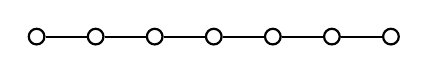
\begin{tikzpicture}[style=thick,scale=0.5] 
\tikzstyle{every node}=[circle,inner sep=2pt,draw] 
\node{\null}[grow'=right] 
child{node{\null} 
child{node{\null} 
child{node{\null}
child{node{\null}
child{node{\null}
child{node{\null}}}}}}};
\end{tikzpicture} 
&
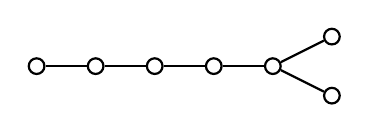
\begin{tikzpicture}[style=thick,scale=0.5] 
\tikzstyle{every node}=[circle,inner sep=2pt,draw] 
\node{\null}[grow'=right] 
child{node{\null} 
child{node{\null} 
child{node{\null}
child{node{\null}
child{node{\null}}
child{node{\null}}}}}};
\end{tikzpicture} 
\cr & \cr & \cr
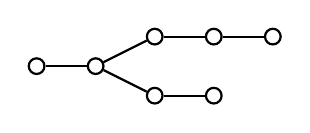
\begin{tikzpicture}[style=thick,scale=0.5] 
\tikzstyle{every node}=[circle,inner sep=2pt,draw] 
\node{\null}[grow'=right] 
child{node{\null} 
child{node{\null} 
child{node{\null}
child{node{\null}}}}
child{node{\null}
child{node{\null}}}};
\end{tikzpicture} 
&
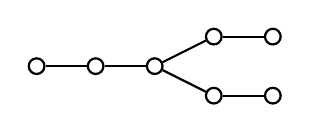
\begin{tikzpicture}[style=thick,scale=0.5] 
\tikzstyle{every node}=[circle,inner sep=2pt,draw] 
\node{\null}[grow'=right] 
child{node{\null} 
child{node{\null} 
child{node{\null}
child{node{\null}}}
child{node{\null}
child{node{\null}}}}};
\end{tikzpicture} 
\cr & \cr & \cr
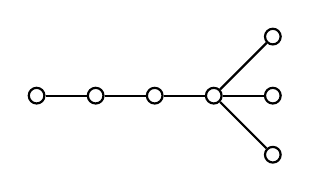
\begin{tikzpicture}[style=thick,scale=0.5] 
\tikzstyle{every node}=[circle,inner sep=2pt,draw] 
\node{\null}[grow'=right] 
child{node{\null} 
child{node{\null} 
child{node{\null}
child{node{\null}}
child{node{\null}}
child{node{\null}}}}};
\end{tikzpicture} 
&
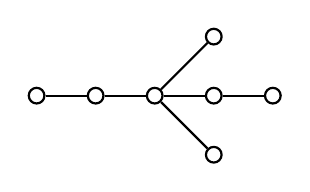
\begin{tikzpicture}[style=thick,scale=0.5] 
\tikzstyle{every node}=[circle,inner sep=2pt,draw] 
\node{\null}[grow'=right] 
child{node{\null} 
child{node{\null} 
child{node{\null}}
child{node{\null}
child{node{\null}}}
child{node{\null}}}};
\end{tikzpicture}
\cr & \cr & \cr
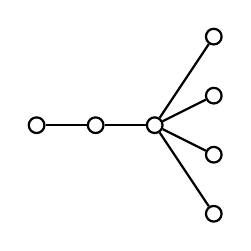
\begin{tikzpicture}[style=thick,scale=0.5] 
\tikzstyle{every node}=[circle,inner sep=2pt,draw] 
\node{\null}[grow'=right] 
child{node{\null} 
child{node{\null} 
child{node{\null}}
child{node{\null}}
child{node{\null}}
child{node{\null}}}};
\end{tikzpicture}
 &
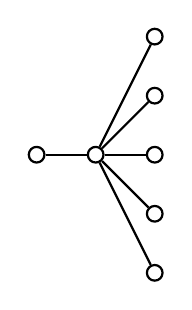
\begin{tikzpicture}[style=thick,scale=0.5] 
\tikzstyle{every node}=[circle,inner sep=2pt,draw] 
\node{\null}[grow'=right] 
child{node{\null} 
child{node{\null}} 
child{node{\null}}
child{node{\null}}
child{node{\null}}
child{node{\null}}};
\end{tikzpicture}
\cr & \cr & \cr
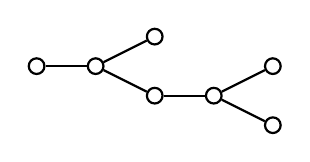
\begin{tikzpicture}[style=thick,scale=0.5] 
\tikzstyle{every node}=[circle,inner sep=2pt,draw] 
\node{\null}[grow'=right] 
child{node{\null} 
child{node{\null}} 
child{node{\null}
child{node{\null}
child{node{\null}}
child{node{\null}}}}};
\end{tikzpicture}
&
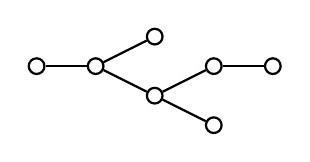
\begin{tikzpicture}[style=thick,scale=0.5] 
\tikzstyle{every node}=[circle,inner sep=2pt,draw] 
\node{\null}[grow'=right] 
child{node{\null} 
child{node{\null}} 
child{node{\null}
child{node{\null}
child{node{\null}}}
child{node{\null}}}};
\end{tikzpicture}
\cr & \cr & \cr
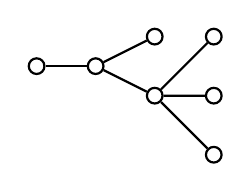
\begin{tikzpicture}[style=thick,scale=0.5] 
\tikzstyle{every node}=[circle,inner sep=2pt,draw] 
\node{\null}[grow'=right] 
child{node{\null} 
child{node{\null}} 
child{node{\null}
child{node{\null}}
child{node{\null}}
child{node{\null}}}};
\end{tikzpicture}
& 
\end{tabular}
\end{center}


\chapter{C08, 9. évfolyam}
\section{Szakkör}

\subsection*{2010.09.14. -- Pitagoraszi számhármasok}
\begin{enumerate}
\item Igazoljuk, hogy ha $m>n>0$ egészek, akkor
$x=m^2-n^2$, $y=2mn$, $z=m^2+n^2$ pitagoraszi számhármas ($x^2+y^2=z^2$).
\item Tegyük fel, hogy $m$ és $n$ szomszédos egészek. Mit mondhatunk $y$ és $z$
kapcsolatáról? Adjunk meg 6 egyszerű példát!
\item Válasszuk most $m$ és $n$ helyére az előző példabeli $y$-t és $x$-et. Mit tapasztalunk?
\item Válasszuk $m$ és $n$ értékének két egymást követő háromszögszámot. Mi lesz $x$ értéke?
\item Igazoljuk, hogy az 1. feladatban szereplő $x,y,z$ közül az egyik osztható 3-mal és egyik osztható 5-tel.
\item ($*$) Határozzuk meg az összes olyan $x,y,z$ pitagoraszi számhármast, amelyben $y=48$.
\end{enumerate}

\subsection*{2010.09.21. -- Számelméleti feladatok}
\begin{enumerate}
\item Soroljuk fel nagyság szerint növekvő sorrendben az összes 0-nál nagyobb,
1-nél kisebb,
\begin{abc2}
\item legfeljebb 5 nevezőjű;
\item legfeljebb 7 nevezőjű törtet.
\end{abc2}
\noindent (Farey-sorozatok)
\item Keressünk kapcsolatot az előző sorozatokban az egymást követő 3 tört között!
\item Hány tört van a 10-nél kisebb vagy egyenlő nevezőjű törtek Farey-sorozatában?
\item Ábrázoljuk az 1.a) feladatban szereplő Farey-törteket a következő pontokkal:
a $\dfrac{p}{q}$ törtnek a képe legyen a $(p;q)$ koordinátájú pont. Kössük össze a 
szomszédos törteknek megfelelő pontokat. A Farey-sorozatot kiegészíthetjük így: elé írjuk a $\dfrac{0}{1}$ törtet és a végére írjuk az $\dfrac{1}{1}$ törtet. Mit tapasztalunk?
\end{enumerate}



\underline{Érdekesség}: az $n$-edik Farey-sorozat elemeinek száma jó közelítéssel $\dfrac{3n^2}{\pi^2}$. Bizonyítás nehéz.

\subsection*{2010.09.28. -- Figurális számok és tulajdonságaik}
\begin{enumerate}
\item Adjunk képletet az $n$-edik háromszögszámra, ötszögszámra, hatszögszámra.
\item Adjunk meg képletet az első $n$ háromszögszám, négyzetszám, ötszögszám, hatszögszám összegére.
\item Igazoljuk, hogy két szomszédos háromszögszám összege négyzetszám.
\item Igazoljuk, hogy egy háromszögszám 8-szorosához 1-et adva négyzetszámot kapunk.
\item ($*$) Igazoljuk, hogy ha egy négyzetszám 8-szorosához 1-et adva négyzetszámot kapunk, akkor a kiindulásként vett négyzetszám háromszögszám is.
\item Értelmezzük a térbeli figurális számokat, az u.n. \underline{piramidális} számokat. Keressünk képletet!
\item Három egymást követő pozitív egész közül a középső teljes köb. Igazoljuk, hogy szorzatuk osztható 504-gyel. 
\end{enumerate}

\subsection*{2010.10.05. -- A kis-Fermat tétel és megfordítása}
\begin{enumerate}
\item ($*$) Igazoljuk teljes indukcióval ($a$-ra), hogy ha $p>0$, prím és $a>0$ egész, akkor $p\mid a^p-a$.\\ (,,kis-Fermat tétel'')
\item Mutassuk meg, hogy a megfordítás nem igaz. Érdekes, hogy ha $n>1$ és $n\mid 2^n-2$, akkor $1<n\le 300$-ig $n$ csak prím lehet. Igazoljuk, hogy bár $341\mid 2^{341}-2$, de 341 nem prímszám!
\item \underline{Definíció}: $n$ \underline{pszeudoprím}, ha $n>1$, $n\mid 2^n-2$
és $n$ összetett szám. Igazoljuk, hogy 2047 pszeudoprím.
\item Igazoljuk, hogy $161038=2\cdot 73\cdot 1103$ páros pszeudoprím. 
($161037=3^2\cdot 29\cdot 617$)
\item ($*$) Igazoljuk, hogy ha $n$ egy páratlan pszeudoprím, akkor $2^n-1$ is
(páratlan) pszeudoprím. Tehát végtelen sok páratlan pszeudoprím van.
\end{enumerate}

\subsection*{2010.10.12. -- Kombinatorika feladatok}
\begin{enumerate}
\item A $8\times 8$-as sakktáblán egy átló két végén álló mezőt kivágjuk. Lefedhető-e a megmaradt 62 mező hézagmentesen és egyrétűen 31 dominóval?
\item A $8\times 8$-as sakktábláról kivágunk egy fehér és egy fekete mezőt. Igazoljuk, hogy a megmaradt 62 mező mindig lefedhető egyrétűen és hézagtalanul 31 dominóval.
\item A A $8\times 8$-as sakktábla összes mezőjét futókkal akarjuk ,,lefogni''.
Legkevesebb hány futóra van ehhez szükség?
\item Egy $6\times 6$-os ,,sakktáblát'' ($2\times 1$-es) dominóval lefedtünk hézagmentesen és egyrétűen. Mutassuk meg, hogy akkor lehet olyan egyenes ,,utat''
találni a sakktáblán, amely mentén egyetlen dominót sem ,,vágunk ketté''.
\item ($*$) Igazoljuk, hogy minden poliédernek (síklapokkal határolt testnek) van legalább 2 azonos oldalszámú lapja.
\item Egy konvex $n$-szög belsejében felvettünk $k$ pontot és ezeket egymással és a sokszög csúcsaival összekötöttük úgy, hogy a sokszöget háromszögekre bontottuk és a szakaszok csak a csúcsokban és a felvett pontokban metszhetik egymást. Hány háromszöget kaptunk?
\end{enumerate}

\subsection*{2010.10.26. -- Algebra feladatok}
\begin{enumerate}
\item Igazoljuk, hogy ha $x,y,z\in\mathbb{R}$, akkor
$x^2+y^2+z^2\ge xy+xz+yz$.
\item Bizonyítsuk be, hogy ha $x+y+z=a$, akkor $x^2+y^2+z^2\ge \dfrac{a^2}{3}$,
ahol $x,y,z,a\in\mathbb{R}$.
\item Mutassuk meg, hogy ha $a,b>0$ és $a+b=1$, akkor
$$\left(a+\dfrac{1}{a}\right)^2+\left(b+\dfrac{1}{b}\right)^2\ge \dfrac{25}{2}.$$
\item Igazoljuk, hogy ha $a,b,c$ egy háromszög három oldalának mérőszáma, akkor 
$$abc\ge (a+b-c)(a+c-b)(b+c-a).$$
\item Igazoljuk, hogy ha $a,b,c>0$ valós számok, akkor $\dfrac{a^3+b^3}{2}\ge 
\left(\dfrac{a+b}{2}\right)^3$.
\item ($*$) Igazoljuk, hogy ha $a,b,c,d\in\mathbb{R}$ és 
$a^2+b^2=1$, $c^2+d^2=1$, akkor $ac+bd\le 1$.
\end{enumerate}

\subsection*{2010.11.09. -- Kombinatorika feladatok}
\begin{enumerate}
\item Adott $n$ darab pozitív egész szám. Igazoljuk, hogy kiválasztható közülük néhány úgy, hogy ezek összege osztható $n$-nel.
\item Igaz-e, hogy minden $k>0$ egész számnak van olyan többszöröse, amelynek a 
tízes számrendszerbeli alakja csak 0 és 1 számjegyet tartalmaz.
\item Adott a síkon öt rácspont (mindkét koordinátája egész). Igazoljuk, hogy ezek között van kettő, amelyek felezőpontja is rácspont.
\item Egy egységnyi oldalhosszúságú négyzetben kijelölünk 5 pontot. Igazoljuk, hogy ezek között van kettő, amelyek távolsága nem nagyobb $\dfrac{\sqrt 2}{2}$-nél.
\item 5 párhuzamost egyenest az előzőkre merőleges, szintén egymással párhuzamos 11 egyenes metsz. Hány téglalapot határoznak meg ezek az egyenesek?
\item ($*$) Igazoljuk, hogy az olyan páratlan szám, amely $n$ darab különböző prímszám szorzata, $2^{n-1}$-féleképpen írható fel két négyzetszám különbségeként.
\end{enumerate}

\subsection*{2010.11.16. -- Versenyfeladatok geometriából}
\begin{enumerate}
\item Az $ABCD$ trapéz $AD$ alapján fekvő szögek összege $90^\circ$. Igazoljuk, hogy a két alap felezőpontját összekötő szakasz hossza az alapok különbségének fele.
\item Igazoljuk, hogy ha az $ABCD$ trapéz két párhuzamos oldala $AD$ és $BC$, akkor $$AC^2+BD^2=AB^2+CD^2+2\cdot AD\cdot BC.$$
\item Három egyenlő sugarú kör egy pontban metszi egymást. Két kör másik metszéspontja és a harmadik kör középpontja meghatároz egy egyeneset. Igazoljuk, hogy az így kapott három egyenes egy ponton halad át.
\item Igazoljuk, hogy egy derékszögű háromszögben a befogók összege egyenlő a háromszögbe írt és a háromszög köré írt körök átmérőinek összegével.
\item Igazoljuk, hogy egy derékszögű háromszögben a derékszög felezője felezi a derékszög csúcsából induló magasságvonal és súlyvonal szögét is.
\end{enumerate}

\subsection*{2010.11.30. -- Versenyfeladatok}
\begin{enumerate}
\item Igazoljuk, hogy ha $p>3$ és $p$ prímszám, akkor $p$ vagy $6k-1$, vagy $6k+1$
alakú.
\item Mutassuk meg, hogy ha két pozitív egész szám különbsége 2, akkor a köbeik különbsége előállítható három négyzetszám összegeként.
\item Igazoljuk, hogy ha $x$ egész szám, akkor $5x^2+6x+15$ nem teljes négyzet.
\item ($*$) Oldjuk meg az egész számok halmazán a következő egyenletet: $x^3-13xy+y^3=13$.
\item Oldjuk meg az egész számok halmazán a következő egyenletet: $2xy-3x-3y-5=0$.
\end{enumerate}

\subsection*{2010.12.07. -- Versenyfeladatok}
\begin{enumerate}
\item Két kör belülről érinti egymást az $A$ pontban. A nagyobb kör átmérője $AB$,
a nagyobb kör $BK$ húrja a $C$ pontban érinti a kisebb kört. Igazoljuk, hogy $AC$ az $ABK$ háromszög szögfelezője.
\item Az $ABC$ egyenlőszárú háromszög $AB$ alapján van a $D$ pont. Tudjuk, hogy
$AD=a$ és $DB=b$ ($a<b$). Az $ACD$ háromszögbe írt kör a $P$, a $BCD$ háromszögbe írt kör a $Q$ pontban érinti a $CD$ szakaszt. Határozzuk meg a $PQ$ távolságot.
\item Egy derékszögű trapézban az átlók merőlegesek egymásra. A trapéz két párhuzamos oldalának aránya $k$. Határozzuk meg a trapéz átlóinak arányát.
\item Az $ABCD$ trapéz $AB$ alapja $a$, $CD$ alapja $b$, ($a<b$). Az $A,B$ és $C$ csúcsokra illeszkedő kör érinti az $AD$ oldalt. Határozzuk meg az $AC$ átlót.
\item Egy $R$ és egy $r$ sugarú kör belülről érinti egymást. Határozzuk meg annak a körnek a sugarát, amely érinti mindkét kört és a közös átmérőjüket.
\end{enumerate}

\subsection*{2010.12.14. -- Vegyes feladatok}
\begin{enumerate}
\item Egy derékszögű háromszög átfogójának két végpontja egy derékszög két szárán mozog. Mit ír le eközben a háromszög derékszögű csúcsa?
\item Igazoljuk, hogy minden $\overline{abcabc}$ alakú szám ($a,b,c$ számjegyek)
osztható 143-mal.
\item Oldjuk meg az egész számok halmazán a következő egyenletrendszert:
\begin{align*}
x^2&=y^2+z^2+1;\cr
x&=y+z-3.
\end{align*}
\item ($*$) Igazoljuk, hogy a $\left(\sqrt{2}-1\right)^{2010}=\sqrt{k}-\sqrt{k-1}$
egyenlet megoldható a pozitív egészek halmazán.
\item Melyik az a legkisebb pozitív egész szám, amelyre igaz, hogy ha az utolsó 
számjegyét, a 4-et első helyre visszük (a többi számjegy nem változik), akkor a szám 4-szeresét kapjuk?
\end{enumerate}

\subsection*{2011.01.04. -- Versenyfeladatok}
\begin{enumerate}
\item Jelölje $P(n)$ az $n$ tízes számrendszerben felírt alakjában a számjegyek szorzatát. Számítsuk ki a következő összeget:
$$P(1000)+P(1001)+P(1002)+\ldots+P(2000).$$
\item Van-e olyan $n>0$ egész szám, hogy az
$$n+1, 2n+1, 3n+1, 4n+1, \ldots$$
sorozatban nincs egyetlen köbszám sem?
\item ($*$) Az $a,b,c,d$ pozitív számokra teljesül: $\dfrac{a+b}{c+d}<2$.
Igazoljuk, hogy $\dfrac{a^2+b^2}{c^2+d^2}<8$.
\item El lehet-e helyezni az első 8 pozitív egész számot egy kör kerületén úgy, hogy bármely szám osztható legyen két szomszédja különbségének abszolút értékével?
\item ($*$) Melyik az a pozitív egész szám, amely 100-szorosa az osztói számának?
\end{enumerate}

\subsection*{2011.01.11. -- Versenyfeladatok}
\begin{enumerate}
\item Van-e olyan $n>0$ egész szám, amelyre $n^2+n+1$ osztható 9-cel?
\item Leírtunk egymást követő 500 pozitív egész számot és így összesen 1999 számjegyet írtunk le. Melyik volt ez az 500 szám?
\item Az $1!\cdot 2!\cdot 3!\cdot \ldots \cdot 99!\cdot 100!$ szorzatból egyetlen 
$k!$ alakú tényezőt kell kihagyni, hogy a megmaradók szorzata négyzetszám legyen.
Melyik ez a tényező?
\item ($*$) Adjuk meg az összes olyan pozitív egész $n$ számot, amely előállítható
$n-1$ három különböző pozitív osztójának összegeként.
\item Oldjuk  meg a valós számok halmazán a következő egyenletrendszert:
$$x=\dfrac{\sqrt{yz}}{y+z},\qquad
y=\dfrac{\sqrt{zx}}{z+x},\qquad
z=\dfrac{\sqrt{xy}}{x+y}.
$$
\end{enumerate}

\subsection*{2011.01.18. -- Versenyfeladatok}
\begin{enumerate}
\item Számítsuk ki az első $n$ háromszögszám reciprokának összegét.
\item Igazoljuk, hogy minden háromszögszám felírható két kisebb háromszögszám és egy négyzetszám összegeként.
\item Milyen számjegyre végződhetnek a háromszögszámok?
\item Egy hatjegyű, tízes számrendszerben felírt $\overline{abbabb}$ alakú
szám hat egymást követő prímszám szorzata. Melyik ez a hatjegyű szám?
\item Az $a$ és $b$ számjegyek, $a\ne 0$. Igazoljuk, hogy az $\overline{ababab}$
alakú hatjegyű számok oszthatók 777-tel.
\item Melyik az a háromjegyű tízes számrendszerbeli szám, amely számjegyei összegének 17-szerese?
\end{enumerate}

\subsection*{2011.02.01.}
\begin{enumerate}
\item Adott térfogatú téglatestek közül melyiknek legkisebb a felszíne?
\item Igazoljuk, hogy ha $b,d>0$ és $\dfrac{a}{b}\le \dfrac{c}{d}$, akkor
$$\dfrac{a}{b}\le\dfrac{a+c}{b+d}\le\dfrac{c}{d}.$$
\item Igazoljuk, hogy ha $a>0$ és $\dfrac{1}{x^2}+\dfrac{1}{y^2}=a$, akkor
$x^2+y^2\ge\dfrac{4}{a}$.
\item Igazoljuk, hogy ha $x,y,z\in\mathbb{R}$ és $x+y+z=5$, $xy+yz+xz=8$, akkor
$1\le x\le \dfrac{7}{3}$.
\item Igazoljuk, hogy ha $a,b,c>0$, akkor $\dfrac{ab}{c}+\dfrac{bc}{a}+\dfrac{ac}{b}\ge a+b+c$.
\item ($*$) Igazoljuk, hogy ha $a,b,c>0$ és $a^2+b^2=c^2$, akkor $a^3+b^3<c^3$.
\end{enumerate}

\subsection*{2011.02.22.}
\begin{enumerate}
\item Melyik az a legkisebb 36-tal osztható tízes számrendszerbeli szám, amelynek számjegyei közt csak 0 és 1 szerepel?
\item Oldjuk meg a valós számok halmazán: $3x^2-6x+16=(x^2-2x+2)^2$.
\item Az $ABC$ hegyesszögű háromszögben az $A$ csúcsnál $30^\circ$-os szög van. $B_1$ az $AC$, $C_1$ az $AB$ oldal felezőpontja, $B_2$ a $B$-ből, $C_2$ a $C$-ből húzott magasság talppontja. Igazoljuk, hogy a $B_1C_2$ egyenes merőleges a $B_2C_1$ egyenesre.
\item A $p$ valós paraméter mely értékeire igaz minden valós $x$-re a következő egyenlőtlenség: $\dfrac{2x^2+2x+3}{x^2+x+1}\le p$?
\item Határozzuk meg az összes olyan $p$ és $q$ prímszámot, amelyekre $7p+q$ és 
$pq+11$ is prím!
\item Egy derékszögű háromszög oldalainak hosszai egész számok. Igazoljuk, hogy a háromszög három egyenlő területű háromszögre darabolható úgy, hogy a részek területe is egész szám!
\end{enumerate}

\subsection*{2011.03.01.}
\begin{enumerate}
\item Melyek azok a pozitív egész $n$ számok, amelyekre $\dfrac{n+11}{n-9}$ is pozitív egész?
\item Valaki 1981-ben annyi éves, mint születési évszáma számjegyeinek összege. Mikor született?
\item Oldjuk meg a valós számok halmazán: 
$\left| 1+\left|\dfrac{x-4}{5}\right|-x\right|>3$.
\item Igazoljuk, hogy ha $p$ és $p^2+8$ is prím, akkor $p^2+p+1$ is prím.
\item Egy háromszög kerülete 19 egység, oldalainak hossza egész számokkal fejezhető ki és egyik oldalának hossza a másik kettő szorzatával egyenlő. Mekkorák az oldalak?
\item Három pozitív egész szám összege ugyanannyi, mint a szorzatuk. Melyek lehetnek ezek a számok?
\end{enumerate}

\subsection*{2011.03.08.}
\begin{enumerate}
\item Oldjuk meg a valós számok halmazán: $(x+1)^4+(x+3)^4=16$.
\item Számítsuk ki a következő összeget:
$$1+2-3+4+5-6+7+8-9+\ldots+3n-2+3n-1-3n.$$
\item Határozzuk meg a következő függvény legnagyobb értékét:$f(x)=\dfrac{3x^2+6x+7}{x^2+2x+2},\quad x\in\mathbb{R}$.
\item Adott egy derékszögű háromszög, befogóinak hossza 1 és 2 egység. Tükrözzük a háromszög mindegyik csúcsára a másik két csúcsát. Számítsuk ki a kapott hat tükörkép által meghatározott hatszög területét.
\item Egy mértani sorozat három szomszédos elemének összege 62, a középső elem 10. 
Melyik ez a három szám?
\item Igazoljuk, hogy h $x,y,z>0$ valós számok, akkor teljesül a következő egyenlőtlenség:
$$\dfrac{xy}{x+y}+\dfrac{yz}{y+z}+\dfrac{zx}{z+x}\le\dfrac{x+y+z}{2}.$$
\end{enumerate}

\subsection*{2011.03.22.}
\begin{enumerate}
\item Hány 0-ra végződik $200!$\, ?
\item Osztható-e 7-tel $\binom{2000}{1000}$\, ?
\item Számítsuk ki a következő összeget:
$$\dfrac{1}{1+2}+\dfrac{1}{1+2+3}+\dfrac{1}{1+2+3+4}+\ldots+\dfrac{1}{1+2+3+\ldots+n}.$$
\item Igazoljuk, hogy ha két pozitív egész szám különbsége 2, akkor köbeik különbsége előállítható három négyzetszám összegeként.
\item ($*$) Igazoljuk, hogy $\ctg 70^\circ+4\cos 70^\circ=\sqrt{3}$.
\item ($*$) Határozzuk meg az összes olyan pozitív egész $m,n$ számot, amelyre teljesül, hogy $n\mid 2m-1$ és $m\mid 2n-1$.
\end{enumerate}

\subsection*{2011.05.17.}
\begin{enumerate}
\item Oldjuk meg a valós számok halmazán:
\begin{abc}
\item $\sqrt[3]{x-1}+\sqrt[3]{x+1}=x\sqrt[3]{2}$;
\item $\sqrt{x-4a+16}=2\sqrt{x-2a+4}-\sqrt{x}$;
\item $\dfrac{(x^2-4)(x^3-1)}{x^2-2x+3}>0$.
\end{abc}
\item Igazoljuk, hogy ha $n>1$ egész, akkor
$$\dfrac{1}{2^2}+\dfrac{1}{3^2}+\ldots+\dfrac{1}{n^2}<\dfrac{n-1}{n}.$$
\item Oldjuk meg a valós számok halmazán: $\dfrac{1-\sqrt{1-4x^2}}{x}<3$.
\item Oldjuk meg a valós számok halmazán:
\begin{abc}
\item ($*$) $\cos 3x\cos^3 x+\sin 3x\sin^3 x=0$;
\item $\tg\frac{x}{2}>\dfrac{\tg x-2}{\tg x+2}$.
\end{abc}
\end{enumerate}

\subsection*{2011.05.24.}
\begin{enumerate}
\item Igazoljuk, hogy ha $\alpha, \beta, \gamma$ egy hegyesszögű háromszög szögei, akkor $2<\sin^2 \alpha+\sin^2\beta+\sin^2\gamma\le\dfrac{9}{4}$.
\item ($*$) Oldjuk meg a valós számok halmazán: $\sqrt[3]{25x(2x^2+8)}=4x+\dfrac{3}{x}$.
\item Egy háromszög oldalainak hossza 13, 12, 5 egység. Hány olyan pont van a háromszög belsejében, amelynek az oldalaktól mért távolságai pozitív egész számú egységek? Mekkorák ezek a távolságok?
\item Oldjuk meg az egész számok halmazán:
\begin{align*}
x^2+xy-y^2&= 1,\cr
y^2-xy+x&=1.
\end{align*}
\end{enumerate}

\subsection*{2011.05.31.}
\begin{enumerate}
\item Oldjuk meg a valós számok halmazán a következő egyenletet:
$$2\sqrt{x+y}+3\sqrt{10-x}+2\sqrt{7-y}=17.$$
\item Határozzuk meg az $n^5-5n^3+4n+1,\quad n>0$ egész szám utolsó számjegyét.
\item Hány megoldása van a $[0;2\pi]$ intervallumban a $\sin 2010x=\sin 2011x$
egyenletnek?
\item Igazoljuk, hogy ha $n>0$ egész, akkor
$$\sqrt{1+\frac{1}{2}}+
\sqrt{1+\frac{1}{2^2}}+\ldots+
\sqrt{1+\frac{1}{2^n}}<n+\frac{1}{2}.
$$
\item ($*$) Számítsuk ki $\dfrac{\tg 20^\circ+4\sin 20^\circ}{\ctg 10^\circ-4\cos 10^\circ}$ pontos értékét.
\end{enumerate}

\section{Sorozatok}

\subsection*{2010.09.02. -- Bemelegítő feladatok}
\begin{enumerate}
\item Oldjuk meg az egész számok halmazán: 
$\sqrt{n+\sqrt{n+\ldots+\sqrt{n+\sqrt{n}}}}=k$.
\item ($*$) Oldjuk meg a valós számok halmazán:
$2x^3=(3x^2-x-1)\sqrt{1+x}$.
\item ($*$) Határozzuk meg az
$f(x)=\sqrt{x^2-6x+13}+\sqrt{x^2-14x+58}, x\in\mathbb{R}$ függvény legkisebb értékét.
\item Igazoljuk, hogy
\begin{abc2}
\item $\sqrt{6+\sqrt{6+\sqrt{6+\sqrt{6+\sqrt{3}}}}}<3$;
\item $\frac{2-\sqrt{2+\sqrt{2+\sqrt{2+\sqrt{2}}}}}{2-\sqrt{2+\sqrt{2+\sqrt{2}}}}>\frac{1}{4}$.
\end{abc2}
\item ($*$) Tudjuk, hogy $x,y,z>0$ és $x+y+z=1$. Határozzuk meg 
$\sqrt{1+x^2}+\sqrt{1+y^2}+\sqrt{1+z^2}$ legkisebb értékét.
\end{enumerate}

\subsection*{2010.09.07. -- Sorozatok és tulajdonságaik}
\begin{enumerate}
\item Számítsuk ki a kétjegyű páros számok összegét.
\item Adott a következő sorozat: $a_n=2^n, (n=0,1,2,\ldots)$. Számítsuk ki a sorozat első $n$ tagjának összegét!
\item Az $a_n=\left(\frac{1}{2}\right)^n$ sorozat ($n=0,1,2,\ldots$) első $n$ tagjának számítsuk ki az összegét!
\item Egy sorozat első tagja 10, minden további tag 3-mal nagyobb az előző tagnál. Számítsuk ki a sorozat
\begin{abc2}
\item első 100;
\item első $n$
\end{abc2}
tagjának összegét.
\item Egy sorozat első tagja 3, minden további tag az előző tag kétszerese. Számítsuk ki a sorozat
\begin{abc2}
\item első 100;
\item első $n$
\end{abc2}
tagjának összegét.
\item Egy sorozat első tagja $a_1$, minden további tag $d$-vel nagyobb az előző tagnál. Számítsuk ki az első $n$ tag összegét és a sorozat $n$-edik tagját.
\end{enumerate}

\subsection*{2010.09.08.}
\begin{enumerate}
\item Egy sorozat első tagja $a_1$, minden további tag az előző tag $q$-szorosa. Számítsuk ki a sorozat $n$-edik tagját és első $n$ tagjának összegét (mértani sorozat).
\item Az $a_n$ sorozat definíciója:
$$a_1=1,\quad a_{n+1}=\frac{1}{1+a_n}.$$
Vizsgáljuk meg, hogyan viselkedik a sorozat a növekedés és fogyás szempontjából.
\item Keressünk olyan mértani sorozatot, amelyre teljesül, hogy $a_{n+2}=a_n+a_{n+1}$.
\item Az $1,4,10,19,\ldots$ sorozat szomszédos tagjainak különbségéből álló sorozat egy számtani sorozat. Adjuk meg a sorozat $n$-edik tagját és első $n$ tagjának összegét.
\item Számítsuk ki a következő összeget:
$$\frac{1}{2}+\frac{3}{2^2}+\frac{5}{2^3}+\ldots
+\frac{2n-1}{2^n}.$$
\item Számítsuk ki:
$$1+2x+3x^2+\ldots+(n+1)x^n.$$
\end{enumerate}


\subsection*{2010.09.09.}
\begin{enumerate}
\item Az $(a_n)$ sorozat definíciója: $a_1=1, a_2=2$ és ha $n\ge 1$, akkor $a_{n+2}=3a_{n+1}-2a_n$. Fejezzük ki $a_n$-et $n$-nel.
\item Igazoljuk, hogy az $a_1=2$, $a_{n+1}=\frac{1}{2}\left(a_n+\frac{1}{a_n}\right)$ sorozat monoton fogyó és alulról korlátos. Szemléltessük a sorozat elemeit az 
$$f(x)=\frac{1}{2}\left(x+\frac{1}{x}\right)$$
függvény grafikonjával.
\item Egy számtani sorozatról a következőket tudjuk:
\begin{align*}
a_2+a_4+a_6&=36;\cr
a_2a_3&=54.
\end{align*}
Számítsuk ki a sorozat első tagját és különbségét.
\item Egy számtani sorozat három egymást követő elemének összege 3, a három egymást követő elem köbének összege 15. Számítsuk ki a számtani sorozat differenciáját.
\item Számítsuk ki minél egyszerűbben a következő összeget:
$$100^2-99^2+98^2-97^2+\ldots+2^2-1^2.$$
\end{enumerate}


\subsection*{2010.09.15.}
\begin{enumerate}
\item Egy mértani sorozatnál tudjuk, hogy 
$$a_1+a_2=4\text{~és~}a_5a_2=6.$$
Számítsuk ki a sorozat első elemét és hányadosát.
\item Egy számtani sorozat első három elemének összege 9. Ha az első elemből 4-et elveszünk, a másodikhoz 1-et, a harmadikhoz 15-öt hozzáadunk, akkor egy mértani sorozat első három elemét kapjuk. Melyik a számtani sorozat első három eleme?
\item Számítsuk ki azoknak a kétjegyű pozitív egész számoknak az összegét, amelyek 3-mal osztva 2-t adnak maradékul.
\item Igazoljuk, az $x^2-yz$, $y^2-zx$, $z^2-xy$ számok egy számtani sorozat első három elemét adják, ha $x,y,z$ egy számtani sorozat első három eleme.
\item Egy mértani sorozatban $a_1-a_2=8$, $a_2+a_3=12$. Számítsuk ki a sorozat első tagját és hányadosát.
\item Egy mértani sorozatban $a_1=3$, $a_{10}=1536$. Számítsuk ki $q$-t és $s_{10}$-et.
\item Igazoljuk, hogy ha $x,y,z$ egy mértani sorozat első három eleme, akkor 
$x^3+2xy^2+y^2z$,
$x^2y+y^3+xyz+yz^2$ és 
$xy^2+2y^2z+z^3$ is egy mértani három egymást követő eleme.
\end{enumerate}


\subsection*{2010.09.16.}
\begin{enumerate}
\item Egy szabályos háromszög oldala 2 egység. A háromszögbe egyenlő sugarú köröket írunk úgy, hogy érintik egymást és a háromszög oldalait. Egy-egy háromszögoldalt $n$ kör érint. Számítsuk ki a körök sugarát és területének összegét.
\item Számítsuk ki ki:
\begin{abc}
\item $\frac{1^2+3^2+5^2+\ldots+(2n-1)^2}{2^2+4^2+6^2+\ldots+(2n)^2}$;
\item $\frac{1^3+^3+3^3+\ldots+n^3}{n^3}-\frac{n}{4}$;
\item $(1+x)(1+x^2)(1+x^4)\ldots(1+x^{2^n})$.
\end{abc}
\item Vizsgáljuk a következő sorozatot:
$a_1=\frac{x}{2}$, ahol $0<x<1$; $a_{n+1}=\frac{x}{2}+\frac{a_n^2}{2}$. Igazoljuk, hogy $a_n<1$ minden $n$-re és $a_{n+1}>a_n$ szintén minden $n$-re igaz.

\item Igazoljuk, hogy az $a_1=\sqrt 2$, $a_{n+1}=\sqrt{2+a_n}$ sorozat növekvő, de felülről korlátos, azaz van olyan szám, aminél a sorozat minden eleme kisebb.
\end{enumerate}


\subsection*{2010.09.21.}
\begin{enumerate}
\item Az $1,4,10,19,\ldots$ sorozat szomszédos tagjainak különbsége számtani sorozatot alkot. Számítsuk ki a sorozat 100. tagját és az első 100 tag összegét.
\item Számítsuk ki az
$$1,3,6,10,\ldots,\frac{n(n+1)}{2},\ldots$$
sorozat első 200 tagjának összegét.
\item Adott két számtani sorozat: az egyik
$17,21,25,\ldots$, a másik $16,21,26,\ldots$. A két sorozatban vannak közös elemek is. Számítsuk ki a két sorozat első 100 közös elemének összegét.
\item ($*$) Egy számtani sorozatról tudjuk, hogy a negyedik tagja 4. A sorozat $d$ különbségének mely értékére igaz, hogy a sorozat első három tagjának páronként vett szorzatát összeadva a legkisebb értéket kapjuk?
\item Számítsuk ki a következő összeg értékét:
$$\frac{1}{1\cdot 3}+\frac{1}{3\cdot 5}
+\frac{1}{5\cdot 7}+\ldots+\frac{1}{999\cdot 1001}.$$
\end{enumerate}


\subsection*{2010.09.23.}
\begin{enumerate}
\item Valaki január 1-én 100~000~Ft-ot tesz egy bankba évi 6\%-os kamatra. Kamatos kamattal 6 év alatt hány forintra nő a betét?
\item Évi 5\%-os kamat esetén 6 év alatt 80~000~Ft hány forintra növekszik?
\item Igazoljuk a számtani sorozat következő tulajdonságát:
$$a_n=\frac{a_{n-k}+a_{n+k}}{2},$$
ha $n>k>0$ egészek.
\item Igazoljuk a mértani sorozat következő tulajdonságát:
$$\sqrt{a_{n-k}\cdot a_{n+k}}=a_n,$$
ha $a_1>0$, $q>0$ és $n>k>0$ egészek.
\item Igazoljuk a Fibonacci-sorozat következő tulajdonságait:
\begin{abc}
\item $f_1^2+f_2^2+\ldots+f_n^2=f_n\cdot f_{n+1}$;
\item $f_n^2-f_{n-1}\cdot f_{n+1}=(-1)^{n-1}$;
\item $f_{n-1}^2+f_n^2=f_{2n-1}$.
\end{abc}
\end{enumerate}


\subsection*{2010.09.28.}
\begin{enumerate}
\item Egy vállalatnál azt tervezik, hogy 5 éven keresztül évente 10\%-kal növelik a termelést. Hány \%-kal kell évente növelni a termelést, ha már a 4. év végére el akarják érni a tervezett végeredményt?
\item Négy szám egy számtani sorozat négy szomszédos eleme. Ha sorra 5-tel, 6-tal, 9-cel, 15-tel növeljük ezeket a számokat, akkor egy mértani sorozat négy szomszédos elemét kapjuk. Melyik ez a négy szám?
\item Három szám egy mértani sorozat három szomszédos eleme. Ha a középső számot 10-zel növeljük, akkor egy számtani sorozat három szomszédos elemét kapjuk. Melyik ez a három szám?
\item Négy szám egy mértani sorozat négy szomszédos eleme. A sorozat két szélső tagjának összege 14, a két középső tag összege 6. Melyik ez a négy szám?
\item Egy mértani sorozatban $a_6+a_5=48$ és $a_7-a_5=48$. Az elejétől kezdve hány tagot kell összeadni, hogy 1023-at kapjunk?
\item Egy mértani sorozat második eleme 20, első három elemének összege 70. Határozzuk meg a sorozat hatodik elemét!
\end{enumerate}


\subsection*{2010.09.29.}
\begin{enumerate}
\item Három szám egy mértani sorozat három szomszédos eleme, összegük 26. Ha az elsőhöz 1-et, a másodikhoz 6-ot, a harmadikhoz 3-mat adunk, akkor egy számtani sorozat három szomszédos tagját kapjuk. Mik lesznek a számtani sorozat tagjai?
\item Három szám egy mértani sorozat három szomszédos eleme. Ha a harmadik számból 64-et kivonunk, akkor a kapott számok egy számtani sorozat szomszédos tagjai. Ha most a középső számból vonunk ki 8-cat, akkor ismét egy mértani sorozat három szomszédos tagját kapjuk. Melyik volt az eredeti három szám?
\item Adjuk meg azt a számtani sorozatot, amelyben
$s_n=3n^2$.
\item Melyik az a mértani sorozat, amelyben az első és a negyedik tag összege 35, a második és harmadik tag összege 30?
\item Egy mértani sorozatban
\begin{align*}
a_1+a_2+a_3+a_4+a_5&=31,\cr
a_2+a_3+a_4+a_5+a_6&=62.
\end{align*}
Mennyi $a_1$ és $q$ értéke?
\item Igazoljuk, hogy ha $a$, $x$ tetszőleges valós számok, akkor
$(a+x)^2$, $a^2+x^2$, $(a-x)^2$ egy számtani sorozat első három eleme. Határozzuk meg ennek a sorozatnak az első $n$ tagjának összegét.
\end{enumerate}


\subsection*{2010.09.30.}
\begin{enumerate}
\item Oldjuk meg a következő egyenleteket:
\begin{abc}
\item $1+4+7+\ldots+x=117$;
\item $(x+1)+(x+4)+(x+7)+\ldots+(x+28)=155$.
\end{abc}
A bal oldalon számtani sorozatok összege áll.
\item Egy számtani sorozat első $n$ elemének összege
\begin{abc2}
\item $3n^2$;
\item $5n^2+3n$.
\end{abc2}
Határozzuk meg a sorozat első három elemét.
\item Igazoljuk, hogy ha $a,b,c$ egy számtani sorozat első három eleme, akkor
$$3(a^2+b^2+c^2)=6(a-b)^2+(a+b+c)^2.$$
\item Készítsünk olyan képletet, amelynek segítségével kiszámíthatjuk egy mértani sorozat első $n$ elemének szorzatát.
\item Három szám egy mértani sorozat első három eleme. A három szám összege 26, négyzetük összege 364. Melyek ezek a számok?
\end{enumerate}


\subsection*{2010.10.05. -- Ismétlő feladatok}
\begin{enumerate}
\item Igazoljuk, hogy az $a_1=\sqrt{a}$, $a_{n+1}=\sqrt{a+a_n}\quad(a>0)$ sorozat növekszik és felülről korlátos.
\item Három egész szám, amelyek összege 60, egy számtani sorozat három egymást követő tagja.
Ha ezekhez a számokhoz sorra $2{,}2$-et, $4$-et és $7$-et adunk, akkor a kapott számok egy mértani sorozat szomszédos tagjai. Melyik ez a három szám?

\item Számítsuk ki azoknak a háromjegyű pozitív egész számoknak az összegét, amelyeknek minden számjegye páros.
\item Egy számtani sorozat első tagja $a$, különbsége $d$. A $d$ mely értékére igaz, hogy $a_1a_3+a_2a_4$ értéke a lehető legkisebb?
\item Számítsuk ki a 30-cal osztható négyjegyű számok összegét.
\end{enumerate}


\subsection*{2010.10.06.}
\begin{enumerate}
\item Az $1,2,4,7,11,\ldots$ sorozat szomszédos tagjainak különbségei számtani sorozatot alkotnak. Számítsuk ki a sorozat $n$-edik tagját és első $n$ tagjának összegét.
\item Egy mértani sorozat első két tagjának összege 3, az első két tag négyzetének összege 5. Számítsuk ki a sorozat első tagját és hányadosát.
\item Az $a_n$ sorozat definíciója: $a_1=2$ és 
$a_{n+1}=3a_n+1$. Számítsuk ki a sorozat első $n$ tagjának összegét.
\item Számítsuk ki a következő összegeket:
\begin{abc}
\item $\frac{1}{1\cdot 5}+\frac{1}{5\cdot 9}
+\frac{1}{9\cdot 13}+\ldots+\frac{1}{(4n-3)\cdot(4n+1)}$;
\item $1+2\cdot 2+3\cdot 2^2+4\cdot 2^3+\ldots+
n\cdot 2^{n-1}$.
\end{abc}
\item Végezzük el a négyzetre emeléseket és adjuk össze:
$$
\left(x+\frac{1}{x}\right)^2+
\left(x^2+\frac{1}{x^2}\right)^2+
\ldots
+\left(x^n+\frac{1}{x^n}\right)^2.
$$
\end{enumerate}


\subsection*{2010.10.12.}
\begin{enumerate}
\item Egy számtani sorozat minden tagja pozitív egész szám. A második tag 12 és az első kilenc tag összege 200-nál nagyobb, de 220-nál kisebb. Adjuk meg a sorozatot.
\item Egy mértani sorozat első három tagjának összege 31, az első és a harmadik tag összege 26. Számítsuk ki a sorozat első tagját és hányadosát.
\item Három szám egy mértani sorozat három egymást követő tagja, szorzatuk 64, számtani közepük $\frac{14}{3}$. Melyik ez a három szám?
\item Adott 4 szám, az első három egy mértani, az utolsó három egy számtani sorozat első három eleme. Az első és a negyedik szám összege 21, a két középső összege 18. Melyik ez a négy szám?
\item Egy mértani sorozat első három tagjának összege 13, az első három tag négyzetének összege 91. Határozzuk meg a sorozatot.
\end{enumerate}


\subsection*{2010.10.13.}
\begin{enumerate}
\item Adott az $a_1=\frac{1}{4}$, $a_{n+1}=a_n(1-a_n)$, $n\ge 1$ sorozat. Igazoljuk, hogy $a_n\ge a_{n+1}$ és $a_n>0$ minden $n$-re. Ábrázoljuk a sorozat tagjait az $f(x)=x(1-x)$ függvény segítségével.
\item Egy mértani sorozat első három tagjának összege 6, az első, a harmadik és az ötödik tag összege $10{,}5$. Határozzuk meg a sorozat első tagját és hányadosát.
\item Határozzuk meg azt a háromjegyű számot, amelynek számjegyei egy mértani sorozat szomszédos tagjai, a nála 400-zal kisebb szám számjegyei pedig egy számtani sorozat szomszédos tagjai.
\item Az $a,b,12$ számok egy mértani sorozat, az $a,b,9$ számok pedig egy számtani sorozat szomszédos elemei. $a=?$, $b=?$
\item Négy szám egy mértani sorozat első 4 tagja.
A két középső összege 48, a két szélső szám összege 112. Melyik ez a négy szám?
\end{enumerate}


\subsection*{2010.10.14. -- Pótdolgozat}
\begin{enumerate}
\item egy mértani sorozat első három tagjának összege 21, az első és a harmadik tag összege 15. Számítsuk ki a sorozat első tagját és hányadosát.
\item Melyik az a négy szám, amelyek közül az első három egy mértani sorozat, a második három pedig egy számtani sorozat első három tagja és az első és negyedik összege 14, a második és harmadik összege 12.
\item Egy mértani sorozat harmadik tagjának és második tagjának összege 6, a negyedik tag 24-gyel nagyobb a második tagnál. Adjuk meg a sorozat első tagját és hányadosát.
\item Az $5x-y$, $2x+3y$, $x+2y$ egy számtani sorozat, az $(y+1)^2$, $xy+1$, $(x-1)^2$ pedig egy mértani sorozat három szomszédos tagja. Számítsuk ki $x$ és $y$ értékét!
\item Adott az $a_1=\frac{1}{4}$, $a_{n+1}=2a_n(1-a_n)\quad (n\ge 1)$ sorozat. Igazoljuk, hogy minden $n$-re $a_n\le a_{n+1}$ és $a_n<\frac{1}{2}$.
\end{enumerate}




\section{Binomiális együtthatók}

\subsection*{2010. 10. 19.-- Ismétlő feladatok (A Pascal háromszög tulajdonságai):}
\begin{enumerate}
\item Igazoljuk, hogy a Pascal háromszög $n$-edik sorban található számok összege $2^{n}$;
\\ $\binom{n}{0}+\binom{n}{1}+\binom{n}{2}+...+\binom{n}{n}=2^{n}$;
\item Számítsuk ki a következő összegeket:
	\begin{abc}
    	\item(*) $\binom{2n}{0}-\binom{2n}{2}+\binom{2n}{4}-\binom{2n}{6}+...+(-1)^{n}\binom{2n}{2n}$;
        \item $\binom{n}{0}-\binom{n}{1}+\binom{n}{2}-\binom{n}{3}+...+(-1)^{n}\binom{n}{n}$.
    \end{abc}
\item Igazoljuk teljes indukcióval: $(a+b)^{n}a^{n}=\binom{n}{1}a^{n-1}b+\binom{n}{2}a^{n-2}b^{2}+...+\binom{n}{n}b^{n}$.
\item Igazoljuk, hogy  $\binom{n}{0}^{2}+\binom{n}{1}^{2}+\binom{n}{2}^{2}+...+\binom{n}{n}^{2}=\binom{2n}{n}$.
\item Igazoljuk, hogy ha $0<k<n$, egészek, akkor $\binom{1}{k}+\binom{n-1}{k}+\binom{n-2}{k}+...+\binom{k}{k}=\binom{n+1}{k+1}$.
\item (*) Milyen $n$ és $k$ mellett lesz $\binom{n}{k-1}, \binom{n}{k}, \binom{n}{k+1}$ $(0<k<n)$ egy számtani sorozat három szomszédos tagja?
\end{enumerate}


\subsection*{2010. 10. 20.}
\begin{enumerate}
\item Tegyük fel, hogy egy konvex $n$-szög összes átlóját meghúztuk, és a sokszög belsejében egyetlen ponton sem halad át kettőnél több átló. Hány metszéspontot kapunk a sokszög belsejében?
\item Az előző feladatban szereplő átlók hány részre vágták szét a sokszöget?
\item Az első feladatbeli átlók hány olyan háromszöget határoznak meg, amelynek minden csúcsa a sokszög belsejében van?
\item Igazoljuk, hogy egy konvex poliédernek  mindig van két azonos oldalszámú lapja.
\end{enumerate}


\subsection*{2010. 10. 21.}
\begin{enumerate}
\item A binomiális tételt így is írhatjuk:
$(1+x)^{n}=\binom{n}{0}+\binom{n}{1}x+\binom{n}{2}x^{2}+...+\binom{n}{n}x^{n}$; \\ felhasználva, hogy $(1+x)^{n}\cdot(1+x)=(1+x)^{n+1}$, vezessük le az $\binom{n+1}{k+1}=\binom{n}{k}+\binom{n}{k+1}$ azonosságot.
\item Az előző feladathoz hasonlóan vezessük le az $\binom{n}{0}^{2}+\binom{n}{1}^{2}+...+\binom{n}{n}^{2}=\binom{2n}{n}$ azonosságot.
\item Számítsuk ki:
	\begin{abc}
    	\item $\binom{n}{1}+2\binom{n}{2}+3\binom{n}{3}+...+n\binom{n}{n}=$
        \item $\binom{n}{0}+2\binom{n}{1}+3\binom{n}{2}+...+(n+1)\binom{n}{n}=$
        \item $\binom{n}{2}+2\binom{n}{3}+3\binom{n}{4}+...+(n+1)\binom{n}{n}=$
        \item (*) $\binom{n}{0}^{2}-\binom{n}{1}^{2}+\binom{n}{2}^{2}-...+(-1)^{n}\binom{n}{n}^{2}=$
    \end{abc}
\end{enumerate}


\subsection*{2010. 10. 26.}
\begin{enumerate}
\item Határozzuk meg $(\sqrt{26}-5)^{100}$ tizedestört alakjában a tizedesvessző utáni első $100$ jegyet.
\item Az előző feladatot oldjuk meg $(\sqrt{26}+5)^{100}$ esetre is.
\item Igazoljuk, hogy ha $p$ prímszám és $p-1\ge{k}\ge{1}$, akkor $p$ osztója $\binom{p}{k}$-nak.
\item Igazoljuk, hogy ha $n>0$ egész szám, akkor $k^{n}\ge{\binom{2n}{n}}$.
\item Igazoljuk, hogy $\binom{2n}{n}\ge{\binom{2n}{k}}$ ha $2n\ge{k}\ge{0}$.
\item A $\binom{2n+1}{0}, \binom{2n+1}{1}, \binom{2n+1}{2},... ,\binom{2n+1}{n+1}$ számok közül melyik a legnagyobb?
\end{enumerate}


\subsection*{2010. 10. 28.}
\begin{enumerate}
\item Hány $0$-ra végződik $((3!)!)!$?
\item Hányféleképpen ülhet le egy kör alakú asztalhoz hét ember? (Két ülésrend nem különböző, ha mindenkinek ugyanaz a szomszédja.)
\item Hányféleképpen lehet $n$ embert körbeállítani, ha két körbeállás azonos, amennyiben mindenkinek ugyanaz a bal (illetve jobb) szomszédja?
\item Hányféleképpen lehet $n$ embert körökbe állítani? (Egy ember is lehet kör!)
\item \underline{Definíció:} Ha adott egy $S$ halmaz és egy $f: S\rightarrow{s}$ egy egyértelmű leképzés, más szóval permutáció, akkor $s{\in}S$ esetén az $s, f(s), f(f(s)),\dots$ sorozat periodikus. Ezt a sorozatot az $s$ \underline{ciklusának} nevezzük. Az $S$ halmaz két ciklusa az f szerint  vagy azonos, vagy nincsen közös elemük. Az {{1, 2, \dots, 6}} halmaznak hány olyan permutációja van, amelynek két ciklusa van?
\end{enumerate}


\subsection*{2010. 11. 09.}
\begin{enumerate}
\item Számítsuk ki az $(x+y+z)^{3}$ kifejezést, azaz írjuk fel összeg alakjában.
\item (*) Keressünk általános képletet az $(x+y+z)^{n}$, n>0, egész kifejezés összeg alakjában történő felírásához.
\item Írjuk fel az $(x+y+z)^{5}$-t összeg alakjában.
\item Igazoljuk, hogy $\binom{n-1}{k-1}=\frac{k}{n}\binom{n}{k} $, ahol $n\ge{k}\ge{0}$ egész számok.
\item Igazoljuk a következő azonosságot: $n(1+x)^{n-1} = \binom{n}{1}+2\binom{n}{2}x+\dots+k\binom{n}{k}x^{k-1}+\dots+n\binom{n}{n}x^{n-1}$.
\item Igazoljuk, hogy ${\binom{n}{1}}^{2}+2{\binom{n}{2}}^{2}+3{\binom{n}{3}}^{2}+\dots+n{\binom{n}{n}}^{2}=\dfrac{(2n-1)!}{((n-1)!)^{2}}$.
\item Mennyi a következő összeg értéke: $\binom{n}{0}+3\binom{n}{1}+5\binom{n}{2}+\dots+(2n+1)\binom{n}{n}$?
\end{enumerate}


\subsection*{2010. 11. 10.}
\begin{enumerate}
\item Az $(1+x^{2}-x^{3})^{9}$ összeg alakjában határozzuk meg $x^{8}$ együtthatóját.
\item Számítsuk ki:
	\begin{abc}
		\item $\binom{n}{1}+6\binom{n}{2}+6\binom{n}{3}$;
        \item $\binom{n}{0}+7\binom{n}{1}+12\binom{n}{2}+6\binom{n}{3}$.
	\end{abc}
\item Számísuk ki a következő összegeket:
	\begin{abc}
    	\item $\binom{n}{1}+2\binom{n}{2}+3\binom{n}{3}+\dots+n\binom{n}{n}$;
        \item $\binom{n}{1}-2\binom{n}{2}+3\binom{n}{3}-\dots+(-1)^{n-1}n\binom{n}{n}$;
        \item $\frac{\binom{n}{0}}{1}+\frac{\binom{n}{1}}{2}+\frac{\binom{n}{2}}{3}+\dots+\frac{\binom{n}{n}}{n+1}$   
    \end{abc}
\item Határozzuk meg $(a+b+c)^{10}$ összeg alakjában a legnagyobb együtthatót.
\item Hány különböző tagja lesz az $(x_{1}+x_{2}+\dots+x_{n})^{3}$ kifejezés összeg alakjának?
\end{enumerate}


\subsection*{2010. 11. 11. -- Ismétlő feladatok}
\begin{enumerate}
\item Számítsuk ki az $x^{17}$ illetve $x^{18}$ együtthatóját az $(1+x^{5}+x^{7})^{20}$ összeg alakjában.
\item Mennyi lesz $x^{17}$ együtthatója az $(1-x^{2}+x^{3})^{1000}$ összeg alakjában?
\item Számítsuk ki:
	\begin{abc}
    	\item  $\binom{n}{0}-2\binom{n}{1}+3\binom{n}{2}-\dots+(-1)^{n}(n+1)\binom{n}{n}^{2}$;
        \item  $\binom{n}{0}^{2}-\binom{n}{1}^{2}+\binom{n}{2}^{2}-\dots+(-1)^{n}\binom{n}{n}^{2}$
        \item  $3\binom{n}{1}+7\binom{n}{2}+11\binom{n}{3}+\dots+(4n-1)\binom{n}{n}$
    \end{abc}
\item A dominójátékban $(0;0)$-tól $(8;8)$-ig minden dominó egyszer szerepel. Hány dominó van egy szettben?
\item Hány olyan tízjegyű szám van, amelynek minden jegye különböző?
\end{enumerate}


\subsection*{2010. 11. 10.-- Kombinatorika}
\begin{enumerate}
\item Az $1000$-et hányféleképpen bonthatjuk fel három pozitív egész tényező szorzatára? (A sorrend is számít.)
\item Hányféleképpen oszthatunk el $3n$ különböző könyvet 3 ember között úgy, hogy mindegyiknek pontosan $n$ könyv jusson?
\item Számítsuk ki:
	\begin{abc}
		\item $\binom{n}{0}-2\binom{n}{1}+3\binom{n}{2}-\dots+(-1)^{n}(n+1)\binom{n}{n}=$
   		\item $\frac{\binom{n}{0}}{2}+\frac{\binom{n}{1}}{3}+\frac{\binom{n}{2}}{4}+\dots+\frac{\binom{n}{n}}{n+2}=$
    	\item $\binom{n}{1}+14\binom{n}{2}+36\binom{n}{3}+24\binom{n}{4}=$
	\end{abc}
\item Határozzuk meg az $(1+x+x^{2}+x^{3})^{10}$ összeg alakjában az $x^{10}$ együtthatóját.
\end{enumerate}




\section{Logika}

\subsection*{2011. 01. 05.}
\begin{enumerate}
\item Az $\{i;h\}$ (igaz; hamis) logikai értékek között értelmezzük az ,,és'', ,,vagy'', ,,nem'', ,,ha \ldots, akkor \ldots'', ,,akkor és csak akkor'' kapcsolatoknak megfelelő logikai műveleteket. Így kapjuk a ,,konjunkció'', diszjunkció'', ,,negáció'', ,,implikáció'', ,,ekvivalencia'' műveletét.
\item Állapítsuk meg az 1.~feladatban értelmezett logikai műveletek alapazonosságait.
\item Az $f(A,B,C)$ háromváltozós logikai művelet értéke akkor és csak akkor legyen igaz, ha az $A$, $B$, $C$ közül páratlan sok változó értéke igaz. Írjunk fel olyan formulát, ami megadja $f$ értékét.
\item Igazoljuk, hogy az $\land$, $\lor$, $\neg$ műveletek segítségével bármely logikai művelet értéke kifejezhető.
\end{enumerate}

\subsection*{2011. 01. 06.}
\begin{enumerate}
\item Írjuk fel egy igazságtáblázatba az összes lehetséges kétváltozós logikai műveletet.
\item Igazoljuk, hogy a Sheffer ($|$) és a ,,sem-sem'' ($\downarrow$) művelet segítségével az összes kétváltozós művelet kifejezhető.
\item Igazoljuk a következő azonosságokat:
\begin{abc2}
\item $A\downarrow B=\neg(\neg A | \neg B)$;
\item $A | B=\neg(\neg A \downarrow \neg B)$;
\item $(A|B)|(A|C)=\neg A\downarrow (B\downarrow C)$;
\item $(A\downarrow B)\downarrow(A\downarrow C)=\neg A |(B|C)$.
\end{abc2}
\item Fejezzük ki a konjunkció, diszjunkció, negáció segítségével a következő függvényt: $f(A,B,C)=i$ akkor és csak akkor, ha $A$, $B$ és $C$ közül pontosan két változó értéke igaz.
\end{enumerate}

\subsection*{2011. 01. 11.}
\begin{enumerate}
\item Igazoljuk a következő azonosságokat:
\begin{abc2}
\item $A\land B=\neg(\neg A\lor\neg B)$;
\item $A\lor B=\neg(\neg A\land\neg B)$.
\end{abc2}
\item Határozzuk meg az összes olyan kétváltozós műveletet, amelynek felhasználásával a többi kétváltozós művelet kifejezhető.
\item A következő formulákat írjuk fel \emph{teljes diszjunktív normálformában} (t. d. n. f.-ben):
\begin{abc}
\item $(A\land B)\to A$;
\item $A\to (A\lor B)$;
\item $A\to(B\to C)$.
\item Igazoljuk: $(A\land B\land C)\to D=A\to(B\to(C\to D))$.
\end{abc}
\item A 3.~feladatban megadott formulákat írjuk fel \emph{teljes konjunktív normálformában} (t. k. n. f.-ben).
\item Igazoljuk:
\begin{abc2}
\item $A\land(B\oplus C)=(A\land B)\oplus(A\land C)$;
\item $A\lor B=A\oplus B\oplus(A\land B)$.
\end{abc2}
\end{enumerate}

\subsection*{2011. 01. 12.}
\begin{enumerate}
\item Adjuk meg a 2-, 3-, 4, 5-változós igazságfüggvények számát.
\item Azt mondjuk, hogy az $n$ változós $f$ igazságfüggvény az $x_i$ változótól \emph{lényegesen függ}, ha
\[f(x_1,\ldots,i,\ldots,x_n)\ne f(x_1,\ldots,h,\ldots,x_n),\]
ahol $i$ ill. $h$ az $i$-edik változó helyén áll.\\
Határozzuk meg azoknak a két- és háromváltozós függvényeknek a számát, amelyek mindegyik változójuktól lényegesen függnek.
\item A következő jelöléseket használjuk: $f_1\equiv h$, $f_2\equiv i$, $f_3(x)\equiv x$, $f_4(x)\equiv \neg x$, $f_5\equiv \lor$, $f_6=\land$, $f_7=\leftrightarrow$, $f_8=\to$, $f_9=\downarrow$, $f_{10}=|$, $f_{11}=\oplus$. Azt mondjuk, hogy az $f$ függvény \emph{megőrzi a $h$ logikai értéket,} ha $f$ a csupa $h$ helyen a $h$ értéket veszi fel; $f$ \emph{megőrzi az $i$ logikai értéket,} ha $f$ a csupa $i$ helyen az $i$ értéket veszi fel. Az előbbi függvények osztálya $K_h$, az utóbbiaké $K_i$.\\
Adjuk meg, hogy az $f_1$, $f_2$, \ldots, $f_{11}$ függvények közül melyek elemei a $K_h$ és melyek elemei a $K_i$ osztálynak.
\item Az $n$-változós igazságfüggvények közül hány van a $K_h$ osztályban és hány a $K_i$ osztályban?
\end{enumerate}

\subsection*{2011. 01. 18.}
\begin{enumerate}
\item Egy $n$-változós igazságfüggvényről akkor mondjuk, hogy \emph{önduális}, ha minden $\left(x_1, x_2, \ldots, x_n\right)$-re
\[f\left(x_1, x_2, \ldots, x_n\right)=\neg \left(\neg x_1, \neg x_2, \ldots, \neg x_n\right)\]
teljesül. Jelölje $U$ az önduális függvények osztályát. Határozzuk meg az $n$-változós önduális függvények számát.
\item Az $n$-változós $f$ igazságfüggvényt \emph{lineáris függvénynek} nevezzük, ha előállítható
\[f\left(x_1, x_2, \ldots, x_n\right)=c_0\oplus c_1x_1\oplus\ldots\oplus c_n x_n\]
alakban, ahol $c_i x_i$ a $c_i\land x_i$ formula rövidítése és $c_0$, $c_1$, \ldots, $c_n$ az $i$ és $h$ értékek valamelyikét jelöli. Jelölje $L$ a lineáris függvények osztályát. Határozzuk meg, hogy az $f_1$, $f_2$, \ldots, $f_{11}$ függvények közül melyik lineáris!
\item Határozzuk meg az $n$-változós lineáris függvények számát.
\item Azt mondjuk, hogy az $f$ $n$-változós igazságfüggvény \emph{szimmetrikus,} ha $f$ értéke az $\left(x_1, x_2, \ldots, x_n\right)$ és $\left(x_1', x_2', \ldots, x_n'\right)$ helyen azonos, ha a két $n$-es azonos számú $i$ (tehát azonos számú $h$) értéket tartalmaz. Határozzuk meg az $n$-változós szimmetrikus függvények számát.
\end{enumerate}

\subsection*{2011. 01. 19.}
\begin{enumerate}
\item Az $i$-t 1-nek, a $h$-t 0-nak feleltetjük meg, ezért megállapodunk abban, hogy $h<i$. Az $i$, $h$ értékekből álló rendezett párokat így \emph{rendezzük}:
\[(h,h)\le(i,h),~(h,h)\le(h,i),~(h,i)\le(i,i),~(i,h)\le(i,i).\]
Természetesen a rendezés tranzitív. Az $(i,h)$ és a $(h,i$ párok nem hasonlíthatók össze. Hasonlóan rendezzük az $i$, $h$ értékekből előálló $n$-eseket.\\
Azt mondjuk, hogy az $f$ $n$-változós igazságfüggvény \emph{monoton}, ha bármely két $\left(x_1, x_2, \ldots, x_n\right)$ és $\left(x_1', x_2', \ldots, x_n'\right)$ $n$-esre ha $\left(x_1, x_2, \ldots, x_n\right)\le\left(x_1', x_2', \ldots, x_n'\right)$, akkor $f\left(x_1, x_2, \ldots, x_n\right)\le f\left(x_1', x_2', \ldots, x_n'\right)$.\\
Jelölje $M$ a monoton függvények osztályát. Határozzuk meg, hogy az $f_1$, $f_2$, \ldots, $f_{11}$ függvények közül melyik eleme $M$-nek.
\item Igazoljuk, hogy a konstans hamis függvény kivételével minden $n$-változós igazságfüggvény előállítható $\alpha_1\oplus\alpha_2\oplus\ldots\oplus\alpha_k$ alakban, ahol $\alpha_i$ ($1\le i\le k$) olyan $n$-tagú konjunkció, amelynek minden tagja vagy egy változó, vagy a negáltja és minden $\alpha_i$-ben minden változó vagy a negáltja szerepel.
\end{enumerate}

\subsection*{2011. 01. 20. -- dolgozat}
\begin{enumerate}
\item Igazoljuk a következő azonosságokat:
\begin{abc2}
\item $A\leftrightarrow B=(\neg A\lor \neg B)\land(A\lor\neg B)$;
\item $A\oplus B=(A\land\neg B)\lor(\neg A\land B)$.
\end{abc2}
\item Írjuk fel azt az $f(A, B, C, D)$ függvényt teljes diszjunktív normálformában, amely akkor és csak akkor igaz, ha pontosan két változójának az értéke igaz.
\item Igazoljuk, hogy a konstans igaz kivételével minden $n$-változós igazságfüggvény előállítható a következő alakban: $\beta_1\leftrightarrow\beta_2\leftrightarrow\ldots\leftrightarrow\beta_k$, ahol $\beta_i$ ($1\le i\le k$) olyan $n$-tagú diszjunkció, amelynek minden tagja vagy egy változó, vagy egy változó negáltja és minden tagban minden változó vagy a negáltja szerepel.
\item Hány olyan $f$ $n$-változós függvény van, amelyre egyszerre teljesül a következő három feltétel: $f\notin K_i$, $f\notin K_h$, $f\notin U$?

\end{enumerate}

\section{Függvények}

\subsection*{2011. 01. 27. -- Függvények, ismétlés}
\begin{enumerate}
\item Ábrázoljuk és jellemezzük a következő függvényeket:
\begin{abc2}
\item $f(x) = \dfrac{1}{x-1}, \quad x \neq 1$
\item $g(x) = \dfrac{1}{(x-1)}, \quad x \neq 1$
\item $h(x) = \sqrt{x^2}$
\item $k(x) = \dfrac{1}{x^2}, \quad x \neq 0$
\end{abc2}
\item Határozzuk meg a megadott függvények legnagyobb és legkisebb értékét:
\begin{abc2}
\item $f(x) = x^2-2|x|, \quad -3 \leq x \leq 3$
\item $g(x) = ||x|-2|, \quad |x| \leq 4$
\item $h(x) = \dfrac{1}{|x+2|}, \quad -1 \leq x \leq 3$

Rajzoljuk fel: \item $k(x) = \dfrac{1}{x^2-2x}, \quad 3 \leq x \leq 5$
\end{abc2}
\end{enumerate}
\subsection*{2011. 02. 01.}
\begin{enumerate}
\item Ábrázoljuk és jellemezzük a következő függvényeket: 
\begin{abc2}
\item $f(x) = ||x-1|-1|$
\item $g(x) = |x^2-|x|-2|$
\item $h(x) = \dfrac{2|x|}{x^2+1}$
\item $k(x) = |x^2+x|-x^2-x$
\end{abc2}
\item A következő függvényeknek határozzuk meg a legnagyobb és legkisebb értékét:
\begin{abc2}
\item $f(x) = x^2-x^3, \quad |x| \leq 2$
\item $g(x) = \dfrac{2x}{4x^2+1}, \quad x \in \mathbb{R}$
\item * $h(x) = \dfrac{729}{16}x^4(1-x)^2, \quad 0 \leq x \leq 1$
\item $k(x) = \dfrac{(x-1)^3}{|x-1|}+\dfrac{|x^3|}{x}, \quad 0 < x < 1$
\end{abc2}
\end{enumerate}
\subsection*{2011. 02. 02.}
\begin{enumerate}
\item Határozzuk meg a következő függvények értékkészletét:
\begin{abc2}
\item $f(x) = \dfrac{x^2-1}{x^2+1}, \quad x \in \mathbb{R}$
\item $g(x) = x^2+(1-x)^2, \quad x \in \mathbb{R}$
\item * $h(x) = \dfrac{x^2+x+1}{x^2-x+1}, \quad x \in \mathbb{R}$
\end{abc2}
\item Határozzuk meg a következő függvények legnagyobb és legkisebb értékét:
\begin{abc2}
\item $f(x) = x-1+\dfrac{1}{x-3}, \quad x > 3$
\item $g(x) = \dfrac{2x^2-4x+9}{x^2-2x+4}, \quad x \in \mathbb{R}$
\item $h(x) = 3x + 4\sqrt{1-x^2}, \quad |x| \leq 1$
\item $k(x) = \dfrac{x(x-1)}{x(x-1)+2}, \quad x \in \mathbb{R}$
\end{abc2}
\end{enumerate}
\subsection*{2011. 02. 03.}
\begin{enumerate}
\item Vázoljuk a következő függvények grafikonját: 
\begin{abc2}
\item $f(x) = \dfrac{|x|+1}{x^2+1}$
\item $g(x) = \dfrac{x^2-3x+2}{x+1}, \quad x \ne -1$
\item $h(x) = \dfrac{2}{x^2-x+1}$
\item $k(x) = x^2-x^4$
\end{abc2}
\newpage
\item Ábrázoljuk:
\begin{abc2}
\item $f(x) = \dfrac{x^5-x^3}{|x|}, \quad x \ne 0$
\item $g(x) = 27 \cdot \dfrac{x+1}{x^3}, \quad x \ne 0$ 
\end{abc2}
\end{enumerate}
\subsection*{2011. 02. 09.}
\begin{enumerate}
\item Oldjuk meg függvények segítségével:
\begin{abc2}
\item $|x+3|-|x+1| < 2$
\item $||x|-2| \leq 1$
\item $|x^2-2x-3| < 3x-3$
\item * $x^4-x^3-x^2-x-2 \leq 0$
\item $\dfrac{x-2\sqrt{x}-3}{x+\sqrt{x}-2} < 0$
\end{abc2}
\item * Az $a$ valós paraméter, oldjuk meg a következő egyenlőtlenségeket:
\begin{abc2}
\item $x^2+ax+1 > 0$
\item $ax^2-2ax-1 < 0$
\end{abc2}
\item Határozzuk meg, hogy a \it k \rm mely valós értékeire teljesül a következő egyenlőtlenség minden valós x-re:

$-3 < \dfrac{x^2+kx-2}{x^2-x+1} < 2$
\end{enumerate}
\subsection*{2011. 02. 10.}
\begin{enumerate}
\item Oldjuk meg a valós számok halmazán, függvények felhasználásával:
\begin{abc4}
\item $\sqrt{x^2-1} > x$
\item $x-3<\sqrt{x-2}$
\item $x-1 < \sqrt{7-x}$
\item $x < \sqrt{1-|x|}$
\end{abc4}
\item Oldjuk meg a valós számok halmazán:
\begin{abc2}
\item $4-x > \sqrt{2x-x^2}$
\item $\sqrt{8+2x-x^2} > 4-x$
\item $\sqrt{x^2-4x} > x-3$
\item $x-1 < \sqrt{x^2+4x-5}$
\item $\sqrt{x-6} \geq 2+\sqrt{10-x}$
\item $\dfrac{x-1}{x+3} > 2$
\end{abc2}
\end{enumerate}


\section{Trigonometrikus függvények}

\subsection*{2011. 02. 22.}
\textbf{Definíció.} Ha az $\mathbf{e}$ egységvektor $\alpha$ szöget zár be az $x$-tengely pozitív felével (az $\mathbf{i}$ egységvektorral), akkor $\mathbf{e}$ koordinátái: $(\cos\alpha;\sin\alpha)$.\\
Az $\alpha$ ívmértéket jelent ($\alpha\in\mathbb R$).

\begin{enumerate}
\item Számítsuk ki: $\cos\frac{\pi}{2}$, $\sin\frac{3\pi}{2}$, $\sin\pi$, $\cos\pi$, $\sin\frac{2\pi}{3}$, $\cos\frac{2\pi}{3}$, $\sin\frac{5\pi}{3}$, $\cos\frac{4\pi}{3}$.
\item Igazoljuk a következő azonosságokat:
\begin{abc}
\item $\cos(-\pi)=\cos \pi$, $\sin\left(-\frac{\pi}{2}\right)=-\sin\frac{\pi}{2}$;
\item $\cos(\alpha)=\cos\alpha$, $\sin(-\alpha)=-\sin\alpha$;
\item $\cos(\alpha+\pi)=-\cos\alpha$, $\sin(\alpha+\pi)=-\sin\alpha$;
\item $\cos\left(\alpha+\frac{\pi}{2}\right)=-\sin\alpha$, $\sin\left(\alpha+\frac{\pi}{2}\right)=\cos\alpha$;
\item $\cos(\alpha+2\pi)=\cos\alpha$, $\sin(\alpha+2\pi)=\sin\alpha$;
\item $\cos\left(\frac{\pi}{2}-\alpha\right)=\sin\alpha$, $\sin\left(\frac{\pi}{2}-\alpha\right)=\cos\alpha$.
\end{abc}
\item Ábrázoljuk és jellemezzük az $x\mapsto \sin x$, $x\in \mathbb R$ függvényt.
\end{enumerate}

\subsection*{2012. 02. 23.}
\begin{enumerate}
\item Ábrázoljuk:
\begin{abc4}
\item $x\mapsto |\sin x|$;
\item $x\mapsto \sin|x|$;
\item $x\mapsto \sin \pi x$;
\item $x\mapsto [x]|\sin\pi x|$.
\end{abc4}
\item Hány megoldása van a valós számok halmazán:
\[|\sin x|=\frac{2}{2011\pi}x?\]
\item Ábrázoljuk a derékszögű koordináta-rendszerben azoknak az $(x;y)$ pontoknak a halmazát, amelyekre teljesül:
\begin{abc2}
\item $\sin x = \sin y$;
\item $\sin^2 x+\cos^2 y=2$.
\end{abc2}
\item Oldjuk meg grafikus módszerrel:
\begin{abc3}
\item $\sin x = x$;
\item $\cos x = x$;
\item $2x-2=\sin x$.
\end{abc3}
\end{enumerate}

\subsection*{2011. 02. 24.}
\begin{enumerate}
\item ($*$) Igazoljuk a következő két azonosságot (\emph{addíciós tételek}):
\[\sin(\alpha+\beta)=\sin\alpha\cos\beta+\cos\alpha\sin\beta;\quad \cos(\alpha+\beta)=\cos\alpha\cos\beta-\sin\alpha\sin\beta.\]
\item Igazoljuk a következő azonosságokat:
\begin{abc2}
\item $\sin(\alpha-\beta)=\sin\alpha\cos\beta-\cos\alpha\sin\beta$;
\item $\cos(\alpha-\beta)=\cos\alpha\cos\beta+\sin\alpha\sin\beta$;
\item $\sin 2\alpha=2\sin\alpha\cos\alpha$;
\item $\cos 2\alpha=\cos^2\alpha-\sin^2\alpha$.
\end{abc2}
\item Oldjuk meg a következő egyenleteket:
\begin{abc2}
\item $\sin\alpha+\cos\alpha=1$;
\item $\sin\alpha+\sqrt3\cos\alpha=2$;
\item $\sin x\cos^3 x-\sin^3 x\cos x=\frac14$;
\item ($*$) $\left(\sin x+\sqrt3\cos x\right)\sin 4x=2$.
\end{abc2}
\item ($*$) Igazoljuk, hogy ha $0\le\varphi\le\frac{\pi}{2}$, akkor $\cos\sin\varphi>\sin\cos\varphi$.
\end{enumerate}

\subsection*{2011. 03. 01.}
\textbf{Definíció.} Ha $\alpha\in\mathbb R$, $\alpha\ne\frac{\pi}{2}+k\pi$, $k\in\mathbb Z$, akkor $\tg\alpha=\frac{\sin\alpha}{\cos\alpha}$; ha $\alpha\ne n\pi$, $n\in\mathbb{Z}$, akkor $\ctg\alpha=\frac{\cos\alpha}{\sin\alpha}$.
\begin{enumerate}
\item Igazoljuk a következő azonosságokat:
\begin{abc}
\item $\tg(\alpha+\pi)=\tg\alpha$, $\ctg(\alpha+\pi)=\ctg\alpha$;
\item $\tg(-\alpha)=-\tg\alpha$, $\ctg(-\alpha)=-\ctg\alpha$;
\item $\tg\left(\frac{\pi}{2}-\alpha\right)=\ctg\alpha$.
\end{abc}
\item Ábrázoljuk és jellemezzük az
\begin{abc2}
\item $x\mapsto\tg x$, $\alpha\ne\frac{\pi}{2}+k\pi$, $k\in\mathbb Z$ és
\item $x\mapsto\ctg x$, $\alpha\ne n\pi$, $n\in\mathbb{Z}$
\end{abc2}
függvényeket.
\item Igazoljuk a következő azonosságokat:
\begin{abc3}
\item $\tg(\alpha+\beta)=\dfrac{\tg\alpha+\tg\beta}{1-\tg\alpha\tg\beta}$;
\item $\ctg(\alpha+\beta)=\dfrac{\ctg\alpha\ctg\beta-1}{\ctg\alpha+\ctg\beta}$;
\item $\tg 2\alpha=\dfrac{2\tg\alpha}{1-\tg^2\alpha}$.
\end{abc3}
\end{enumerate}

\subsection*{2011. 03. 02.}
\begin{enumerate}
\item Oldjuk meg a valós számok halmazán:
\begin{abc}
\item $|\tg x+\ctg x|<\frac{4}{\sqrt3}$;
\item $\sin^4 x+\cos^4 x=\sin^4 2x+\cos^4 2x$;
\item $\sin x>\cos^2 x$.
\end{abc}
\item Igazoljuk:
\begin{abc}
\item $\tg 3x=\tg x\cdot\tg\left(\frac{\pi}{3}-x\right)\cdot\left(\frac{\pi}{3}+x\right)$;
\item $\tg 20^\circ\cdot\tg40^\circ\cdot\tg80^\circ=\sqrt3$;
\item $\sin^6 x+\cos^6 x=1-\frac{3}{4}\sin^2 2x$.
\end{abc}
\item Igazoljuk, hogy ha $0<\varphi<\frac{\pi}{2}$, akkor $\ctg\frac{\varphi}{2}>1+\ctg\varphi$.
\item Határozzuk meg az $f(x)=\sin^6 x+\cos^6 x$, $x\in\mathbb R$ függvény legnagyobb és legkisebb értékét.
\end{enumerate}

\subsection*{2011. 03. 08.}
\begin{enumerate}
\item Oldjuk meg a valós számok halmazán:
\begin{abc3}
\item $4\cos x=\tg x$;
\item $\sin 2x-\cos x=0$;
\item $\sin 3x\cdot\sin x=\frac14$;
\item $\dfrac{1}{\sin x}+\dfrac{1}{\cos x}=2\sqrt2$;
\item $12\sin^2 x-2\cos^2 x=3\cos 2x$;
\item $\tg x+\tg 2x+\tg 3x=0$.
\end{abc3}
\item Ábrázoljuk a következő függvényeket:
\begin{abc2}
\item $f(x)=[\sin x]$, $x\in \mathbb R$;
\item $g(x)=\tg\frac{x}{2}$, $x\ne(2k+1)\pi$, $k\in\mathbb Z$;
\item $h(x)=\sin x+\sin\left(\frac\pi3+x\right)$, $x\in\mathbb R$;
\item $k(x)=\tg x+\ctg x$, $x\ne k\cdot\frac{\pi}{2}$, $k\in\mathbb Z$.
\end{abc2}
\end{enumerate}

\subsection*{2011. 03. 09.}
\begin{enumerate}
\item Oldjuk meg a valós számok halmazán:
\begin{abc}
\item $\tg\frac{x}{2}>\dfrac{\tg x-2}{\tg x+2}$;
\item $\dfrac{\sin^2 x-\frac14}{\sqrt3-(\sin x+\cos x)}$;
\item $\dfrac{\sin x-1}{\sin x-2}+\dfrac12>\dfrac{2-\sin x}{3-\sin x}$.
\end{abc}
\item Oldjuk mag a valós számpárok halmazán a következő egyenletrendszereket:
\begin{abc3}
\item $\left.\begin{aligned}
\tg x+\tg y&=1\\
\cos x\cdot\cos y&=\frac{1}{\sqrt2}
\end{aligned}\right\}$;
\item ($*$) $\left.\begin{aligned}
\sin^3 x&=\frac12\sin y\\
\cos^3 x&=\frac12\cos y
\end{aligned}\right\}$;
\item $\left.\begin{aligned}
\sin x\cdot\sin y&=\frac{1}{4\sqrt2}\\
\tg x\cdot\tg y&=\frac13
\end{aligned}\right\}$.
\end{abc3}
\end{enumerate}

\subsection*{2011. 03. 16.}
\begin{enumerate}
\item Igazoljuk, hogy ha $0\le x_1<x_2\le\frac{\pi}{2}$, akkor \[\sin\frac{x_1+x_2}{2}>\frac{\sin x_1+\sin x_2}{2}.\]
\item ($*$) Igazoljuk, hogy ja $0\le x_1\le x_2\le x_3\le \pi$, akkor \[\frac{\sin x_1+\sin x_2+\sin x_3}{3}\le\sin\frac{x_1+x_2+x_3}{3}.\]
\item Igazoljuk, hogy ha $\alpha$, $\beta$, $\gamma$ egy háromszög szögei, akkor $\sin\alpha+\sin\beta+\sin\gamma\le\frac{3\sqrt3}{2}.$
\item Ábrázoljuk:
\begin{abc3}
\item $f(x)=|\cos x|$;
\item $g(x)=\cos x\cdot\sgn(\sin x)$;
\item $h(x)=\cos(x-\pi)\cdot\sgn(\sin x)$.
\end{abc3}
\end{enumerate}

\subsection*{2011. 03. 22.}
\begin{enumerate}
\item Igazoljuk, hogy ha $0\le x_1<x_2<\frac{\pi}{2}$, akkor \[\tg\frac{x_1+x_2}{2}<\frac{\tg x_1+\tg x_2}{2}.\]
\item Bizonyítsuk be, hogy ha $0\le x_1\le x_2\le x_3<\frac{\pi}{2}$, akkor \[\tg\frac{x_1+x_2+x_3}{3}\le\frac{\tg x_1+\tg x_2+\tg x_3}{3}.\]
\item Igazoljuk, hogy ha $\alpha$, $\beta$, $\gamma$ egy \emph{hegyesszögű} háromszög szögei, akkor $3\sqrt3\le\tg\alpha+\tg\beta+\tg\gamma.$
\item Igazoljuk, hogy ha $\alpha$, $\beta$, $\gamma$ egy háromszög szögei, akkor $\tg\frac{\alpha}{2}\tg\frac{\beta}{2}+\tg\frac{\beta}{2}\tg\frac{\gamma}{2}+\tg\frac{\gamma}{2}\tg\frac{\alpha}{2}=1.$
\item Oldjuk meg a következő egyenleteket:
\begin{abc3}
\item $\ctg^2 x=\dfrac{1+\sin x}{1+\cos x}$;
\item $\dfrac{1-\tg x}{1+\tg x}=1+\sin 2x$;
\item $(\sin x+\cos x)\cdot\sqrt2=\tg x+\ctg x$.
\end{abc3}
\end{enumerate}

\subsection*{2011. 03. 23.}
\begin{enumerate}
\item Oldjuk meg a valós számok halmazán:
\begin{abc2}
\item $\dfrac{1}{\cos x}-\tg x=\dfrac12$;
\item $\cos^2 x-\sin x-1=0$;
\item $\sqrt3\sin x+\cos x=\sqrt2$;
\item $\sin x+\sin 2x+\sin 3x=0$.
\end{abc2}
\item Oldjuk meg a valós számpárok halmazán:
\begin{abc2}
\item $\left.\begin{aligned}
x+y&=\frac{\pi}{2}\\
\cos^2 x-\cos^2 y&=\frac12
\end{aligned}\right\}$;
\item $\left.\begin{aligned}
x-y&=\frac{\pi}{3}\\
\tg x-\tg y&=3
\end{aligned}\right\}$;
\item $\left.\begin{aligned}
\sin^2 x+\cos^2 y&=\frac32\\
\cos^2 x-\sin^2 y&=\frac12
\end{aligned}\right\}$;
\item $\left.\begin{aligned}
\sin x\cdot \sin y&=\frac14\\
\cos x\cdot\cos y&=\frac34
\end{aligned}\right\}$.
\end{abc2}
\end{enumerate}

\subsection*{Azonosságok} % 2011. 03. 24.
\begin{gather*}
\sin\alpha+\sin\beta=2\sin\frac{\alpha+\beta}{2}\cos\frac{\alpha-\beta}{2}\\
\sin\alpha-\sin\beta=2\cos\frac{\alpha+\beta}{2}\sin\frac{\alpha-\beta}{2}\\
\cos\alpha+\cos\beta=2\cos\frac{\alpha+\beta}{2}\cos\frac{\alpha-\beta}{2}\\
\cos\alpha-\cos\beta=2\sin\frac{\alpha+\beta}{2}\sin\frac{\beta-\alpha}{2}
\end{gather*}
\begin{gather*}
\sin\alpha\sin\beta=\frac12(\cos(\alpha-\beta)-\cos(\alpha+\beta))\\
\cos\alpha\cos\beta=\frac12(\cos(\alpha-\beta)+\cos(\alpha+\beta))\\
\sin\alpha\cos\beta=\frac12(\sin(\alpha-\beta)+\sin(\alpha+\beta))
\end{gather*}

\subsection*{2011. 03. 24.}
\begin{enumerate}
\item Igazoljuk, hogy $\sin\alpha+\sin\beta+\sin\gamma-\sin(\alpha+\beta+\gamma)=4\sin\dfrac{\alpha+\beta}{2}\sin\dfrac{\beta+\gamma}{2}\sin\dfrac{\gamma+\alpha}{2}$.
\item Igazoljuk, hogy ha $\alpha$, $\beta$, $\gamma$ egy háromszög szögei, akkor $\sin\alpha+\sin\beta+\sin\gamma=4\cos\dfrac{\alpha}{2}\cos\dfrac{\beta}{2}\cos\dfrac{\gamma}{2}$.
\item Igazoljuk, hogy ha $\alpha$, $\beta$, $\gamma$ egy hegyesszögű háromszög szögei, akkor $\tg\alpha+\tg\beta+\tg\gamma=\tg\alpha\tg\beta\tg\gamma$.\\
Igaz-e az állítás megfordítása?
\item ($*$) Igazoljuk, hogy $\cos\dfrac{\pi}{5}-\cos\dfrac{2\pi}{5}=\dfrac{1}{2}$.
\item ($*$) Igazoljuk, hogy $\cos\dfrac{2\pi}{7}+\cos\dfrac{4\pi}{7}+\cos\dfrac{6\pi}{7}=-\dfrac12$.
\end{enumerate}

\subsection*{2011. 04. 07. -- Trigonometria I. dolgozat}
\begin{enumerate}
\item Ábrázoljuk a következő függvényeket:
\begin{abc2}
\item $f(x)=\sin(2x+\pi)$, $x\in\mathbb R$;
\item $g(x)=\tg(\pi-x)$, $x\ne\dfrac{\pi}{2}+k\pi$.
\end{abc2}
\item Igazoljuk, hogy ha $\cos(\alpha+\beta)=0$, akkor $\sin(\alpha+2\beta)=\sin\alpha$.
\item Oldjuk meg a következő egyenleteket a valós számok halmazán:
\begin{abc2}
\item $1+\sin x+\cos x+\sin 2x+\cos 2x=0$;
\item $\sin^3 x+\cos^3 x=1-\dfrac12\sin 2x$.
\end{abc2}
\item Oldjuk meg a következő egyenletrendszert a valós számpárok halmazán:
\[\left.\begin{aligned}
\tg x+\tg y&=1\\
\cos x\cdot\cos y&=\frac{1}{\sqrt2}
\end{aligned}\right\}.\]
\item Igazoljuk, hogy ha $\alpha$, $\beta$, $\gamma$ egy háromszög szögei, akkor $\sin\dfrac{\alpha}{2}\cdot\sin\dfrac{\beta}{2}\cdot\sin\dfrac{\gamma}{2}\le\dfrac{1}{8}$.
\end{enumerate}

\subsection*{2011. 04. 13.}
\begin{enumerate}
\item Igazoljuk, hogy \[\frac{\sin x+\tg x}{\cos x+\ctg x}>0\] minden olyan $x\in\mathbb R$ esetén, amire értelme van.
\item Igazoljuk, hogy ha $x\in\mathbb R$, akkor \[\frac{\sin x-1}{\sin x-2}+\frac12\ge\frac{2-\sin x}{3-\sin x}.\]
\item Oldjuk meg a valós számok halmazán:
\begin{abc3}
\item $2\cos 2x+\sin 3x-2=0$;
\item $3\tg^2 x+\ctg^2 x=4$;
\item $x^2+2x\cos(xy)+1=0$.
\end{abc3}
\item Igazoljuk:
\begin{abc2}
\item $\sin\alpha=\dfrac{2\tg\frac{\alpha}{2}}{1+\tg^2\frac{\alpha}{2}}$;
\item $\cos\alpha=\dfrac{1-\tg^2\frac{\alpha}{2}}{1+\tg^2\frac{\alpha}{2}}$.
\end{abc2}
\end{enumerate}

\subsection*{2011. 04. 14.}
\begin{enumerate}
\item Oldjuk meg a valós számok halmazán:
\begin{abc}
\item $2\cos 2x-\sin 2x=2(\sin x+\cos x)$;
\item $\ctg^2 x=\dfrac{1+\sin x}{1+\cos x}$;
\item $\sin^3 x\cos x-\sin x\cos^3 x=\dfrac14$.
\end{abc}
\item Oldjuk meg a valós számok halmazán:
\begin{abc2}
\item $\cos x-\sin x-\cos 2x>0$;
\item ($*$) $\tg\dfrac{x}{2}>\dfrac{\tg x-2}{\tg x+2}$.
\end{abc2}
\item ($*$) Igazoljuk, hogy minden olyan valós $x$-re, amire értelme van, teljesül a következő egyenlőtlenség: $\left(1-\tg^2 x\right)\left(1-3\tg^2 x\right)\left(1+\tg 2x\cdot\tg 3x\right)>0$.
\end{enumerate}

\subsection*{2011. 04. 19. -- Trigonometria II. dolgozat}
\begin{enumerate}
\item Ábrázoljuk a következő függvényeket:
\begin{abc2}
\item $f(x)=\ctg\left(\dfrac{\pi}{2}-2x\right)$, $x\ne\dfrac{\pi}{4}+k\cdot\dfrac{\pi}{2}$;
\item $g(x)=\cos\left(\pi-\dfrac{x}{2}\right)$, $x\in\mathbb R$.
\end{abc2}
\item Oldjuk meg a valós számok halmazán:
\begin{abc2}
\item $\cos 2x+\sin 2x=-1$;
\item $\ctg x-2\sin 2x=1$.
\end{abc2}
\item Oldjuk meg a valós számok halmazán: $\cos^2 x<\sin x$.
\item Igazoljuk, hogy ha $0<x<\dfrac{\pi}{2}$, akkor $1+\ctg x<\ctg\dfrac{x}{2}$.
\item Határozzuk meg az $f(x)=\sin^6 x+\cos^6 x$ ($x\in\mathbb R$) függvény legnagyobb és legkisebb értékét.
\end{enumerate}

\subsection*{2011. 04. 27.}
\textbf{Definíció.} Ha $-1\le a\le 1$, akkor $\arcsin a$ (,,arkusz szinusz a'') jelöli azt a $\left[-\frac{\pi}{2};\frac{\pi}{2}\right]$ intervallumba eső valós számot, amelynek szinusza $a$.
\begin{enumerate}
\item Számítsuk ki:
\begin{abc3}
\item $\arcsin\dfrac12$;
\item $\arcsin \dfrac{\sqrt3}{2}$;
\item $\arcsin 1$.
\end{abc3}
\item Ábrázoljuk a $[-1;1]\to\mathbb R$, $x\mapsto \arcsin x$ függvényt és jellemezzük is.
\item Ábrázoljuk a következő függvények grafikonját:
\begin{abc}
\item $f: [-1;1]\to\mathbb R$, $f(x)=\sin(\arcsin x)$;
\item $g: \mathbb R\to\mathbb R$, $g(x)=\arcsin(\sin x)$.
\end{abc}
\item Értelmezzük az arkusz koszinusz függvényt mint a $[0;\pi]$ intervallumra leszűkített koszinusz inverzét és ábrázoljuk is.
\item Igazoljuk: $\arcsin x+\arccos x=\dfrac{\pi}{2}$, ha $-1\le x\le 1$.
\end{enumerate}

\subsection*{2011. 04. 28.}
\begin{enumerate}
\item \textbf{Definíció.} Ha $a\in\mathbb R$, akkor $\arctg a$ (,,arkusz tangens a'') az a $\left]-\frac{\pi}{2};\frac{\pi}{2}\right[$ intervallumba tartozó valós szám, amelynek tangense $a$.\\
Ábrázoljuk az $x\mapsto\arctg x$, $x\in\mathbb R$ függvényt.
\item Ábrázoljuk a következő függvényeket:
\begin{abc}
\item $\mathbb R\to\mathbb R$, $x\mapsto\tg(\arctg x)$;
\item $\left(\mathbb R\setminus\left\{\left.\dfrac{\pi}{2}+k\pi\right|k\in\mathbb Z\right\}\right)\to\mathbb R$, $x\mapsto\arctg(\tg x)$.
\end{abc}
\item Értelmezzük az arkusz kotangens függvényt mint a $]0;\pi[$-re leszűkített kotangensfüggvény inverzét és rajzoljuk meg a grafikonját.
\item Igazoljuk a következő azonosságot: $\arctg x+\arctg\dfrac{1}{x}=\dfrac{\pi}{2}\cdot\sgn x$, ha $x\ne 0$.
\item Igazoljuk: $\arctg\dfrac13+\arctg\dfrac15+\arctg\dfrac17+\arctg\dfrac18=\dfrac{\pi}{4}$.
\end{enumerate}

\subsection*{2011. 05. 05.}
\begin{enumerate}
\item Számítsuk ki zsebszámológép és táblázat használata nélkül:
\begin{abc2}
\item $\arctg 1+\arccos\left(-\dfrac12\right)+\arcsin\left(-\dfrac12\right)$;
\item $\arctg\sqrt2+\arctg\dfrac{1}{\sqrt2}$;
\item $\sin\left(2\arcsin\dfrac35\right)$;
\item $\sin\left(\dfrac12\arccos\frac13\right)$.
\end{abc2}
\item Igazoljuk a következő azonosságokat:
\begin{abc}
\item $\cos(\arcsin x)=\sqrt{1-x^2}$, ha $|x|\le1$;
\item $\cos(\arctg x)=\frac{1}{\sqrt{1+x^2}}$;
\item $\arctg x+\arcctg x=\dfrac\pi2$.
\end{abc}
\item Oldjuk meg a valós számok halmazán:
\begin{abc2}
\item $6\arcsin\left(x^2-6x+8,5\right)=\pi$;
\item ($*$) $4\arcsin x+\arccos x=\pi$.
\end{abc2}
\end{enumerate}

\subsection*{2011. 05. 10.}
\begin{enumerate}
\item Számítsuk ki:
\begin{abc}
\item $\sin\left(\arcsin\dfrac{15}{17}+\arccos\left(-\dfrac{12}{13}\right)\right)$;
\item $\sin\left(2\arcsin\dfrac{40}{41}\right)$;
\item $\cos\left(2\arccos\dfrac23\right)$.
\end{abc}
\item Igazoljuk:
\begin{abc}
\item $\sin(2\arcsin x)=2x\sqrt{1-x^2}$, $|x|\le1$;
\item $\cos(2\arccos x)=2x^2-1$, $|x|\le1$;
\item $\tg(2\arctg x)=\dfrac{2x}{1-x^2}$, $|x|\ne 1$.
\end{abc}
\item Mi a geometriai értelmezése a következő azonosságnak: $\sin(\arccos x)=\sqrt{1-x^2}$, $|x|\le1$?
\item Igazoljuk: $\tg(\arccos x)=\frac{\sqrt{1-x^2}}{x}$, $x\ne0$, $|x|\le1$.
\end{enumerate}

\subsection*{2011. 05. 11.}
\begin{enumerate}
\item Számítsuk ki:
\begin{abc2}
\item $\arccos\left(\sin\dfrac{\pi}{7}\right)$;
\item $\arcsin\left(\cos\dfrac{3\pi}{5}\right)$.
\end{abc2}
\item Oldjuk meg a valós számok halmazán:
\begin{abc}
\item $4\arctg x=\frac{\pi}{x}$;
\item $\arccos 3x=\arccos\sqrt{6-15x}$;
\item $\arcsin x<2\arccos x$.
\end{abc}
\item Igazoljuk:
\begin{abc}
\item $\cos(\arctg x)=\dfrac{1}{\sqrt{1+x^2}}$, $x\in\mathbb R$;
\item $\arcsin\cos\arcsin x+\arccos\sin\arccos x=\frac{\pi}{2}$, ha $-1\le x\le1$.
\end{abc}
\end{enumerate}

\subsection*{2011. 05. 11.}
\begin{enumerate}
\item Igazoljuk a következő azonosságokat:
\begin{abc2}
\item $\sin(\arctg x)=\dfrac{x}{\sqrt{1+x^2}}$, $x\in\mathbb R$;
\item $\tg(\arcsin x)=\dfrac{x}{\sqrt{1-x^2}}$, $|x|<1$;
\item $\arccos x=\arcctg \dfrac{x}{\sqrt{1-x^2}}$, $|x|<1$;
\item $2\arctg x=\arctg\dfrac{2x}{1-x^2}$, $|x|<1$.
\end{abc2}
\item Ábrázoljuk a következő függvényeket:
\begin{abc3}
\item $f(x)=\arccos(-2x)$;
\item $g(x)=\arcsin\left(1-\dfrac{x}{2}\right)$;
\item $h(x)=-\arctg(2x-4)$.
\end{abc3}
\item Igazoljuk:
\begin{abc2}
\item $\arcsin\dfrac{2x}{1+x^2}=2\arctg x$, ha $-1\le x\le 1$;
\item $\arcsin x=\arctg \dfrac{x}{\sqrt{1-x^2}}$, $|x|<1$.
\end{abc2}
\end{enumerate}

\subsection*{2011. 05. 17. -- Trigonometria III. dolgozat}
\begin{enumerate}
\item Számítsuk ki:
\begin{abc3}
\item $\cos\left(\arcsin\dfrac12\right)$;
\item $\tg(\arcctg 1)$;
\item $\arcsin\left(\cos\dfrac{\pi}{4}\right)$.
\end{abc3}
\item Ábrázoljuk a következő függvényeket:
\begin{abc2}
\item $f(x)=\tg(\arcctg x)$, $x\in\mathbb R$;
\item $g(x)=\cos^2(\arcsin x)$, $|x|\le1$.
\end{abc2}
\item Oldjuk meg a valós számok halmazán:
\begin{abc2}
\item $\arccos x>2\arcsin x$;
\item $\arctg(1-x)+\arctg\dfrac{x(2-x)}{5}=\dfrac{\pi}{4}$.
\end{abc2}
\item Igazoljuk:
\[\arccos x=\begin{cases}
\arcsin\sqrt{1-x^2},&\text{ha $0\le x\le1$}\\
\pi-\arcsin\sqrt{1-x^2},&\text{ha $-1\le x\le0$}
\end{cases}.\]
\end{enumerate}

\section{Összegek}

\subsection*{2011.05.18.}
\begin{enumerate}
\item Hány olyan tízes számrendbeli négyjegyű szám van, amelyben legfeljebb két számjegy szerepel?
\item Hány olyan háromszög van, amelynek oldalhosszai $n$-nél nagyobb, de $2n$-nél nem nagyobb egész számok.
\item Hány különböző szigorúan növő függvény van, amely az $\{ 1, 2, \ldots, k\}$ halmazból képez az $\{ 1, 2, \ldots, n\}$ halmazba $(1\le k\le n)$?
\item Számítsuk ki a következő összeget! $1\cdot2\cdot3+2\cdot3\cdot4+3\cdot4\cdot5+\ldots +n(n+1)(n+2)$.
\item Számítsuk ki:
\begin{enumerate}
\item $1^3+2^3+3^3+\ldots+n^3$;
\item $1^4+2^4+3^4+\ldots+n^4$.
\end{enumerate}
\end{enumerate}

\subsection*{2011.05.19.}
\begin{enumerate}
\item Igazoljuk, hogy egy négyzet feldarabolható $n$ (nem feltétlenül egybevágó) négyzetre, ha $n>5$.
\item Igazoljuk, hogy egy szabályos háromszög feldarabolható n (nem feltétlenül egybevágó) szabályos háromszögre, ha $n>5$.
\item Minimálisan hány tetraéderre darabolható fel egy kocka?
\item Számítsuk ki a következő összegeket:
\begin{enumerate}
\item $1+11+111+\ldots+11\ldots1$;
\item $1^3+3^3+5^3+\ldots+(2n-1)^3$;
\item $-1^3+3^3-5^3+7^3-\ldots-(4n-3)^3+(4n-1)^3$;
\item $1^2+3^2+5^2+\ldots+(2n-1)^2$.
\end{enumerate}
\end{enumerate}

\subsection*{2011.05.24.}
\begin{enumerate}
\item Jelölje $f_n$ a Fibonacci sorozat $n$-edik tagját (az $n$-edik Fibonacci számot): $f_0=0$, $f_1=1$, $f_2=1$, $f_{n+2}=f_n+f_{n+1}$. Igazoljuk:
\begin{enumerate}
\item $n, k > 0$ egészekre $f_{n+k}=f_{n-1}f_k+f_nf_{k+1}$;
\item az $f_n$ sorozat bármely két szomszédos tagja relatív prím.
\end{enumerate}
\item Igazoljuk: ha $n > 0$, egész, akkor
\begin{enumerate}
\item $f_{n+1}^2-f_n\cdot f_{n+2}=(-1)^2$;
\item $f_1f_2+f_2f_3+f_3f_4+\ldots+f_{2n-1}f_{2n}=f_{2n}^2$;
\item $f_1f_2+f_2f_3+f_3f_4+\ldots+f_{2n}\cdot f_{2n+1}=f_{2n+1}^2-1$;
\item $f_3+f_6+\ldots+f_{3n}=\frac{f_{3n+2}-1}{2}$.
\end{enumerate}
\item Igazoljuk, hogy tetszőleges pozitív egész szám előállítható Fibonacci számok összegeként úgy, hogy az összegben minden Fibonacci szám legfeljebb egyszer fordul elő és nincs benne két szomszédos Fibonacci szám.
\end{enumerate}

\subsection*{2011.05.26.}
\begin{enumerate}
\item Igazoljuk a Fibonacci-számok következő tulajdonságait:
\begin{enumerate}
\item $f_{2n-1}={f_{n-1}}^2+{f_n}^2$;
\item $f_1+f_2+\ldots+f_n=f_{n+2}-1$;
\item ${f_1}^2+{f_2}^2+\ldots+{f_n}^2=f_nf_{n+1}$;
\end{enumerate}
\item Adjuk meg a következő, rekurzióval definiált sorozatok $n$-edik tagját $n$ függvényében.
\begin{enumerate}
\item $a_{n+2}=7a_{n+1}-12a_n$;
\item $a_{n+2}=a_{n+1}+a_n$;
\item $a_{n+2}=-3a_{n+1}+10a_n$;
\item $a_{n+3}=9a_{n+2}-26a_{n+1}+24a_n$.
\end{enumerate}
\item Adjuk meg a következő sorozatok n-edik tagját,
\begin{enumerate}
\item $a_{n+2}=5a_{n+1}-6a_n$, $a_1=1$, $a_2=-7$;
\item $a_{n+2}=4a_{n+1}-4a_n$, $a_1=2$, $a_2=4$.
\end{enumerate}
\end{enumerate}

\subsection*{2011.05.26.}
\begin{enumerate}
\item Hány olyan hosszúságú, csak 0-t és 1-et tartalmazó sorozat van, amelyben nincs szomszédos 1-es?
\item Igazoljuk a következő azonosságot:
$\binom {n+m}k=\binom n0\binom mk+\binom n1\binom m{k-1}+\ldots+\binom nk\binom m{k-k}+\ldots+\binom nn\binom m{k-n}$
$n, m, k > 0$ egészek és $m\ge k\ge n$.
\item Határozzuk meg az $a_n$ sorozatot, ha $a_{n+2}=2^n-2a_{n+1}+8a_n$.
\item* $\sum\limits_{i_n=1}^m \sum\limits_{i_{n-1}=1}^{i_n} \ldots \sum\limits_{i_1=1}^{i_2} \sum\limits_{i_0=1}^{i_1}$
\item Határozzuk meg az $a_n$ sorozatot, ha $a_1=1$, $a_2=-3$, $a_3=-29$ és $a_{n+3}=9a_{n+2}-26a_{n+1}+24a_n$.
\end{enumerate}

\subsection*{2011.06.01.}
\begin{enumerate}
\item Igazoljuk a Fibonacci sorozat következő tulajdonságait: $f_{3n}=f_{n+1}^3+f_n^3-f_{n-1}^3$.
\item Adjuk meg az $a_n$ sorozat $n$-edik tagját n függvényként, ha $a_{n+2}-2a_{n+1}+a_n=0$ és $a_1=1$, $a_2=3$.
\item Egy 500 forintos bankjegyet hányféleképpen lehet felváltani 10, 20 és 50 forintosokra?
\item Adjuk meg a következő rekurzív összefüggés általános megoldását: $a_{n+3}+3a_{n+2}+3a_{n+1}+a_n=0$.
\item Az 1 és 10 000 000 közti egészek között melyik fajta számból van több, amelyikben van 1 számjegy, vagy amelyikben nincs?
\end{enumerate}

\subsection*{2011.06.02.}
\underline{Kombinatorika}
\begin{enumerate}
\item Hányféleképpen válthatunk fel egy 2000 Ft-ost 100, 200 és 500 Ft-osra?
\item Igazoljuk, hogy $\binom n1+24\binom n2+36\binom n3+24\binom n4=n^4$.
\item Igazoljuk a Fibonacci-számok következő tulajdonságát: ha $n>1$, egész, akkor
\\$f_1-f_2+f_3-f_4+\ldots+f_{2n-1}=f_{2n-2}+1$
\item Számítsuk ki:
\begin{enumerate}
\item $\binom n2+2\binom n3+3\binom n4+\ldots+(n-1)\binom nn$;
\item $\binom n1-2\binom n3+3\binom n4-\ldots+(-1)^{n-1}n\binom nn$;
\end{enumerate}
 \item Adjuk meg a sorozat n-edik tagját n függvényében, ha $a_1=7$, $a_2=25$ és $a_{n+2}=7a_{n+1}-12a_n$.
\item Igazoljuk teljes indukcióval:
$\binom n1\frac{1}{1}-\binom n2\frac{1}{2}+\binom n3\frac{1}{3}-\ldots+(-1)^{n-1}\binom 1n\frac{1}{n}=1+\frac{1}{2}+\frac{1}{3}+\ldots+\frac{1}{n}$
\end{enumerate}





	\chapter{C08, 10. évfolyam}
	

\section{Sorozatok határértéke}

\subsection*{2011. 09. 01.-- Ismétlő feladatok}
\begin{enumerate}
\item Számítsuk ki a következő összegeket:
	\begin{abc}
	\item $1+\dfrac{1}{2}+\dfrac{1}{2^2}+\ldots+\dfrac{1}{2^{n-2}}$;
	\item $\dfrac{1}{1\cdot2}+\dfrac{1}{2\cdot3}+\dfrac{1}{3\cdot4}+\ldots+\dfrac{1}{(n-1)\cdot n}$;
    \item $\dfrac{1}{2}+2\cdot{\dfrac{1}{2^2}}+3\cdot{\dfrac{1}{2^3}}+\ldots+n{\cdot\dfrac{1}{(n-1)^n}}$;
     \item $\dfrac{7}{2\cdot9}+2\cdot\dfrac{7}{9\cdot16}+\ldots+\dfrac{7}{(7_n-5)(7_n+2)}$.
    \end{abc}
\item Számítsuk ki a következő sorozatok első $n$ tagjának összegét:
	\begin{abc}
    \item $1, 11, 111, \ldots, \underbrace{11\ldots 1}_{\text{$n$ db $1$}},\ldots$;
    \item $2\cdot1^2, 3\cdot2^2, \ldots, (n+1)\cdot{n^2}, \ldots$;
    \item $1\cdot2, 2\cdot3, \ldots, n\cdot(n+1), \ldots$;
    \item (*) $2\cdot1^3, 3\cdot2^3, \ldots, (n+1)\cdot{n^3}, \ldots$;
    \item $1^2, 3^2, 5^2, \ldots, (2n-1)^2, \ldots$.
    \end{abc}
    
\end{enumerate}

\subsection*{2011. 09. 05.}
\begin{enumerate}
\item Szemléltessük az
	$\dfrac{1}{4}+\dfrac{1}{4^2}+\ldots+\dfrac{1}{4^n}+\ldots$
	végtelen összeget. Mennyi lehet ennek az értéke?

\item Melyik az a szám, amit az
   $\dfrac{1}{2}+\dfrac{1}{2^2}+\dfrac{1}{2^3}+\ldots+\dfrac{1}{2^n}$
   sorozat tetszőleges pontossággal megközelít, ha $n$ elég nagy?

\item (*) Mutassuk meg, hogy az
	$1+\dfrac{1}{2}+\dfrac{1}{3}+\ldots+\dfrac{1}{n}$
	összeg akármilyen nagy lehet, ha $n$ elég nagy.

\item Melyik számot közelíti meg az
	$\dfrac{1}{1\cdot2}+\dfrac{1}{2\cdot3}+\ldots+\dfrac{1}{(n-1)n}$
   összeg tetszőleges pontossággal, ha $n$ elég nagy?

\item Vizsgáljuk meg a következő sorozatokat, melyik számot közelítik meg tetszőleges pontossággal elég nagy $n$-re:
	\begin{abc}
    \item $1-\dfrac{1}{2}+\dfrac{1}{4}-\dfrac{1}{8}+\ldots+(-1)^n\dfrac{1}{2^n}$;
    \item $1$; $1,1$; $1,11$; $1,111$;\ldots $1,\underbrace{1\ldots1}_{\text{=$n$ db $1$}}$;
    \item $1, 1+\dfrac{1}{1}, 1+\dfrac{1}{1+\dfrac{1}{1}}, 1+\dfrac{1}{1+\dfrac{1}{1+\dfrac{1}{1}}}\ldots$.
	\end{abc}
\end{enumerate}

\subsection*{2011. 09. 07.}
\begin{enumerate}
\item \underline{Definíció:} Azt mondjuk, hogy az $a_n$ sorozat \underline{konvergens} és \underline{határértéke} $A$, ha $A$ bármely környezetét adjuk meg, van olyan $n_0$, hogy ha $n>n_0$, akkor $a_n$ már $A$-nak ebben a környezetében van.
\\
\underline{jelölés:} $\displaystyle\lim_{n \to \infty} a_n=A$, vagy röviden $a_n \to A$ ha $n \to \infty$.

\item Határozzuk meg a következő sorozatok határértékét:
	\begin{abc}
	\item $\left(\dfrac{1}{n}\right)$;
    \item $\left(\dfrac{n-1}{n}\right)$;
    \item $\left(\dfrac{1}{2^n}\right)$;
    \item (*) $a_1=\underbrace{\sqrt{2+\sqrt{2+\ldots+\sqrt{2}}}}_{\text{$n$ db gyökjel}}$;
    \item (*) $\left(\dfrac{2^n+3^n}{5^n+7^n}\right)$;
    \item (*) $(q^n)$, $|q|<1$.
	\end{abc}

Szemléltessük az
	$\dfrac{1}{4}+\dfrac{1}{4^2}+\ldots+\dfrac{1}{4^n}+\ldots$
	végtelen összeget. Mennyi lehet ennek az értéke?

\item Melyik az a szám, amit az
   $\dfrac{1}{2}+\dfrac{1}{2^2}+\dfrac{1}{2^3}+\ldots+\dfrac{1}{2^n}$
   sorozat tetszőleges pontossággal megközelít, ha $n$ elég nagy?

\end{enumerate}

\subsection*{2011. 09. 12.}
\begin{enumerate}
\item Igazoljuk, hogy ha egy sorozat monoton növő és felülről korlátos, akkor van határértéke.
\item (*) Igazoljuk, hogy $n$ darab nemnegatív számra is igaz a számtani és mértani közép közötti egyenlőtlenség.
\item Igazoljuk, hogy
	\begin{abc}
	\item az $a_n= \left(1+\dfrac{1}{n}\right)^n$ sorozat monoton nő;
    \item a $b_n= \left(1+\dfrac{1}{n}\right)^{n+1}1$ sorozat monoton fogy;
    \item (*) $\displaystyle\lim_{n \to \infty} a_n= \displaystyle\lim_{n \to \infty} b_n$.
	\end{abc}

\item Számítsuk ki a következő sorozatok határértékét:
	\begin{abc}
	\item $a_n\left(1-\dfrac{1}{n^2}\right)^n$;
    \item $a_n\left(1-\dfrac{1}{n}\right)^n$;
    \item $a_n\left(1-\dfrac{2}{n}\right)^n$.
	\end{abc}
\end{enumerate}

\subsection*{2011. 09. 14.}
\begin{enumerate}
	\item Számítsuk ki a következő sorozatok határértékét:
	\begin{abc}
	\item $a_n=\dfrac{3n^2+5n+4}{2+n^2}$;
    \item $a_n=\dfrac{1^2+2^2+\ldots+n^2}{5n^3+n+1}$;
	\item $a_n=\sqrt[n]{5}$;
    \item (*) $a_n=\sqrt[n]{n}$;
    \item $a_n=\sqrt[n]{6n+3}$;
    \item $a_n=\sqrt{2n+3}-\sqrt{n-1}$;
    \item $a_n=\sqrt{n^2+n+1}-\sqrt{n^2-n+1}$;
    \item $a_n=\dfrac{\sqrt{n}}{\sqrt{n+1}+\sqrt{n}}$;
    \item $a>1, a_1>0, a_{n+1}=\dfrac{a_n}{a+a_n}$;
    \item (*) $a_n=\dfrac{10^n}{n!}$.
\end{abc}
\end{enumerate}

\subsection*{2011. 09. 15.}
\begin{enumerate}
\item Határozzuk meg a következő sorozatok határértékét:
	\begin{abc}
	\item $a_n=\dfrac{\sqrt[n]{e}-1}{\dfrac{1}{n}}$;
    \item $a_n=\dfrac{1\cdot3\cdot5\cdot\ldots\cdot(2n-1)}{2\cdot4\cdot6\cdot\ldots\cdot2n}$;
    \item $a_n=\sqrt[n]{5}$;
    \item $a_n=\sqrt[n]{\dfrac{1}{5}}$;
    \item $a_n=\sqrt[n]{n}$;
    \item $a_n=\sqrt[n]{n^2+1}$.
	\end{abc}
\item Igazoljuk, hogy az $a_n=1-\dfrac{1}{2}+\dfrac{1}{3}-\dfrac{1}{4}+\ldots+\dfrac{1}{2n-1}-\dfrac{1}{2n}$ sorozat konvergens.
\end{enumerate}


\subsection*{2011. 09. 19.}
\begin{enumerate}
\item Számítsuk ki a következő sorozatok határértékét:
	\item $a_n=\dfrac{1^2+2^2+\ldots+n^2}{n^2}-\dfrac{n}{4}$;     
    \item $a_n=\sqrt[n]{1+x^n}$, $x\ge0$;
    \item $a_n=\sqrt[n]{1+x^n+\left(\dfrac{x^2}{2}\right)^n}$, $x\ge0$;
    \item $a_n=\dfrac{a^n-a^{-n}}{a^n+a^{-n}}$, $x\not=0$;
    \item (*) $a_n=x\mathrm{sgn}(\sin^(n!)\pi x)$;   
    \item $a_1=1,$ $a_n=\dfrac{1}{1+a_n}$;
    \item $a_n=3,$ $a_{n+1}=\dfrac{1}{2}\left(a_n+\dfrac{5}{a_n}\right)$.
\end{enumerate}


\subsection*{2011. 09. 22.}
\begin{enumerate}
\item Számítsuk ki a következő sorozatok határértékét:
	\item $a_n=\dfrac{1^2+3^2+\ldots+(2n-1)^2}{2^2+4^2+\ldots+(2n)^2}$;
    \item $a_n=\dfrac{n^k}{a^m}$, $a>1$, $k>0$, egész;
    \item (*) $a_n=1+\dfrac{1}{1!}+\dfrac{1}{2!}+\dfrac{1}{3!}+\ldots+\dfrac{1}{n!}$;
    \item $a_n=\left(1+\dfrac{1}{2}\right)\left(1+\dfrac{1}{4}\right)\cdot\ldots\cdot\left(1+\dfrac{1}{2^{2^2}}\right)$;
    \item $a_1=a$, $a_2=b$, $(a<b)$,\\ $a_{n+2}=\dfrac{a_n+a_{n+1}}{2}$;
    \item $a_n=\dfrac{x^{n+2}}{\sqrt{2^{2n}+x^{2n}}}$, $x\ge 0$.
\end{enumerate}

\subsection*{2011. 09. 26. -- Témazáró dolgozat}
\begin{enumerate}
	\item $\displaystyle\lim_{n \to \infty}$ $\dfrac{100n}{n^2+1}$;
	\item $\displaystyle\lim_{n \to \infty}$ $\dfrac{(-2)^n+3}{(-2)^{n+1}+3^{n+1}}$;
    \item $\displaystyle\lim_{n \to \infty}$ $n\cdot q^n$, $0<q<1$;
	\item $\displaystyle\lim_{n \to \infty}$ $\sin^{2n}x$;
    \item $a_1=0$, $a_2=1$, \\ $a_{n+2}=\dfrac{a_n+a_{n+1}}{2}$, \\ $\displaystyle\lim_{n \to \infty} a_n=?$
    \item $a_1=\sqrt{a}$, $a>0$\\ $a_{n+1}=\sqrt{a+a_n}$, \\ $\displaystyle\lim_{n \to \infty} a_n=?$





\end{enumerate}

\section{Exponenciális és logaritmus függvény}
	
    
\subsection*{2011.09.28}

\begin{enumerate}
		\item \begin{description}
        \item[\underline{Definíció:}] Ha $a\ne0$, $n>0$ egész, akkor $a^{-n}=\dfrac{1}{a^{n}}$;\\
Ha $a>0$, $n>0$ egész, akkor $a^{\frac{1}{n}}=\sqrt[n]{a}$;\\
Ha $a>0$, $q>0$ és $p$ egész, akkor $a^{\frac{p}{q}}=\left(a^{\frac{1}{q}}\right)^{p}$.
\end{description}
		\item Számítsuk ki:
		\begin{abc3}
		\item $2^{-3}$;  
        \item $9^{\frac{3}{2}}$;
        \item $0,1^{-3}$;
		\item $3\cdot27^{\frac{1}{2}}-2\cdot12^{\frac{1}{2}}$;
        \item $\dfrac{1}{4}(5^{\frac{1}{2}}-1)(6+2\cdot5^{\frac{1}{2}})^{\frac{1}{2}}$;
	\end{abc3}
		\item Igazoljuk:
		\begin{abc2}
		\item $(5^{-\frac{1}{5}}+4^{\frac{1}{5}}\cdot5^{-\frac{1}{5}})^{\frac{1}{2}}=(1+2^{\frac{1}{5}}+8^{\frac{1}{5}})^{\frac{1}{5}}$;
        \item $\left(\dfrac{3+2\cdot5^{\frac{1}{4}}}{3-2\cdot5^{\frac{1}{4}}}\right)^{\frac{1}{4}}=\dfrac{5^{\frac{1}{4}}+1}{5^{\frac{1}{4}}-1}$;
	     \item $(5^{\frac{1}{3}}-4^{\frac{1}{3}})^{\frac{1}{2}}=\dfrac{1}{3}(2^{\frac{1}{3}}+20^{\frac{1}{3}}-25^{\frac{1}{3}})$.
		\end{abc2}
\end{enumerate}

\subsection*{2011.09.29}

\begin{enumerate}
		\item Igazoljuk, hogy ha $a>1$, akkor $r<s$,  $r,s\in\mathbb{Q}$ esetén $a^{r}<a^{s}$, azaz a racionális számokra értelmezett $r\mapsto a^r$, exponenciális függvény $a>1$ esetén szigorúan nő.
		\item (*) Igazoljuk, hogy ha $a>1$ és $r_n\rightarrow 0$, $r_{n}\in\mathbb{Q}$ akkor $a^{r_{n}}\rightarrow  1$.
		\item \underline{Definíció:} Ha $a>1$ és $\alpha \in\mathbb{R}-\mathbb{Q}$ akkor $a^{\alpha}= \lim_{n\to \infty} a_n$ ha $s_{n}\in\mathbb{Q}$. \\ 
        Gondoljuk meg, hogy a definíció független $s_n$ választásától.
		\item Ábrázoljuk az $x\mapsto 2^{x}$, $x\in\mathbb{R}$ exponenciális függvényt.
        \item ábrázoljuk a következő függvényeket.
        \begin{abc3}
        \item $x\mapsto 3^{x}$, $x\in\mathbb{R}$;
		\item $x\mapsto \left(\dfrac{1}{2}\right)^{x}$; $x\in\mathbb{R}$,
		\item $x\mapsto e^{x}$, $x\in\mathbb{R}$.
	  \end{abc3}

\end{enumerate}


\subsection*{2011.10.05}

\begin{enumerate}
    	\item \underline{Definíció:} Ha $a \ne 1$, $a>0$, akkor $\log_{a}b$ jelöli azt a számot, amelyre teljesül: \underline{$a^{\log_{c}b}=b$.}
    	\item Számítsuk ki:
    	\begin{abc3}
        \item $\log_{2}16$;
        \item $\log_{3}\dfrac{1}{27}$;
        \item $\log_{2}\dfrac{1}{\sqrt{8}}$;
        \item $3^{\log_{3}5}$;
        \item $9^{\log_{3}7}$;
        \item (*) $ {\log_{6}9}+{\log_{6}4} $;
      \end{abc3}
        \item Ábrázoljuk a következő függvényeket:
      \begin{abc}
        \item $x\mapsto \log_{2}x$, $x>0$;
        \item $x\mapsto \log_{3}x$, $x>0$;
        \item $x\mapsto \ln{x}$, $x>0$ (Ez az $e$ alapú logaritmus jele.);
        \item $x\mapsto \lg{x}$, $x>0$ (Ez a $10$ alapú logaritmus jele.);
        \item $x\mapsto 2^{\log_{2}x}$, $x>0$.
        \end{abc}
\end{enumerate}



\subsection*{2011.10.06}

\begin{enumerate}
		\item Számítsuk ki:
		\begin{abc4}
		\item $3^{\log_{3}7}$;
        \item $4^{\log_{2}3}$;
        \item $2^{\log_{4}5}$;
        \item $81^{\log_{3}2}$.
		\end{abc4}
        \item Számítsuk ki:
		\begin{abc4}
		\item $\lg \sqrt{1000}$;
        \item $\lg \sqrt{0,1}$;
        \item $\log_{\sqrt{2}} 4$;
        \item $\log_{\frac{1}{5}} 25$.
        \item $\log_{\frac{1}{\sqrt3}} 27$.
        \item $\log_{\frac{1}{3}} \dfrac{1}{9}$.
        \end{abc4} 
        \item Oldjuk meg valós számok halmazán:
        \begin{abc4}
        \item $\log_{a} 8=3$;
        \item $\log_{8} 16=2$;
        \item $\log_{a} 0,25=-2$;
        \item $\log_{a} 8=-\dfrac{3}{4}$.
        \end{abc4}
        \item Számítsuk ki $x$ értékét:
        \begin{abc3}
		\item $\lg x=\lg 2,4+\lg 15$;
        \item $\lg x=2\lg 12-\lg 18$;
        \item $\lg x=\dfrac{1}{2}\lg 8-\dfrac{1}{2}\lg 2$;
        \item $\lg x=3\lg 2-2\lg 5$.
        \end{abc3} 
\end{enumerate}


\subsection*{2011.10.12}

\begin{enumerate}
		\item Oldjuk meg a valós számok halmazán:
        \begin{abc2}
		\item $\dfrac{\lg (\sqrt{x+1}+1)}{\lg \sqrt[3]{x-40}}=3$;        
        \item $\log_{4}(9^{x-1}+7) = 2+\log_2(3^{x-1}+1)$;
        \item $log_{3}(x^{2}-5x+6)<0$;
        \item $\dfrac{1}{\log_{2}x}-\dfrac{1}{\log_{2}x-1}<1$;
        \item $\log_{\frac{1}{3}}(\log_{4}(x^{2}-5))>0$.
        \end{abc2}
		\item Igazoljuk, hogy $5^{\lg 20}=20^{\lg5}$.
        \item Igazoljuk, hogy ha $n>1$, egész, akkor $\log_{3}2\cdot \log_{4}3\cdot \log_{5}4\cdot ... \cdot \log_{n+1}n = \log_{n+1}2 $.
        \item Igazoljuk, hogy ha $a,b>0$, és $a^{2}+b^{2}=7ab$, akkor $\lg \dfrac{a+b}{3} = \dfrac{1}{2}(\lg a+\lg b)$.
\end{enumerate}


\subsection*{2011.10.13}

\begin{enumerate}
\item Számítsuk ki a következő határértékeket:
 		\begin{abc2}
		\item $\lim_{n\to \infty} \dfrac{\ln n}{n}$;
        \item $\lim_{n\to \infty} n\ln \left(1+\dfrac{1}{n}\right)$.
        \end{abc2}
        \item Igazoljuk, hogy ha $n\ge1$, egész, akkor $\dfrac{1}{n+1} < \ln \left(1+\dfrac{1}{n}\right)<\dfrac{1}{n}$.
        \item (*)  Az előző feladatban igazolt egyenlőtlenség felhasználásával mutassuk meg, hogy az 
        \begin{center}$a_{n}=1+\dfrac{1}{2}+\dfrac{1}{3}+...+\dfrac{1}{n}-\ln n$ \end{center}
        sorozat monoton fogyó és alulról korlátos, tehát konvergens.
		\item (*) Számítsuk ki az $1-\dfrac{1}{2}+\dfrac{1}{3}-\dfrac{1}{4}+...+\dfrac{1}{2n-1}-\dfrac{1}{2n}$ sorozat határértékét.
        \item (*) Igazoljuk, hogy az $y = \dfrac{1}{x}$ görbe az $x$ tengely és az $x=1$, $x=2$ egyenesek által határolt "görbe vonalú trapéz" területe $\ln 2$.
\end{enumerate}


\subsection*{2011.10.17}

\begin{enumerate}
		\item Hány gyöke van a $\sin x=\lg x$ egyenletnek?
		\item Igazoljuk számológép használata nélkül, hogy $\dfrac{1}{\log_{2} \pi}+\dfrac{1}{\log_{3} \pi}>2$.
		\item Oldjuk meg valós számok halmazán:
        \begin{abc2}
		\item $\log_{x}(x^2+3x) \ge 3$;
        \item $\lg_{2}(2^{x}+3)\cdot \log_{2}(2^{x+2}+12)=8$;
        \item $\lg_{2}x- 2\log_{8}x+ \log_{\sqrt{2}}2x=\dfrac{20}{3}$;
        \item $\log_{\frac{1}{5}}\dfrac{4x+6}{x}\ge 0$;
        \item $(x+1)^{\lg(x+1)}=100(x+1)$;
        \item $x^{\lg x}=1000 x^{2}$.
        \end{abc2}
\end{enumerate}


\subsection*{2011.10.18}
Oldjuk meg Valós számok halmazán:
\begin{enumerate}
        \item $\log_{\sqrt{2}\sin x}(1+\cos x) = 2$;
        \item $\dfrac{\lg \left(x-\dfrac{21}{x}\right)-\lg 4}{\lg \left(x+\dfrac{21}{x}\right)-1} = -1$;
		\item $\log_{2}(x+1)^{2}+\log_{2}|x+1| =6$;
        \item $|x|^{|y|}=4$, és $yx = 40$;
        \item $2^{x}-3^{x} = \sqrt{6^{x}-9^{x}}$;
        \item $\sqrt{1+\log_{x}\sqrt{27}}\cdot\log_{3}x+1 =0$;
        \item (*) $\left(\dfrac{1-a^{2}}{2a}\right)^{x}+1 =\left(\dfrac{1+a^{2}}{2a}\right)^{x}; 0<a<1$.
        \item Igazoljuk, hogy ha $n\ge1$, egész, akkor $\lg\dfrac{n+1}{2}>\dfrac{\lg1+\lg2+\cdots+\lg n}{n}$.
\end{enumerate}


\subsection*{2011.10.19}
Oldjuk meg Valós számok halmazán:
\begin{enumerate}
		\item $4^{x}+2\textbf{x+1}=8$;
        \item $10^{x}-10^{-x}=\dfrac{8}{3}$;
        \item $6\cdot2^{2x}-13\cdot6^{x}+6\cdot3^{2x}=0$;
        \item $\log_{2}\log_{3}\log_{4}x=0$;
        \item $\dfrac{\log_{x}(35-x^{3})}{\log_{x}(5-x)}=3$;
        \item $\lg(x-3)+\lg(x-2)=1-\lg5$;
        \item $x^{\log_{2}x<32}$;
        \item $|\log_{\frac{1}{2}}x|>2$;
        \item $\log_{|x|}(x-1)<2$.
\end{enumerate}


\subsection*{2011.10.26}Dolgozat

\begin{enumerate}
		\item Oldjuk meg a valós számok halmazán:
        \begin{abc2}
		\item $\lg(x-3)+\lg(x-2)=1-\lg5$;
        \item $\log_{3}x-6\log{x}3=5$;
        \item $x^{1-\lg x} = 0,01$.         
        \end{abc2}
        \item Oldjuk meg a valós számok halmazán:
        \begin{abc2}
		\item $\log_{\frac{1}{3}}(6x^2-x-1)\ge0$;
        \item $\log_{x^{2}-3}(4x+2)\ge1$.
        \end{abc2}
        \item Hány megoldása van a valós számok halmazán az $\log_{\frac{5\sqrt{2}}{2}}x=\cos x$ egyenletnek?
        \item A $k$ mely valós értékére van egy megoldása az $\log_{x+1}kx=2$ egyenletnek?
\end{enumerate}


\subsection*{2011.10.27}Gyakorló, ismétlő feladatok

\begin{enumerate}

		\item Oldjuk meg valós számok halmazán:
		\begin{abc2}
		\item $\log_{2}(3-x)+\log_{2}(1-x)=3$;
        \item $\log_{2}(3-2^{x})=10^{\lg(3-x)}$;
        \item $1+\log_{2}(x-1)=\log_{x-1}4$;
        \item $\log_{2x+3}x^{2}<1$;
        \item $2^{2+x}-x^{2-x}=15$;
        \item $4^{x}-2\cdot5^{2x}-10^{x}>0$;
        \item $\log_{3}(3^{x}-8)=2-x$;
        \item $x^{2\lg x}=10x^{2}$;
        \item $3+2\log_{x+1}3=2\log_{3}(x+1)$;
        \item $\log_{3}(4\cdot3^x-1)=2x+1$;
        \item $1+2\log_{x+2}5=\log_{5}(x+2)$;
        \item $\dfrac{\lg(\sqrt{x+1}+1)}{\lg\sqrt[3]{x-40}}=3$.
        \item $\dfrac{\lg(35-x^{3})}{\lg(5-x)}=3$;
        \item $\lg(3x^{2}+7)-\lg(3x-2)=1$;
        \item $\log_{3x}\dfrac{3}{x}+\log_{3}^{2}x=1$;
        \item $\log_{3}|3-4x|>2$;
        \item $\log_{2}x\le\dfrac{2}{\log_{2}x-1}$;
        \item $\dfrac{1}{1+\lg x}+\dfrac{1}{1-\lg x}>2$;
        \item $\log_{3}\dfrac{1+2x}{1+x}<1$;
        \item $2\log_{5}x-\log_{x}125<1$;
        \item $\dfrac{1-\log_{4}x}{1+\log_{2}x}\le\dfrac{1}{2}$;
        \item $\log_{2}\dfrac{3x-1}{2-x}<1$;
        \item $\log_{\frac{1}{2}}\left(\log_{2}\dfrac{x}{x+1}\right)>0$;
        \item $\left(\dfrac{x}{10}\right)^{\lg x-2}<100$.
        \end{abc2}
\end{enumerate}


\subsection*{2011.11.07}Pótdolgozat

\begin{enumerate}
		\item Oldjuk meg valós számok halmazán:
        \begin{abc2}
		\item $\log_{2}x+\log_{8}x=8$;
        \item $\lg(7x-9)^{2}+\lg(3x+4)^{2}=2$
        \item $x^{\lg x}=100x$.
        \end{abc2}

        \item Oldjuk meg valós számok halmazán:
        \begin{abc2}
        \item $x^{\log_{2}x}<32$;
        \item $\log_{3-x}x<-1$.
        \end{abc2}
        \item A $p$ valós paraméter mely értékére igaz, hogy az $x^{\log_{p}x+1}>p^{4}x$ egyenlőtlenség megoldható a valós számok halmazán, mik a megoldások?
        \item A $p$ valós paraméter mely értékére van egy valós gyöke a $p\cdot2^{x}+2^{-x}=5$ egyenletnek?
        
\end{enumerate}
	
	
	\section{Számelmélet}
	
	
	
	\subsection*{2011. 11. 09. -- Kongruenciák}
	\underline{Definíció:} $a$, $b$ egészek, $m>0$ egész, $a\equiv b\ \pmod{m}$, ha $m\mid  a-b$.
	\begin{enumerate}
		\item Igazoljuk a következő alaptulajdonságokat:
		\begin{abc}
			\item $a\equiv a\ (m)$;
			\item $a\equiv b\ (m) \Rightarrow b\equiv a\ (m)$;
			\item $a\equiv b\ (m)$ és $b\equiv c\ (m) \Rightarrow a\equiv c\ (m)$.
		\end{abc}
		\item Igazoljuk, hogy (azonos modulus esetén) kongruenciák mindkét oldalához hozzáadhatunk egy egész számot; szabad kongruenciákat összevonni; szabad mindkét oldalt egy egész számmal szorozni; szabad kongruenciákat összeszorozni; szabad hatványozni.
		\item Kongruenciák felhasználásával igazoljuk:
		\begin{abc2}
			\item $17\mid 4^{80}+1$;
			\item $7\mid 333^{444}+444^{333}$;
			\item $13\mid 3^{3n+2}+4$, ha $n\ge0$, egész;
			\item $15\mid 2^{4n}-1$, ha $n\ge0$, egész;
			\item $a-b\mid  a^n-b^n$, ha $n\ge$, egész, $a$, $b$ egészek.
			\item $13\mid 2^{60}+7^{30}$;
			\item $24\mid 5^{20}-1$.
		\end{abc2}
	\end{enumerate}
	
	
	\subsection*{2011. 11. 10.}
	\begin{enumerate}
		\item Igazoljuk, hogy $7\mid 2222^{5555}+5555^{2222}$.
		\item Határozzuk meg a következő számok tízes számrendszerbeli alakjának utolsó számjegyét:
		\begin{abc2}
			\item $9^{(9^9)}$;
			\item $2^{(3^4)}$.
		\end{abc2}
		\item Igazoljuk, hogy bármely $n\ge0$ egész esetén
		
		$35\mid 3^{6n}-2^{6n}$
		\item Igazoljuk, hogy
		\begin{abc2}
			\item $3^6\equiv1\ (7)$;
			\item $5^{10}\equiv1\ (11)$.
		\end{abc2}
		\item * Igazoljuk Fermat tételét: ha $(p;a)=1$ és $p$ prím, akkor
		\begin{center}
			{$\underline{a^{p-1}\equiv1\ \pmod{p}}$}
		\end{center}
		\item Igazoljuk, hogy ha $(11;n)=1$, $n>0$ egész, akkor $11\mid  n^5-1$ vagy $11\mid  n^5+1$.
		\item Határozzuk meg, hogy $247^{244}$ mennyi maradékot ad 23-mal osztva.
	\end{enumerate}
	
	
	\subsection*{2011. 11. 14.}
	\begin{enumerate}
		\item \underline{Definíció}: $\varphi(n)$ jelölje az $n$-nél nem nagyobb pozitív egészek közt az $n$-hez relatív prímek számát.\\
		Számítsuk ki a következőket:
		\begin{abc3}
			\item $\varphi(11)$;
			\item $\varphi(13)$;
			\item $\varphi(10)$;
			\item $\varphi(49)$;
			\item $\varphi(100)$;
			\item $\varphi(1000)$.
		\end{abc3}
		\item * Igazoljuk \underline{Euler tételét:} ha $(m;a)=1$, akkor $a^{\varphi(n)}\equiv1\ \pmod{n}$.
		\item Számítsuk ki, hogy
		\begin{abc2}
			\item $2^{999}$,
			\item $3^{999}$
		\end{abc2}
		-nek mi az utolsó két számjegye.
		\item Igazoljuk Wilson tételét: ha $p$ prím, akkor $(p-1)!\equiv-1\ \pmod{p}$.
		\item Oldjuk meg az egész számok körében:
		\begin{abc2}
			\item $20x\equiv4\ \pmod{30}$;
			\item $15x\equiv24\ \pmod{35}$.
		\end{abc2}
	\end{enumerate}
	
	
	\subsection*{2011. 11. 16.}
	Használjunk kongruenciákat, igazoljuk:
	\begin{enumerate}
		\item $7\mid 37^{n+2}+16^{n+1}+23^n$;
		\item $25\mid 72^{2n+2}-47^{2n}+28^{2n-1}$;
		\item $7\mid 3^{2n+1}+25^{2n+1}$;
		\item $19\mid 5^{2n+1}\cdot2^{n+1}+3^{n+1}\cdot2^{2n-1}$;
		\item $181\mid 3^{105}+4^{105}$;
		\item $7\mid 16^n(2^n+1)+9^n(9^{n+1}-1)+5^n(5^{n+2}-5^n)$;
		\item $11\mid 30^n+4^n(3^n-2^n)-1$;
		\item $117\mid 3^{2(n+1)}\cdot5^{2n}-3^{3n+2}\cdot2^{2n}$.
	\end{enumerate}
	
	
	\subsection*{2011. 11. 21.}
	\begin{enumerate}
		\item Oldjuk meg a következő kongruenciákat:
		\begin{abc3}
			\item $2x\equiv5\ (21)$;
			\item $15x\equiv1\ (31)$;
			\item * $3x\equiv18\ (48)$;
			\item $2^9x\equiv71\ (283)$;
			\item $45x\equiv72\ (84)$.
		\end{abc3}
		\item Melyek azok az egész számok, amelyek 3-mal osztva 1, 4-gyel osztva 2, 5-tel osztva 3 maradékot adnak?
		\item Igazoljuk, hogy ha $a$, $b$ egészek és $p$ prím, akkor $(a+b)^p\equiv a^p+b^p\ (p)$.
		\item Mi az utolsó két számjegye a $3^{400}$ szám tízes számrendszerbeli alakjának?
		\item Melyik az a legkisebb $x$ pozitív egész szám, amelyre igaz, hogy $13\mid  x^2+1$?
	\end{enumerate}
	
	
	\subsection*{2011. 11. 23.}
	\begin{enumerate}
		\item Igazoljuk, hogy $84\mid 4^{2n}-3^{2n}-7$ ha $n\ge1$, egész.
		\item Igazoljuk, hogy $44\mid 19^{19}+69^{69}$.
		\item Oldjuk meg az egész számok halmazán: $21x-34y=2$.
		\item * Igazoljuk, hoghy ha $n\ge1$, egész, akkor $676\mid 3^{3n+3}-26n-27$.
		\item Határozzuk meg a 3-nak azokat a többszöröseit, amelyek 7-tel osztva 2-t adnak maradékul.
		\item Egy négyjegyű tízes számrendszerbeli szám 131-gyel osztva maradékul 112-t, 132-vel osztva 88-at ad. Melyik ez a szám?
	\end{enumerate}
	
	
	\subsection*{2011. 11. 28. -- Dolgozat}
	\begin{enumerate}
		\item Igazoljuk, hogy $11\cdot31\cdot61\mid 20^{15}-1$.
		\item Igazoljuk, hogy ha $n\ge1$, egész, akkor $528\mid 7^{2n}-4^{2n}-33$.
		\item Igazoljuk, hogy ha $n\ge0$ egész szám, akkor $8\mid 3^{6n}+3^{5n+1}+3^{4n+1}+3^{3n}$.
		\item Oldjuk meg (az egész számok halmazán) a következő kongruenciákat:
		\begin{abc2}
			\item $9x \equiv 14\ (17)$;
			\item $3^8 x \equiv 23\ (100)$.
		\end{abc2}
		\item Oldjuk meg az egész számok halmazán a következő egyenletet: $60x-77y=1$.
	\end{enumerate}
	
	
	\subsection*{2011. 11. 30.}
	\begin{enumerate}
		\item Jelölje $d(n)$ az $n$ pozitív egész szám pozitív osztóinak számát. Hogyan lehet $d(n)$ értékét kiszámítani?
		\item Számítsuk ki a $d(n)$ értékét, ha $n = 72$; $100$; $121$; $1000$; $96$; $3600$.
		\item * Igazoljuk, hogy ha $(n;k)=1$, $n$, $k>0$ egészek, akkor $\varphi(n\cdot k)=\varphi(n)\cdot\varphi(k)$.
		\item Adjunk meg $\varphi(n)$ értékeinek kiszámítására képletet, ha $n=p^{\alpha}$, ahol $p$ prím, $\alpha\ge1$ egész.
		\item Igazoljuk, hogy $\sum\limits_{d|k}\varphi(d)=n$, ha $n=p^{\alpha}$, ahol $p$ prím, $\alpha\ge1$, egész.
		\item Adjunk meg képletet $\varphi(n)$ kiszámítására, ha $n\ge1$, egész.
		\item Az $n$ melyik értékeire lesz $\varphi(n)$ páratlan?
	\end{enumerate}
	
	
	\subsection*{2011. 12. 01. -- Beadható feladatok}
	\begin{enumerate}
		\item Mi az utolsó számjegye a $403^{402}$ szám tízes számrendszebeli alakjának?
		\item Mi az utolsó két számjegye: $29^{(39^{40})}$?
		\item Mi az utolsó két számjegye: $7^{(7^{1000})}$?
		\item Mi az utolsó két számjegye: $14^{(14^{14})}$?
		\item Mennyi maradékot ad
		\begin{center}
			$10^{10}+10^{(10^2)}+10^{(10^3)}+\ldots+10^{(10^{10})}$,
		\end{center}
		ha 7-tel osztjuk?
	\end{enumerate}
	
	
	\subsection*{2011. 12. 07.}
	\begin{enumerate}
		\item Mely $x>0$ egészekre igaz, hogy $\varphi(2^x)=128$?
		\item Igazoljuk, hogy ha $n=2^k$, ahol $k>0$, egész, akkor $\varphi(n)=\dfrac{n}{2}$
		\item Melyek azok a $p$, $q>0$ különböző prímek, amelyekre $\varphi(p^2q^2)=2200$?
		\item Jelölje $\varsigma(n)$ az $n>0$ pozitív egész szám pozitív osztóinak összegét. Számítsuk ki a következőket:
		\begin{abc3}
			\item $\varsigma(6)$;
			\item $\varsigma(8)$;
			\item $\varsigma(18)$;
			\item $\varsigma(19)$;
			\item $\varsigma(31)$;
			\item $\varsigma(243)$;
			\item $\varsigma(1000)$.
		\end{abc3}
		\item Igazoljuk, hogy ha $n=p_1^{\alpha_1}p_2^{\alpha_2}$, $p_1\ne p_2$ prímek, akkor $\varsigma(n)=\varsigma(p_1^{\alpha_1})\cdot\varsigma(p_2^{\alpha_2})$.
		\item Számítsuk ki:
		\begin{abc4}
			\item $\varsigma(2^{31})$,
			\item $\varsigma(p^4)$,
			\item $\varsigma(p^{11})$,
			\item $\varsigma(p^k)$
		\end{abc4}
		ha $p>0$ prím.
	\end{enumerate}
	
	
	\subsection*{2011. 12. 08.}
	\begin{enumerate}
		\item Igazoljuk, hogy ha az $n>0$ egész szám pozitív osztói $d_1$, $d_2$, $\ldots$, $d_k$, akkor 
		\begin{center}
			$\dfrac{1}{d_1}+\dfrac{1}{d_2}+\ldots+\dfrac{1}{d_k}=\dfrac{\varsigma(n)}{n}$.
		\end{center}
		\underline{Definíció:} $n>0$ tökéletes szám, ha $\varsigma(n)=2n$. Pl. 6, 28 tökéletes számok.
		\item * Igazoljuk, hogy ha $n=2^{p-1}(2^p-1)$ ahol $p$ prím és $2^p-1$ is prím, páros tökéletes szám (Euklidész).
		\item Igazoljuk, hogy minden páros tökéletes szám 6-ra, vagy 8-ra végződik.
		\item Oldjuk meg a $\varsigma(p^x)=2801$, ahol $p$ prím, $x>0$, egész.\\\\
		\underline{Definíció:} Az $f(n)$ függvény számelméleti függvény, ha $n>0$ egész esetén $f(n)>0$ egész is teljesül. Az $f(n)$ számelméleti függvény összegzési függvénye $g(n)$, ha $g(n)=\sum\limits_{d|n}f(d)$ minden $n>0$ egészre igaz.
		\item Határozzuk meg az $f(n)\equiv1$ és $f(n)=n$ függvények öszegzési függvényét.
	\end{enumerate}
	
	
	\subsection*{2011. 12. 12. -- Beadható dolgozat}
	\begin{enumerate}
		\item Tudjuk, hogy $p$ és $q$ ikerprímek, $n=p\cdot q$ és $\varphi(n)=120$. Mi lehet $p$ és $q$ értéke?
		\item Oldjuk meg a pozitív egészek körében:
		\begin{abc2}
			\item $\varphi(5^x)=100$;
			\item $\varphi(7^x)=294$.
		\end{abc2}
		\item Mi lehet $p$ és $x>0$, egész értéke, ha $p$ prím, és $\varsigma(p^x)=781$.
		\item Oldjuk meg a pozitív egészek körében:\\
		$\varphi(x)=40$, $\varsigma(x)=x+1$.
		\item Legyen $s_m$ az $1$, $2$, $3$, $\ldots$, $m-1$ számok kötül az $m$-hez relatív prímek összege. Igazoljuk, hogy
		\begin{center}
			$s_m=\dfrac{m\cdot\varphi(m)}{2}$.
		\end{center}
	\end{enumerate}
	
\section{Komplex számok}

\subsection*{2011.12.14.}

\underline{Definíció:} Az $x^2+1=0$ egyenletről megköveteljük, hogy legyen gyöke, ezek közül az egyiket így jelöljük: $i$, tehát $i^2=-1$. Az $a+ib$ alakú számokat, ahol $a$ és $b$ valós számok \underline{komplex számoknak} nevezzük.

Az összeadás és szorzás definíciója:
\begin{align*}
(a+ib)+(c+id)&=(a+c)+i(b+d)\cr
(a+ib)\cdot(c+id)&=(ac-bd)+i(ad+bc)
\end{align*}

\begin{enumerate}
\item Végezzük el a következő műveleteket:
\begin{abc4}
\item $(1+i)(1-i)$;
\item $(3-5i)(4-2i)$;
\item $(1+i)^4$;
\item $(3+2i)^3$.
\end{abc4}
\item Megállapodás: az $a+ib$ komplex számnak a képe a $P(a;b)$ pont vagy az $\overrightarrow{OP}$ vektor. Mi felel meg az összeadásnak? Mi a geometriai jelentése az $i$-vel való szorzásnak?
\item Megállapodás: $|a+ib|=\sqrt{a^2+b^2}$. Mi a geometriai jelentése az $1+i$-vel való szorzásnak?
\end{enumerate}

\subsection*{2011.12.15.}
\begin{enumerate}
\item Számítsuk ki:
\begin{abc4}
\item $\dfrac{(1+3i)(-2+2i)}{1+2i}$;
\item $\dfrac{1+2i}{3-4i}+\dfrac{2-i}{5i}$;
\item $(1+i)^5$;
\item $\dfrac{1-i^2+i^4-i^6+\ldots-i^{18}}{1+i+i^2+i^3+\ldots+i^9}$.
\end{abc4}
\item Hol vannak a komplex számsíkon azok a pontok, amelyekre teljesül:
\begin{abc3}
\item $\operatorname{Re}z>2$;
\item $1<\operatorname{Im}z<2$;
\item $|z|<3$.
\end{abc3}
\item Írjuk fel trigonometrikus alakban:
\begin{abc3}
\item $1-i$;
\item $-2-2i$;
\item $\sqrt{12}-2i$.
\end{abc3}
\item Végezzük el:
\begin{abc3}
\item $(1-i)^6$;
\item $(2+i\sqrt{12})^5$;
\item $\dfrac{(1+i)^{100}}{(1-i)^{36}-i(1+i)^{98}}$.
\end{abc3}
\end{enumerate}

\subsection*{2011.12.19.}
\begin{enumerate}
\item Oldjuk meg a komplex számok halmazán:
\begin{abc3}
\item $|z|+z=1+2i$;
\item $\overline{z}=2-z$;
\item $|(3-i)z|-2(1-2i)z=-5i$.
\end{abc3}
\item Számítsuk ki:
\begin{abc3}
\item $\sqrt{5+12i}$;
\item $\sqrt{24+10i}$;
\item $\sqrt{1+i\sqrt 3}+\sqrt{1-i\sqrt 3}$.
\end{abc3}

\item Oldjuk meg a komplex számok halmazán:
\begin{abc2}
\item $z^2+(6+i)z+5+5i=0$;
\item $z^2-(5+5i)z+2+11i=0$.
\end{abc2}

\item Számítsuk ki:
\begin{abc3}
\item $(1+2i)^3$;
\item $(2+i)^5$;
\item $(1-i)^6+(1+i)^6$;
\item $\left(\frac{4}{\sqrt 3 + i}\right)^{12}$;
\item $\dfrac{(1+i)^{100}}{(1-i)^{96}+(1+i)^{96}}$.
\end{abc3}

\end{enumerate}

\subsection*{2011.12.21.}
\begin{enumerate}
\item Számítsuk ki
\begin{abc3}
\item $(\cos \varphi-i\sin \varphi)^n$;
\item $\dfrac{(1+i\ctg \varphi)^5}{(1-i\ctg \varphi)^5}$;
\item $(1+\cos \varphi+i\sin \varphi)^n$.
\end{abc3}
\item Fejezzük ki $\sin x$ és $\cos x$ segítségével:
\begin{abc2}
\item $\sin 4x$-et és $\cos 4x$-et;
\item $\sin 6x$-et és $\cos 6x$-et.
\end{abc2}
\item Fejezzük ki $\tg 4x$-et $\tg x$ segítségével.
\item Igazoljuk komplex számok felhasználásával:
\begin{abc3}
\item $\cos \frac{\pi}{5}+\cos \frac{3\pi}{5}=\frac{1}{2}$;
\item $\cos \frac{2\pi}{5}+\cos \frac{4\pi}{5}=-\frac{1}{2}$;
\item $\cos \frac{\pi}{7}+\cos \frac{3\pi}{7}+\cos \frac{5\pi}{7}=\frac{1}{2}$.
\end{abc3}
\end{enumerate}

\subsection*{2012.01.05.}
\begin{enumerate}
\item Igazoljuk komplex számok felhasználásával és általánosítsuk:
\begin{abc2}
\item $\binom{9}{0}-\binom{9}{2}+\binom{9}{4}-\binom{9}{6}+\binom{9}{8}=16$;
\item $\binom{9}{1}-\binom{9}{3}+\binom{9}{5}-\binom{9}{7}+\binom{9}{9}=16$.
\end{abc2}
\item Számítsuk ki komplex számok felhasználásával a következő összegeket:
\begin{abc2}
\item $\binom{2k}{0}-\binom{2k}{2}+\binom{2k}{4}-\ldots+(-1)^k\binom{2k}{2k}$;
\item $\binom{2k}{1}-\binom{2k}{3}+\binom{2k}{5}-\ldots+(-1)^{k-1}\binom{2k}{2k-1}$.
\end{abc2}

\item A $z^n=1$ ($n>0$, egész) egyenlet komplex megoldásait \underline{$n$-edik egységgyököknek} nevezzük. Számítsuk ki a 3., 4., 6. egységgyököket.
\item Oldjuk meg a komplex számok körében a következő egyenleteket:
\begin{abc3}
\item $z^6=1+i\sqrt 3$;
\item $z^4=-1-i$;
\item $z^6=\sqrt 3-i$.
\end{abc3}
\end{enumerate}

\subsection*{2012.01.09.}
\begin{enumerate}
\item Számítsuk ki:
\begin{abc2}
\item $(1-i)(2-i)(1+2i)$;
\item $\dfrac{4+3i}{1+2i}$.
\end{abc2}
\item Végezzük el a kijelölt műveleteket:
\begin{abc2}
\item $(-1+i)^{12}$;
\item $\dfrac{(1+i\sqrt 3)^4}{(1+i)^8}$.
\end{abc2}

\item Oldjuk meg a komplex számok halmazán: 
\begin{abc2}
\item $z^4=-4$;
\item $z^2+(6+i)z+5+5i=0$.
\end{abc2}

\item Számítsuk ki a következő összegeket, ha $k>0$, egész:
\begin{abc2}
\item $\binom{4k}{0}-\binom{4k}{2}+\binom{4k}{4}-\ldots+\binom{4k}{4k}$;
\item $\binom{4k}{1}-\binom{4k}{3}+\binom{4k}{5}-\binom{4k}{4k-1}$.
\end{abc2}

\end{enumerate}

\subsection*{2012.01.11.}
A CARDANO-képlet a harmadfokú egyenlet megoldására:
$$x^3+px+q=0$$
alakú harmadfokú egyenletet oldunk meg, ahol $p,q$ adott valós (komplex) számok.\\
Keressük $x$-et $u+v$ alakban:
$x=u+v\Rightarrow x^3=u^3+v^3+3uv(u+v)$,
ebből:
$x^3-3uvx-(u^3+v^3)=0$.

\begin{tabular}{c}
$u^3+v^3=-q$\cr
\hline
$3uv=-p$\cr
$u^3v^3=-\dfrac{p^3}{27}$\cr
\hline
\end{tabular}

\noindent
Tehát $u^3$ és $v^3$ a következő másodfokú egyenlet gyökei:
$$z^2+qz-\frac{p^3}{27}=0,$$
innen
$$z_{1,2}=-\frac{q}{2}\pm\sqrt{\left(\frac{q}{2}\right)^2+\left(\frac{p}{3}\right)^3},$$
tehát
$$x=\sqrt[3]{-\frac{q}{2}+\sqrt{\left(\frac{q}{2}\right)^2+\left(\frac{p}{3}\right)^3}}+
\sqrt[3]{-\frac{q}{2}-\sqrt{\left(\frac{q}{2}\right)^2+\left(\frac{p}{3}\right)^3}}.$$

\subsection*{2012.01.12.}
\begin{enumerate}
\item Oldjuk meg a Cardano-képlet felhasználásával a következő harmadfokú egyenletet:
$$x^3-9x^2+20x-12=0.$$
\item Oldjuk meg (tetszőleges módszerrel) a következő harmadfokú egyenleteket:
\begin{abc3}
\item $x^3+3x^2-x-3=0$;
\item $x^3-6x^2+11x-6=0$;
\item $x^3-9x^2+23x-15=0$.
\end{abc3}
\item ($*$) Oldjuk meg a komplex számok halmazán a következő \underline{negyedfokú} egyenletet:
$$x^4-8x^3+18x^2-27=0.$$
\end{enumerate}



\section{Valószínűségszámítás}

\subsection*{2012.01.16.}
\begin{enumerate}
\item
Mennyi a valószínűsége, hogy az ötös lottón egy véletlenül kitöltött lottó esetén ötös, négyes, hármas, kettes, egyes és nulla találatunk lesz?
\item
Egy kockával (szabályossal) $n$-szer dobunk. Mennyi a valószínűsége, hogy $k$-szor dobunk hatost ($n\ge k$)? 
\item
Két kockával dobunk. Mennyi a dobások összegének várható értéke?
\item
Egy kockával addig dobunk, amíg hatost dobunk. Mennyi a valószínűsége, hogy $n$-szer dobunk? Mennyi a várható dobásszám?
\item
Egy kockával kétszer dobunk. Mennyi annak a valószínűsége, hogy az első dobás eredménye nagyobb, mint a második?
\end{enumerate}

\subsection*{2012.01.18.}
\begin{enumerate}
\item
Három érmét $n$-szer feldobunk. Mennyi annak a valószínűsége annak, hogy mindhárom $k$-szor esik ugyanarra az oldalára?
\item
Három érmét addig dobunk fel, amíg mindhárom érme ugyanarra az oldalára nem esik. Mennyi annak a valószínűsége, hogy a szükséges dobások száma $n$?
\item
A binomiális eloszlás $k$-adik tagja: $B_{k}(n;p)=\binom{p}{k}p^k(1-p)^{n-k}$.
\begin{abc}
\item \underline{Adott $n$ és $p$} mellett melyik lesz a binomiális eloszlás maximális tagja?
\item \underline{Adott $n$ és $k$} mellett mely $p$-re lesz $B_{k}(n;p)$ a maximális?
\end{abc}
\item A $p$ paraméterű geometriai eloszlás $k$-adik tagja $C_{k}(P)=p(1-p)^{k-1}$
\begin{abc}
\item Melyik a geometriai eloszlás maximális tagja?
\item Rögzített $k$ mellett mely $p$-re lesz $C_{k}(p)$ értéke maximális?
\end{abc}
\end{enumerate}

\subsection*{2012. 01. 19.}
\begin{enumerate}
\item
$A$ és $B$ felváltva dobnak két kockát, $A$ kezd. Ha $A$ előbb dob 6-os összeget ő nyer, ha $B$ 7-es összeget, ő nyer. Igazságos-e a játék?
\item 
Egy ládában 100 alma van, köztük 10 kukacok. Véletlenszerűen kihúzunk 5 almát. Mi a valószínűsége, hogy nem lesz köztük kukacos?
\item ($*$)
Valaki feldob egy kockát, s ha az eredmény $k$, akkor $k$ piros és $7-k$ fehér golyót tesz egy urnába. A dobás eredményét titokban tartja. Ezután 10-szer húz visszatevéssel az urnából, s mindig megmondja a kihúzott golyó színét. Ennek ismeretében kell tippelni arra, hogy hányat dobott a kockával. Hogyan célszerű tippelni?
\item
Egy lottókerékbe 4 piros, 5 fehér és 6 zöld golyót teszünk. Alapos keverés után kihúztunk egy golyót, a színét megjegyezzük, visszatesszük és beleteszünk a kerékben még 7 ugyanilyen színű golyót. Újabb keverés után ismét kihúzunk egy golyót. Mennyi a valószínűsége, hogy másodszor is ugyanolyan színű golyót húzunk, mint először?
\end{enumerate}

\subsection*{2012. 01. 26.}
\begin{enumerate}
\item
Legyen $e_{1}, e_{2},\ldots, e_{n}$ egy $p$ darab $+1$-ből és $q$ darab $-1$-ből álló sorozat, $p+q=n$. Legyen $s=e_{1}+e_{2}+{\ldots}+e_{n}\quad k=1, 2, \ldots, n$. $s_{0}=0$, nyilván $s_{n}=p-q$. \\
Hány olyan út van, ami az origóból, a $(0;0)$ pontból az $(n;x)$ pontba vezet, ahol $n=p+q$, $x=p-q$ és csupa egész koordinátájú pontból áll?
\item
Igazoljuk, hogy ha $A(a;\alpha)$, $B(b;\beta)$ az I. síknegyed egész koordinátájú pontjai $b>a\ge0$ és $\alpha,\beta>0$, az $A'(a;-\alpha)$ pont az $A$ tükörképe a $t$ tengelyre, akkor az $A$-ból $B$-be vezető, a $t$ tengelyt metsző vagy érintő utak száma megegyezik az $A'$-ből $B$-be vezető utak számával. 
\item
Igazoljuk, hogy ha $n\ge x>0$ egészek, akkor az origóból az $(n;x)$ pontba vezető olyan ($s_{1}, s_{2}, {\ldots}, s_{n}=x$) utak száma, amelyekre $s_{1}>0$, {\ldots}, $s_{n}>0$ $\frac{x}{n} N_{n,x}$ ahol $N_{n,x}$ az origóból $(n;x)$-be vezető utak száma. (\textit{ballot-tétel})
\end{enumerate}

%\subsection*{Arany Dániel Matematikai Tanulóverseny}
%\begin{enumerate}
%\item
%Oldjuk meg az egész számok halmazán a következő egyenletrendszert:\\
%$x^2=y^2+z^2+1$ (1)\\
%$x=y+z-3$ (2)
%\item
%Az $AB$ szakasz $A$ csúcshoz közelebbi harmadolópontja $H$. Az $AHC$ és $HBD$ szabályos háromszögek az $AB$ egyenes azonos oldalán helyezkednek el. $HD$ metszéspontja $Q$, $AD$ és $BC$ metszéspontja $M$. Határozzuk meg a $PG:AB$ arány értékét, és bizonyítsuk be, hogy az $M, P, H, Q$ pontok egy körön vannak.
%\item
%Legyen $x$ tetszőleges pozitív egész szám, és jelölje $f(x)$ az $x$ szám és $x$ számjegyei összegének különbségét, ahol $f(x)=0$, ha az $x$ szám egyjegyű. Oldjuk meg az $f(f(f(x)))=9$ egyenletet!
%\item
%Bizonyítsuk be, hogy a $(\sqrt{2}-1)^{2006}=\sqrt{m}-\sqrt{m-1}$ egyenlet megoldható a pozitív egész számok halmazán!
%\item
%Adott $2n+3$ pont a síkon úgy, hogy nincs $3$ egy egyenesen, és nincs $4$ egy körön. Bizonyítsa be, hogy mindig létezik egy $k$ kör, ami pontosan $3$ ponton megy keresztül, és $n$ pont van a kör belsejében és $n$ a körön kívül!
%\end{enumerate}

\subsection*{2012. 01. 30.}
\begin{enumerate}
\item
Jelölje $P_{n,r}$ annak valószínűségét, hogy a bolyongó részecske az $n$-edik időpontban az $r$ szinten van (szimmetrikus bolyongás). Számítsuk ki $P_{n}$-et.
\item
Jelölje $U_{2r}$ annak valószínűségét, hogy az origóból induló részecske a $2r$-edik időpontban visszatér az origóba. $U_{2r}$=?
\item
Az origóba való $2n$-edik időpontban \underline{első} visszatérés valószínűségét jelölje $f_{2n}$. Igazoljuk: $U_{2r}=f_{2}U_{2n-2}+f_{4}U_{2n-4}+f_{6}U_{2n-6}+\ldots+f_{2n}U_{0}$ ($U_{0}=1$).
\item ($*$)
Igazoljuk, hogy annak valószínűsége, hogy a $2n$-edik  időpontig nem tér vissza a bolyongó részecske, megegyezik annak valószínűségével, hogy a $2n$-edik időpontban e részecske visszatér az origóba.
\end{enumerate}

\subsection*{2012. 02. 06.}
\begin{enumerate}
\item ($*$)
Igazoljuk. hogy egy bolyongást a $2n$-edik időpontig vizsgálva annak valószínűsége, hogy a bolyongó részecske a $2k$-adik időpontban tér vissza utoljára az origóba;
$\alpha_{2k,2n}=U_{2k}+U_{2n-2k}$ ($k=0,1,\ldots,n$).
\item ($*$)
Igazoljuk, hogy annak valószínűsége, hogy a bolyongó részecske a $[0;2n]$ vízszintes intervallumban $2k$ időegységet tölt a pozitív oldalon és $2n-2k$ időegységet a negatív oldalon: $\alpha_{2k,2n}$.\\
\underline{Példa}: Tegyük fel, hogy igen sok pénzfeldobási játékot hajtanak végre egy árig, az egyes dobások 10 másodpercenként követik egymást. A táblázat azt mutatja, hogy $p$ valószínűséggel mely $tp$ időtartamnál kevesebb ideig van a kezdő játékos nyerésben.
\end{enumerate}
\begin{center}
\begin{tabular}{ c c | c c}
 $p$ & $tp$ & $p$ & $tp$ \\
 0,9 & 153,9 nap & 0,3 & 19,9 nap \\
 0,8 & 126,1 nap & 0,2 & 8,9 nap \\
 0,7 & 99,7 nap & 0,1 & 2,2 nap \\
 0,6 & 75,2 nap & 0,05 & 13,5 óra \\
 0,5 & 53,5 nap & 0,02 & 2,16 óra \\
 0,4 & 34,9 nap & 0,01 & 32,4 perc \\
\end{tabular}
\end{center}

\subsection*{2012. 02. 06.}
\begin{enumerate}
\item
Egy játékvezető feldob 3 szabályos kockát, az eredményeket a játékosok előtt titokban tartja. A játékosoknak találgatással kell kitalálni a \underline{legkisebb} dobott számot. Az a cél, hogy minél kevesebb találgatással kitalálja a legkisebb dobott számot. Milyen stratégiát kövessen?
\item
Tegyük fel, hogy az előző feladatban a 3 kocka színe piros, fehér zöld. Tegyük fel, hogy a piros kockán 2-est dobott a játékvezető. Most hogyan célszerű találgatnia
\item \underline{Definíció}: Ha $A$ és $B$ két tetszőleges esemény, $P(B)>0$, akkor az $A$ esemény $B$-re vonatkozó feltételes valószínűsége, $P(A|B)=\frac{P(AB)}{P(B)}$.\\
Számítsuk ki a következő feltételes valószínűségeket:
\begin{abc}
\item \underline{A} egy kockával 6-ost dobtunk, \underline{B} a kockával páros számot dobtunk;
\item \underline{A} két kockának a dobott számok összege páros, \underline{B} a két kockával dobott számok összege legalább 7.
\end{abc}
\end{enumerate}

\subsection*{2012. 02. 08.}
\underline{Definíció}: Az $A_{1}$, $A_{2}$, \ldots, $A_{n}$ események  teljes eseményrendszert alkotnak, ha páronként kizárják egymást és összegük a biztos esemény. Nyilván igaz, hogy
$$P(A_{1}+A_{2}+\ldots+A_{n})=P(A_{1})+P(A_{2})+\ldots+P(A_{n}) =1.$$
\begin{enumerate}
\item 
Igazoljuk, hogy a \underline{teljes valószínűség tételét}: ha 
$A_1, A_2, \ldots, A_n$ teljes eseményrendszer és $B$ tetszőleges esemény, akkor
$$P(B)=P(B|A_{1})P(A_{1})+P(B|A_{2})P(A_{2})+\ldots+P(B|A_{n})P(A_{n}).$$
\item Egy dobozban van 2 fehér és 1 piros golyó. Feldobunk 2 érmét és annyi további piros golyót teszünk a dobozba, ahány fejet dobtunk. Ezután a dobozból visszatevéssel kihúzunk két golyót. $B$ az az esemény, hogy mindkét kihúzott golyó piros. Számítsuk ki $B$ valószínűségét.
\item ($*$)
Két játékos, Bal és Jobb egy harangot mozgat a $[0;6]$ intervallum egész koordinátájú pontjai között. Egy $p$ valószínűséggel bekövetkező eseményt figyelnek meg ismételten. Ha ez bekövetkezik, akkor balra, ha nem, akkor, jobbra mozgatják 1-gyel a harangot. A játék akkor ér véget, ha a harang valamelyik végpontba (0-ba vagy 6-ba ér). A 0-ban Bal nyer, a 6-ban Jobb. A 4 pontból indul a  harang. Mennyi a valószínűsége, hogy Bal nyer? Milyen $p$ mellett igazságos a játék?
\end{enumerate}

\subsection*{2012. 02. 13.}
\begin{enumerate}
\item ($*$)
Káin és Ábel fej-írást játszik. Káiné az FFII, Ábelé az FIFI fej-írás sorozat. Egy szabályos érmét addig dobnak fel egymás után, amíg négy egymás utáni dobás eredménye valamelyikük sorozatával azonos nem lesz. Ekkor vége a játéknak és az nyer, akinek a sorozata megjelent. Igazságos a játék?
\item ($*$)
Legyenek $A, B, C, D$ egy szabályos tetraéder csúcsai. Egy légy az $A$ csúcsból indulva bolyong a tetraéder élein, minden csúcsból egyforma valószínűséggel választ a lehetséges három irány közül. Mennyi a valószínűsége, hogy a hetedik lépés után ismét az $A$ csúcsban lesz?
\item
Dobjunk fel 16 szabályos érmét. Vonjunk le a dobott fejek számából 8-at és az eredményt osszuk el 4-gyel. A bank akkor nyer, ha az eredmény $-1$, $0$ vagy $1$. Minden más esetben a játékos nyer. Kinek kedvez a játék?
\end{enumerate}

\subsection*{2012. 02. 15.}
\begin{enumerate}
\item
Mennyi annak a valószínűsége, hogy egy szabályos kockával dobunk 6-szor és minden dobás eredménye más?
\item
Mennyi a valószínűsége, hogy k véletlenül kiválasztott ember születésnapja csupa különböző napra esik. ($k\le 365$)?
\item
Adott $n$ golyó, ezeket véletlenszerűen $n$ dobozba tesszük. Mennyi a valószínűsége, hogy nem lesz üres doboz?
\item Tegyük fel, hogy egy kísérletnek három lehetséges kimenetele van Az $A_{1}$, $A_{2}$, $A_{3}$ ezek valószínűsége sorra $p_{1}$, $p_{2}$, $p_{3}$ ($p_{1}+p_{2}+p_{3}=1$). Mennyi a valószínűsége, hogy a kísérletet $n$-szer elvégezve $k_{1}$-szer $A_{1}$, $k_{2}$-ször $A_{2}$, $k_{3}$-szor $A_{3}$ következik be?
\item ($*$)
Adott $N+1$ urna, mindegyikben $N$ golyó, a $k$-adikban $k$ piros és $N-k$ fehér ($k=0, 1, 2, \ldots, N$). Véletlenszerűen választunk egy urnát és abból visszatevéssel húzunk $n$ golyót. Jelölje $A$ azt az eseményt, hogy mindegyik kihúzott golyó piros. Mennyi annak a $B$ eseménynek a feltételes valószínűsége az $A$ feltétel mellett, hogy az $n+1$-edik húzásra is piros golyót húzunk?
\end{enumerate}

\subsection*{2012. 02. 16.}
\begin{enumerate}
\item
Három kockával dobunk. Ha mindhárom kockán más esemény van, mennyi a valószínűsége, hogy egyik kockával egyest dobtunk?
\item
Egy kockával addig dobunk, amíg 6-ost nem kapunk. Mennyi a valószínűsége, hogy ehhez páros számú dobás szükséges?
\item
Tizenkét kockát dobunk fel egyszerre. Mennyi a valószínűsége, hogy a hat szám mindegyikét pontosan két kockán dobjuk?
\item
Ketten pénzfeldobást játszanak. Mindegyikük n-szer dob egy szabályos pénzdarabbal. Mennyi a valószínűsége, hogy mindketten azonos számú fejet dobnak?
\item
Mennyi annak a valószínűsége, hogy egy szabályos érmével 6-szor dobunk és legalább 3 egymás utáni fejet dobunk?
\end{enumerate}

	
\section{Ismétlés -- Vegyes feladatok}
\subsection*{2012.02.20 -- Versenyfeladatok}
\begin{enumerate}
\item Igazoljuk, hogy ha $a$, $b$, $c$ egész számok és $a+b+c$ osztható 6-tal, akkor $a^3+b^3+c^3$ is osztható 6-tal.
\item Szerkesszük meg a háromszöget, ha adott az $a$ és $b$ oldala $(a<b)$ és a közbezárt szög $f$ felezője.
\item Tegyük fel, hogy $x,y>0$. Legfeljebb mekkora lehet $x,y+\frac{1}{x}$ és $\frac{1}{y}$ legkisebbik?
\item Oldjuk meg és diszkutáljuk az $$\frac{x+a}{x-a}+\frac{x+b}{x-b}=2$$ egyenletet, ahol $a,b$ valós paraméterek.
\item Három prímszám szorzata az összegük ötszörösével egyenlő. Mik lehetnek ezek a prímek?

\end{enumerate}

\subsection*{2012.02.22}
\begin{enumerate}
\item Az $1,2,3,4,9,10,12,13,...$ sorozatot úgy képezzük,hogy a $3$ nemnegatív egész kitevős hatványait, illetve különböző ilyen hatványok összegét nagyság szerint rendezzük. Mi lesz a sorozat 100. tagja?
\item Tudjuk,hogy $2^8+2^{12}+2^n$ ($n>0$, egész) teljes négyzet. Mi lehet n értéke?
\item A $p_1,p_2,...,p_n$ prímeket ($p_i$ az $i$-edik prím) két csoportra osztjuk. Az egyik csoportbeli prímek szorzata $A$, a másik csoportbelieké $B$. Tegyük fel, hogy $A+B< p_{n^2+1}$ és $|A-B| < p_{n^2+1}$. Igazoljuk, hogy $A+B$ és $|A-B|$ is prímszám. 
\item Határozzuk meg a $$(\sqrt{2}+\sqrt{3})^{2012}$$ számban a tizedesvessző előtt és utána álló számjegyet.
\item Igazoljuk, hogy ha $x,y,z>0$, akkor $$\frac{x}{y+z}+\frac{y}{x+z}+\frac{z}{x+y}>\frac{3}{2}$$ Nesbitt-egyenlőtlenség
\item Igazoljuk, hogy ha $a,b,c,d>0$ és $a+b+c+d=1$, akkor $$\sqrt{4a+1}+\sqrt{4b+1}+\sqrt{4c+1}+\sqrt{4d+1}<6.$$ 
\end{enumerate}


\subsection*{2012.02.27 -- Gráfelmélet }
\underline{Definíciók}:

\begin{description}
\item[\underline{$G$ gráf},] ha $G$ pontok és ezekből álló párok véges halmaza, a pontpárok az élek.

\item[\underline{Hurokél}:] a pár két eleme azonos;

\item[\underline{Többszörös él}:]
két pontot több él köt össze.

\item[\underline{Egyszerű gráf}:] nincs benne hurokél és többszörös él.

\item[\underline{Séta}:] $G$-ben élek egymáshoz csatlakozó sorozata; (véges)

\item[\underline{Vonal}:] olyan séta, amelyben minden él különböző;

\item[\underline{Út}:] olyan vonal, amely minden ponton legfeljebb egyszer halad át.

\item[\underline{Kör}:] olyan egymáshoz csatlakozó élsorozat, amelyben minden él legfeljebb egyszer szerepel és a kezdő és végpont azonos, ezeken kívül minden pont is legfeljebb egyszer szerepel.

\item[\underline{Pont foka}:] a pontból induló élek száma.

\end{description}

\subsection*{2012.02.27 -- Gráfelmélet }
\begin{enumerate}

\item Igazoljuk, hogy ha egy gráfban minden pont foka legalább 2, akkor van benne kör. 

\item Hány éle van egy $n$ pontból álló útnak és egy $n$ pontból álló körnek?

\item Egy $G$ gráf összefüggő,ha bármely pontjából bármely másik pontjába úton eljuthatunk.Igazoljuk, hogy ha egy összefüggő gráfban van kör, akkor a kör bármely élét elhagyva a gráf összefüggő marad.

\item Igazoljuk,hogy minden egyszerű gráfban a páratlan fokú csúcsok száma páros.

\item Igazoljuk, hogy ha $n$ csapat ($n\geq 4$) körmérkőzéses versenyén legalább $n+1$ mérkőzést lejátszottak, akkor van olyan csapat, amely legalább háromszor játszott.

\item Hány olyan 5 csúcsú egyszerű gráf van, amelynek van két harmadfokú és két negyedfokú csúcsa?

\item Egy 5 csúcsú egyszerű gráfnak 8 éle van. Mekkorák lehetnek a csúcsok fokszámai?

\item Igazoljuk, hogy ha egy egyszerű gráf minden csúcsának foka legalább 2, akkor van benne kör.

\item Igazoljuk, hogy ha egy $n$ csúcsú gráfnak legalább $n$ éle van, akkor van benne kör ($n\geq 3$).

\item Milyen szerkezetűek azok a gráfok, amelyekben minden csúcs fokszáma legfeljebb 2?
\end{enumerate}


\subsection*{2012.02.29 -- Gráfelmélet }

\underline{Definíciók}:

\begin{description}
\item[\underline{Összefüggő gráf}:] bármely pontjából bármely másik pontjába élek mentén el lehet jutni.

\item[\underline{Fa}:] összefüggő, körmentes egyszerű gráf.

\item[\underline{Teljes gráf}:] olyan egyszerű gráf, amelynek ha $n$ csúcsa van, akkor $\binom{n}{2}$\ éle van (az összes lehetséges él a gráfhoz tartozik).

\end{description}


\subsection*{2012.02.29 -- Gráfelmélet}
\begin{enumerate}
\item Adjunk meg olyan $6$ csúcsú, nem összefüggő gráfot, amelynek minden csúcsa másodfokú.

\item Adjunk meg  7 csúcsú, nem összefüggő, 15 élű gráfot.

\item Igazoljuk, hogy bármely egyszerű gráf vagy maga vagy komplementere összefüggő.

\item Tegyük fel, hogy $n\geq 4$, egész szám. Igazoljuk, hogy van olyan $n$ csúcsú gráf, ami összefüggő és a komplementere is összefüggő.

\item Igazoljuk,hogy bármely fagráfban van elsőfokú pont. Igaz-e, hogy van legalább $2$ elsőfokú pont?

\item Igazoljuk, hogy minden összefüggő gráfnak van olyan részgráfja, amely fa és az eredeti gráf összes pontját tartalmazza (a gráf faváza).

\item Tudjuk, hogy egy egyszerű gráfnak minden csúcsa legfeljebb másodfokú. Jellemezzük a gráfot.

\item Hány különböző  ötcsúcsú fa van?

\item Igazoljuk, hogy egy $n$ csúcsú fának $n-1$ éle van.

\item Rajzoljuk meg a $6$, illetve $7$ csúcsú fákat.

\item Hány olyan $8$ csúcsú egyszerű gráf van, amelynek minden csúcsa másodfokú?

\end{enumerate}


\newpage
\subsection*{2012.03.05 -- A trigonometrikus függvények inverzei}

\begin{abc2}
\item $f: x \mapsto \arcsin x$\quad
$D_f=[-1;1]$\quad
$R_f=[-\frac{\pi}{2};\frac{\pi}{2}]$\\
\begin{tikzpicture}
    \begin{axis}[
        domain=-1:1,
        xmin=-2.1, xmax=2.1,
        ymin=-2, ymax=2,
        samples=400,
        axis lines=middle,
        ytick={-1.57,1.57}, yticklabels={$-\pi$/2,$\pi$/2}
    ]
        \addplot+[mark=none] {asin(x)/180*pi};
    \end{axis}
\end{tikzpicture}


\item $g: x \mapsto \arccos x$\quad
$D_g=[-1;1]$\quad
$R_g=[0;\pi]$\\
\begin{tikzpicture}
    \begin{axis}[
        domain=-1:1,
        xmin=-2.1, xmax=2.1,
        ymin=-0.1, ymax=3.5,
        samples=400,
        axis lines=middle,
        ytick={1.57,3.14}, yticklabels={$\pi$/2,$\pi$}
    ]
        \addplot+[mark=none] {acos(x)/180*pi};
    \end{axis}
\end{tikzpicture}

\item $h: x \mapsto \arc\tg x$\quad
$D_h=]-\infty ; \infty[ \quad R_h=]-\frac{\pi}{2};\frac{\pi}{2}[$\\
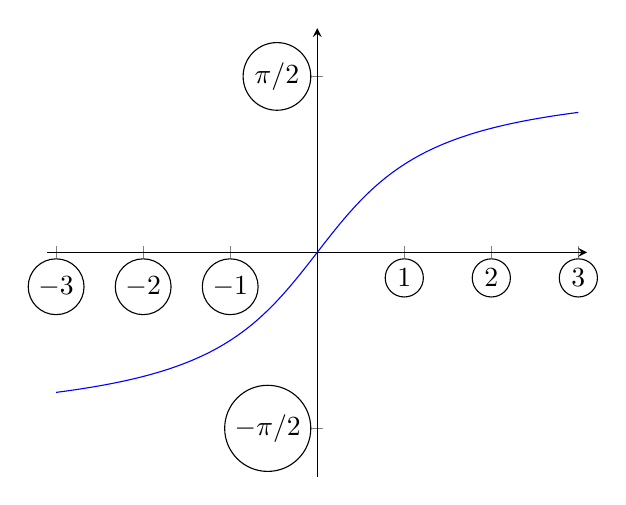
\begin{tikzpicture}
    \begin{axis}[
        domain=-3:3,
        xmin=-3.1, xmax=3.1,
        ymin=-2, ymax=2,
        samples=400,
        axis lines=middle,
        ytick={-1.57,1.57}, yticklabels={$-\pi$/2,$\pi$/2}
    ]
        \addplot+[mark=none] {atan(x)/180*pi};
    \end{axis}
\end{tikzpicture}

\item $k: x \mapsto \arc\ctg x$\quad 
$D_k=]-\infty;\infty[ \quad R_k:]0;\pi[$\\
\begin{tikzpicture}
    \begin{axis}[
        domain=-3:3,
        xmin=-3.1, xmax=3.1,
        ymin=-0.1, ymax=3.5,
        samples=400,
        axis lines=middle,
        ytick={1.57,3.14}, yticklabels={$\pi$/2,$\pi$}
    ]
        \addplot+[mark=none] {rad(90-atan(x))};
    \end{axis}
\end{tikzpicture}

\end{abc2}

\begin{enumerate}
\item Oldjuk meg valós számok halmazán
\begin{abc}
\item $\sin^6x+\cos^6x=1$;
\item $2\sin x+3\cos^2x\geq5$;
\item $(\sin x+\sqrt{3}\cos x)\cdot \sin 4x =2$.
\end{abc}
\item Határozzuk meg a következő függvények legnagyobb és legkisebb értékét:
\begin{abc}
\item $f(x)=\sin^6x+\cos^6x;\qquad x\in \mathbb{R}$
\item $h(x)=\frac{7}{2}\sqrt{(\sin x+\cos x)^2+2};\qquad x\in \mathbb{R}$

\end{abc}
\end{enumerate}

%\newpage
\subsection*{2012.03.07 -- Komplex számok}
\underline{Definíciók}: $i^2=-1,\quad \mathbb{C}=\{a+ib~|~ a,b \in \mathbb{R}\}$,

$(a+ib)+(c+id)=(a+c)+(b+d)$,

$(a+ib)(c+id)=(ac-bd)+i(ad+bc)$;

$|a+ib|=\sqrt{a^2+b^2}$;\quad $Re(a+ib)=e$,\quad $Im(a+ib)=b,$\quad$\overline{a+ib}=a-ib.$

Trigonometrikus alak: $z=a+ib$, $r=\sqrt{a^2+b^2}$, $z=r(\cos\varphi+i\sin\varphi)$

\definecolor{qqwuqq}{rgb}{0.,0.39215686274509803,0.}
\definecolor{uuuuuu}{rgb}{0.26666666666666666,0.26666666666666666,0.26666666666666666}
\begin{tikzpicture}[line cap=round,line join=round,>=triangle 45,x=1.0cm,y=1.0cm]
\draw[->,color=black] (-1,0.) -- (7,0.);
\foreach \x in {2.,4.,6.}
\draw[shift={(\x,0)},color=black] (0pt,2pt) -- (0pt,-2pt);
\draw[->,color=black] (0.,-1) -- (0.,4.1);
\foreach \y in {2.,4.}
\draw[shift={(0,\y)},color=black] (2pt,0pt) -- (-2pt,0pt);
%\clip(-3.924300151749257,-2.9589479655429174) rectangle (9.607446517450182,7.207888341866245);
\draw [shift={(0.,0.)},color=qqwuqq,fill=qqwuqq,fill opacity=0.1] (0,0) -- (0.:0.721052220383629) arc (0.:30.963756532073532:0.721052220383629) -- cycle;
\draw [->] (0.,0.) -- (5.,3.);
\draw (5.,3.)-- (5.,0.);
\draw (4.992712306994956,3.2901712777818637) node[anchor=north west] {$a+ib$};
\begin{scriptsize}
\draw [fill=uuuuuu] (0.,0.) circle (1.5pt);
\draw[color=uuuuuu] (0.9307847988338456,0.1896467301322608) node {$\varphi$};
\draw[color=black] (2.5170996836778294,1.7759616149762436) node {$r$};
\end{scriptsize}
\end{tikzpicture}


\begin{enumerate}
\item Igazoljuk a Moivre-tételt: $z_1=r_1(\cos\varphi_1+ i \sin\varphi_1),\quad z_2=r_2(\cos\varphi_2+\sin\varphi_2),$ akkor,

$z_1z_2=r_1r_2(\cos(\varphi_1+\varphi_2)+i \sin (\varphi_1+\varphi_2))$
\item Számítsuk ki:
\begin{abc}
\item $\dfrac{(i+1)^{2n}}{(i-1)^{2n-2}}$, $n>0$ egész;
\item $(1+i)^{52}$,
\item $\left(\dfrac{1+i\sqrt{3}}{1-i}\right)^{20}$.
\end{abc}
\item Legyen $\omega=-\frac{1}{2}+i\frac{\sqrt{3}}{2}$, $a,b$ tetszőleges valós számok. Számítsuk ki:
\begin{abc2}
\item $(a+b)(a+b\omega)(a+b\omega^2)$;
\item $(a\omega^2+b\omega)(b\omega^2+a\omega)$.
\end{abc2}
\end{enumerate}

%\newpage
\subsection*{2012.05.08 -- Valószínűségszámítás}
\underline{Definíciók}:

\underline{Esemény:} az elemi események halmazának részhalmaza, jelölése $A,B, ...\quad;$

$A+B$ az az esemény, amiben vagy $A$ vagy $B$ bekövetkezik;

$A\cdot B$ az az esemény, amiben $A$ is és $B$ is bekövetkezik;

$\overline{A}$ az az esemény, amiben $A$ nem következik be.

$I$ vagy $E$ a biztos esemény (mindig bekövetkezik)

$O$ a lehetetlen esemény, soha nem következik be;

\underline{$A$ valószínűsége:}
\begin{itemize}
\item $P(A)$ egy függvény, ami az eseményeken van értelmezve, 
\item $0\leq P(A) \leq 1$, 
\item ha $A\cdot B=0$, akkor $P(A+B)=P(A)+P(B)$, 
\item $A$ és $B$ függetlenek, ha $P(A\cdot B)=P(A)\cdot P(B)$. 
\end{itemize}
\underline{Binomiális elosztás:} $0\leq p \leq 1$,$\quad$ $q=1-p$,\qquad Várható értéke: $M(X)=np$

$$P(X=k)=\binom{n}{k}\cdot p^k \cdot q^{n-k}$$

\noindent
\underline{Hipergeometrikus eloszlás:} $N,M,n$  \qquad Várható értéke: $M(X)=n\frac{M}{N}$
$$P(x=k)=\frac{\binom{M}{k}\binom{N-M}{n-k}}{\binom{N}{n}}$$


\noindent
\underline{Geometrikus eloszlás:} $0\leq p\leq  1,\quad q=1-p$\qquad Várható értéke : $M(X)=\frac{1}{p}$
$$P(x=k)=q^{k-1}p$$ 

%\newpage
\subsection*{2012.03.14 -- Kombinatorika}

\underline{Definíciók}:

\begin{description}
\item[\underline{Permutációk}:] adott $n$ elemű összes lehetséges sorrendje egy-egy permutáció.

Az $n$ elem permutációinak száma: $n!$ (teljes indukció).

Ha az $n$ elem közül $k_1,k_2,...,k_r$ azonos $(k_1+k_2+...k_r=n)$ akkor az ilyen ismétléses permutációk száma: $$\frac{n!}{k_1!\cdot k_2!\cdots k_r}$$

\item[\underline{Variációk}:] adott $n$ elem közül $k$-t hányféleképpen lehet sorbarakni $(k\leq n)$ : $V_n^k=n(n-1)...(n-k+1)$.

Ismétléses variáció, ha ugyanaz az elem az elem akárhányszor szerepelhet, ezek száma: $n^k$,

\item[\underline{Kombinációk}:] $n$ elemből hányféleképpen lehet $k$-t kiválasztani (a sorrend nem számít): $$\binom{n}{k}\qquad (0\geq k\geq n).$$

Ismétléses kombinációk, ha ugyanazt az elemet többször is választhatjuk: $$\binom{n+k-1}{k-1}=\binom{n+k-1}{n}.$$

Egy $n$ elemű halmaz összes $$\binom{n}{0}+\binom{n}{1}+\binom{n}{2}+...+\binom{n}{n}=2^n.$$

\item[\underline{Logikai szita formula}:] $A,B,C$ véges halmazok $|A|$ az $A$ elemeinek száma, $$|A\cup B|=|A|+|B|-|A\cap B|;$$
$$|A\cup B\cup C|=|A|+|B|+|C|-|A\cap B|-|A\cap C|-|B\cap C|+|A\cap B\cap C|$$
Általánosítható $n$ halmazra is.

\item[\underline{A Pascal háromszög képzési szabálya}:]
$$\binom{n}{k}+\binom{n}{k+1}=\binom{n+1}{k+1}\quad\binom{n}{0}=\binom{n}{n}=1.$$

A Pascal háromszög $n$-edik sora váltakozó előjellel: $n>0,\quad n\in$ $N$
$$\binom{n}{0}-\binom{n}{1}+\binom{n}{2}-\binom{n}{3}+...+(-1)^n\binom{n}{n}=0;$$
További összegek :
$${\binom{n}{0}}^2+{\binom{n}{1}}^2+{\binom{n}{2}}^2+...+{\binom{n}{n}}^2=\binom{2n}{n};$$
$$\binom{2n}{0}-\binom{2n}{2}+\binom{2n}{4}-\binom{2n}{6}+...+(-1)^n\binom{2n}{2n}=2^n\cos n\frac{\pi}{2};$$
$$\binom{2n}{1}-\binom{2n}{3}+\binom{2n}{5}-...+(-1)^{n-1}\binom{2n}{2n-1}=2^n\sin n\frac{\pi}{2}.$$

\end{description}
\subsection*{2012.03.22 -- Számelméleti függvények}

\underline{Definíciók}:

$d$(n) az $n>0$ egész szám pozitív osztóinak száma;

$\delta (n)$ az $n>0$ egész szám pozitív osztóinak összege;

$\varphi(n)$ az $n>0$ egész, akkor az $1,2,...,n$ számok között az $n$-hez relatív prímek száma .

$n$ \underline{tökéletes szám}, ha $\delta (n)=2n$.

\noindent\underline{Tételek}:

ha $n=p_1^{\alpha_1}p_2^{\alpha_2}\ldots p_k^{\alpha_k}$ az $n>0$ prímhatványok szorzataként való előállítása, akkor
$$d(n)=(\alpha_1 +1)(\alpha_2 +1)\ldots(\alpha_k +1);$$
$$\delta(n)=\frac{p_1^{\alpha_1 +1}-1}{p_1 -1}\cdot\frac{p_2^{\alpha_2 +1}-1}{p_2 -1}\cdot\ldots\cdot\frac{p_k^
{\alpha_2 +1}-1}{p_k -1};$$
$$\varphi(n)=n\left(1-\frac{1}{p_1}\right)\left(1-\frac{1}{p_2}\right)\ldots\left(1-\frac{1}{p_k}\right);$$

$n$ akkor és csak akkor páros tökéletes szám, ha $n=2^{p-1}(2^p-1)$ alakú, ahol $p$ prím és $2^{p-1}$ is prím.

\begin{enumerate}
\item Melyik az az $n>0$ egész, szám, amely osztható $12$-vel és $14$ pozitív osztója van?
\item Igaz-e, hogy 
\begin{abc}
\item $7\mid \binom{1000}{500}$;
\item $7\mid \binom{10000}{5000}$?
\end{abc}
\item Határozzuk meg azokat a négyjegyű számokat, amelyeknek $15$ különböző pozitív osztója van. 
\end{enumerate}

%\newpage
\subsection*{2012.03.26 -- Sorozat határértéke, nevezetes sorozatok }
\underline{Definíció}: az $(a_n)$ sorozat konvergens és határértéke $A$, ha $A$ bármely környezetén kívül $a_n$-nek csak véges sok tagja van; azaz bármely $\varepsilon>0$ számhoz van olyan $n_0$ index, hogy ha $n>n_0$, akkor $|a_n-A|<\varepsilon$.

\noindent\underline{Jelölés}: $\lim\limits_{n\to\infty} a_n=A$, vagy rövidebben $a_n\to A$ ha $n\to\infty$.

\noindent\underline{Tételek}: 
Ha $a_n\to A$, $b_n\to B$, akkor $a_n\pm b_n\to A\pm B, a_n\cdot b_n\to A\cdot B$ és ha $B\not=0$, akkor $\frac{a_n}{b_n}\to\frac{A}{B}$.


Ha $(a_n)$ monoton növő $(a_n\leq a_{n+1})$ és felülről korlátos $(a_n\leq K)$, akkor $(a_n)$ konvergens.

Ha $a_n\leq c_n\geq b_n$ és $a_n\to A, b_n\to A$, akkor $c_n\to A$.

Az $\left(\left(1+\frac{1}{n}\right)^n\right)$ sorozat monoton nő és felülről korlátos, tehát konvergens, határértéke $e=2{,}71...$

Az $\left(\left(1+\frac{1}{n}\right)^{n+1}\right)$ sorozat monoton fogy, alulról korlátos, határértéke $e$.

A $(q^n)$ sorozat ha $|q|<1$ konvergens és határértéke $0$, (ha $q=1$, határértéke $1$).

Az $(1+q+...+q^{n-1})$ sorozat konvergens, ha $|q|<1$ és határértéke $\frac{1}{1-q}$.

\noindent További példák:

$\lim\limits_{n\to\infty} \left(\frac{1}{1\cdot 2}+\frac{1}{2\cdot 3}+...+\frac{1}{(n-1)\cdot n}\right)=1$;

$\lim\limits_{n\to\infty} \frac{a^n}{n!}=0$ ha $a>1$;

$\lim\limits_{n\to\infty} \frac{n^k}{a^n}=0$ ha $a>1$, $k$ adott szám.

\noindent\underline{Definíciók}:

ha $a_{n+1}-a_n=d$ állandó, akkor $(a_n)$ számtani sorozat;

ha $a_{n+1}=qa_n$, $q$ állandó, akkor $(a_n)$ mértani sorozat;

a Fibonacci sorozat:
$f_1=f_2=1,\quad f_{n+2}=f_n+f_{n+1}$.

\noindent\underline{Tételek}:

Ha $(a_n)$ számtani sorozat, akkor $a_n=a_1+(n-1)d$;

ha $(a_n)$ mértani sorozat, akkor $a_n=a_1\cdot q^{n-1}$;

Összegképletek:

számtani sorozat: $a_1+a_2+...+a_n=\frac{a_1+a_n}{2}n$;

mértani sorozat: $a_1+a_2+...+a_n=
\left\{
\begin{array}{lr} 
a_1\frac{q^n-1}{q-1} &\text{~ha~} q\ne 1\cr 
na_1 &\text{~ha~} q=1
\end{array}
\right.$. 

A Fibonacci-sorozat tulajdonságai:

$f_1+f_3+f_5+...+f_{2n-1}=f_{2n};$

$f_2+f_4+f_6+...+f_{2n}=f_{2n+1}-1;$

$f_1^2+f_2^2+...+f_n^2=f_n\cdot f_{n+1};$

$f_1\cdot f_2+f_2\cdot +...+f_{2n-1}\cdot f_{2n}=f_{2n}^2.$

%\newpage
\subsection*{2012.03.29 -- Kongruenciák, számrendszerek}
\underline{Definíció}: $a\equiv b \pmod{m},$ ha $m|a-b$.

\noindent\underline{Tételek}:

$a\equiv a\pmod{m}$ :reflexív

$a\equiv b\pmod{m} \longrightarrow b\equiv a\pmod{m}$ :szimmetrikus

$a\equiv b\pmod{m}$ és $b\equiv c\pmod{m}\longrightarrow a\equiv c\pmod{m};\qquad$ :tranzitív

$a\equiv b\pmod{m}\longrightarrow a+c=b+c\pmod{m};$

$a\equiv b$ és $c\equiv d\pmod{m} \longrightarrow a+c\equiv b+d\pmod{m};$

$a\equiv b\longrightarrow ac\equiv bd\pmod{m};$

$a\equiv b$ és $c\equiv d\pmod{m}\longrightarrow ac\equiv bd\pmod{m};$

$a\equiv b\pmod{m}\longrightarrow a^n\equiv b^n\pmod{m};$

\noindent{Kis-Fermat tétel}: ha $p$ prím, $(a,p)=1$, akkor 
$a^{p-1}\equiv 1\pmod{p}$;

\noindent{Euler tétel}: ha $(a,m)=1$, akkor 
$a^{\varphi(m)}\equiv 1\pmod{m}$;

\noindent{Wilson tétel}: ha $p$ prím, akkor 
$(p-1)!\equiv -1\pmod{p}$.

\noindent{A maradékos osztás tétele}: Tetszőleges $a$ és $b\not=0$ egész számokhoz egyértelműen léteznek olyan $q$ és $r$ pozitív egészek, hogy
$$a=qb+r\quad ;\quad 0\leq r<|b|.$$

\noindent\underline{Definíció}: Ha $a$ és $b$ adott egész számok, akkor a  $D$ egész szám az $a$ és $b$ legnagyobb közös osztója, ha $D\mid a$ és $D\mid b$, továbbá ha $d$ egészre $d\mid a$ és $d\mid b$ teljesül, akkor $d\mid D$.

Jelölése: $(a,b)=D$.

\noindent\underline{Euklédeszi algoritmus}: adott  $a,b$ egészek,

\noindent{ha} $b=0$, akkor $(a,b)=a$, ha $b\not=0$

$a=q_1b+r_1$ (ha $r_1=0$, akkor  $(a,b)=b),$

\noindent{ha}  $r_1\not=0$ $b=q_2r_1+r_2,$ ha $r_2\not=0$

$r_1=q_3r_2+r_3$, és így tovább

\ldots

\noindent{ha} az utolsó nem nulla maradék $r_n$, akkor

$r_{n-1}=q_{n+1}r_n$ és $(a,b)=r_n$.

\noindent{Az} $a>1$ alapú számrendszer: ha  tetszőleges egész szám,akkor 
$$n=b_0a^k+b_1a^{k-1}+\ldots +b_{k-1}a+b_k,$$

ahol $b_0,b_1,\ldots ,b_2$ egész számok és
$$0\leq b_i\leq a-1\qquad i=0,1,2, \ldots,k$$

az adott felírás egyértelmű.

\noindent{Igazoljuk}, hogy egy $n$ szám akkor és csak akkor osztható $a-1$-gyel, ha $b_0+b_1+\ldots+b_k$ osztható $a-1$-gyel.




	
	
\section{Csoportok}

\subsection*{2012. 04. 02.}
\begin{enumerate}
\item Készítsük el a (modulo 5) maradékosztályok összeadási és szorzási táblázatát.\\ Igazoljuk, hogy teljesülnek a következő tulajdonságok a szorzásra: kommutatív, asszociatív, az 1-gyel való szorzás nem változtat a tényezőn és minden 0-tól különböző számhoz van olyan, amivel szorozva 1-et kapunk.
\item \textbf{Definíció.} Egy $G\ne\varnothing$ halmaz és egy rajta értelmezett művelet (az ún. szorzás) \emph{csoport}, ha teljesülnek a következő ún. csoportaxiómák:
\begin{enumerate}[label=(\arabic*)]
\item $G$ bármely két elemének szorzata is $G$ eleme;
\item a szorzás asszociatív;
\item van $G$-ban egységelem $e$, hogy tetszőleges $a\in G$-re $e\cdot a=a$
\item bármely $a\in G$-hez van olyan $a^{-1}\in G$, hogy $a^{-1}\cdot a=e$ (van balinverz).
\end{enumerate}
Igazoljuk, hogy az 1. példában a mod 5 összeadás is csoport.
\item Igazoljuk, hogy minden $a\in G$-nek az $a^{-1}$, azaz a balinverz, egyben jobbinverze is.
\item Igazoljuk, hogy $e$ egyben jobbegység is.
\end{enumerate}

\subsection*{2012. 04. 04.}
\begin{enumerate}
\item Adott az $ABCD$ négyzet, jelölje $t$ az $AC$ tengelyre való tükrözést és $F$ az $O$ középpont körüli $90^\circ$-os pozitív irányú elforgatást. Írjuk fel az $ABCD$ négyzetet önmagába vivő egybevágósági transzformációkat $t$ és $f$ segítségével.
\item Igazoljuk, hogy az $f(x)=x$, $g(x)=\frac{1}{x}$, $h(x)=-x$, $j(x)=-\frac{1}{x}$ függvények csoportot alkatnak az összetettfüggvény-képzés műveletére.
\item Igazoljuk, hogy egy szabályos hatszöget önmagába vivő egybevágósági transzformációk csoportot alkotnak a kompozíció műveletére.
\item Igazoljuk, hogy a komplex ötödik egységgyökök a szorzás műveletére nézve csoportot alkotnak.
\item A szabályos háromszöget önmagába vivő egybevágósági transzformációk csoportja a $D_3$ csoport. Írjuk fel a művelettáblázatát.
\end{enumerate}

\subsection*{2012. 04. 11.}
\begin{enumerate}
\item Igazoljuk, hogy $n$ elem (pl. az 1, 2, \ldots, $n$ számok) összes permutációi a kompozíció (egymás után alkalmazás) műveletére csoportot alkotnak.\\ Ennek a csoportnak a neve: $n$-edrendű szimmetrikus csoport: $S_n$.
\item Adott a következő permutáció: $f=\left(\begin{matrix}
1&2&3&4&5&6\\
2&3&4&5&6&1\\
\end{matrix}\right)$.\\
Számítsuk ki az $f^3$, $f^5$, $f^6$ permutációkat.
\item Legyen $f=\left(\begin{matrix}
1&2&3&4&5&6&7&8\\
2&3&4&8&1&5&7&6\\
\end{matrix}\right)$ és $g=\left(\begin{matrix}
1&2&3&4&5&6&7&8\\
8&1&2&7&3&4&5&6\\
\end{matrix}\right)$.\\ Számítsuk ki a következő permutációkat: $f^2$, $g^2$, $fg$, $gf$, $f^{100}$, $g^{100}$.
\item Adottak az $f=\left(\begin{matrix}
1&2&3&4&5&6\\
2&5&1&6&4&3\\
\end{matrix}\right)$ és a $g=\left(\begin{matrix}
1&2&3&4&5&6\\
3&5&1&6&4&2\\
\end{matrix}\right)$ permutációk.\\ Oldjuk meg az $f\cdot u=g$ az $u\cdot f=g$ egyenleteket.
\item Igazoljuk, hogy a komplex $n$-edik egységgyökök a szorzás műveletére csoportot alkotnak ($n>0$ egész).
\end{enumerate}

\subsection*{2012. 04. 12.}
\begin{enumerate}
\item Oldjuk meg a következő egyenletet: $f\cdot u\cdot g=h$, ha 
\[f=\left(\begin{matrix}
1&2&3&4&5\\
5&3&1&2&4\\
\end{matrix}\right),~
g=\left(\begin{matrix}
1&2&3&4&5\\
4&2&5&1&3\\
\end{matrix}\right),~
h=\left(\begin{matrix}
1&2&3&4&5\\
5&4&3&2&1\\
\end{matrix}\right).\]
\item Egy $G$ csoportról azt mondjuk, hogy ciklikus, ha van olyan $a\in G$, hogy $a$ hatványai kiadják $G$ összes elemét. Igazoljuk, hogy
\begin{abc}
\item a komplex $n$-edik egységgyökök ($n>0$ egész) a szorzásra nézve ciklikus csoportot alkotnak;
\item egy szabályos $n$-szög középpont körüli forgatásai ciklikus csoportot alkotnak.
\end{abc}
\item Egy véges csoport rendje a csoport elemeinek száma. Egy csoportelem rendje az a legkisebb pozitív egész kitevő, amelyre emelve az elemet egységet kapunk. Igazoljuk, hogy egy elem rendje mindig osztója a csoport rendjének, ha a csoport véges.
\item Igazoljuk, hogy ha egy csoportban minden $e$-től különböző elem rendje 2, akkor a csoport kommutatív.
\item Határozzuk meg az $S_3$ csoport elemeinek rendjét.
\end{enumerate}

\subsection*{2012. 04. 18.}
\begin{enumerate}
\item A $\mathbb{C}^{*}=\mathbb{C}\setminus\{0\}$ (a komplex számok a 0 nélkül) elemei a szorzásra nézve csoportot alkotnak. Melyek ebben a csoportban azok az elemek, amelyeknek rendje 6?
\item Lehet-e egy csoportban pontosan 2 másodrendű elem?
\item Igazoljuk, hogy egy véges csoportban ha minden elem rendje 2, akkor $2^n$ számú elemből áll.
\item Legyen $G$ egy csoport, $a\in G$, $n>0$ egész. Igazoljuk, hogy a következő állítások ekvivalensek:
\begin{abc}
\item $a$ rendje $n$;
\item $\{a\}$ (az $a$ elem által generált részcsoport) $n$-edrendű.
\end{abc}
\item Igazoljuk, hogy a következő permutációk a kompozíció műveletére csoportot alkotnak:
\[e=\left(\begin{matrix}
1&2&3&4&5&6\\
1&2&3&4&5&6\\
\end{matrix}\right),~
f=\left(\begin{matrix}
1&2&3&4&5&6\\
6&4&2&5&3&1\\
\end{matrix}\right),\]
\[g=\left(\begin{matrix}
1&2&3&4&5&6\\
1&5&4&3&2&6\\
\end{matrix}\right),~
h=\left(\begin{matrix}
1&2&3&4&5&6\\
6&3&5&2&4&1\\
\end{matrix}\right).\]
\item Adjunk példát 3 elemű csoportra.
\end{enumerate}

\subsection*{2012. 04. 19.}
\begin{enumerate}
\item \textbf{Definíció.} A $G_1$ és $G_2$ csoport \emph{izomorf}, ha van olyan $f$ függvény, hogy minden $a\in G_1$-re $f(a)\in G_2$, $f$ kölcsönösen egyértelmű és ha $a,b\in G_1$, akkor $f(a\cdot b)=f(a)\cdot f(b)$.\\
Igazoljuk, hogy csak két nem izomorf 4 elemű csoport van.
\item Igazoljuk, hogy minden végtelen ciklikus csoport izomorf az egész számoknak az összeadás műveletére alkotott csoportjával.
\item Igazoljuk, hogy egy $n$-edrendű ciklikus csoport izomorf az $n$-edik egységgyököknek a szorzás műveletére alkotott csoportjával.
\item Határozzuk meg az $S_3$ csoport összes részcsoportját.
\item Adott az $ABCD$ rombusz (nem négyzet). Adjuk meg a rombuszt önmagába vivő egybevágósági transzformációkat és igazoljuk, hogy ezek a kompozícióra (egymás után végzésre) csoportot alkotnak. Írjuk fel a művelettáblázatot.
\end{enumerate}

\section{Lineáris algebra}

\subsection*{2012.04.23.}
\begin{enumerate}
\item Oldjuk meg a következő lineáris egyenletrendszert:
\begin{align*}
a_{11}x_1+a_{12}x_2&=b_1,\cr
a_{21}x_1+a_{22}x_2&=b_2,
\end{align*}
ahol $a_{11},a_{12},a_{21},a_{22}$ adott számok és
$a_{11}a_{22}-a_{21}a_{12}\ne 0$.

\medskip
\noindent
\underline{Definíció:} Az $\deta{a_{11}}{a_{12}}{a_{21}}{a_{22}}$ szimbólumot $2\times 2$-es determinánsnak nevezzük és értéke $a_{11}a_{22}-a_{21}a_{12}$.\\ Az
$\detb{a_{11}}{a_{12}}{a_{13}}{a_{21}}{a_{22}}{a_{23}}{a_{31}}{a_{32}}{a_{33}}$ egy $3\times 3$-as determináns, értéke:
$$
a_{11}a_{22}+a_{33}+
a_{12}a_{23}+a_{31}+
a_{13}a_{21}+a_{32}-
a_{13}a_{22}+a_{31}-
a_{12}a_{21}+a_{33}-
a_{11}a_{23}+a_{32}.
$$
\item Számítsuk ki a következő determinánsok értékét:
\begin{abc4}
\item $\detb{1}{-3}{2}{4}{3}{-5}{2}{1}{0}$;
\item $\deta{\cos x}{-\sin x}{\sin x}{\cos x}$;
\item $\detb{0}{1}{0}{0}{0}{1}{1}{0}{0}$;
\item $\detb{\sin 2x}{-\cos 2x}{1}{\sin x}{-\cos x}{\cos x}{\cos x}{\sin x}{\sin x}$.
\end{abc4}

\item Oldjuk meg:
\begin{abc2}
\item $\detb{2}{-1}{3}{1}{x}{-1}{-5}{2}{7}=0$;
\item $\detb{x^2}{4}{8}{x}{2}{3}{1}{1}{1}=0$.
\end{abc2}
\end{enumerate}

\subsection*{2012.04.25.}
\begin{enumerate}
\item Igazoljuk, hogy ha egy determináns egy sorában vagy egy oszlopában minden elem 0, akkor a determináns értéke 0.
\item Ha egy determináns egy sorának vagy egy oszlopának minden elemét egy $\lambda$ számmal szorozzuk, akkor a determináns értéke is $\lambda$-val szorzódik.
\item Ha egy determináns egy sorának vagy egy oszlopának minden eleme egy kéttagú összeg, akkor a determináns két determináns összege, egyikben az illető sort az összegek egyik tagjai adják, a másikban a megfelelő sort a másik tagok adják.
\item Ha a determináns főátlója felett mindenütt 0 áll, akkor a determináns értéke a főátlóban álló elemek szorzata.
\item Ha egy determináns két sorát felcseréljük, akkor értéke $-1$-gyel szorzódik.
\item Számoljuk ki a következő determinánsokat:
\begin{abc3}
\item $\detb{1}{2}{2}{2}{2}{2}{2}{2}{3}$
\item $\detb{x}{y}{x+y}{y}{x+y}{x}{x+y}{x}{y}$
\item $\begin{vmatrix}
1&a&a&a\\
0&2&a&a\\
0&0&3&a\\
0&0&0&4
\end{vmatrix}
$;
\item $
\begin{vmatrix}
1&0&0&0\\
2&3&4&5\\
3&4&5&2\\
4&5&2&3
\end{vmatrix}
$;
\item $
\begin{vmatrix}
0&1&0&0\\
2&3&4&5\\
3&4&5&2\\
4&5&2&3
\end{vmatrix}
$.
\end{abc3}
\end{enumerate}

\subsection*{2012.04.26.}
\begin{enumerate}
\item Ha egy determináns két sora azonos, akkor a determináns értéke 0.
\item Ha egy determináns egyik sorához hozzáadjuk egy másik sor $\lambda$-szorosát, akkor a determináns értéke nem változik.
\item A determináns értéke nem változik, ha sorait és oszlopait felcseréljük.
\item Ha egy determinánsban az első sor első eleme nem 0, akkor értéke az első sor első eleme szorozva azzal a determinánssal, amit úgy kapunk, hogy az első sort és az első oszlopot elhagyjuk. A tétel általánosítható.
\item Számítsuk ki a következő determinánsokat:
\begin{abc4}
\item $\detb{1}{0}{0}{2}{2}{1}{3}{3}{2}$;
\item $\begin{vmatrix}
1&0&0&2 \\
3&0&0&4 \\
0&5&6&0 \\
0&7&8&0
\end{vmatrix}$;
\item  $\begin{vmatrix}
1&2&3&4 \\
2&1&2&3 \\
3&2&1&2 \\
4&3&2&1
\end{vmatrix}$;
\item  $\begin{vmatrix}
3&1&5&8 \\
4&-2&-1&7 \\
6&3&2&1 \\
7&4&4&5
\end{vmatrix}$.
\end{abc4}
\item Oldjuk meg a következő egyenleteket:
\begin{abc2}
\item $\begin{vmatrix}
1&1&4&4 \\
-1&3-x^2&3&3 \\
7&7&5&5 \\
-7&-7&6&x^2-3
\end{vmatrix}=0$;
\item $\begin{vmatrix}
1&2&3&4 \\
-2&2-x&1&7 \\
3&6&4+x&12 \\
-4&x-14&2&3
\end{vmatrix}=0$;
\end{abc2}
\end{enumerate}


\subsection*{2012.05.02.}
\begin{enumerate}
\item \underline{Definíció:} az $e$-edrendű determináns $a_{ik}$ eleméhez tartozó előjelezett aldetermináns az az ($n-1$)-edrendű determináns a $(-1)^{i+k}$ előjellel ellátva, amely az eredetiből úgy következik, hogy az $i$-edik sort és a $k$-adik oszlopot elhagyjuk. Jele: $A_{ik}$. Igazoljuk, hogy a determináns értékét megkapjuk, ha egy sorának elemeit megszorozzuk a hozzájuk tartozó előjelezett aldeterminánsokkal és a szorzatokat összeadjuk (kifejtési tétel):$$D=a_{i1}A_{i1}+a_{i2}A_{i2}+\ldots+a_{in}A_{in}.$$
\item Számítsuk ki a következő determinánsok értékét:
\begin{abc3}
\item $\begin{vmatrix}
1&2&3&4\\
2&3&4&1\\
3&4&1&2\\
4&1&2&3
\end{vmatrix}$;
\item $\begin{vmatrix}
5&6&0&0&0\\
1&5&6&0&0\\
0&1&5&6&0\\
0&0&1&5&6\\
0&0&0&1&5
\end{vmatrix}$;
\item $\begin{vmatrix}
1&2&2&\ldots&2\\
2&2&2&\ldots&2\\
2&2&3&\ldots&2\\
\vdots&&&&\vdots\\
2&2&2&\ldots&n
\end{vmatrix}$;
\item $\begin{vmatrix}
1&1&0&0\\[0.4em]
1&\binom21&\binom22&0\\[0.4em]
1&\binom31&\binom32&\binom33\\[0.4em]
1&\binom41&\binom42&\binom43
\end{vmatrix}$;
\item $\begin{vmatrix}
1&1&0&0&\ldots&0\\[0.4em]
1&\binom21&\binom22&0&\ldots&0\\[0.4em]
1&\binom31&\binom32&\binom33&\ldots&0\\[0.4em]
\vdots&&&\ddots&&\vdots\\[0.4em]
1&\binom n1&\binom n2&\binom n3&\ldots&\binom{n}{n-1}
\end{vmatrix}$;
\item $\begin{vmatrix}
1&a&a&\ldots&a&a\\
a&2&a&\ldots&a&a\\
a&a&3&\ldots&a&a\\
\vdots&&&&&\vdots\\
a&a&a&\ldots&n&a\\
a&a&a&\ldots&a&a
\end{vmatrix}$.
\end{abc3}
\end{enumerate}


\subsection*{2012.05.03.}
\begin{enumerate}
\item Igazoljuk az u.n. Cramer-szabályt: ha az
\begin{align*}
a_{11}x_1+a_{12}x_2+\ldots+a_{1n}x_n&=b_1\\
a_{21}x_1+a_{22}x_2+\ldots+a_{2n}x_n&=b_2\\
\ldots\\
a_{n1}x_1+a_{n2}x_2+\ldots+a_{nn}x_n&=b_n
\end{align*}
egyenletrendszer determinánsa $\ne 0$, azaz
$$D=\begin{vmatrix}
a_{11}&a_{12}&\ldots&a_{1n}\\
a_{21}&a_{22}&\ldots&a_{2n}\\
&\ldots&&\\
a_{n1}&a_{n2}&\ldots&a_{nn}\\
\end{vmatrix}\ne 0,$$
akkor
$$
x_1=\frac{D_1}{D},\quad
x_2=\frac{D_2}{D},\quad
\ldots,\quad
x_n=\frac{D_n}{D},
$$
ahol $D_i$ úgy keletkezik $D$-ből, hogy az $i$-dik oszlopát az egyenletrendszer jobb oldalán álló számokra cseréljük ki.
\item Oldjuk meg a következő egyenletrendszereket:
\begin{abc3}
\item \begin{align*}
x_1-3x_2-4x_3&=4,\\
2x_1+x_2-3x_3&=-1,\\
3x_1-2x_2+x_3&=11.
\end{align*}
\item
\begin{align*}
x+y+z&=1,\\
ax+by+cz&=d,\\
a^2x+b^2y+c^2z&=d^2.
\end{align*}
\item
\begin{align*}
x_1+2x_2-x_3+3x_4&=0,\\
3x_1-x_2+x_3-5x_4&=-12,\\
2x_1+2x_2+x_3-4x_4&=-13,\\
x_1-3x_2-6x_3+x_4&=1.
\end{align*}

\end{abc3}
\end{enumerate}


\subsection*{2012.05.10.}
\begin{enumerate}
\item Oldjuk meg a Cramer-szabály felhasználásával:
\begin{abc2}
\item \begin{align*}
\lambda x+y+z&=1,\\
x+\lambda y + z &= \lambda,\\
x+y+\lambda z&= \lambda^2;\\
(\lambda\ne 1, \lambda&\ne -2.)
\end{align*}
\item \begin{align*}
a^2x+ay+z&=a^3,\\
b^2x+by+z&=b^3,\\
c^2x+cy+z&=c^3.\\
(a\ne b, a\ne c&, b\ne c)
\end{align*}
\item \begin{align*}
(1+i)x-2iy&=-2,\\
(1-i)x+(2-i)y&=3-3i.
\end{align*}
\item \begin{align*}
2x-(9a^2-2)y&=3a,\\
x+y&=1.\\
(a&\ne 0)
\end{align*}
\end{abc2}
\end{enumerate}


\subsection*{2012.05.14.}
\underline{Definíció:} Egy $n$ sorból és $k$ oszlopból álló téglalap alakú számtáblázatot \underline{mátrixnak} nevezünk. \underline{Négyzetes mátrixot} kapunk, ha $n=k$.
\begin{enumerate}
\item Oldjuk meg a következő egyenletrendszert a mátrix jelölés felhasználásával:
\begin{align*}
x_1+3x_2+3x_3&=0,\\
2x_1-x_2+3x_3&=0,\\
3x_1-5x_2+4x_3&=0,\\
x_1+17x_2+4x_3&=0.
\end{align*}
\item A következő egyenletrendszert is oldjuk meg:
\begin{align*}
x_1+x_2+5x_3&=-7,\\
2x_1+x_2+x_3&=2,\\
x_1+3x_2+x_3&=5,\\
2x_1+3x_2-3x_3&=14.
\end{align*}

\item Oldjuk meg:
 $$\begin{pmatrix}[cccc|c]
 1&2&3&4&11\\
 2&3&4&1&12\\
 3&4&1&2&13\\
 4&1&2&3&14
 \end{pmatrix}$$
\end{enumerate}


\subsection*{2012.05.16.}
\underline{Definíciók:} Azonos típusú mátrixokat össze lehet adni, az összeadást komponensenként végezzük. Egy $n\times k$-as és egy $k\times l$-es mátrixot sor-oszlop szorzással lehet összeszorozni, az eredmény egy $n\times l$-es mátrix lesz. Például:
$$
\begin{pmatrix}
1&2&3\\
2&1&1
\end{pmatrix}\cdot
\begin{pmatrix}
2&0\\
1&2\\
1&1
\end{pmatrix}=
\begin{pmatrix}
1\cdot 2+2\cdot 1+3\cdot 1& 1\cdot 0+2\cdot 2+3\cdot 1\\
2\cdot 2+1\cdot 1+1\cdot 1& 2\cdot 0+1\cdot 2+1\cdot 1
\end{pmatrix}=
\begin{pmatrix}
7&7\\
6&3
\end{pmatrix}
$$
\begin{enumerate}
\item Végezzük el a következő szorzásokat:
\begin{abc2}
\item $\matb{2}{1}{1}{5}{2}{3}{6}{5}{2}
\matb{1}{3}{2}{-3}{-4}{-5}{2}{1}{3}$;
\item $
\matb{3}{4}{9}{2}{-1}{6}{5}{3}{5}
\matb{5}{6}{4}{8}{9}{7}{-4}{-5}{-3}
$;
\item $
\begin{pmatrix}
1&-3&3&-1\\
1&3&-5&1
\end{pmatrix}
\begin{pmatrix}
1&1\\
1&2\\
1&1\\
1&-2
\end{pmatrix}
$;
\item $
\mata{5}{-4}{6}{-5}^n
$, $n>0$ egész;
\item $
\matb{2}{1}{0}{0}{1}{0}{0}{0}{2}^n
$, $n>0$ egész;
\item $
\mata{\cos \varphi}{-\sin \varphi}{\sin \varphi}{\cos \varphi}^n
$, $n>0$ egész.
\end{abc2}
\end{enumerate}


\subsection*{2012.05.17.}
\begin{enumerate}
\item Végezzük el a következő műveleteket:
\begin{abc2}
\item $
\begin{pmatrix}
1&1&1\\
4&1&0
\end{pmatrix}\cdot
\begin{pmatrix}
-1&2\\
4&5\\
6&-1
\end{pmatrix}
$;
\item $
\matb{2}{-1}{3}{1}{3}{-1}{4}{5}{1}\cdot
\begin{pmatrix}
-8\\
5\\
7
\end{pmatrix}
$.
\end{abc2}

\item Számítsuk ki a következő mátrixok inverzét:
\begin{abc2}
\item $\matb{2}{-3}{-4}{-1}{7}{2}{3}{1}{-6}$;
\item $\matb{1}{2}{3}{1}{3}{4}{1}{4}{3}$.
\end{abc2}
\item Legyen $A=\mata{3}{2}{4}{3}$ és $B=\mata{-1}{7}{3}{5}$. Oldjuk meg a következő egyenleteket: $A\cdot X = B, \qquad Y\cdot A=B$.

\item Igazoljuk, hogy az $\matb{1}{2}{-2}{1}{0}{3}{1}{3}{0}$ mátrix gyöke az 
$f(x)=x^3-x^2-9x+9$ polinomnak.
\end{enumerate}


\subsection*{2012.05.21.}
\begin{enumerate}
\item Igazoljuk, hogy a következő mátrixok csoportot alkotnak a szorzás műveletére:
\begin{abc2}
\item $\left\{\mata{a}{-b}{b}{a}~|~a,b\in\mathbb{R},\quad a^2+b^2>0\right\}$;
\item $\left\{\mata{a}{3b}{b}{a}~|~a,b\in\mathbb{R},\quad a^2+b^2>0\right\}$.
\end{abc2}
\item \underline{Definíció:} egy mátrix rangja $r$, ha a mátrix elemeiből készíthető minden $r+1$-edrendű aldetermináns 0, de van olyan $r$-edrendű aldetermináns, ami nem 0. Számítsuk ki a következő mátrix rangját:
$$\begin{pmatrix}
6&9&7&9\\
4&6&-2&5\\
4&6&18&8
\end{pmatrix}$$
\item Igazoljuk, hogy a mátrix rangja nem változik, ha

(1) csupa 0-ból álló sorát vagy oszlopát elhagyjuk;

(2) valamelyik sorát vagy oszlopát egy $\lambda\ne 0$ számmal szorozzuk;

(3) egyik sorának (vagy oszlopának) többszörösét egy másik sorához (ill. oszlopához) adjuk.
\item Számítsuk ki a következő mátrix rangját:
$$
\begin{pmatrix}
4&9&0&7&2\\
-1&1&6&0&3\\
0&-1&2&1&-2\\
4&-3&-1&9&6
\end{pmatrix}
$$
\end{enumerate}


\subsection*{2012.05.23.}
\begin{enumerate}
\item Igazolható, hogy egy lineáris egyenletrendszernek akkor és csak akkor van megoldása, ha az egyenletrendszer mátrixának és a kibővített mátrixának rangja megegyezik.
\item Döntsük el, hogy a következő egyenletrendszereknek van-e megoldása:
\begin{abc2}
\item \begin{align*}
x_1-3x_2+4x_3+2x_4&=1,\\
2x_1+4x_2-3x_3+3x_4&=-1,\\
3x_1+x_2+2x_3-x_4&=0,\\
12x_1+4x_2+7x_3+2x_4&=0.
\end{align*}
\item \begin{align*}
x_1+x_2+x_3-3x_4&=1,\\
x_1+x_2-3x_3+x_4&=-1,\\
x_1-3x_2+x_3+x_4&=0,\\
-3x_1+x_2+x_3+x_4&=0.
\end{align*}
\end{abc2}
\item Számítsuk ki a következő mátrix rangját:
$$
\begin{pmatrix}
-1&-3&-2&1&-1\\
4&1&2&4&1\\
-6&9&-10&-2&6\\
4&6&1&12&-3
\end{pmatrix}
$$
\item Határozzuk meg a következő mátrix inverzét:
$$
\begin{pmatrix}
1&1&1&1\\
1&1&-1&-1\\
1&-1&1&-1\\
1&-1&-1&1
\end{pmatrix}
$$
\end{enumerate}


\subsection*{2012.05.31. -- Determinánsok, mátrixok}
\begin{enumerate}
\item Számítsuk ki a következő determinánsok értékét:
\begin{abc2}
\item $
\begin{vmatrix}
1&3&3&1\\
1&1&3&3\\
3&1&1&3\\
3&3&1&1
\end{vmatrix}
$;
\item $
\begin{vmatrix}
1&2&3&\ldots&n\\
1&a&3&\ldots&n\\
1&2&a&\ldots&n\\
&&\vdots&\ddots&\\
1&2&3&\ldots&a
\end{vmatrix}
$
\end{abc2}

\item Számítsuk ki a következő mátrix inverzét:

$$
\begin{pmatrix}
1&1&0&0\\
-1&0&1&1\\
0&0&1&1\\
1&1&1&0
\end{pmatrix}
$$

\item Oldjuk meg a Cramer-szabály felhasználásával:

\begin{align*}
x_1-x_2+2x_3&=11,\\
x_1+2x_2-x_3&=11,\\
4x_1-3x_2-3x_3&=24.
\end{align*}

\item Oldjuk meg a következő egyenletrendszert:

\begin{align*}
-2x_1-x_2-3x_3+4x_4&=5,\\
2x_1+x_2+2x_3-3x_4&=-3,\\
4x_1+2x_2+x_3-3x_4&=0,\\
2x_1+x_2-x_4&=1,\\
2x_1+x_2-x_3&=3.
\end{align*}
\end{enumerate}














